\chapter{Discrétisation, algorithmes et exemples}
\label{chap:alorithme}
\minitoc

\[\]

Dans ce chapitre, nous adoptons une approche discrète en adaptant sur des maillages triangulaires les différents algorithmes exposés dans le chapitre \ref{chap:theoritical}. Pour ce faire, nous commençons par mettre en place le cadre discret dans lequel nous travaillons en présentant une représentation discrète des champs de croix sur des maillages triangulaires. Par la suite, nous revenons sur les notions de points singuliers, d'indices, et de lignes de champs par rapport à cette représentation, puis nous étudions le lien entre le champ continu et le champ discret.

Nous présentons ensuite l'adaptation de l'algorithme de partitionnement par rapport au cadre discret évoqué précédemment, puis quelques méthodes de paramétrisation des partitions issues de l'algorithme de partitionnement. Par la suite, nous abordons l'opération d'alignement mise en place dans le cadre discret, et nous montrons dans quel sens le partitionnement obtenu sur le maillage triangulaire est bien un partitionnement ayant des partitions de quatre côtés, permettant ainsi d'aboutir à un maillage quadrilatéral.

\section{Représentation discrète}
\label{sec:repr_discrete}

Soit $\Omega$, un domaine compact et connexe de $\mathbb{R}^2$ avec une frontière $\partial\Omega$ qui est lisse par morceaux et soit $\bar{u}$ un champ de croix presque-$\mathcal{C}^1$ sur $\Omega$.

\subsection{Maillage triangulaire}
\label{subsec:mesh_tri}

Considérons maintenant un maillage triangulaire $\Omega_h$ de $\Omega$. Par là, nous entendons que $\Omega_h$ est une surface polygonale compacte de $\mathbb{R}^2$ représentant une triangulation conforme (au sens des éléments finis) de $\Omega$. Autrement dit, $\Omega_h$ est formé par l'union de $N_t$ triangles fermés non vide ($\Omega_h=\cup_{k=1}^{N_t}T_k$) tel que tout intersection entre deux triangles est soit vide, soit un sommet, soit une arête. De plus, tous les sommets de $\Omega_h$ appartiennent à $\Omega$. Nous noterons $\mathcal{T}_h$ l'ensemble des triangles formant $\Omega_h$, l'indice $h$ faisant référence à la finesse du maillage, que l’on définit par le diamètre maximal des triangles constituant $\Omega_h$,
$$
h:=\max_{T\in\mathcal{T}_h} diam(T).
$$
Le diamètre d’un triangle est la distance maximale entre deux points du triangle. La condition $h\rightarrow 0$ signifie que tous les triangles $T_k$ ont un diamètre qui tend vers $0$. Ainsi on a $\bar{\Omega}=\Omega_h$ lorsque $h$ tend vers $0$. Nous notons $A_h$ et $S_h$ les ensembles respectivement des sommets et des arêtes de $\Omega_h$. Pour tout $p\in\Omega_h$, nous désignons par $T_p$ la partie du plan formé par l'ensemble des triangles de $\Omega_h$ contenant $p$:
$$T_p=\displaystyle\cup_{T\in\mathcal{T}_h\atop~p\in T~}T.$$

\subsection{Champ de croix}
\label{subsec:discr_champ_de_croix}

Etant donné les valeurs nodales $\bar{u}(s)$ de $\bar{u}$ donné sur les sommets $s$ de $\Omega_h$, nous cherchons à construire une représentation du champ de croix $\bar{u}$ sur le maillage triangulaire $\Omega_h$. Pour ce faire, nous allons nous orienter en nous basant sur les différentes opérations que nous devrons effectuer sur cette représentation en prenant comme modèle les opérations réalisées sur $\bar{u}$ dans le chapitre \ref{chap:theoritical}. Observons que nous devrons calculer la variation de l'angle des croix le long d'un arc paramétré, notamment pour déterminer l'indice de points ou pour quantifier la variation du champ de croix dans une partie du domaine. En limitant ces arcs aux bords des triangles, il devient évident qu'il est possible de simplifier le problème en connaissant la variation des croix le long des arêtes du triangle. En d'autres termes, il nous faut une notion de variation d'angle entre deux croix quelconques. Nous avons alors la définition suivante:

\begin{definition}
Soient deux croix $\mathbf{c}_1,\mathbf{c}_2$ non nulles. L'angle signé entre $\mathbf{c}_1$ et $\mathbf{c}_2$ noté $\delta\theta(\mathbf{c}_1,\mathbf{c}_2$) est l'unique élément de l'ensemble:
$$
\{\delta\theta(\mathbf{c}_1,\mathbf{c}_2)\}:=\left\{\theta_{\mathbf{c}_2}-\theta_{\mathbf{c}_1}+k\frac{\pi}{2},~k\in\mathbb{Z}\right\}\cap\left]-\frac{\pi}{4}, \frac{\pi}{4}\right[.
$$
\end{definition}
Cette fonction mesure la variation angulaire entre $\mathbf{c}_1$ et $\mathbf{c}_2$ de $\mathbf{c}_1$ vers $\mathbf{c}_2$. Autrement dit, on a:
$$
\theta_{\mathbf{c}_2}=\theta_{\mathbf{c}_1}+\delta\theta(\mathbf{c}_1,\mathbf{c}_2).
$$
Une conséquence directe de cette définition est l'antisymétrie de l'angle, ce qui se traduit par:
$$
\delta\theta(\mathbf{c}_1, \mathbf{c}_2)=-\delta\theta(\mathbf{c}_2,\mathbf{c}_1).
$$
Nous dirons que $\delta\theta(\mathbf{c}_1,\mathbf{c}_2$) n'est pas défini lorsque $|\theta_{\mathbf{c}_2}-\theta_{\mathbf{c}_1}|=\pi/4$.

\begin{definition}
\label{def:triangle_singulier}
 Soit triangle $T$ de sommets $s_1$, $s_2$ et $s_3$. $T$ est dit singulier s'il vérifie l'une des propriétés suivantes:\\
 \begin{itemize}
  \item[1.] il existe $i\in\llbracket 1, 3\rrbracket$ tel que $\bar{u}(s_i)=0$,\\%[-0.2cm]
  \item[2.] il existe  $i,j\in\llbracket 1, 3\rrbracket$, tel que  $\delta\theta(\bar{u}(s_i),\bar{u}(s_j))$ n'est pas défini,\\%[-0.2cm]
  \item[3.] pour tout $i\in\llbracket 1, 3\rrbracket$, $\bar{u}(s_i)\neq 0$ et $\sum_{i=1}^3\delta\theta(\bar{u}(s_i),\bar{u}(s_{i+1}))\neq 0$ où on a posé $\bar{u}(s_4):=\bar{u}(s_3)$.\\[-0.2cm]
 \end{itemize}
\end{definition}

L'ensemble constitué des triangles singuliers peut être subdivisé en plusieurs parties, dont les parties du plan correspondantes seront appelées \emph{zones singulières}. Pour assembler ces partitions, on regroupe les triangles singuliers entre eux avec la contrainte que deux triangles singuliers adjacents font partie de la même zone singulière. Sur la figure \ref{fig:zone_singuliere}, nous présentons un exemple illustrant la construction de zones singulières. On se donne une configuration où la couleur rouge indique les emplacements où l'une des propriétés de la définition \ref{def:triangle_singulier} est vérifiée. Nous affichons ensuite les zones singulières correspondantes en bleu. Cette configuration particulière conduit à la création de cinq zones singulières que nous présentons sur la même figure. Dans la suite, nous utiliserons la notation $\mathbf{Z}=\cup_{i=1}^{N_Z}Z_i$ pour représenter la partie du plan occupé par l'ensemble des zones singulières. Ici, $Z_i$ désigne une zone singulière spécifique, et $N_z$ représente le nombre total de zones singulières. Ce nombre est nécessaire fini puisque le champ de croix $\bar{u}$ possède un nombre fini de points singuliers. Nous associons ensuite à chaque zone singulière $Z\in \mathbf{Z}$ un point arbitrairement choisi dans $Z$, noté $S_Z$ tel que $Z$ soit étoilé par rapport à $S_Z$ (par exemple, lorsque $Z$ est réduit à un unique triangle, on peut choisir $S_Z$ comme le barycentre du triangle en question).

\begin{figure}[htpb]
\centering
\begin{subfigure}{0.49\textwidth}
    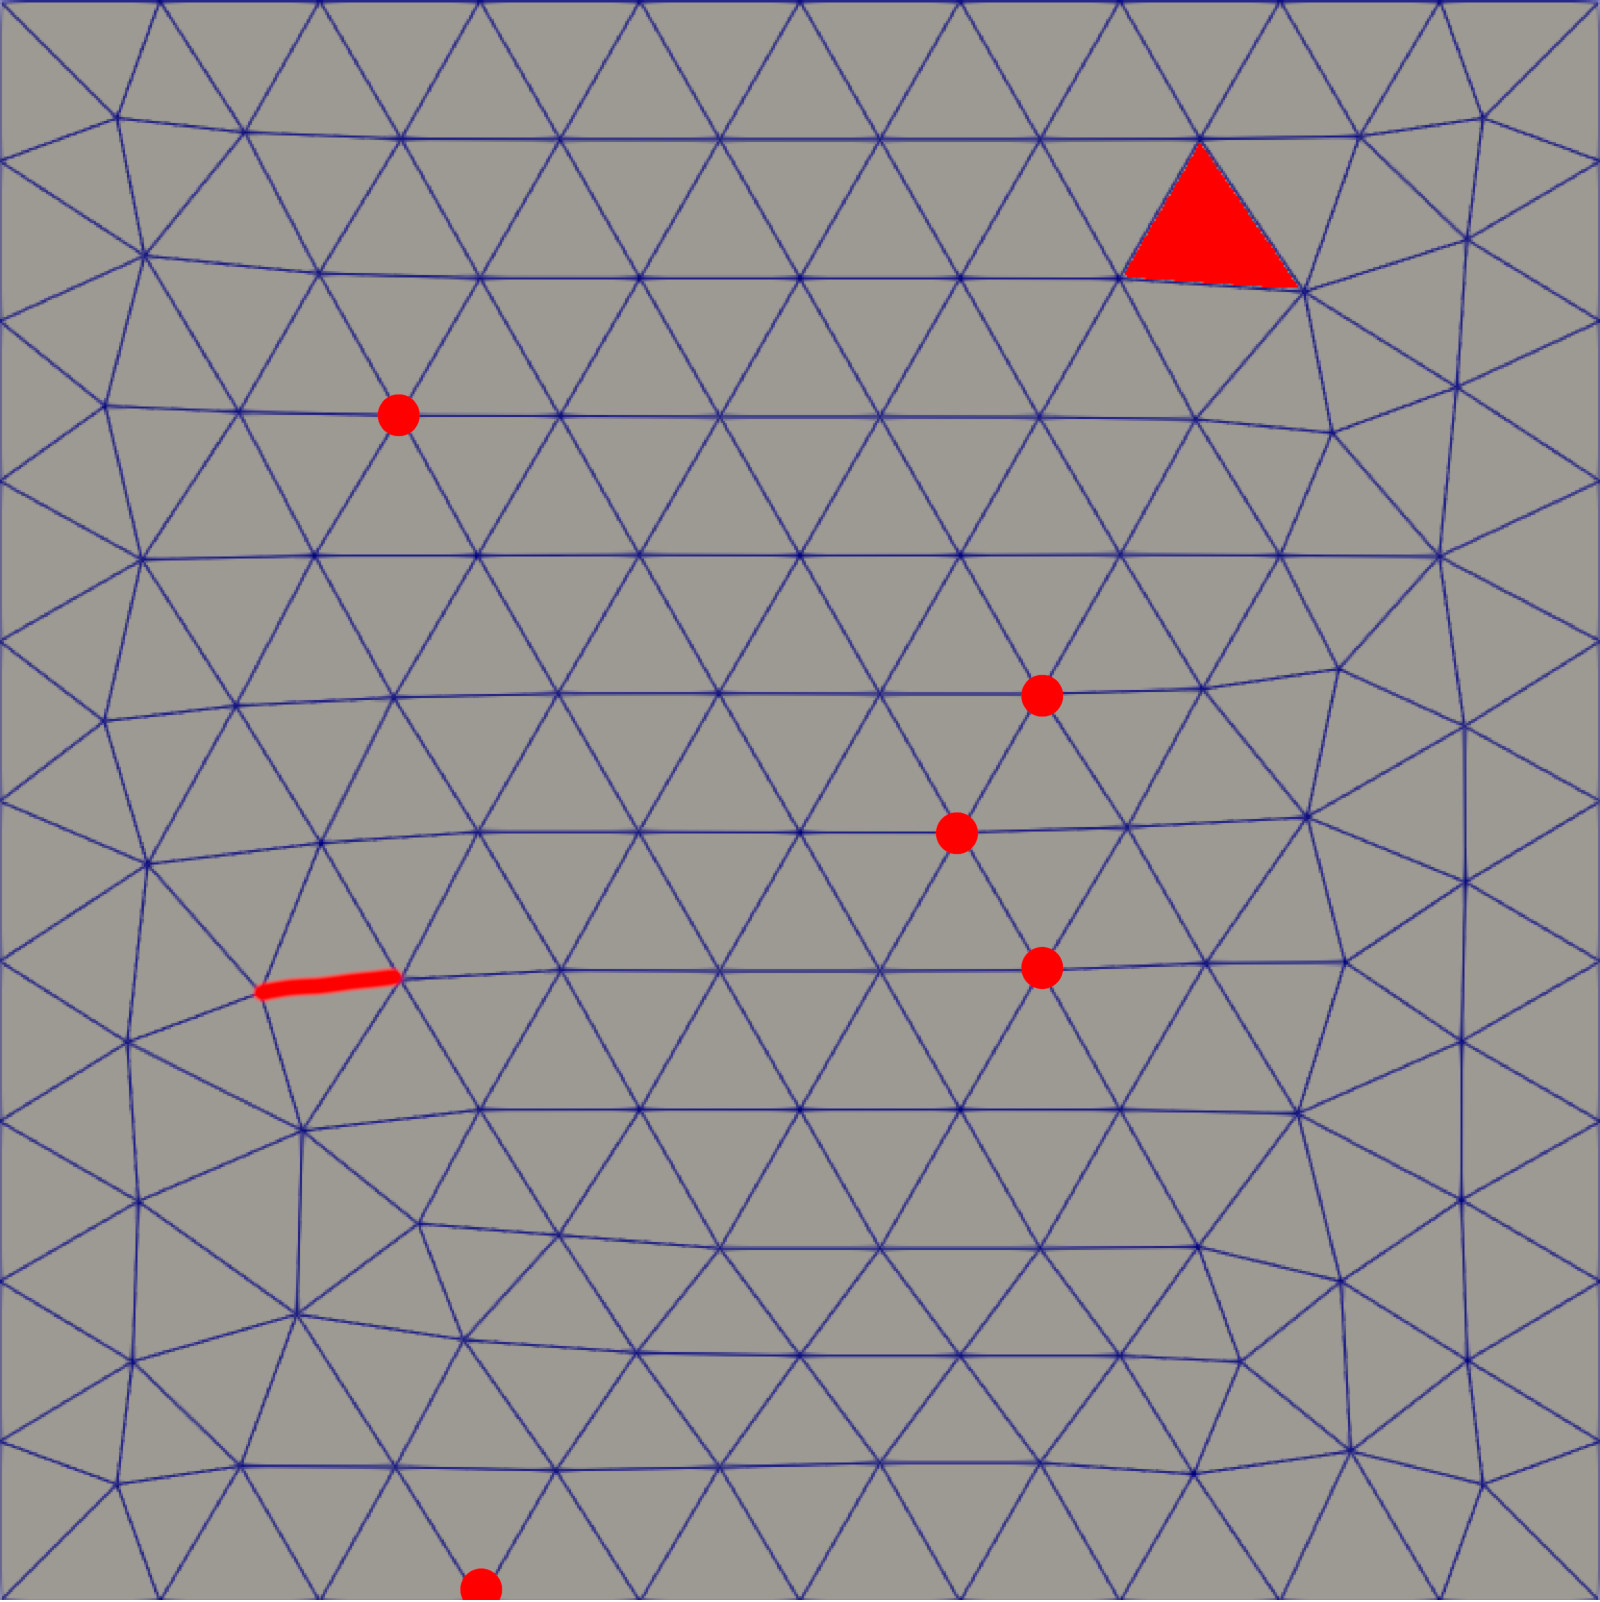
\includegraphics[width=\textwidth]{images/zone_singuliere_1.pdf}
    %\caption{Insertion de $D$.}
    %\label{fig:quad_eclatement}
\end{subfigure}
\hfill
\begin{subfigure}{0.49\textwidth}
    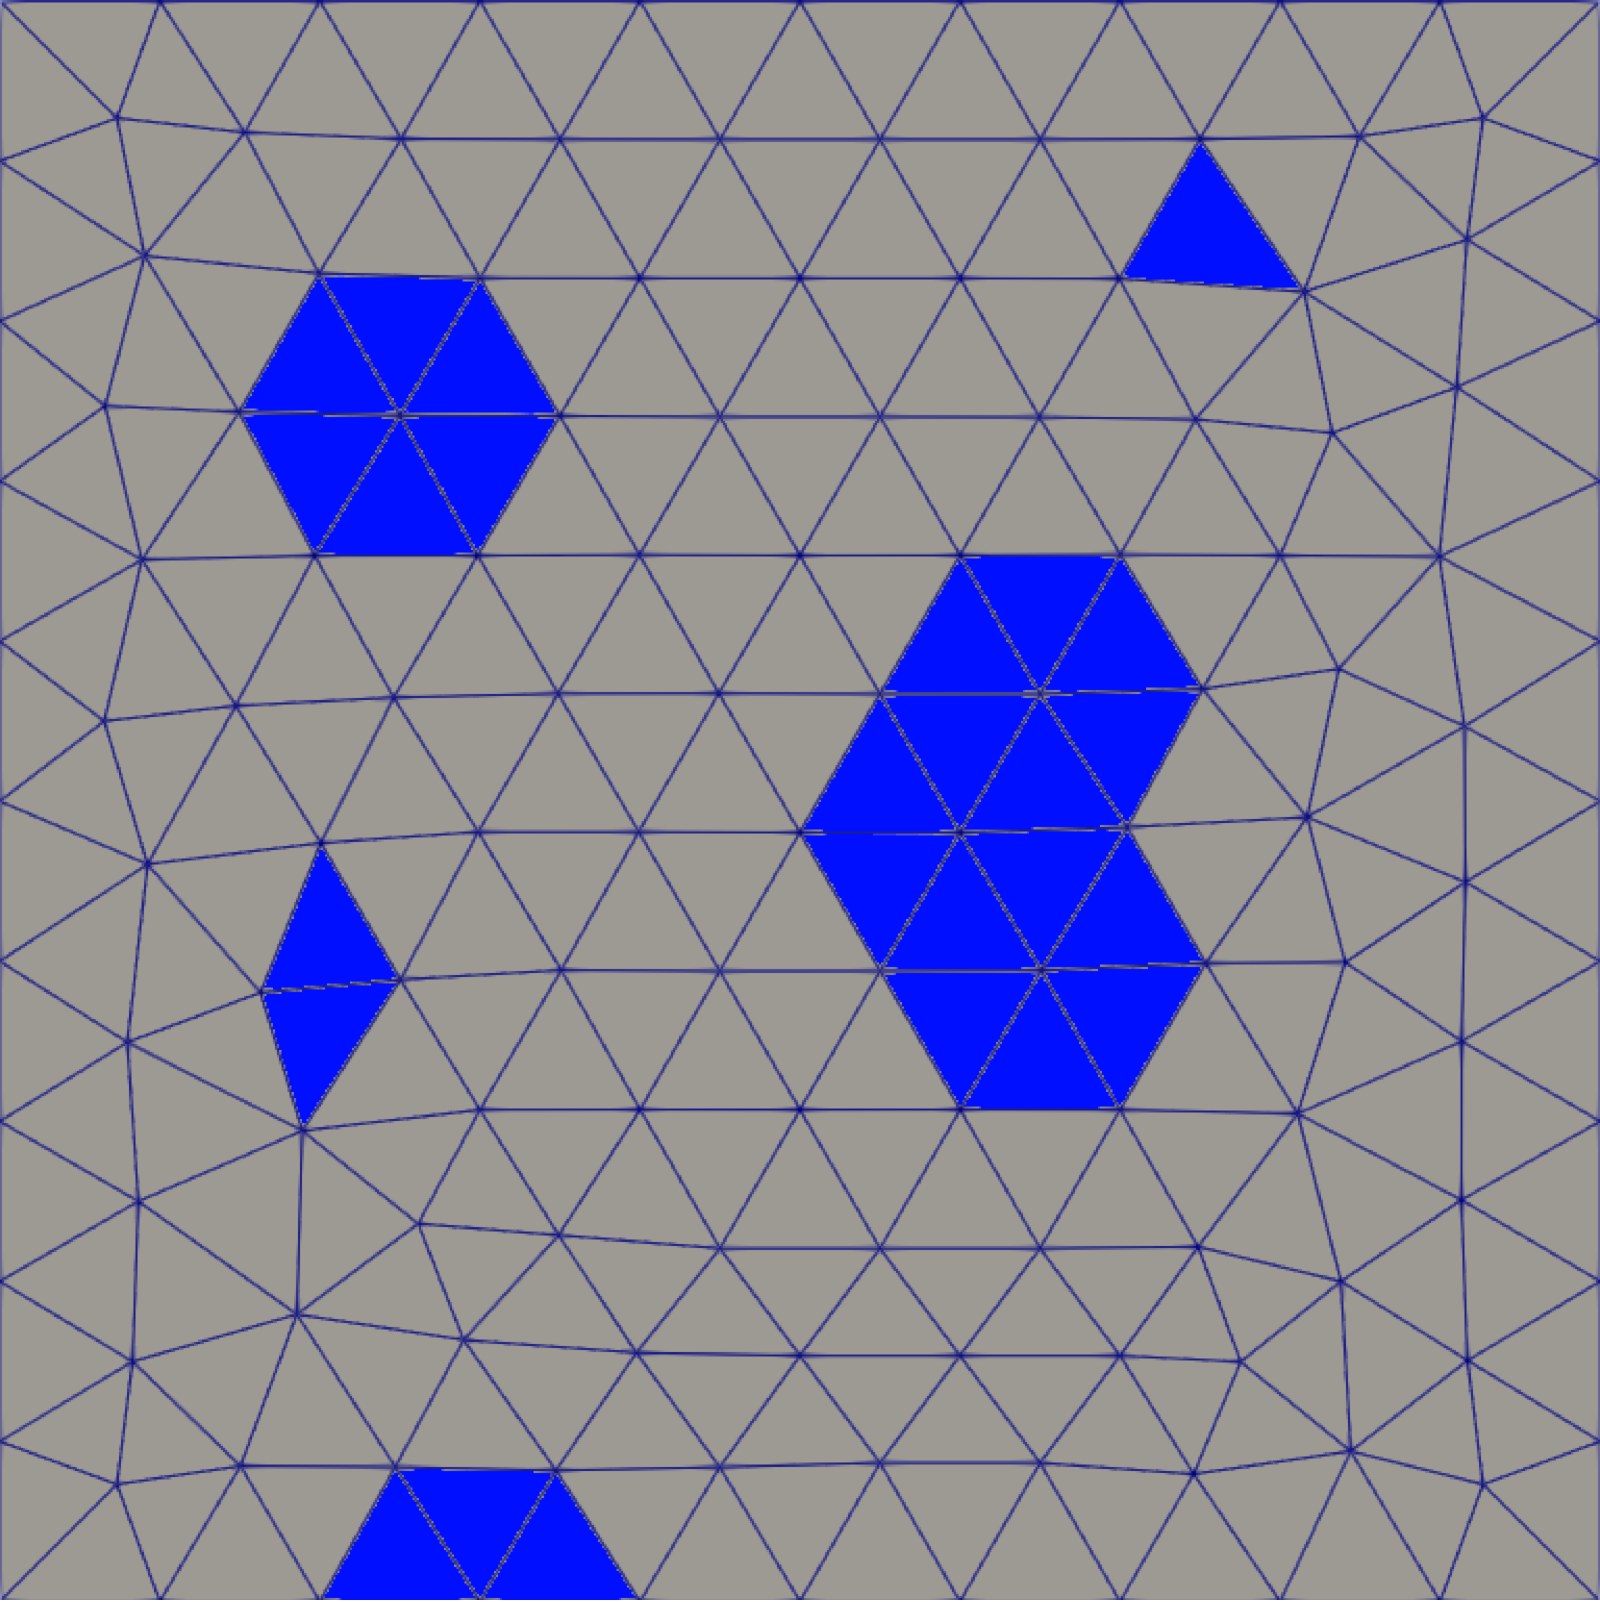
\includegraphics[width=\textwidth]{images/zone_singuliere_2.pdf}
    %\caption{Insertion de $E$.}
    %\label{fig:quad_carre}
\end{subfigure}
\caption{Illustration de la construction des zones singulières (en bleu). En rouge, les emplacements où l'une des conditions de la définition \ref{def:triangle_singulier} est vérifiée.}
\label{fig:zone_singuliere}
\end{figure}

Avec ces outils, nous sommes à présent en mesure de présenter notre proposition de représentation $\bar{u}_h$ sur $\Omega_h$ d'un champ de croix $\bar{u}$ défini sur $\Omega$. Pour tout $p\in\Omega_h$, nous définissons $\bar{u}_h$ de la manière suivante:\\

\begin{itemize}
\item[$\bullet$] si $p\in(S_h\backslash\mathbf{Z})\cap\partial Z$, alors $\bar{u}_h(p)$ est égale à la valeur nodale de $\bar{u}$ en $p$.\\%[-0.3cm]
\item[$\bullet$] si $p\in\Omega_h\backslash\mathbf{Z}$ alors il existe $T\in\mathcal{T}_h$ tel que $p\in T$ et $T$ n'est pas un triangle singulier. On pose alors:
$$
\left\{
\begin{array}{l}
\theta_1 = \theta_{\bar{u}_h}(s_1)\\\\
\theta_2 = \theta_1 + \delta\theta(\bar{u}_h(s_1),\bar{u}_h(s_2))\\\\
\theta_3 = \theta_2 + \delta\theta(\bar{u}_h(s_2),\bar{u}_h(s_3))
\end{array}
\right.
$$
où $s_1$, $s_2$ et $s_3$ sont les sommets du triangle $T$. La croix $\bar{u}_h(p)$ est alors donnée par:
$$
\left\{
\begin{array}{l}
\bar{u}_h(p)=\displaystyle\left\{\mathbf{R}\left(\theta_p+m\frac{\pi}{2}\right)(1,0)^t,~m\in\mathbb{Z}\right\},\\\\
\theta_p=\displaystyle\sum_{i\in\llbracket1, 3\rrbracket}\lambda_i\theta_i,
\end{array}
\right.
$$
avec $(\lambda_i)_{i\in\llbracket 1, 3\rrbracket}$ les coordonnées barycentriques de $p$ dans le triangle $T$. Autrement dit, ils vérifient $p=\sum_{i=1}^3\lambda_i s_i$ et $\sum_{i=1}^3\lambda_i=1$.\\
\item[$\bullet$] si $p\in\mathbf{Z}$ alors il existe une zone singulière $Z\subset\mathbf{Z}$ tel que $p\in Z$. On a alors:\\
\begin{itemize}
 \item si $p=S_Z$, alors $\bar{u}_h(p)=0$.\\
 \item sinon la croix $\bar{u}_h(p)$ est donnée par:
\begin{equation}
\label{eqn:etoilage}
\left\{
\begin{array}{l}
\bar{u}_h(p)=\bar{u}_h(\widetilde{p}),\\\\
\{\widetilde{p}\}=[S_Zp)\cap\partial Z.
\end{array}
\right.
\end{equation}
Notons que l'ensemble $[S_Zp)\cap\partial Z$ est bien réduit à un singleton puisque $Z$ est étoilé par rapport à $S_Z$.\\
\end{itemize}
\end{itemize}

\begin{remark}
La construction que nous avons exposé se base sur l'angle signé entre les croix des arêtes du maillage. Plus précisément, nous utilisons les variations du champ de croix le long des arêtes pour construire notre représentation en chaque point et pour évaluer les indices des points singuliers. Ainsi, lorsque cette variation angulaire n'est pas définie, notre représentation induit des points singuliers non isolés, comme nous le verrons dans le lemme \ref{lem:isolation_pt_sing}.
Pour palier ce désagrément, nous imposons dans toute la suite les conditions suivantes:\\
\begin{itemize}
 \item si on a $Z\subset\mathbf{Z}$ tel que $Z\cap\partial\Omega_h=\emptyset$, on doit avoir pour tout $p\in\partial Z\cap S_h$, $\bar{u}(p)\neq 0$ et pour tout arête $[s_1s_2]\subset\partial Z$, $\delta\theta(\bar{u}(s_1),\bar{u}(s_2))$ est défini.\\
 \item si on a $Z\subset\mathbf{Z}$ tel que $Z\cap\partial\Omega_h\neq\emptyset$, on impose $S_Z\in\partial\Omega_h$ et on doit avoir pour tout $p\in(\partial Z\cap S_h)\backslash\{S_Z\}$, $\bar{u}(p)\neq 0$ et pour tout arête $[s_1s_2]\subset\partial Z$, $\delta\theta(\bar{u}(s_1),\bar{u}(s_2))$ est défini.\\
\end{itemize}
Dans la pratique, il sera donc impératif de modifier un maillage qui ne satisfait pas ces contraintes. %La pertinence de ces contraintes prend tout son sens par la suite, avec l'approche de construction que nous proposons pour représenter $\bar{u}$ sur $\Omega_h$.
Étant donné que les points singuliers du champ de croix $\bar{u}$ sont isolés, on peut toujours satisfaire ces contraintes en affinant ou en modifiant localement (par exemple, par des opérations de retournement d'arêtes) un maillage qui ne satisfait pas ces contraintes.
\end{remark}

\subsection{Points singuliers, indice et ligne de champs}
\label{subsec:pt_sing_ind_lign_champ}

\subsubsection*{Points singuliers}

L'ensemble $\mathcal{S}_{\bar{u}_h}$, défini comme l'ensemble des points singuliers de $\bar{u}_h$, est constitué des points $p \in \Omega_h$ tels que $\bar{u}_h(p) = 0$. Par construction, les points singuliers de $\bar{u}_h$ sont isolés. C'est ce que montre le lemme suivant:

\begin{lemma}
\label{lem:isolation_pt_sing}
    Les points singuliers de $\bar{u}_h$ sont isolés.
\end{lemma}
\begin{proof}
    Soit $q$ un point singulier de $\bar{u}_h$. Par construction, il existe une zone singulière $Z_q\subset\mathbf{Z}$ tel que $q=S_Z$. Le point $q$ est isolé puisqu'on a $Z_q\cap\mathcal{S}_{\bar{u}_h}=\{q\}$. En effet, pour tout $p\in Z_q\backslash\{q\}$ on a $\bar{u}_h(p)=\bar{u}_h(\widetilde{p})$ où $\widetilde{p}$ est le point d'intersection entre la demi-droite $[qp)$ et le bord $\partial Z_q$ de $Z_q$. Il existe donc une arête $[s_1s_2]\in\mathcal{A}_h$ (de sommets $s_1$ et $s_2$) vérifiant $[s_1s_2]\subset\partial T_q$, contenant le point $\widetilde{p}$ et tel que $\delta\theta(\bar{u}_h(s_1), \bar{u}_h(s_2))$ est défini. Ainsi, pour tout $r\in [s_1s_2]$, on a $\bar{u}_h(r)\neq 0$. Il vient alors que $\bar{u}_h(\widetilde{p})\neq 0$ et par conséquent $p\notin \mathcal{S}_{\bar{u}_h}$. Autrement dit, $Z_q\cap\mathcal{S}_{\bar{u}_h}=\{q\}$.
\end{proof}
Dans la suite, étant donné $p\in\mathcal{S}_{\bar{u}_h}$ un point singulier de $\bar{u}_h$ nous désignerons par $Z_p$ la zone singulière contenant $p$.

\subsubsection*{Indice}
Examinons à présent l'indice des points singuliers de $\bar{u}_h$. Soit $p$ un point singulier de $\bar{u}_h$ avec $p\in\Omega_h\backslash\partial\Omega_h$. D'après le chapitre \ref{chap:theoritical} l'indice de $p$ est donné par:
$$
id_{\bar{u}_h}(p)=\frac{1}{2\pi}\int_0^1 d\theta^\gamma_{\bar{u}_h}=\frac{1}{2\pi}\sum_{\gamma_T\in\{\gamma\cap T,~T\in\mathcal{T}_h\}}\int_0^1 d\theta^{\gamma_T}_{\bar{u}_h}.
$$
où $\gamma$ est un chemin fermé paramétré sur $[0, 1]$ englobant $p$ et ne contenant aucun autre point singulier de $\bar{u}_h$. En pratique, nous calculerons l'indice d'un point $p$ en utilisant une paramétrisation $\gamma$ du bord $\partial Z_p$ de $Z_p$. De ce fait, l'indice du point $p$ s'écrit:
\begin{equation}
    \label{eqn:ind_int}
    id_{\bar{u}_h}(p)=\displaystyle\frac{1}{2\pi}\displaystyle\sum_{i=1}^{n_s}\left(\theta^\gamma_{\bar{u}_h}(s_{i+1})-\theta^\gamma_{\bar{u}_h}(s_i)\right)=\displaystyle\frac{1}{2\pi}\sum_{i=1}^{n_s}\delta\theta(\bar{u}_h(s_i),\bar{u}_h(s_{i+1})),
\end{equation}
où $(s_i)_{i\in\llbracket 1, n_s\rrbracket}=S_h\cap\partial Z_p$ désigne l'ensemble des sommets des triangles formant $Z_p$, privés du point $p$, et numérotés dans le sens positif avec $s_{n_s+1}:=s_1$.
Si $p\in\partial\Omega_h$ alors l'indice de $p$ est donné par:
\begin{equation}
    \label{eqn:ind_bord}
    id_{\bar{u}_h}(p)=\displaystyle\frac{1}{2\pi}\left[\pi-\widehat{p}+\displaystyle\sum_{i=1}^{n_s}\left(\theta^\gamma_{\bar{u}_h}(s_{i+1})-\theta^\gamma_{\bar{u}_h}(s_i)\right)\right]=\displaystyle\frac{1}{2\pi}\left[\pi-\widehat{p}+\displaystyle\sum_{i=1}^{n_s}\delta\theta(\bar{u}_h(s_i),\bar{u}_h(s_{i+1}))\right],
\end{equation}
où $\gamma$ dans ce cas est la paramétrisation de $\partial Z_p$ avec $\gamma(0)=\gamma(1)=p$ et $(s_i)_{i\in\llbracket 1, n_s\rrbracket}$ l'ensemble des sommets de $\Omega_h$ appartenant à $\partial Z_p\backslash\{p\}$ et numéroté dans le sens positif.

\begin{proposition}
\label{prop:ind_sing_zone}
Pour tout $p\in\Omega_h\backslash\partial\Omega_h$, on a:
$$
id_{\bar{u}_h}(p)\in\left\rrbracket-\frac{n_a}{4}, \frac{n_a}{4}\right\llbracket,
$$
où $n_a$ est le nombre d'arête de $\Omega_h$ inclut dans $\partial Z_p$.
\end{proposition}

\begin{proof}
Soit $p\in\Omega_h$. On sait que:
$$
id_{\bar{u}_h}(p)=\displaystyle\frac{1}{2\pi}\sum_{i=1}^{n_s}\delta\theta(\bar{u}_h(s_i),\bar{u}_h(s_{i+1})).
$$
Or pour tout $i\in\llbracket 1, n_s\rrbracket$, on a $\delta\theta(\bar{u}_h(s_i),\bar{u}_h(s_{i+1}))\in]-\frac{\pi}{4}, \frac{\pi}{4}[$. Autrement dit,
$$
\displaystyle\frac{1}{2\pi}\sum_{i=1}^{n_s}\delta\theta(\bar{u}_h(s_i),\bar{u}_h(s_{i+1}))\in\left]-\frac{n_s}{8}, \frac{n_s}{8}\right[.
$$
En outre, on sait que $4id_{\bar{u}_h}\in\mathbb{Z}$ et $n_s=n_a$. Par conséquent,
$$
id_{\bar{u}_h}(p)\in\left\rrbracket-\frac{n_a}{4}, \frac{n_a}{4}\right\llbracket.
$$
\end{proof}
Un corollaire direct de la proposition précédente est que si un point singulier est localisé à l'intérieur d'un triangle alors les seuls indices possibles pour ce point sont $-1/4, 0$ et $1/4$. Il vient donc que pour modéliser un point singulier d'ordre élevé, il est préférable qu'il soit localisé en un sommet du maillage. Puisque la position d'un point singulier est arbitraire dans une zone singulière, on peut donc en profiter pour placer les points singuliers sur des sommets ou encore effectuer un remaillage local permettant de capturer le point singulier sur un sommet comme dans \cite{jezdimirovic2021quad}.

\subsubsection*{Ligne de champs}
Nous abordons à présent la représentation des lignes de champs de $\bar{u}_h$ dans $\Omega_h$. Etant donné un point $p_0\in\Omega_h$ et un vecteur $\overrightarrow{u_0}\in\mathbb{R}^2$, la ligne de champ $SL_{\bar{u}_h}(p_0, \overrightarrow{u_0})$ d'origine $p_0$ est la courbe $S$ telle que :

\begin{enumerate}
\item il existe $\pi_{\bar{u}_h}^S:\Omega_h\longrightarrow\mathbb{R}^2$ une application telle que $\pi_{\bar{u}_h}^S(p_0)=\overrightarrow{u_0}$ et pour tout $p\in Im S$ il existe un voisinnage $V_p$ de $p$ tel que:
\begin{equation}
\pi_{\bar{u}_h}^S\in\mathcal{C}^1(V_p) \mbox{ et }  \forall q\in V_p, \pi_{\bar{u}_h}^S(q)\in \bar{u}_h(q),
\end{equation}
\item $S$ est une solution maximale dans $\Omega$ de l'équation différentielle
\begin{equation}
\frac{dS(t)}{dt}=\pi_{\bar{u}_h}^S(S(t)),t\in \mathbb{R} \text{ et }  S(0)=p_0.
\label{eqn:stream_equation}
\end{equation}
\end{enumerate}

\subsection{Lien entre $\bar{u}$ et $\bar{u}_h$}
\label{Lien_u_u_h}

Dans cette section, nous procédons à une comparaison entre le champ de croix $\bar{u}$ et sa représentation discrète $\bar{u}_h$. L'objectif est de mieux comprendre l'adéquation entre ces deux formulations et d'évaluer la précision de l'approximation $\bar{u}_h$ par rapport au champ continu $\bar{u}$.

\paragraph{Points singuliers:}
Une conséquence de la représentation du champ de croix que nous avons présentée est que les points singuliers de $\bar{u}$ ne correspondent pas aux points singuliers de $\bar{u}_h$ ($\mathcal{S}_{\bar{u}}\neq\mathcal{S}_{\bar{u}_h}$). Par exemple, sur la figure \ref{fig:eclatement_point_sing}, nous avons un champ de croix contenant un point singulier d'indice $1$ que nous représentons sur un maillage triangulaire. On observe alors la présence d'une multitude de points singuliers d'indice $1/4$ et d'indices $-1/4$, localisés dans divers triangles (voir la proposition \ref{prop:ind_sing_zone}).

\begin{figure}[htpb]
\centering
\begin{subfigure}[b]{0.495\textwidth}
    \centering
    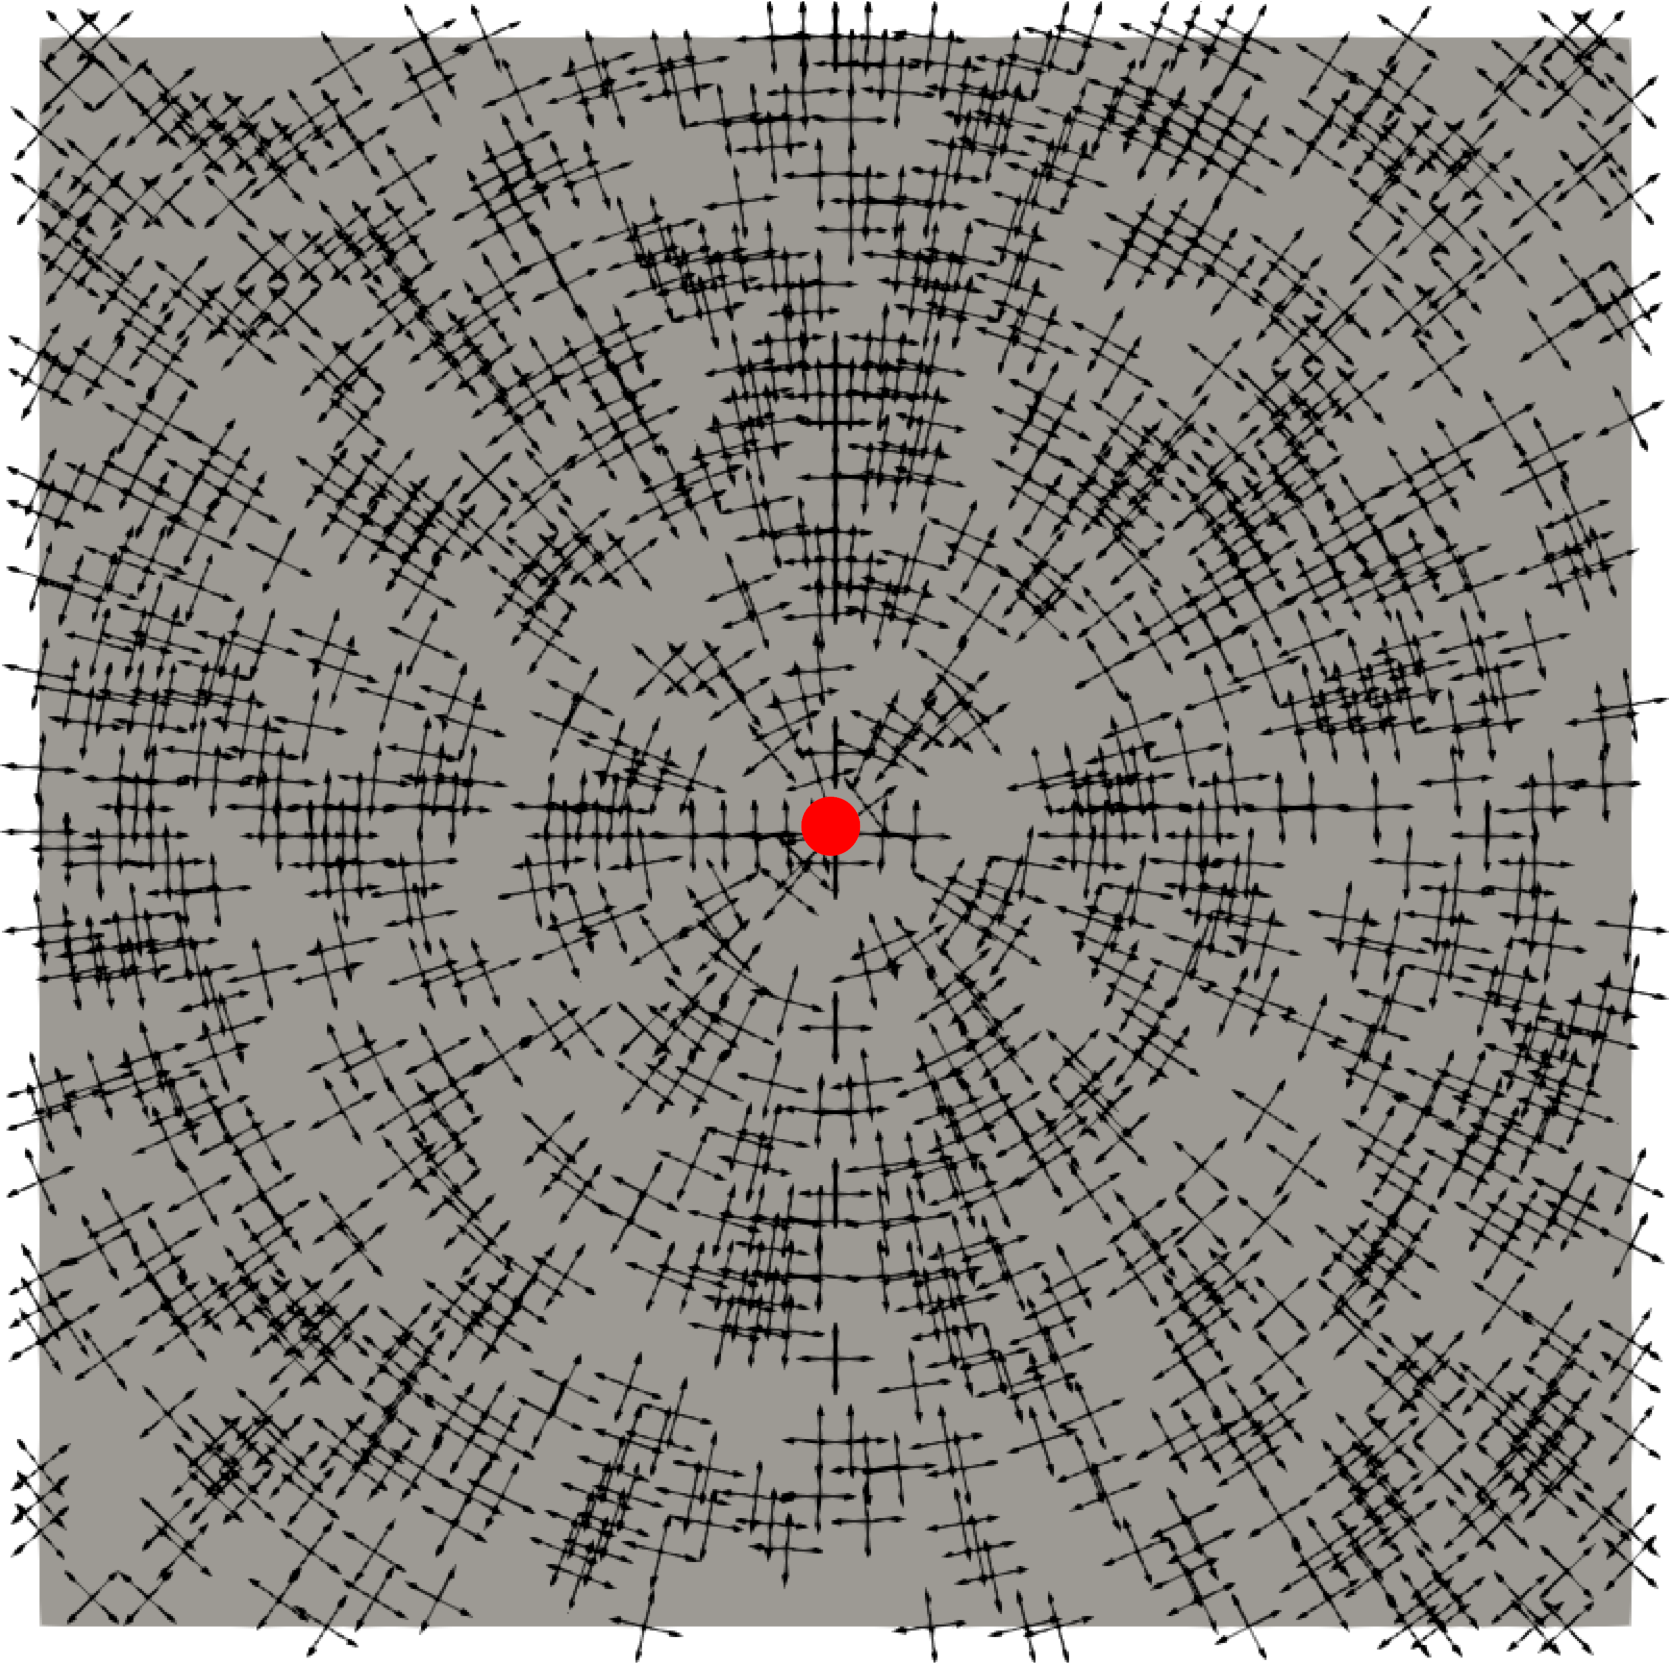
\includegraphics[width=\textwidth]{images/u_sing.pdf}
    \caption{Champ de croix $\bar{u}$.}
\end{subfigure}
\hfill
\begin{subfigure}[b]{0.495\textwidth}
    \centering
    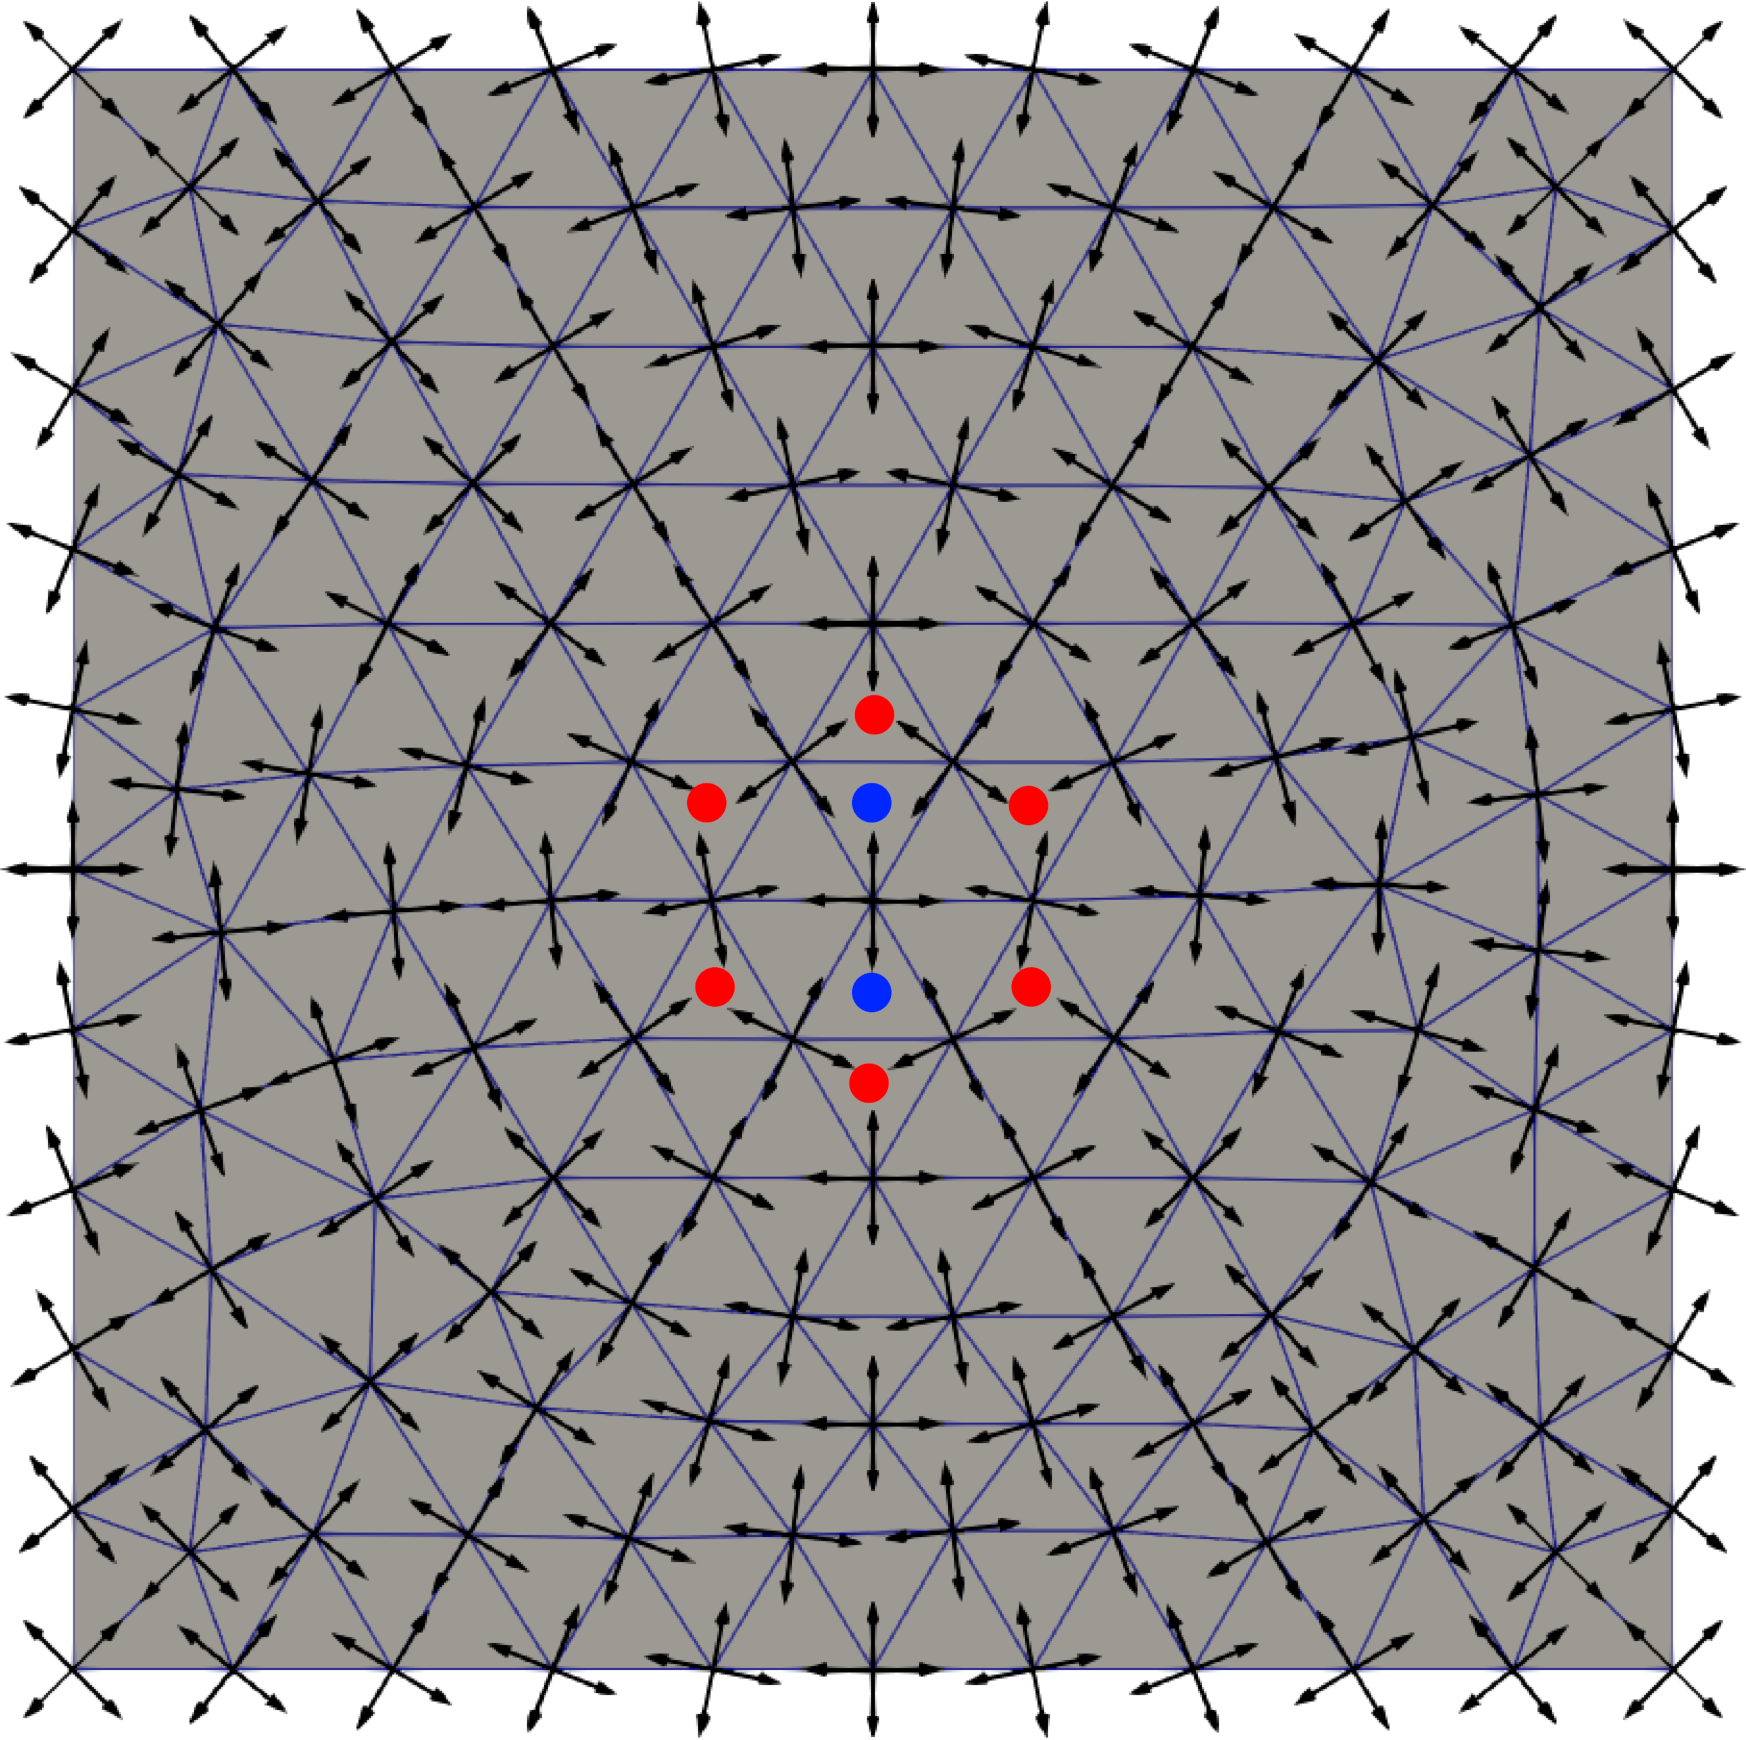
\includegraphics[width=\textwidth]{images/u_h_sing.pdf}
    \caption{Champ de croix $\bar{u}_h$.}
\end{subfigure}
  \caption{Comparaison de la localisation des points singuliers entre $\bar{u}$ et $\bar{u}_h$.}
  \label{fig:eclatement_point_sing}
\end{figure}

\paragraph{Singularités d'ordre supérieur:} Cependant, il est possible de représenter des singularités d'ordre supérieur (dont la valeur absolue de l'indice est supérieure à $1/4$) en exploitant la méthode des zones singulières présentée précédemment lors de la construction de la représentation d'un champ de croix sur un maillage triangulaire. Pour ce faire, on réuni des triangles dans un voisinage donné en tant que zone singulière, au sein de laquelle on modifie le champ de croix en utilisant l'équation \eqref{eqn:etoilage}. Par la suite, on sélectionne un point arbitraire dans la zone singulière pour représenter le point singulier unique de cette partie du domaine, et son indice correspond à la somme des indices de tous les points singuliers présents dans les triangles (ceux ayant formé la zone singulière) avant la modification locale du champ de croix (voir la proposition \ref{prop:stream_from_interior_sing}).

Il est essentiel de souligner que dans cette opération, le maillage demeure inchangé. En pratique, on conserve simplement en mémoire les triangles constituant les zones singulières ainsi que le point choisi comme singulier dans la zone. La valeur du champ de croix est ensuite obtenue (si nécessaire) en un point en appliquant l'équation \eqref{eqn:etoilage}.

\paragraph{Convergence:}
Soit $\eta$ une fonction définie sur $\Omega$ et $\eta_h$ sa représentation en éléments finis définie sur $\Omega_h$. Notons que $\bar{\Omega}$ ne correspond pas nécessairement à la réunion des triangles de $\Omega_h$ (voir figure \ref{fig:Omega_vs_Omega_h}). Par conséquent, les supports de $\eta$ et de $\eta_h$ ne coïncident pas. Pour comparer ces deux fonctions, nous nous appuyons sur les travaux de \cite{dziuk1988finite} en introduisant une opération d'extension, appelée \emph{lift}, qui permet d'étendre $\eta_h$ sur $\Omega$ et que nous notons $[\mathbf{L}_{\Omega_h}^{\Omega}\eta_h]$.

Supposons que $\Omega$ peut être représenté globalement par une fonction de distance orientée $d$ définie sur un sous-ensemble ouvert $U$ de $\mathbb{R}^2$
\[
\Omega=\{x\in U,~d(x)=0\},
\]
où $d$ est dans $\mathcal{C}^{k,\alpha}(U)$, $\nabla d\neq 0$ ($k\in\mathbb{N}\cup\{0\},~0\leq\alpha\leq 1$). Le lift $[\mathbf{L}_{\Omega_h}^{\Omega}\eta_h]$ est alors défini par :
\begin{equation}
\eta_h(p)=[\mathbf{L}_{\Omega_h}^{\Omega}\eta_h](p-d(p)n(p))\mbox{ pour tout }p\in\Omega_h,
\end{equation}
où $n(p)$ est la normale sortante en $p$. Il résulte des travaux de \cite{dziuk1988finite} que $[\mathbf{L}_{\Omega_h}^{\Omega}\eta_h]$ converge vers $\eta$, et que l'erreur de représentation de la géométrie (d'ordre 2) est négligeable par rapport à l'erreur d'approximation du schéma numérique.


\begin{figure}[!h]
  \centering
  \includegraphics[scale=0.5]{images/Omega_vs_Omega_h.pdf}
  \caption{Comparaison de $\Omega$ et $\Omega_h$.}
  \label{fig:Omega_vs_Omega_h}
\end{figure}


Nous cherchons à appliquer ces résultats pour comparer le champ de croix $\bar{u}_h$ défini sur $\Omega_h$ avec le champ de croix $\bar{u}$ défini sur $\Omega$. On considère qu'une suite de champs de croix converge vers un autre champ de croix lorsque les champs d'angles associés convergent les uns vers les autres.

Pour tout élément $T\in\mathcal{T}_h$ avec $T$ non-singulier, la construction assure l'existence d'une fonction $m:T\longrightarrow \mathbb{Z}$ telle que $\theta_{\bar{u}_h}+m\pi/2$ soit linéaire dans $T$. En utilisant les résultats de \cite{dziuk1988finite}, on en déduit que $[\mathbf{L}_{\Omega_h}^{\Omega}\theta_{\bar{u}_h}]$ tend vers $\theta_{\bar{u}}$ sur $\Omega\backslash\cup_{Z\in\mathbf{Z}}Z$ lorsque $h$ tend vers $0$. Lorsque $h$ tend vers $0$, le diamètre des triangles du maillage diminue, ce qui entraîne une réduction de la taille des zones singulières $Z$ pour tout $Z\in\mathbf{Z}$. Par conséquent, lorsque $h$ tend vers $0$, le champ scalaire $[\mathbf{L}_{\Omega_h}^{\Omega}\theta_{\bar{u}_h}]$ converge vers $\theta_{\bar{u}}$ sur $\Omega$. Plus précisement, on a:
$$||\theta_{\bar{u}}-[\mathbf{L}_{\Omega_h}^{\Omega}\theta_{\bar{u}_h}]||_{L^2(\Omega)}\leq ch,$$
où $c$ est une constante. Ainsi, le lift $[\mathbf{L}_{\Omega_h}^{\Omega}\bar{u}_h]$ sur $\Omega$ du champ de croix $\bar{u}_h$ converge vers le champ de croix $\bar{u}$ sur $\Omega$ lorsque $h$ tend vers $0$.

\section{Partitionnement de $\partial\Omega_h$}
\label{sec:partitionnement_omega_h}

L'adaptation de l'algorithme de partitionnement \ref{alg:algo_main} au maillage $\Omega_h$ est donné par l'algorithme \ref{alg:discr_algo_main}. On considère que l'algorithme a convergé si les séparatrices ne convergent pas vers un cycle limite. Dans la suite, nous examinons maintenant en détail certaines étapes de cet algorithme.

%\vspace{0.2cm}
\RestyleAlgo{ruled}
\begin{algorithm}[h!]
\renewcommand{\algorithmcfname}{Algorithme}%
\SetAlgoLined
\Entree{$\Omega_h$ un maillage triangulaire, champ de croix $\bar{u}_h$}
\Sortie{Partition de $\Omega_h$ en ensembles de régions}
\vspace{0.2cm}
1.\quad Identification des points singuliers du champ de croix\\[0.2cm]
2.\quad Détermination du nombre de séparatrices pour chaque point singulier\\[0.2cm]
3.\quad Intégration des séparatrices\\[0.2cm]
4.\quad Identification des régions\\[0.2cm]
\caption{Partitionnement $\Omega_h$}
\label{alg:discr_algo_main}
\end{algorithm}
%\vspace{0.2cm}

\subsection{Recherche de points singuliers}

Par construction, les points singuliers du champ de croix $\bar{u}_h$ se situent soit aux sommets du maillage $\Omega_h$, soit sur une arête, soit à l'intérieur d'un triangle. Ces points singuliers coïncident exactement avec les points $S_Z$ où $Z\subset\mathbf{Z}$, tels que par construction. Une fois localisés, on peut facilement calculer leur indice grâce aux formules \ref{eqn:ind_int} ou \ref{eqn:ind_bord} en fonction de leur emplacement.

\begin{remark}
L'emplacement d'un point singulier $p$ dans $Z_p$ n'est pas fixé de manière absolue. La proposition \ref{prop:stream_from_interior_sing} indique qu'il est possible de faire correspondre ce point singulier à tout point à l'intérieur de $Z_p$, moyennant une modification du champ dans $Z_p$ comme spécifié dans plus haut.

En suivant cette logique, il est envisageable de substituer un groupe de singularités par un unique point singulier. Pour ce faire, il suffit de redéfinir l'ensemble $Z_p$ de manière à ce qu'il englobe tous les points singuliers que l'on souhaite regrouper avec $p$. Cette approche est bénéfique car elle permet de traiter les points singuliers situés trop près les uns des autres, évitant ainsi des séparatrices très rapprochées qui favoriseraient un partitionnement non homogène.
\end{remark}

\subsection{Construction des séparatrices}
\label{sub:sepa_constr}

Une fois les points singuliers de $\bar{u}_h$ identifiés, nous procédons à la création des séparatrices sur $\Omega_h$. Cette étape comprend le calcul du nombre de séparatrices à assigner à chaque point singulier, la détermination des directions initiales pour chaque séparatrice, ainsi que l'intégration de ces séparatrices.

\paragraph{Nombre de séparatrices:} Si $p$ est un point singulier de $\bar{u}_h$, alors le nombre de séparatrices $N_s(p)$ associées à $p$ est donné par:
\begin{equation}
    N_s(p) =
    \left\{
    \begin{array}{ll}
    4-4id_{\bar{u}_h}(p) & \mbox{ si } p\in\Omega_h\backslash\partial\Omega_h\\[0.3cm]
    3-4id_{\bar{u}_h}(p) & \mbox{ si } p\in\partial\Omega_h
    \end{array}
    \right.
\end{equation}

\begin{figure}[!h]
\centering
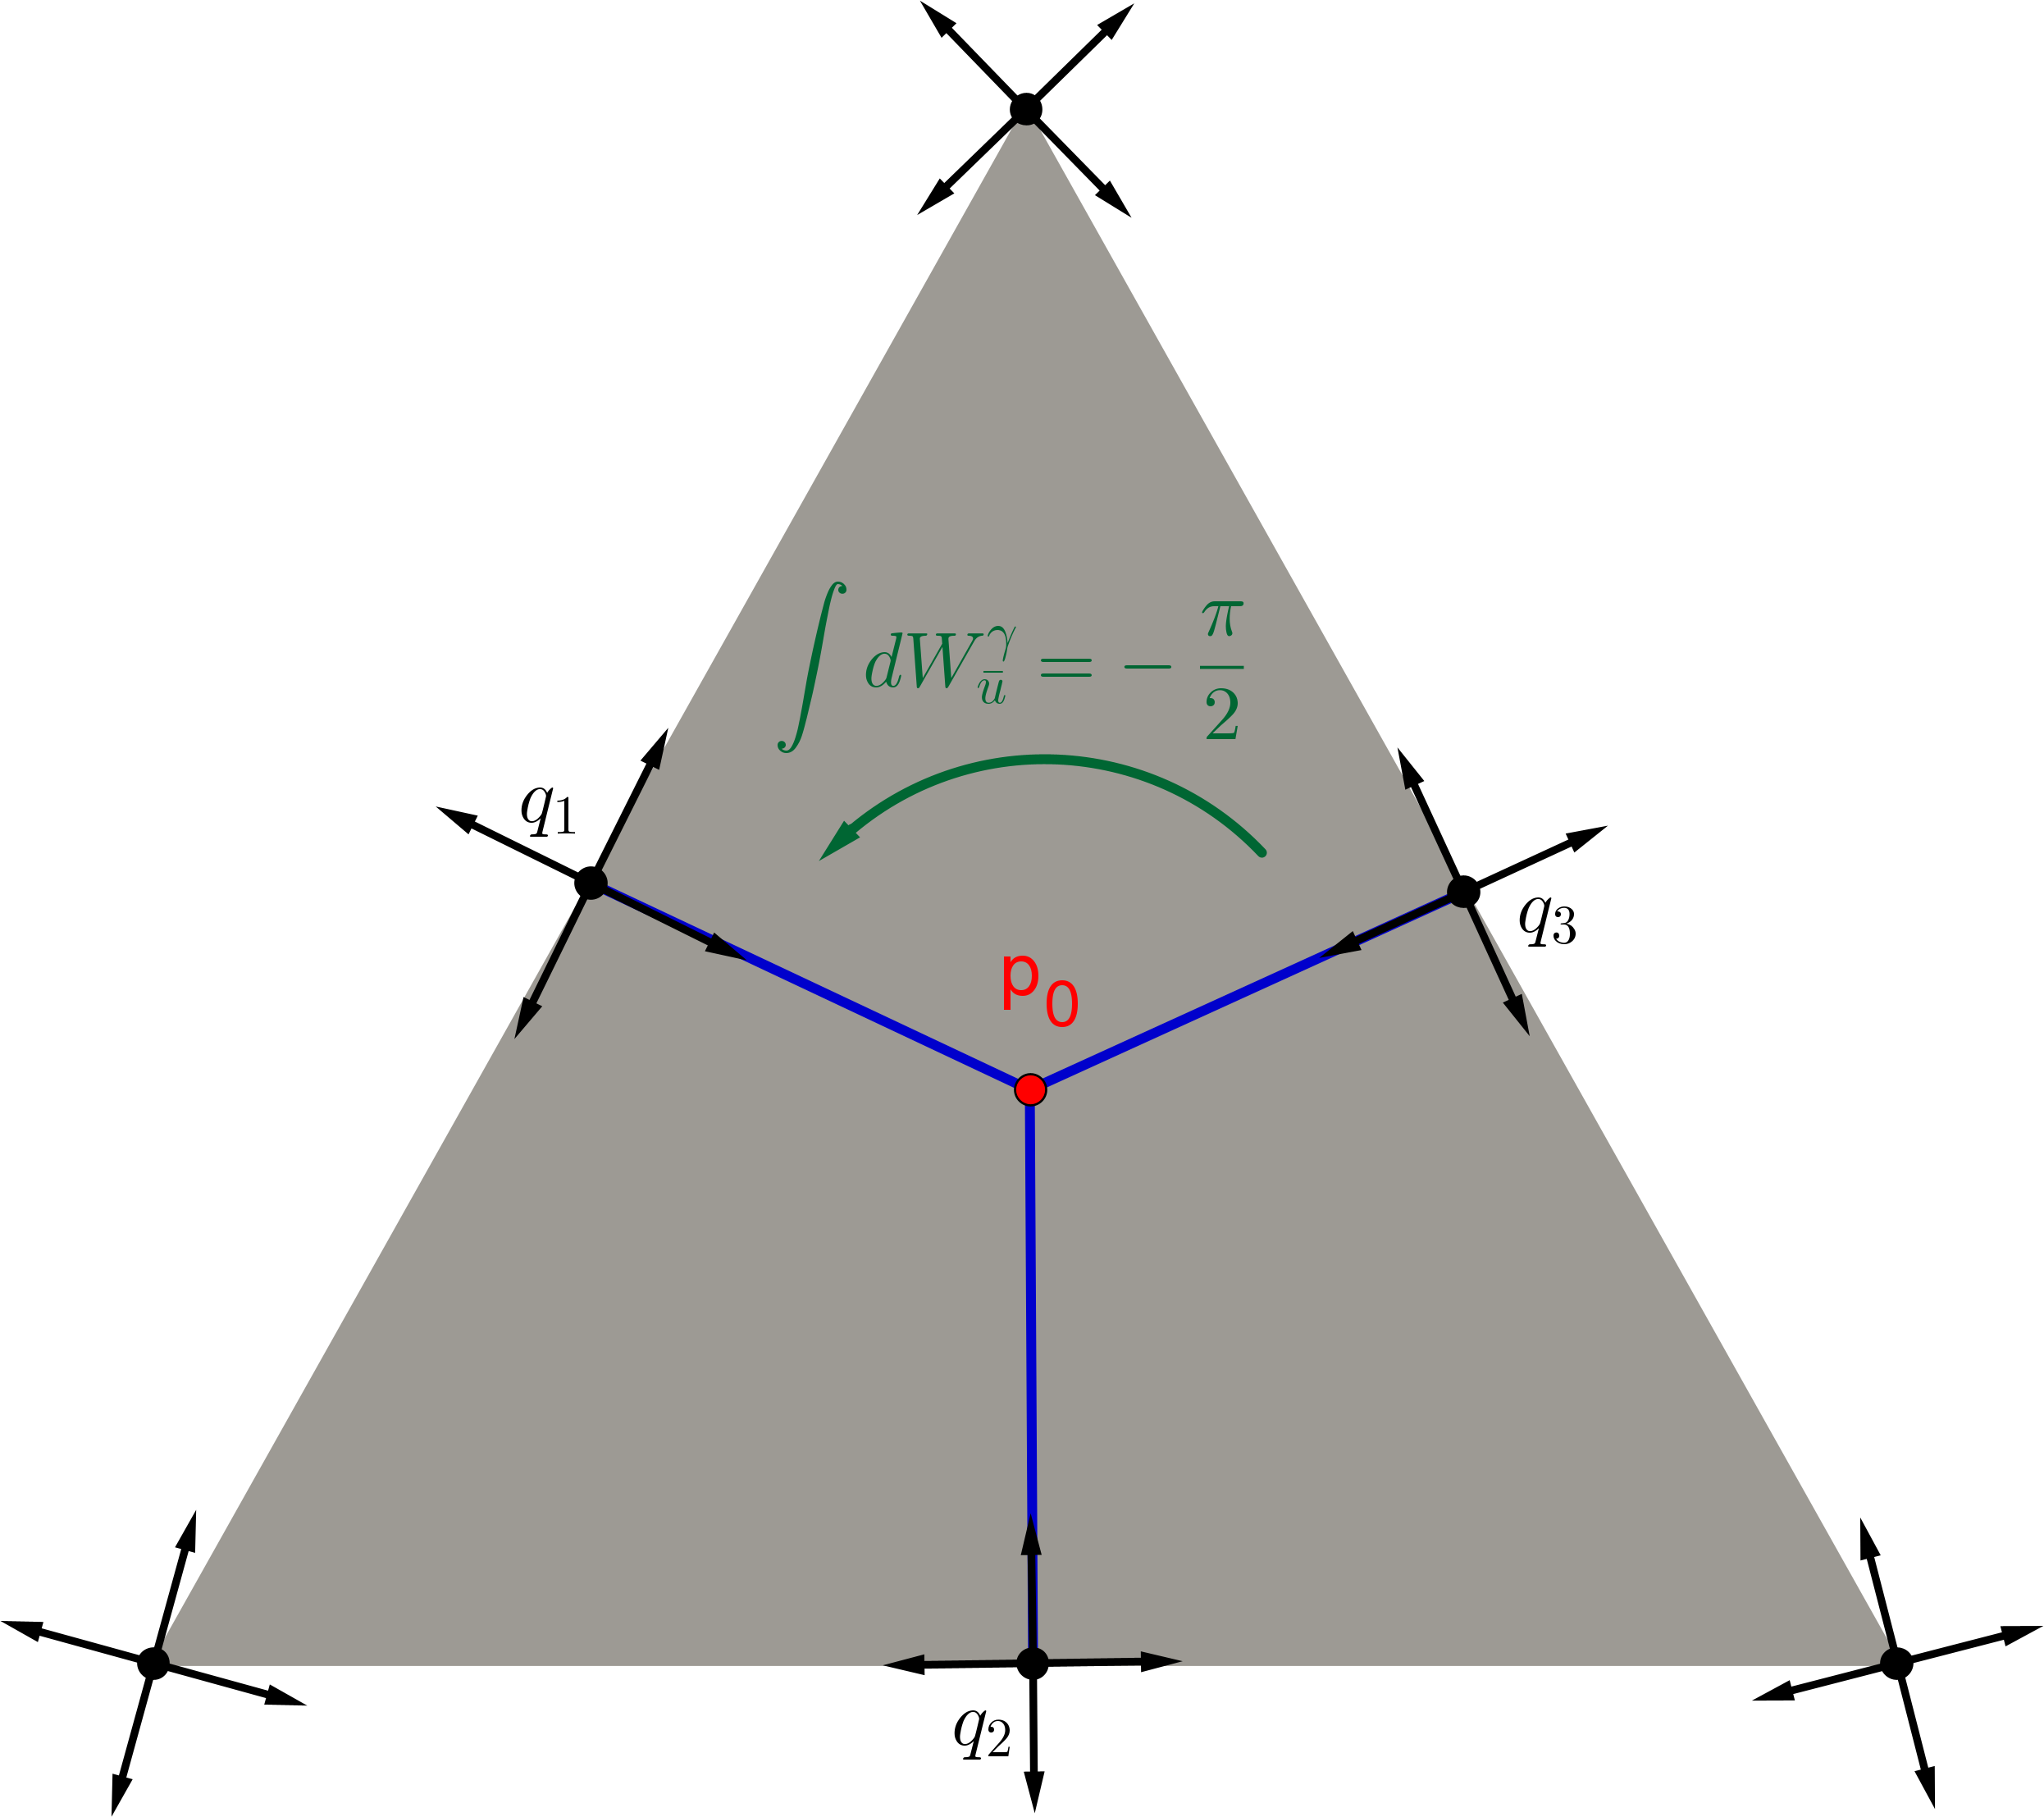
\includegraphics[scale=0.755]{images/triangle separatrices 3.png}
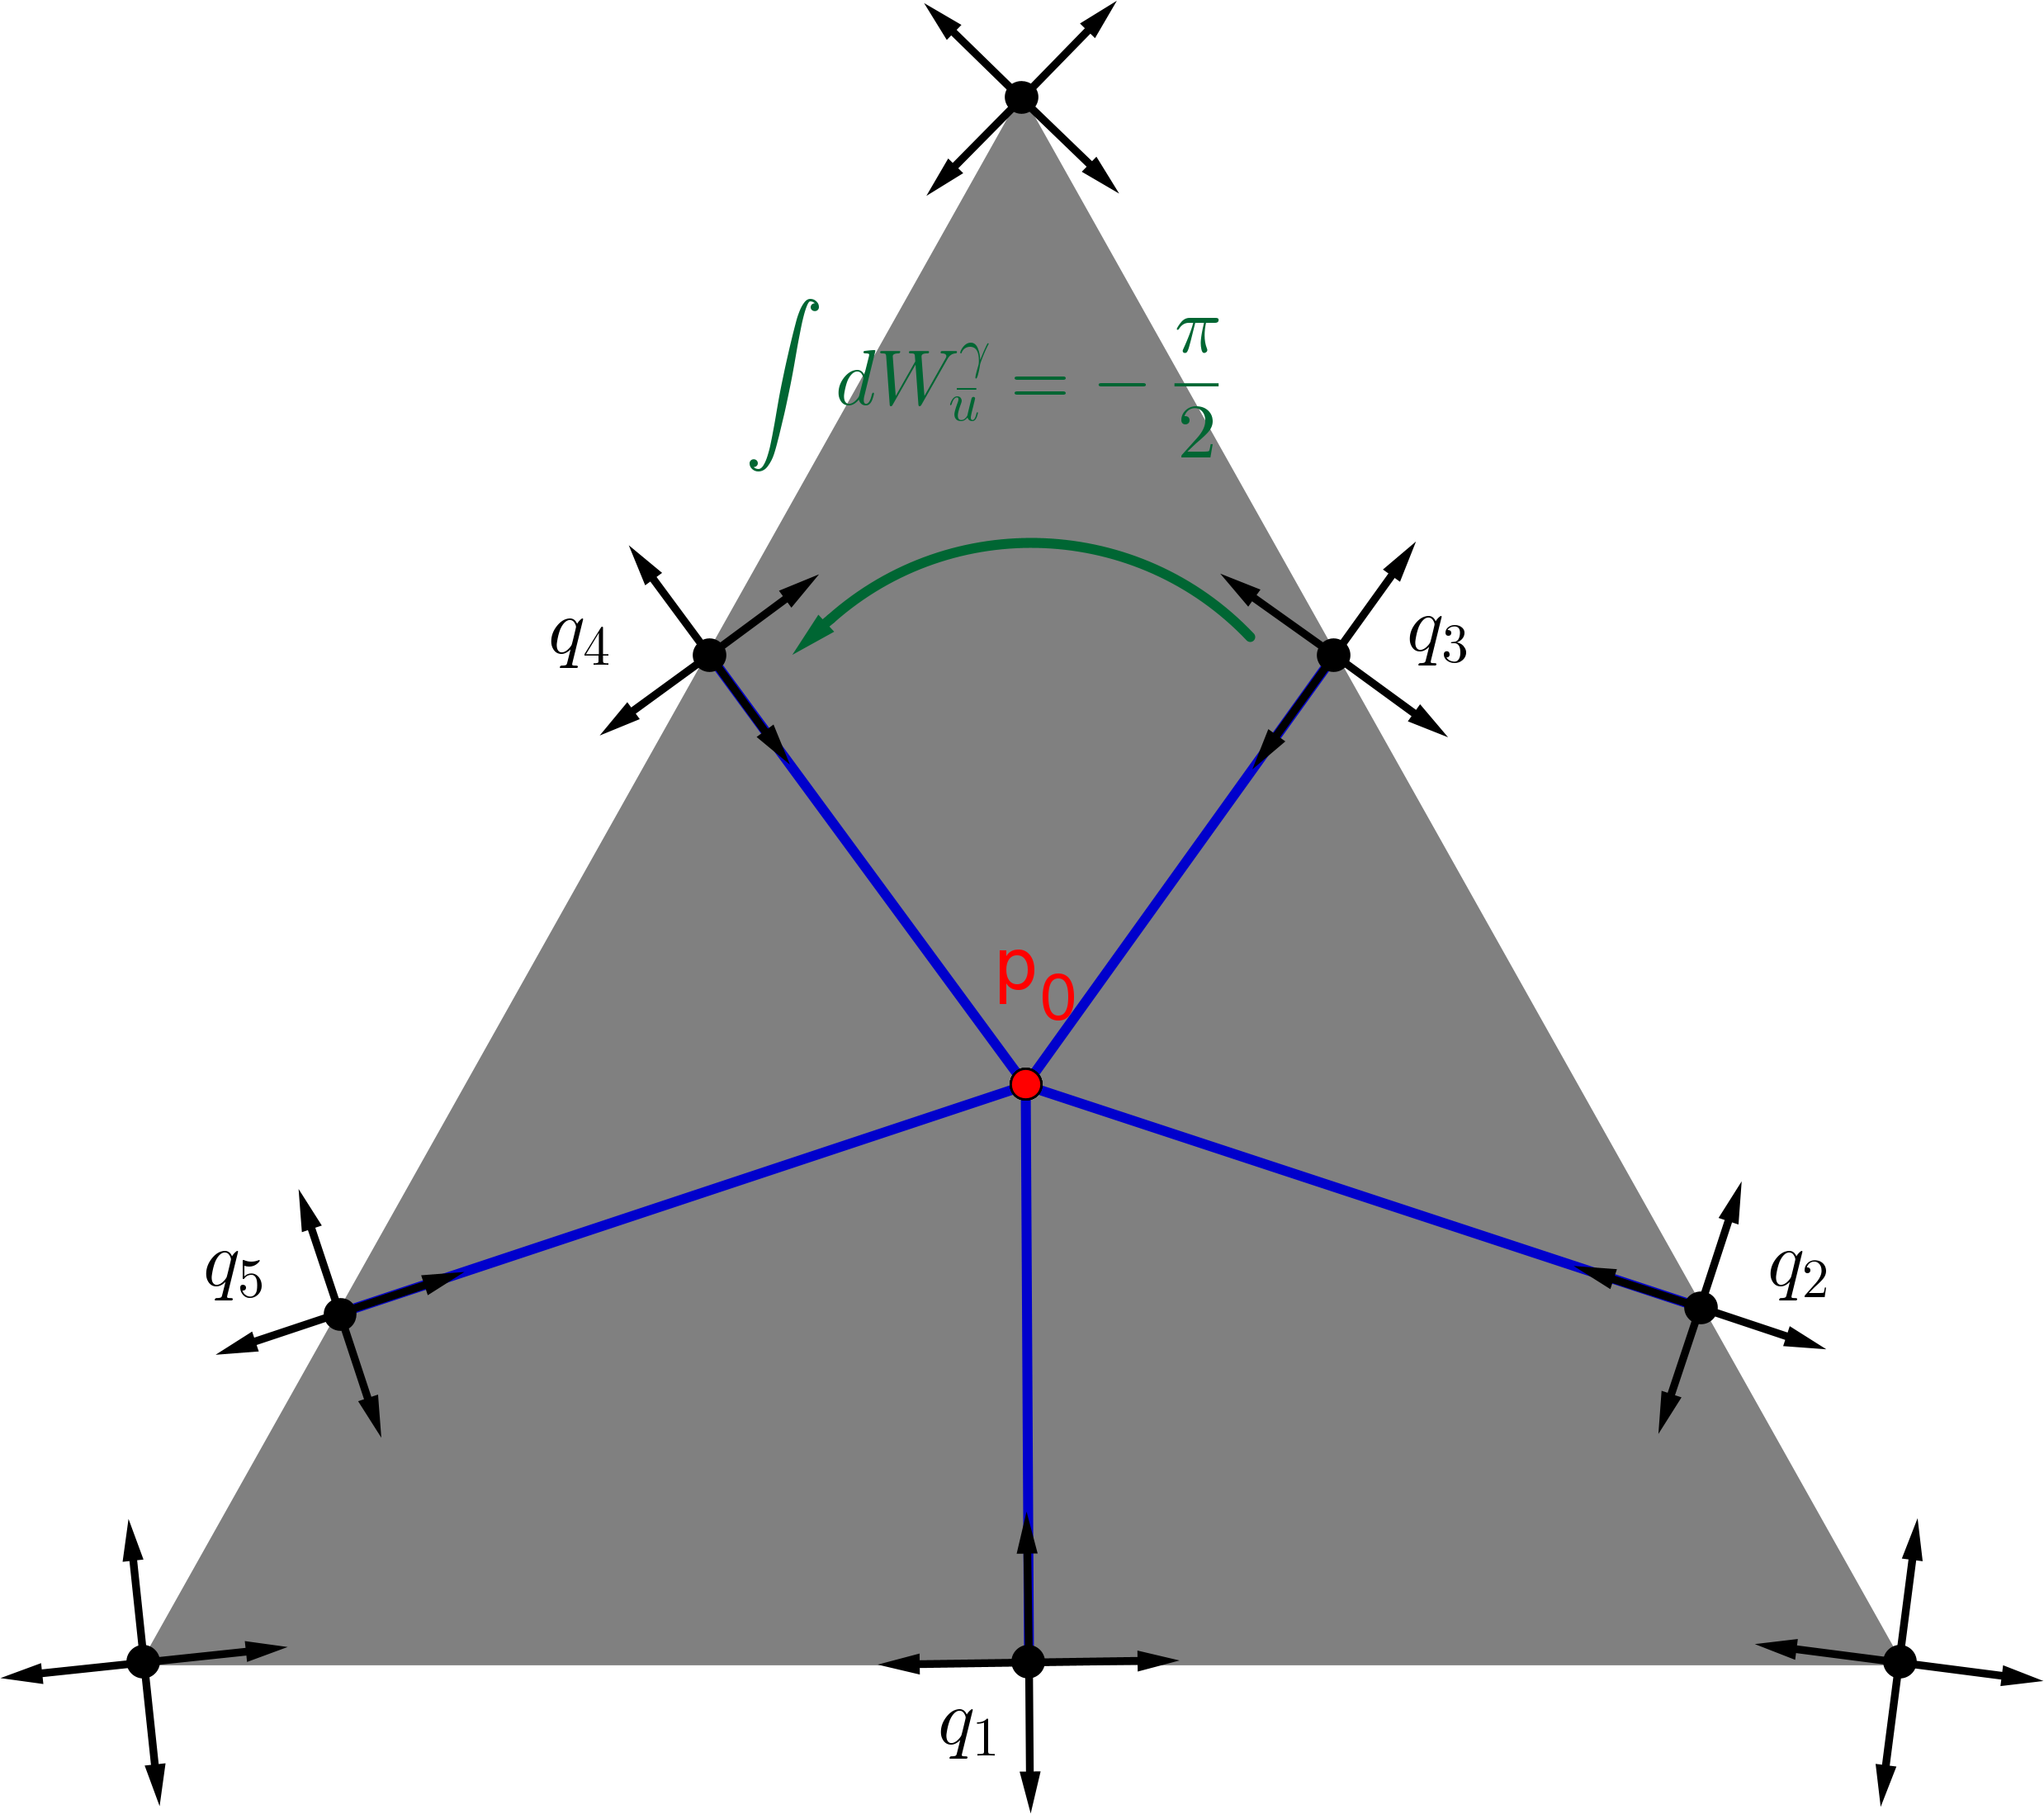
\includegraphics[scale=0.755]{images/triangle separatrices 5.png}
\caption{Illustration de l'initialisation de séparatrices à partir d'un point singulier d'indice 1/4 et d'un point singulier d'indice -1/4.}
\label{fig:init_streams_int}
\end{figure}

\begin{figure}[!h]
\centering
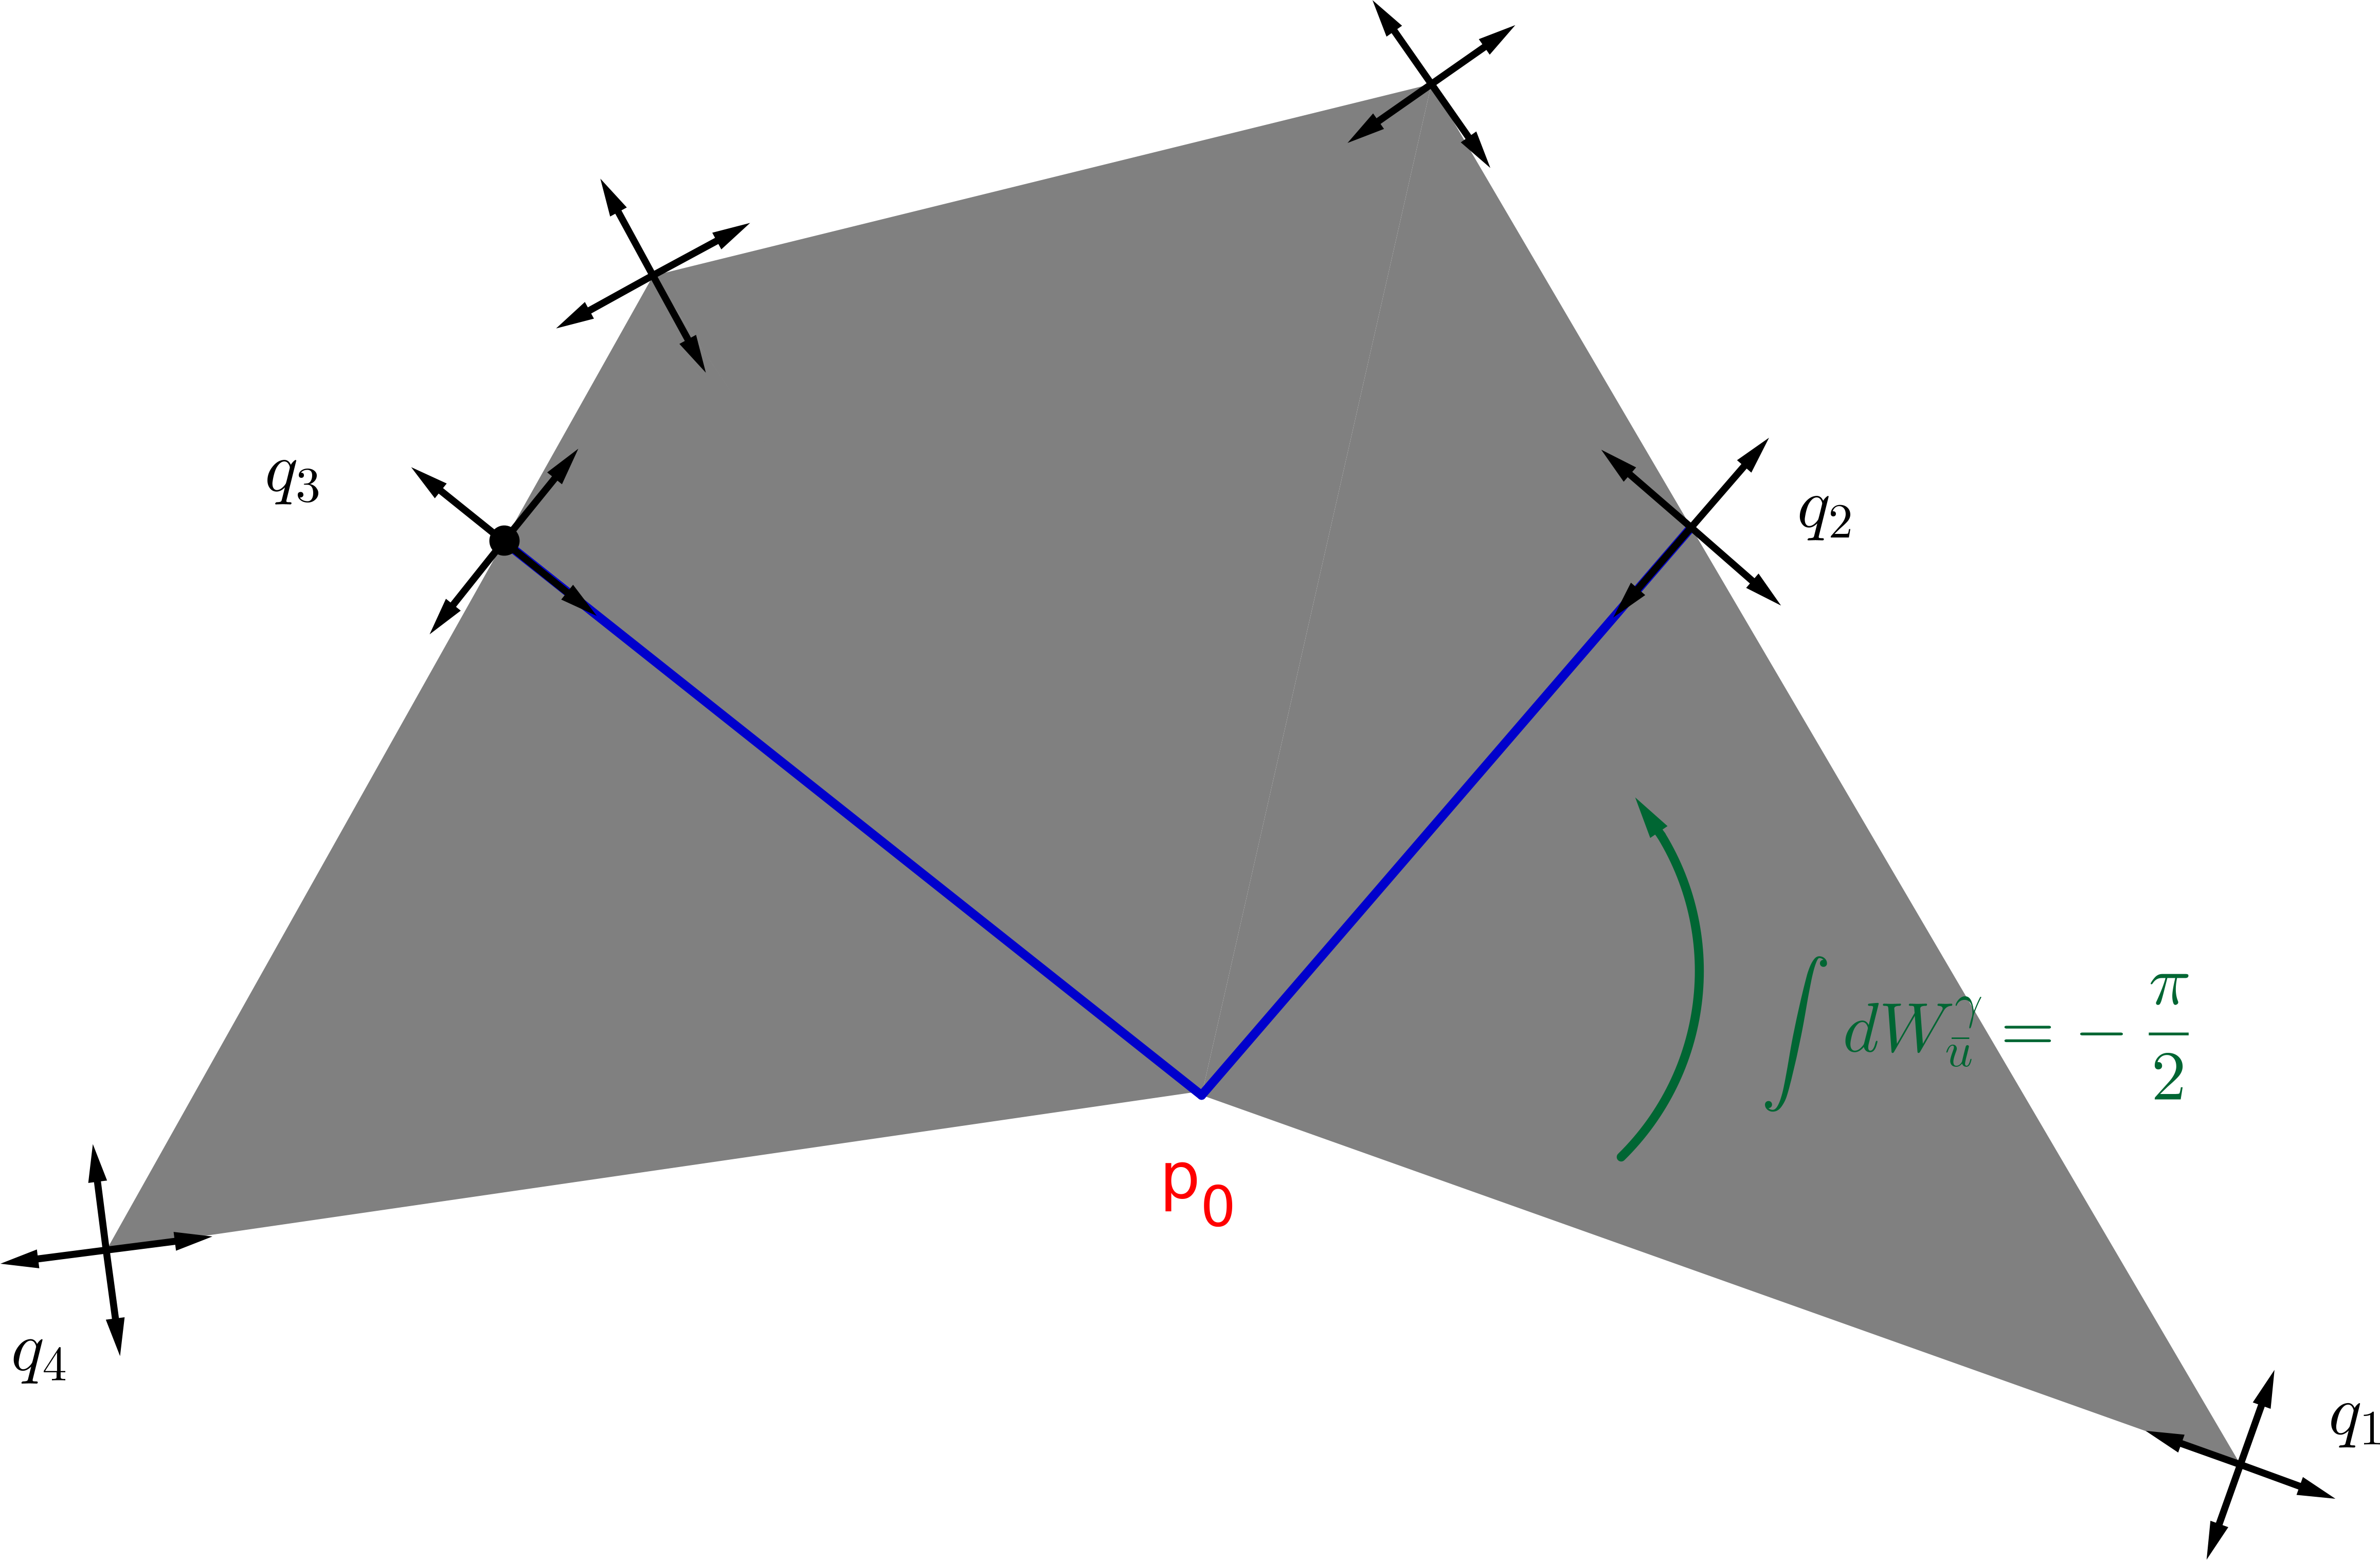
\includegraphics[scale=0.755]{images/triangle separatrices bord.png}
\caption{Illustration de l'initialisation de séparatrices à partir d'un point singulier de bord d'indice -1/4.}
\label{fig:init_streams_bord}
\end{figure}

\paragraph{Initialisation des séparatrices:}

Soit $p_0\in\mathcal{S}_{\bar{u}_h}\backslash\partial\Omega_h$. Étant donné que $\bar{u}_h$ s'annule en $p_0$, notre première étape consiste à déterminer les orientations initiales des séparatrices. Les directions initiales des séparatrices émanant de $p_0$ sont données par les vecteurs $\overrightarrow{p_0q_i}$, $i\in\llbracket 1, N_s(p_0) \rrbracket$ où la suite de points $(q_i)_{i\in\llbracket 1, N_s(p_0)\rrbracket}\subset\partial Z_{p_0}$ est construite de la manière suivante (voir figure \ref{fig:init_streams_int}):\\
\begin{itemize}
    \item[$\bullet$] le premier point $q_1$ est tout point de $\partial Z_{p_0}$ tel que $\overrightarrow{p_0q_1}.\|\overrightarrow{p_0q_1}\|^{-1}\in\bar{u}_h(q_1)$\\
    \item[$\bullet$] soit $t_1\in[0, 1]$ tel que $\gamma(t_1)=q_1$. Pour tout $i\in\llbracket 2, N_s(p_0)\rrbracket$, on a:
    $$
    q_i=\gamma(t_i)\mbox{ avec }\int_{t_{i-1}}^{t_i}dW_{p_0}^\gamma=-\frac{\pi}{2},
    $$
    où $\gamma$ est une paramétrisation de $\partial Z_{p_0}$ sur $[0, 1]$ dans le sens positif et la fonction $W^\gamma_{p_0}$ est donné pour tout $t\in[0, 1]$ par:
    $$
    W_{p_0}^\gamma(t)=\theta^\gamma_{\bar{u}_h}(t)-\arg \overrightarrow{p_0\gamma(t)}.
    $$
\end{itemize}


\begin{figure}[htpb]
\centering
\begin{subfigure}[b]{0.7\textwidth}
    \centering
    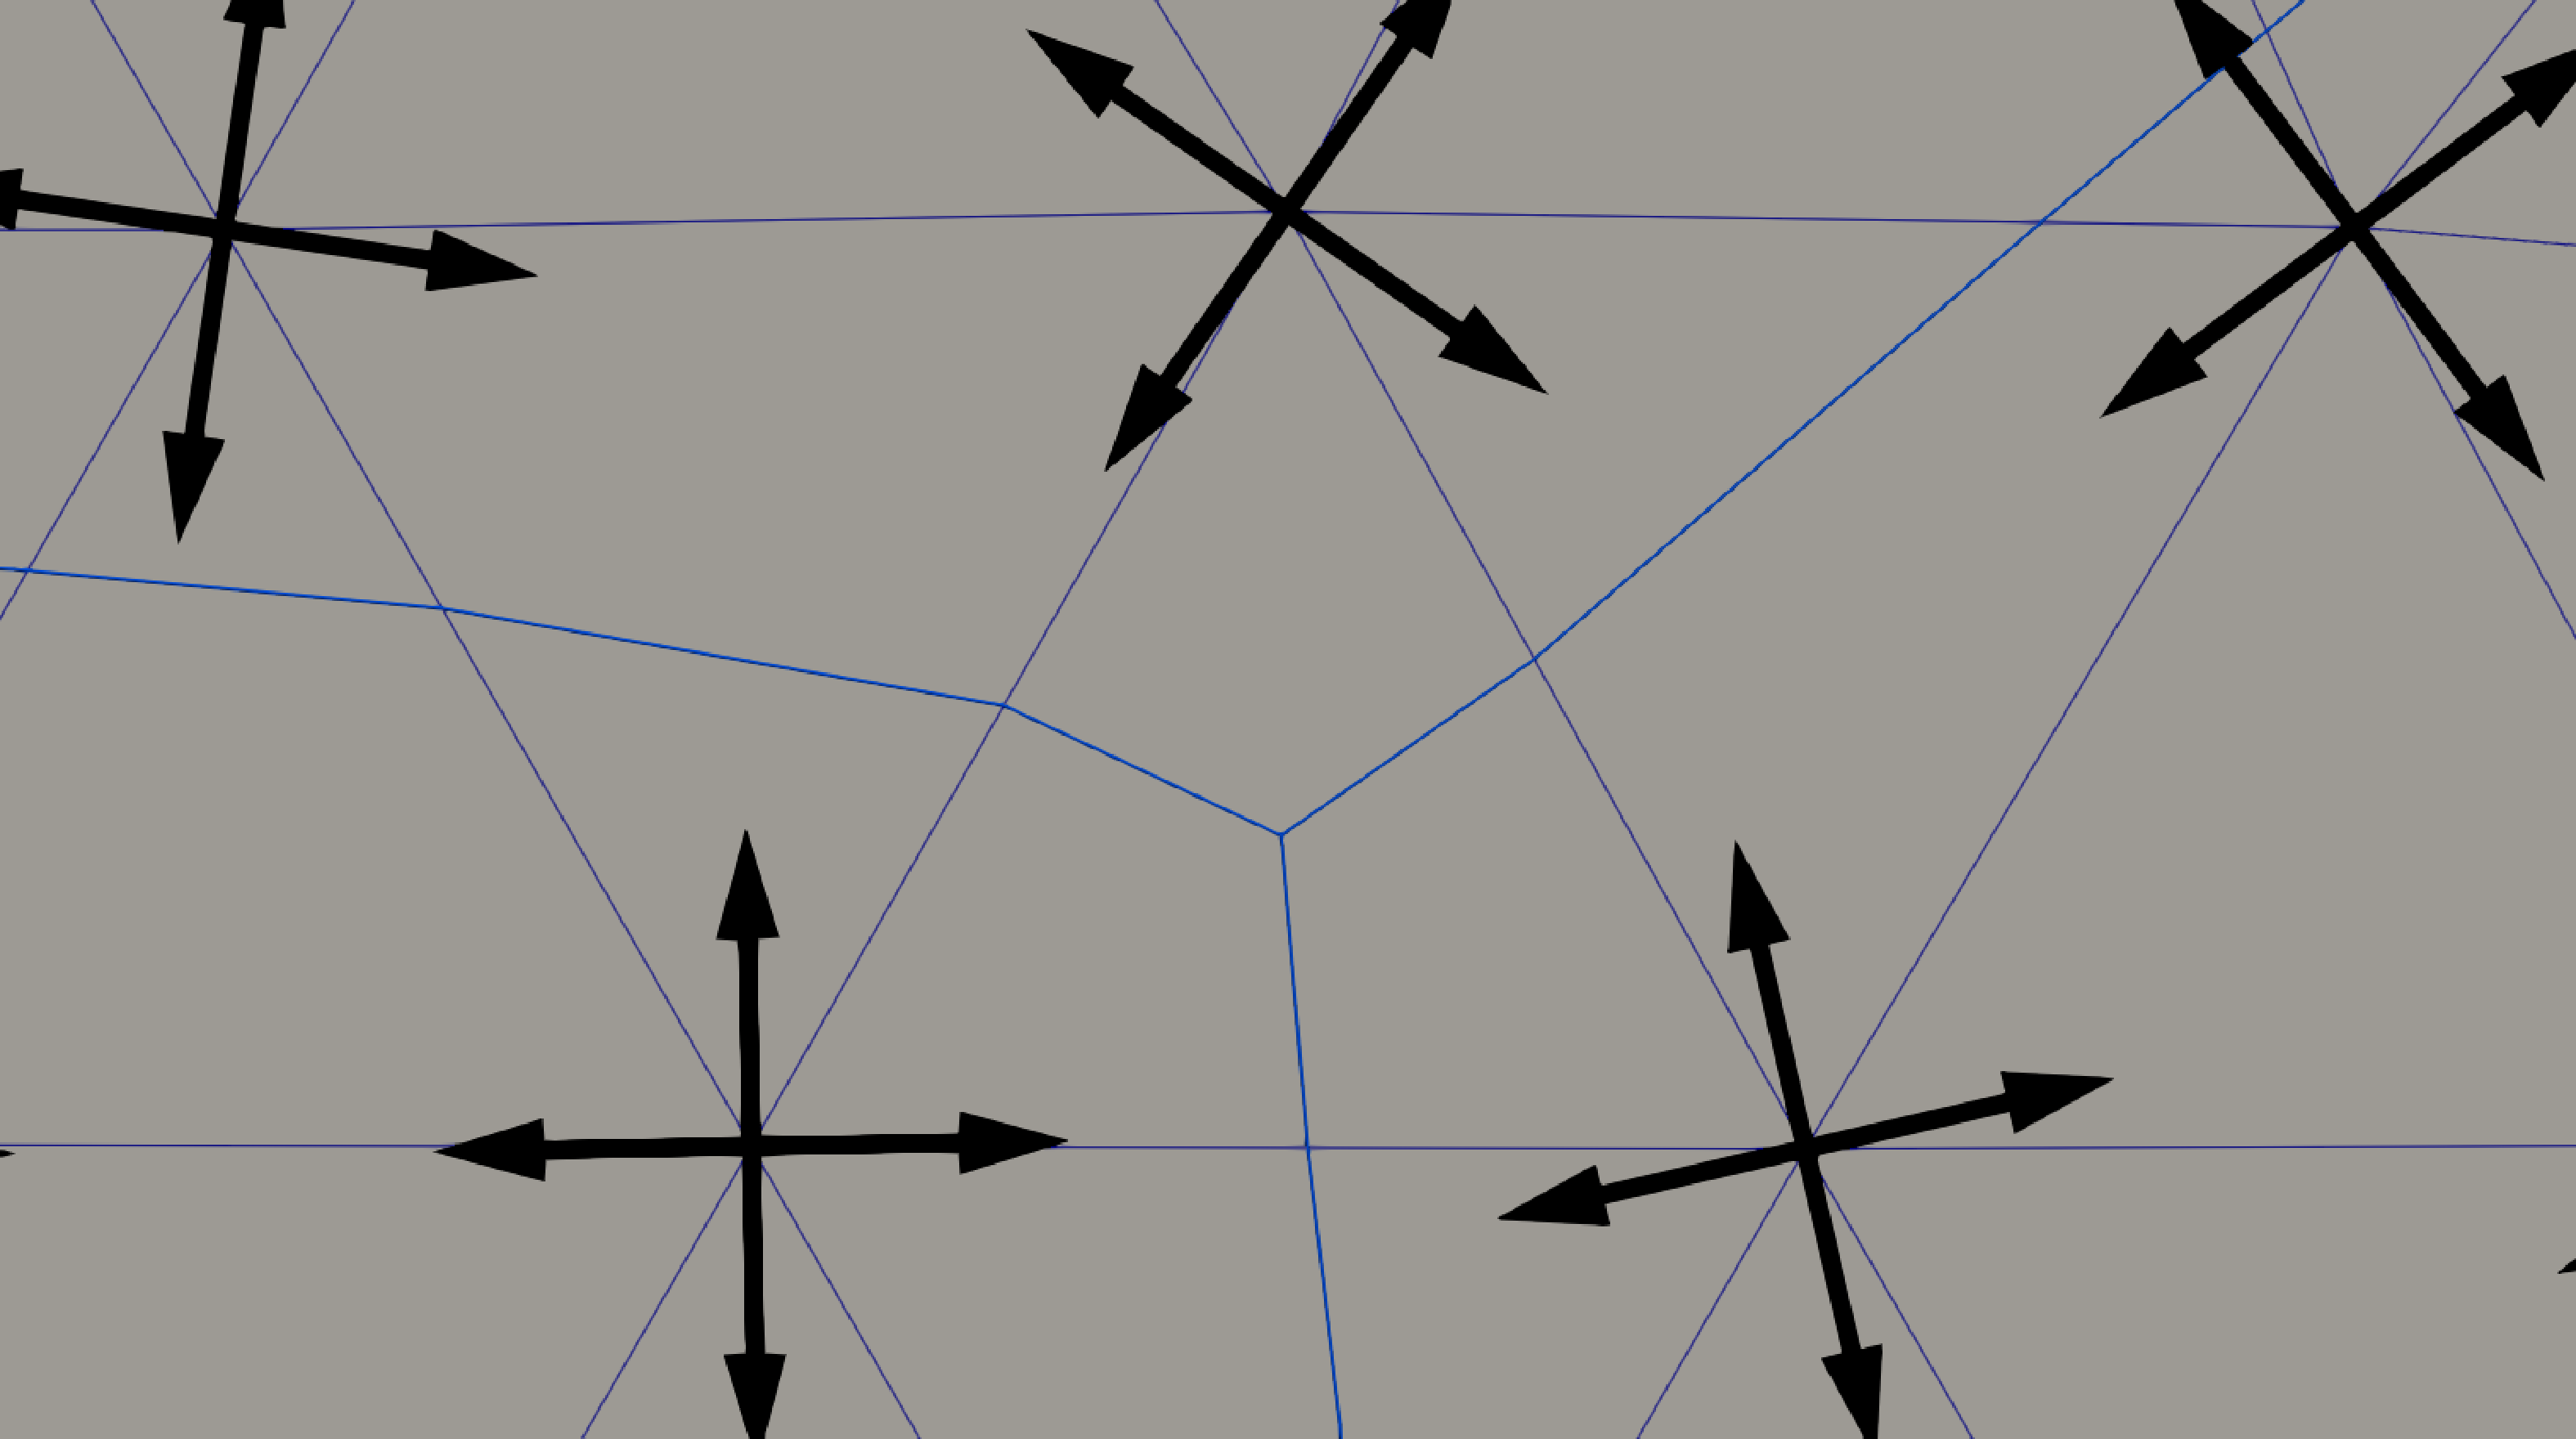
\includegraphics[width=\textwidth]{images/depart_sepa_1.pdf}
    \caption{Répartition uniforme des différences angulaires entre les directions de sortie.}
\end{subfigure}
\\[0.5cm]
\begin{subfigure}[b]{0.7\textwidth}
    \centering
    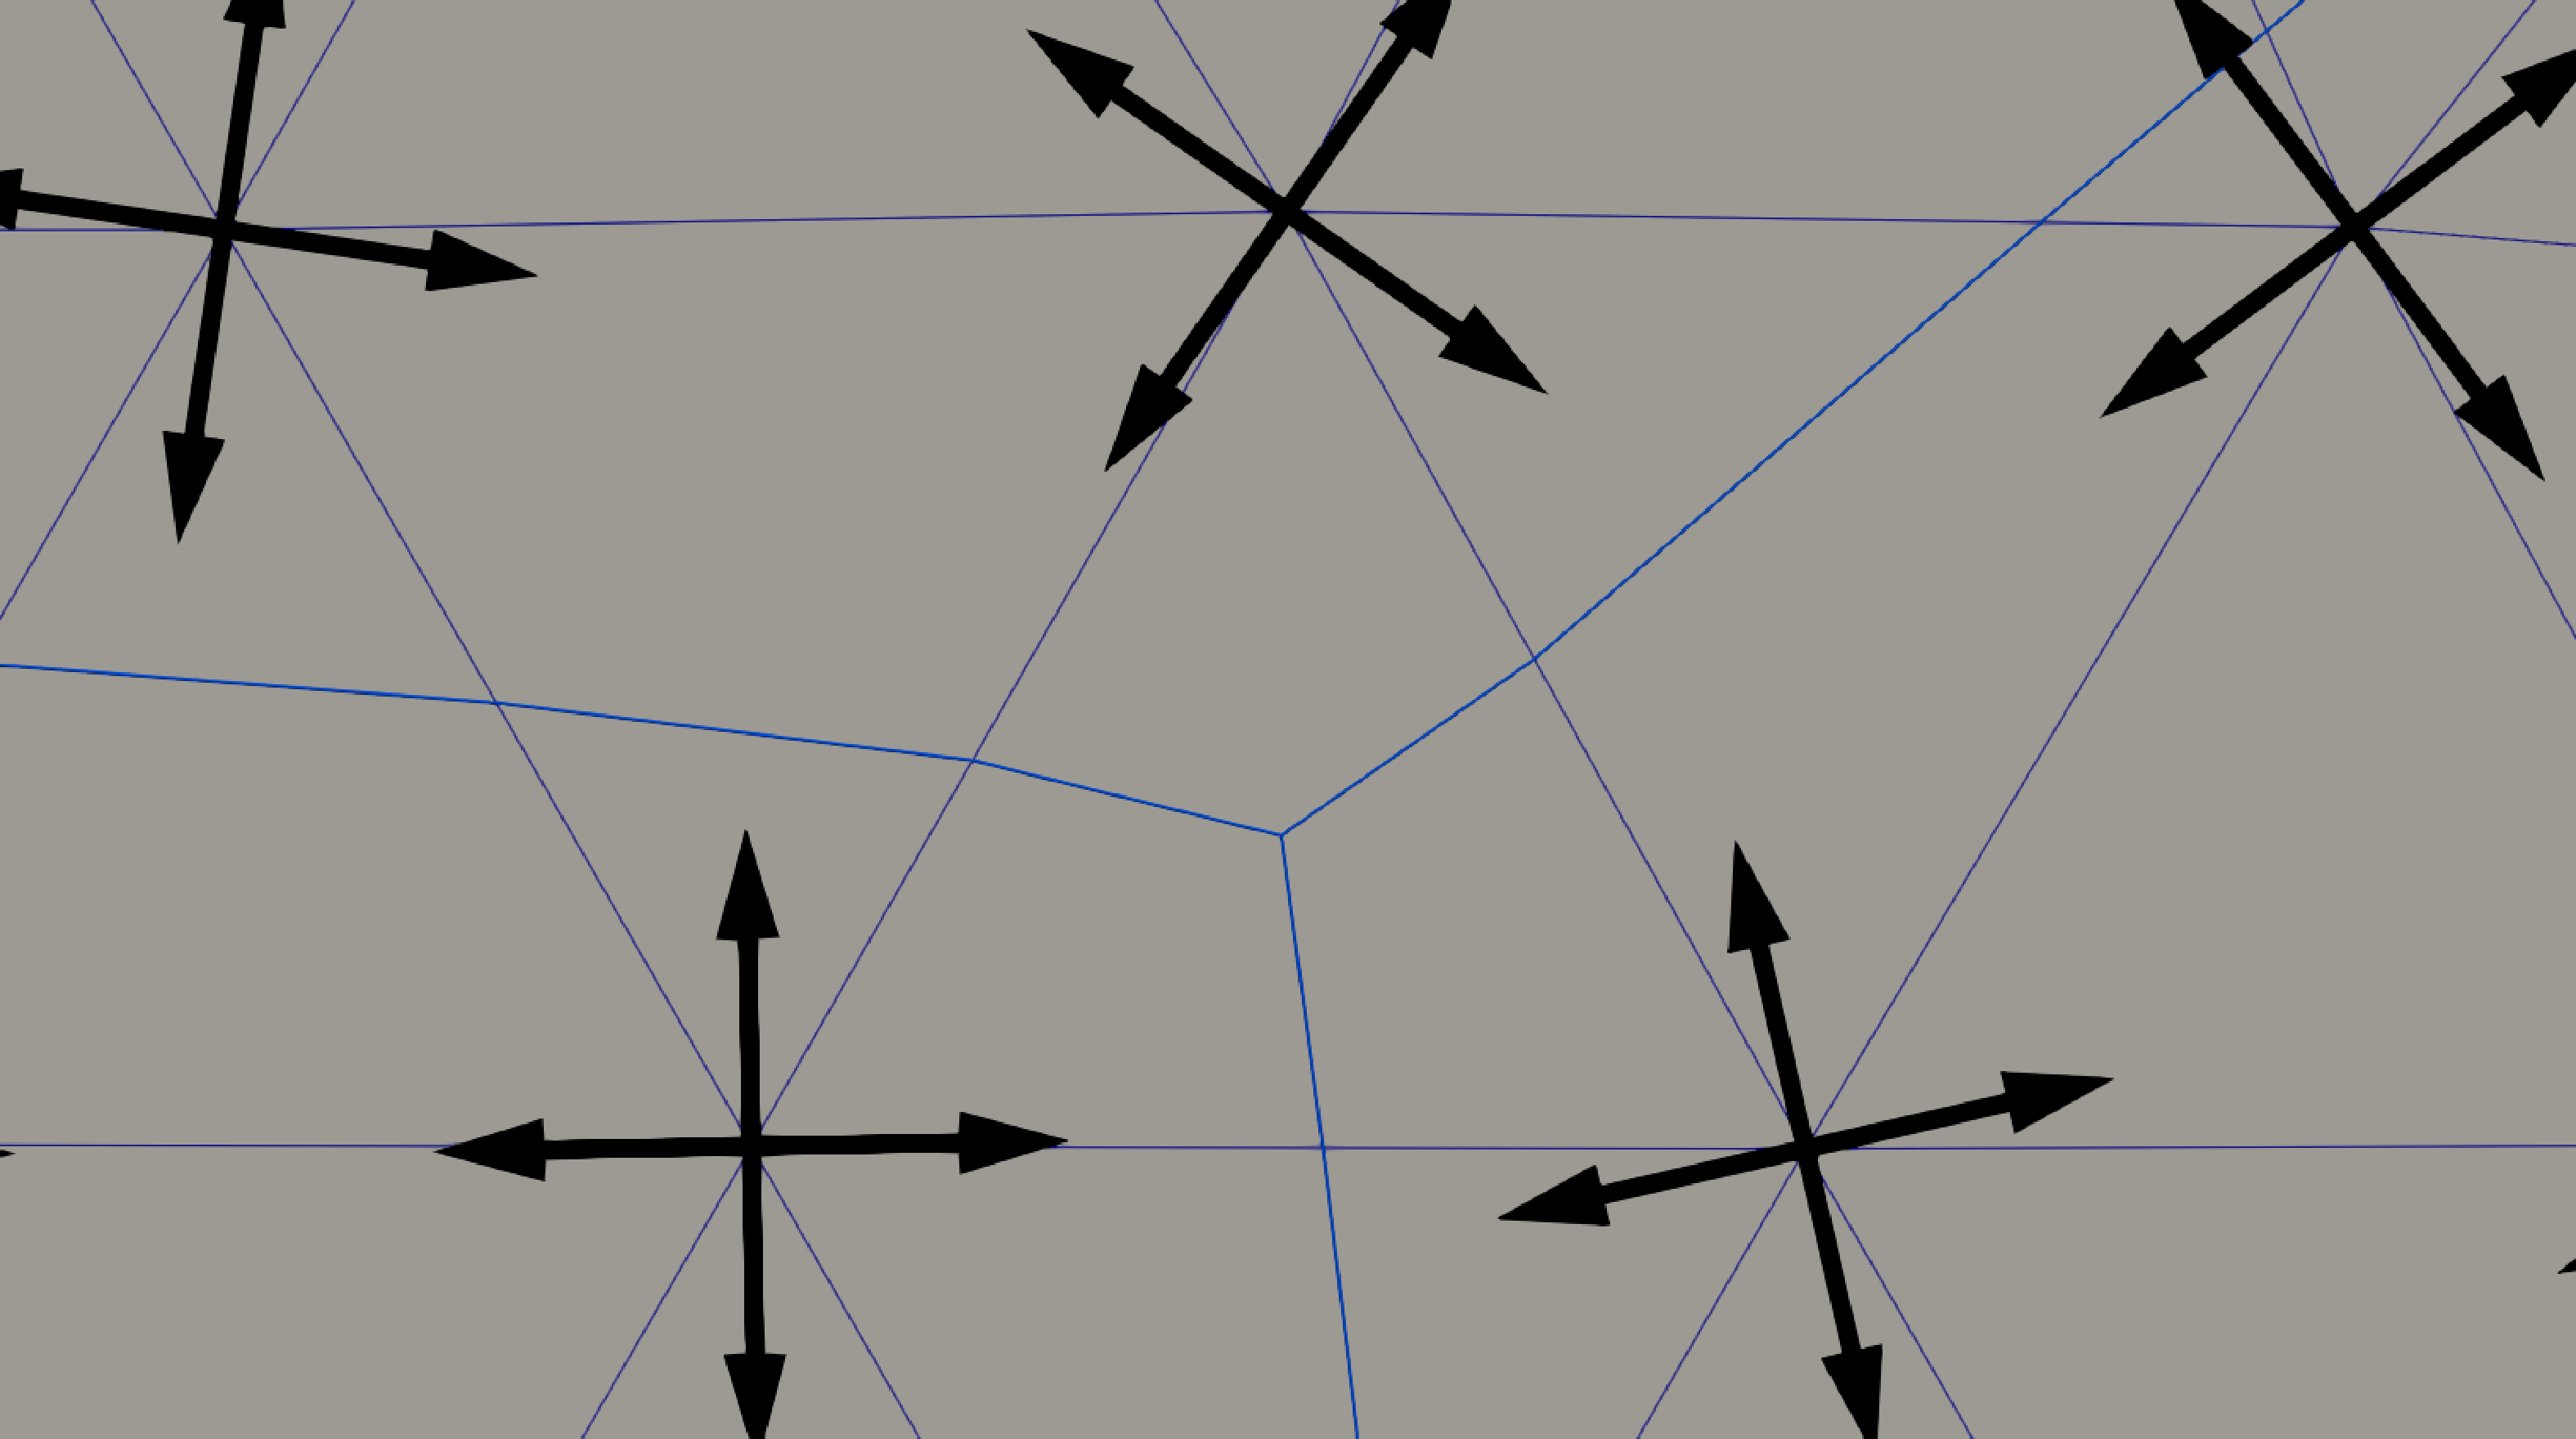
\includegraphics[width=\textwidth]{images/depart_sepa_2.pdf}
    \caption{Calcul des directions de sortie à l'aide de notre méthode.}
\end{subfigure}
\caption{Illustration des directions de sortie des séparatrices d'un point singulier d'indice $1/4$, utilisant deux méthodes distinctes.}
\label{fig:first_dir}
\end{figure}


Le principe demeure inchangé lorsque $p_0$ est un point singulier de bord ($p_0\in\mathcal{S}_{\bar{u}_h}\cap\partial\Omega_h$) (voir la figure \ref{fig:init_streams_bord}). Dans ce cas, le premier point $q_1$ est unique et correspond à $\gamma(0)$ où $\gamma$ est une paramétrisation sur $[0, 1]$ de $\partial Z{p_0}\backslash\partial\Omega_h$ dans le sens positif. Une fois les orientations initiales déterminées, l'intégration d'une séparatrice correspond exactement au processus d'intégration d'une ligne de champ tel que décrit dans la section \ref{subsec:pt_sing_ind_lign_champ}.

\begin{remark}
Dans la littérature, les directions initiales sont souvent calculées de manière uniforme autour du point singulier. Par exemple, pour un point singulier d'indice $1/4$, les directions initiales des trois séparatrices sont espacées d'une différence angulaire de $2\pi/3$ les unes des autres. Nous observons ainsi que la méthode d'initialisation que nous proposons ci-dessus est plus précise et fournit de meilleurs résultats (voir la figure \ref{fig:first_dir}).
\end{remark}


\paragraph{Intégration d'une séparatrice:}
Une fois la séparatrice initialiser, elle est intégré sur le mailllage en utilisant l'équation \eqref{eqn:stream_equation}. De façon général, nous construisons une approximation $SL^h_{\bar{u}_h}(p_0, \overrightarrow{u_0})$ de $SL_{\bar{u}_h}(p_0, \overrightarrow{u_0})$ sur $\Omega_h$ sous la forme d'une séquence de segments, élaborée en utilisant la méthode de Heun \cite{ascher1998computer} telle qu'exposée dans \cite{kowalski2013pde}. Le premier segment est représenté par $[p_0p_1]$ où $p_1$ est le point d'intersection entre $\partial T_{p_0}$ et la demi-droite d'origine $p_0$ et de vecteur directeur $\overrightarrow{u_0}$. Ensuite, pour tout $i\geq 1$, on construit le segment  $[p_ip_{i+1}]$ en cherchant le point $p_{i+1}$ comme le point d'intersection entre $\partial T_{p_i}$ et la demi-droite d'origine $p_i$ et dirigée par le vecteur:
\begin{equation}
\overrightarrow{u_i}=\mathbf{V}(\bar{u}_h(p_i), \overrightarrow{p_{i-1}p_i})+\mathbf{V}(\bar{u}_h(p'_{i+1}), \overrightarrow{p_{i-1}p_i}),
\end{equation}
où $p'_{i+1}$ est le point d'intersection entre $\partial T_{p_i}$ et la demi-droite d'origine $p_i$ et dirigé par le vecteur $\mathbf{V}(\bar{u}_h(p_i), \overrightarrow{p_{i-1}p_i})$ et pour tout $(\mathbf{c},d)\in\mathbf{C}\backslash\{0\}\times\mathbb{R}^2$, $\mathbf{V}(\mathbf{c}, d)$ désigne le vecteur $\mathbf{c}$ qui s'aligne le mieux avec la direction $d$. Autrement dit, il s'agit de l'unique élément de l'ensemble:
\begin{equation}
\{\mathbf{V}(\mathbf{c}, d)\}=\underset{c_k\in\mathbf{c},~k\in\llbracket1, 4\rrbracket}{\mathrm{argmin}}|c_k.d\|d\|^{-1}-1|.
\end{equation}
Une illustration de ce processus est donné sur la figure \ref{fig:draw_streams_1}.

\begin{figure}[!h]
     \centering
     \begin{subfigure}[b]{0.7\textwidth}
         \centering
         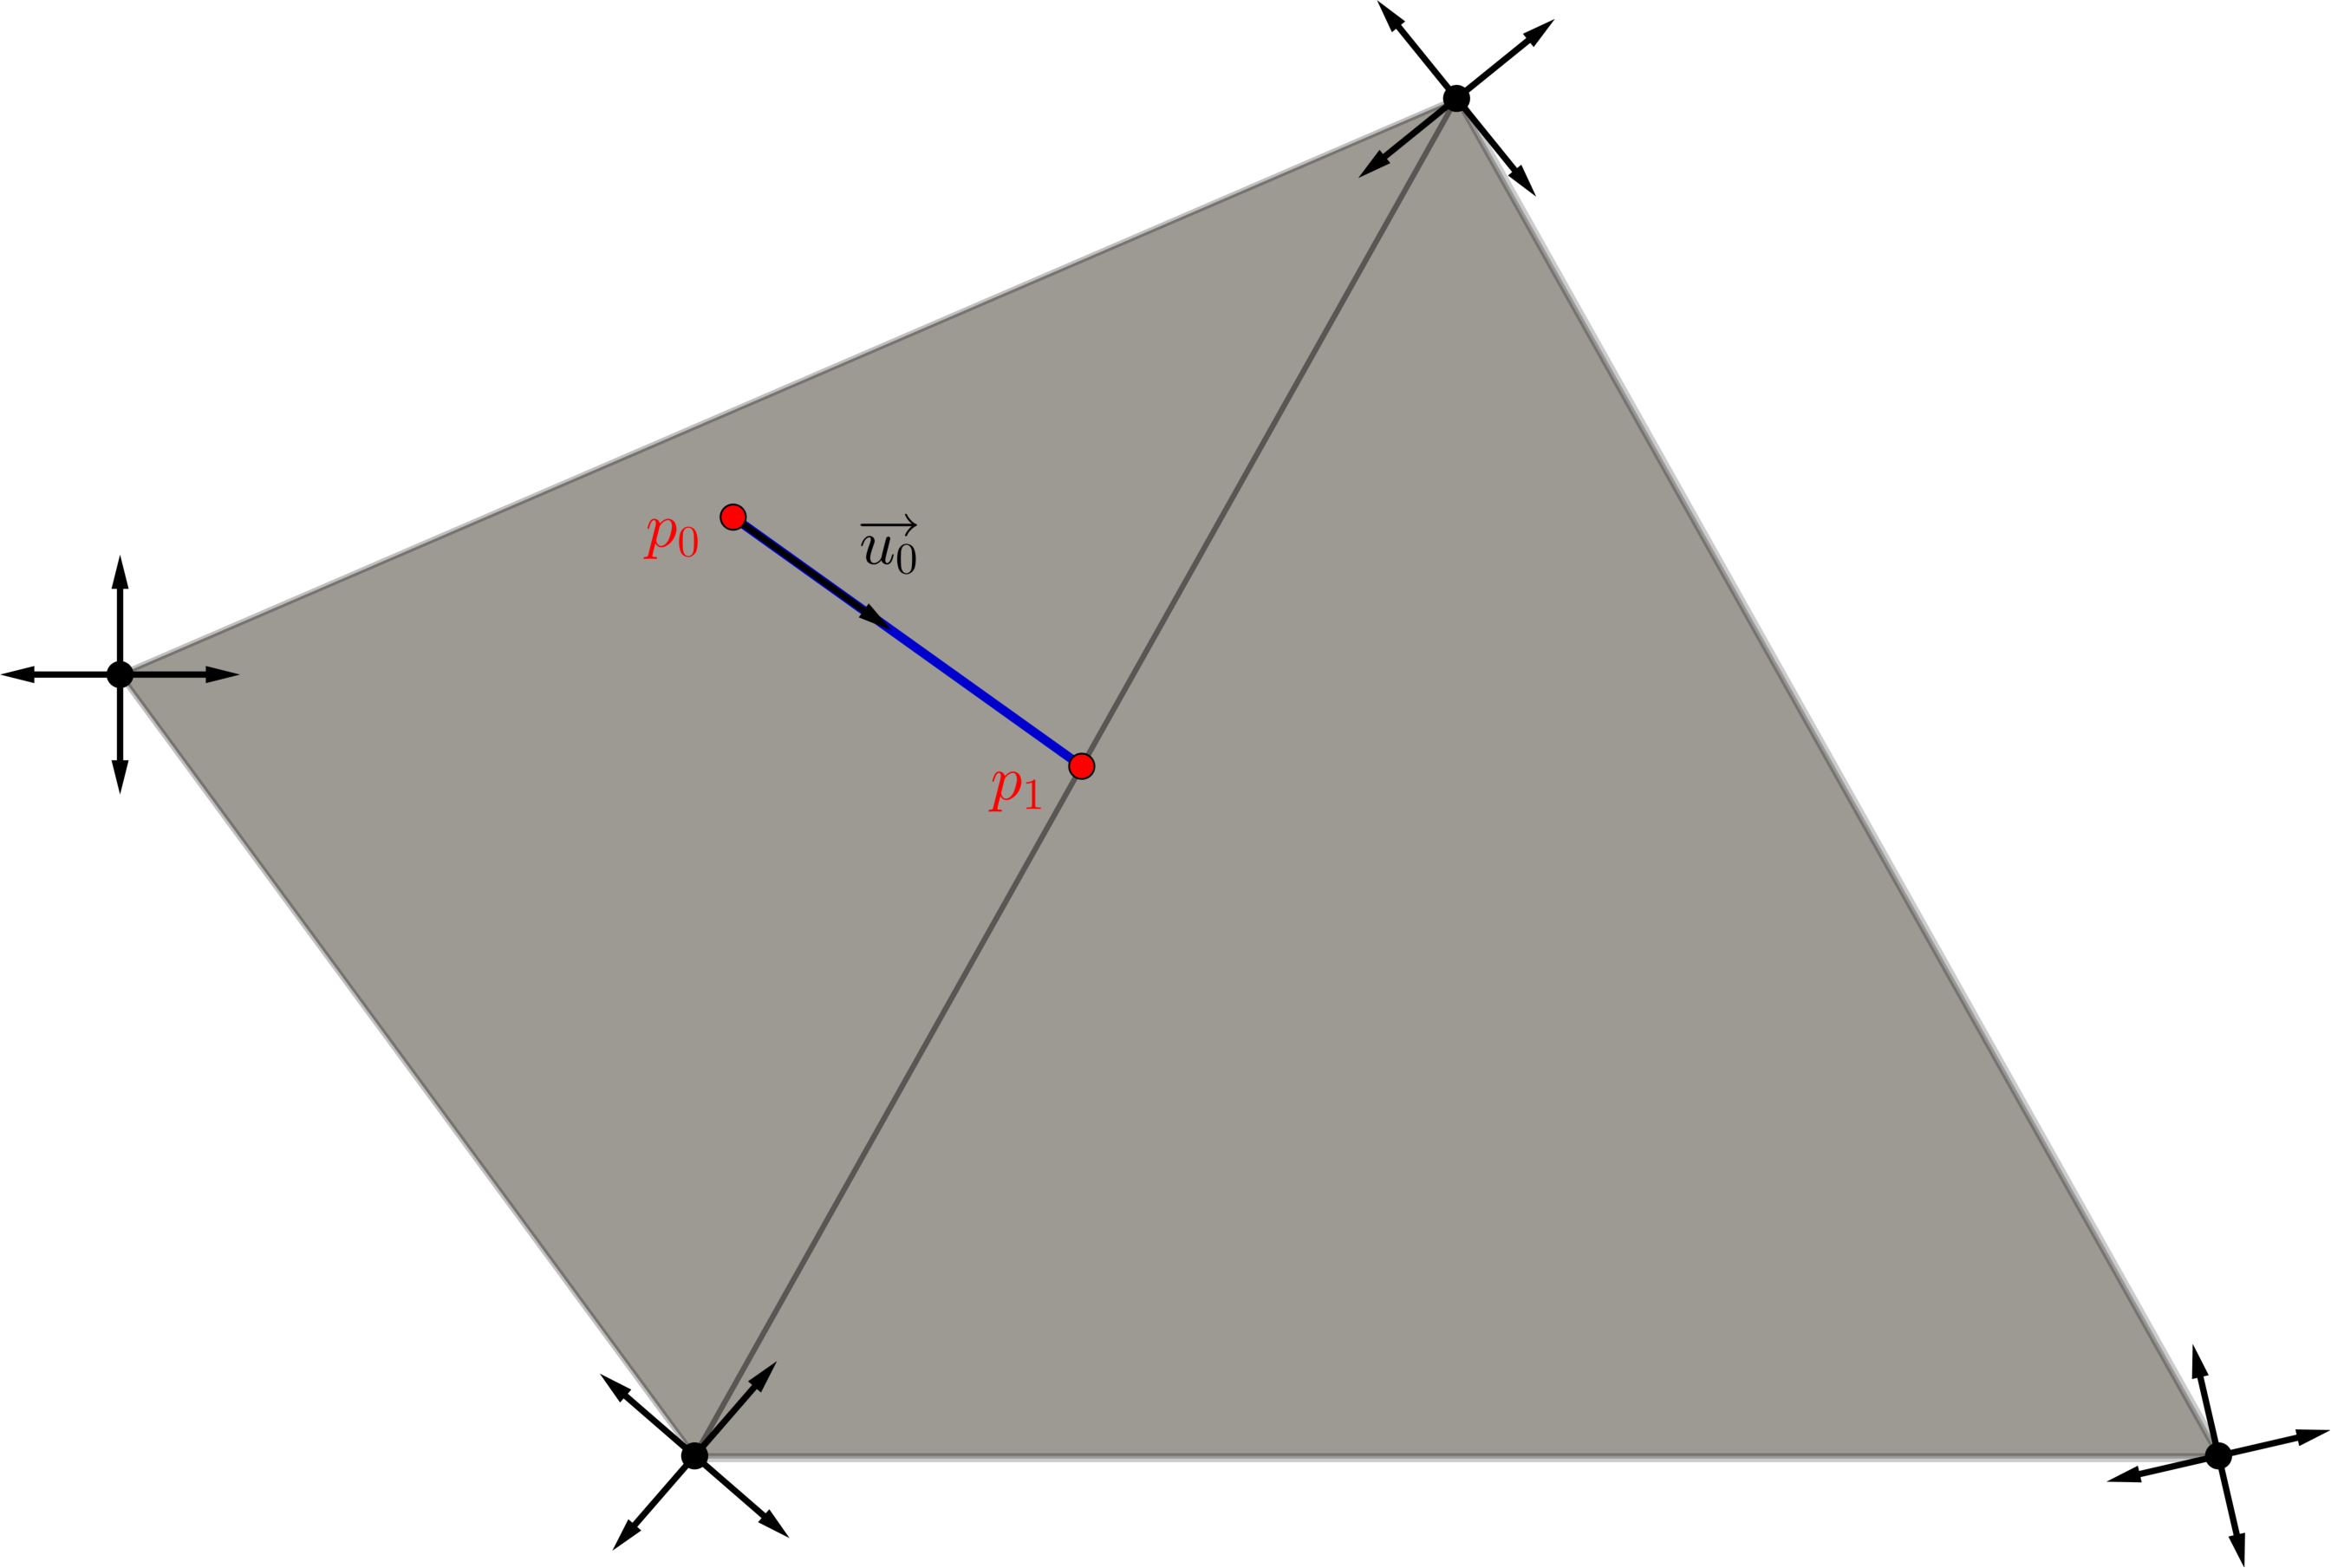
\includegraphics[width=\textwidth]{images/draw_streams_11.pdf}
         \caption{Construction du premier segment de la ligne de champ.}
     \end{subfigure}
     \begin{subfigure}[b]{0.7\textwidth}
         \centering
         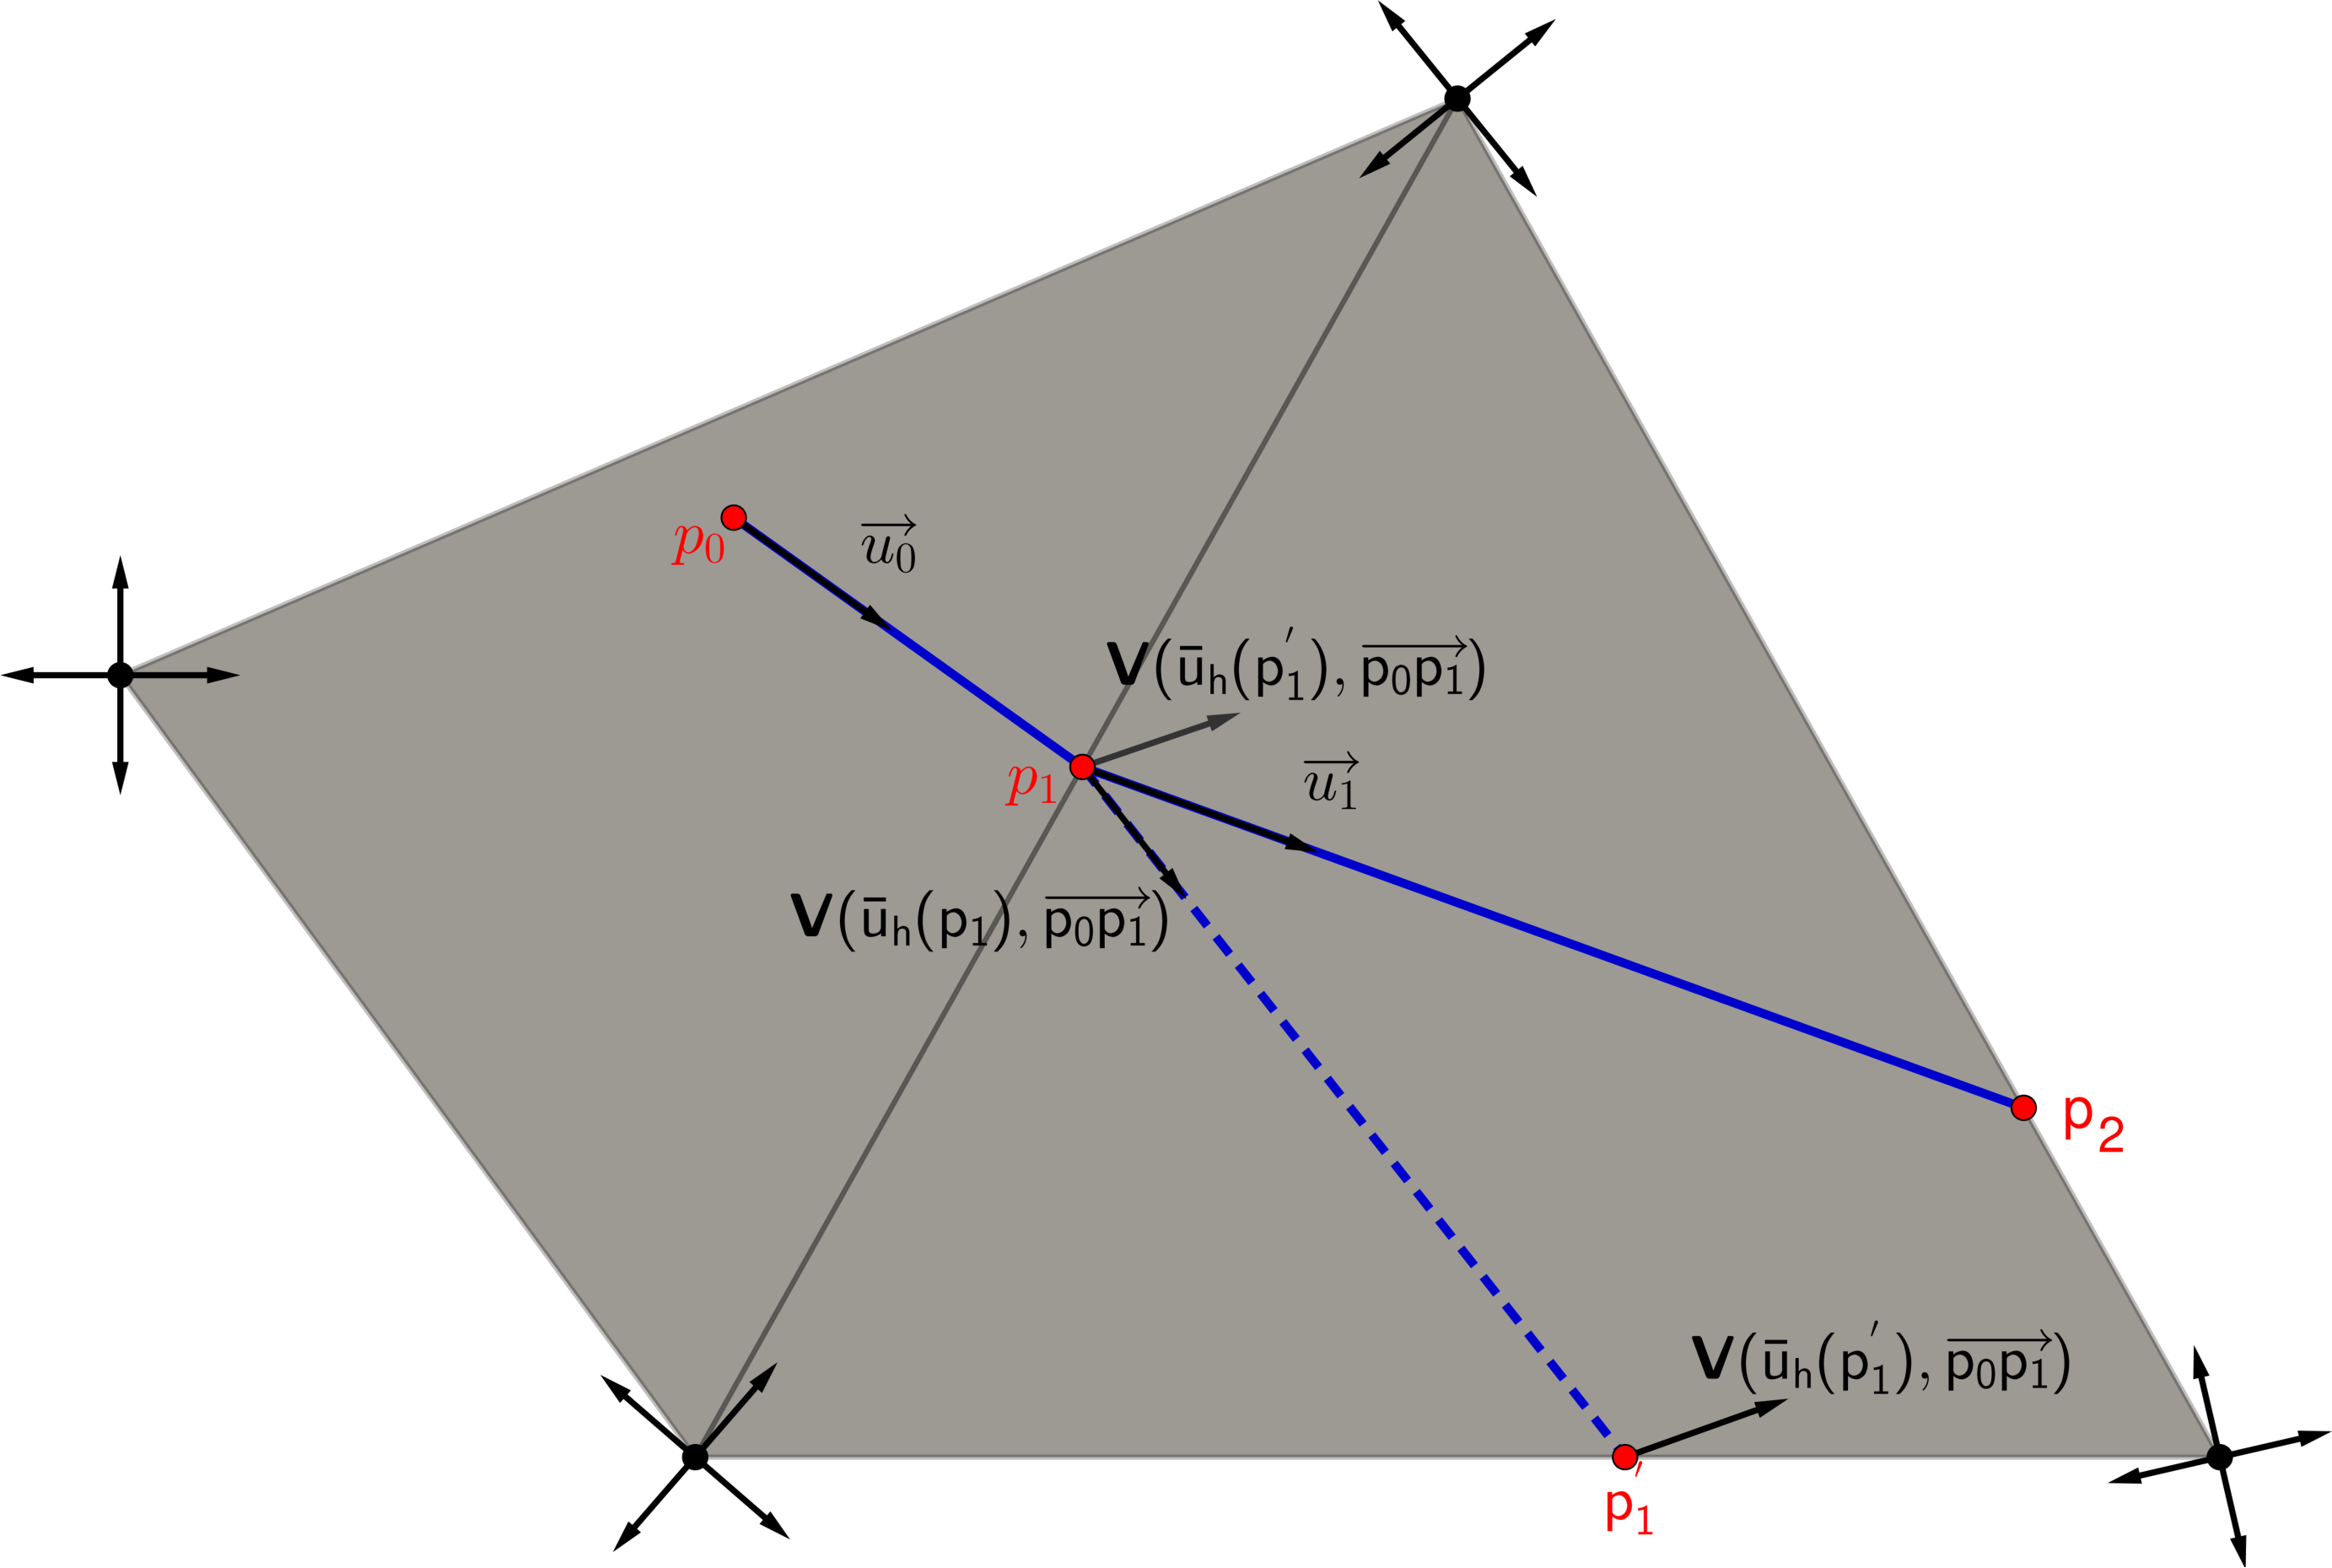
\includegraphics[width=\textwidth]{images/draw_streams_12.pdf}
         \caption{Intégration de la ligne de champ dans un triangle.}
     \end{subfigure}
        \caption{Approximation d'une ligne de champ par la méthode de Heun.}
        \label{fig:draw_streams_1}
\end{figure}

Une approche alternative, plus efficace et rapide pour construire les segments $[p_ip_{i+1}]$ pour $i\geq 1$, consiste à exploiter la proposition \ref{prop:align_sepa_voisinnage}. Considérons $L_T=SL_{\bar{u}_h}\cap T$, la portion de la ligne de champ $SL_{\bar{u}_h}$ se trouvant dans un triangle $T$ et que l'on souhaite représenter par un segment $[p_ip_{i+1}]$. Ici, $p_i$ et $p_{i+1}$ représentent les points d'intersection entre $L$ et le bord de $T$ (c'est-à-dire, $\{p_i, p_{i+1}\}=L\cap\partial T$) et le but est de trouver le point $p_{i+1}$. Or en modifiant le champ $\bar{u}_h$ dans le triangle d'après la proposition \ref{prop:align_sepa_voisinnage} on sait que l'on a $p\in T$ tel que:
\begin{equation}
W^\gamma_{\bar{u}_h}(p_{i+1})-W^\gamma_{\bar{u}_h}(p_i)=-\pi,
\label{eqn:formule_W}
\end{equation}
où $\gamma$ est une paramétrisation sur $[0, 1]$ de $\partial T$ dans le sens positif et pour tout $t\in[0, 1]$ on a $W^\gamma_{\bar{u}_h}(t)=\theta_{\bar{u}_h}^\gamma(t)-\arg{\overrightarrow{p\gamma(t)}}$. Il suffit donc de trouver une approximation du point $p$ puis d'exploiter l'équation \ref{eqn:formule_W} pour trouver une approximation de $p_{i+1}$. Dans notre cas, nous choisissons comme approximation du point $p$, le point $p_i^{'}$ vérifiant:
$$
p_i^{'}\in T\mbox{ et }\overrightarrow{p_ip_i^{'}}=\epsilon\overrightarrow{p_{i-1}p_i}, \mbox{ avec }\epsilon\in]0, 1[ \mbox{ très petit}.
$$
On trouve ensuite $p_{i+1}$ en utilisant l'équation \ref{eqn:formule_W} avec $W^\gamma_{\bar{u}_h}(t)=\theta_{\bar{u}_h}^\gamma(t)-\arg{\overrightarrow{p_i^{'}\gamma(t)}}$ (voir la figure \ref{fig:draw_streams_2}). C'est cette dernière approche que nous avons adopté dans notre implémentation.

\begin{figure}[!h]
     \centering
     \begin{subfigure}[b]{0.7\textwidth}
         \centering
         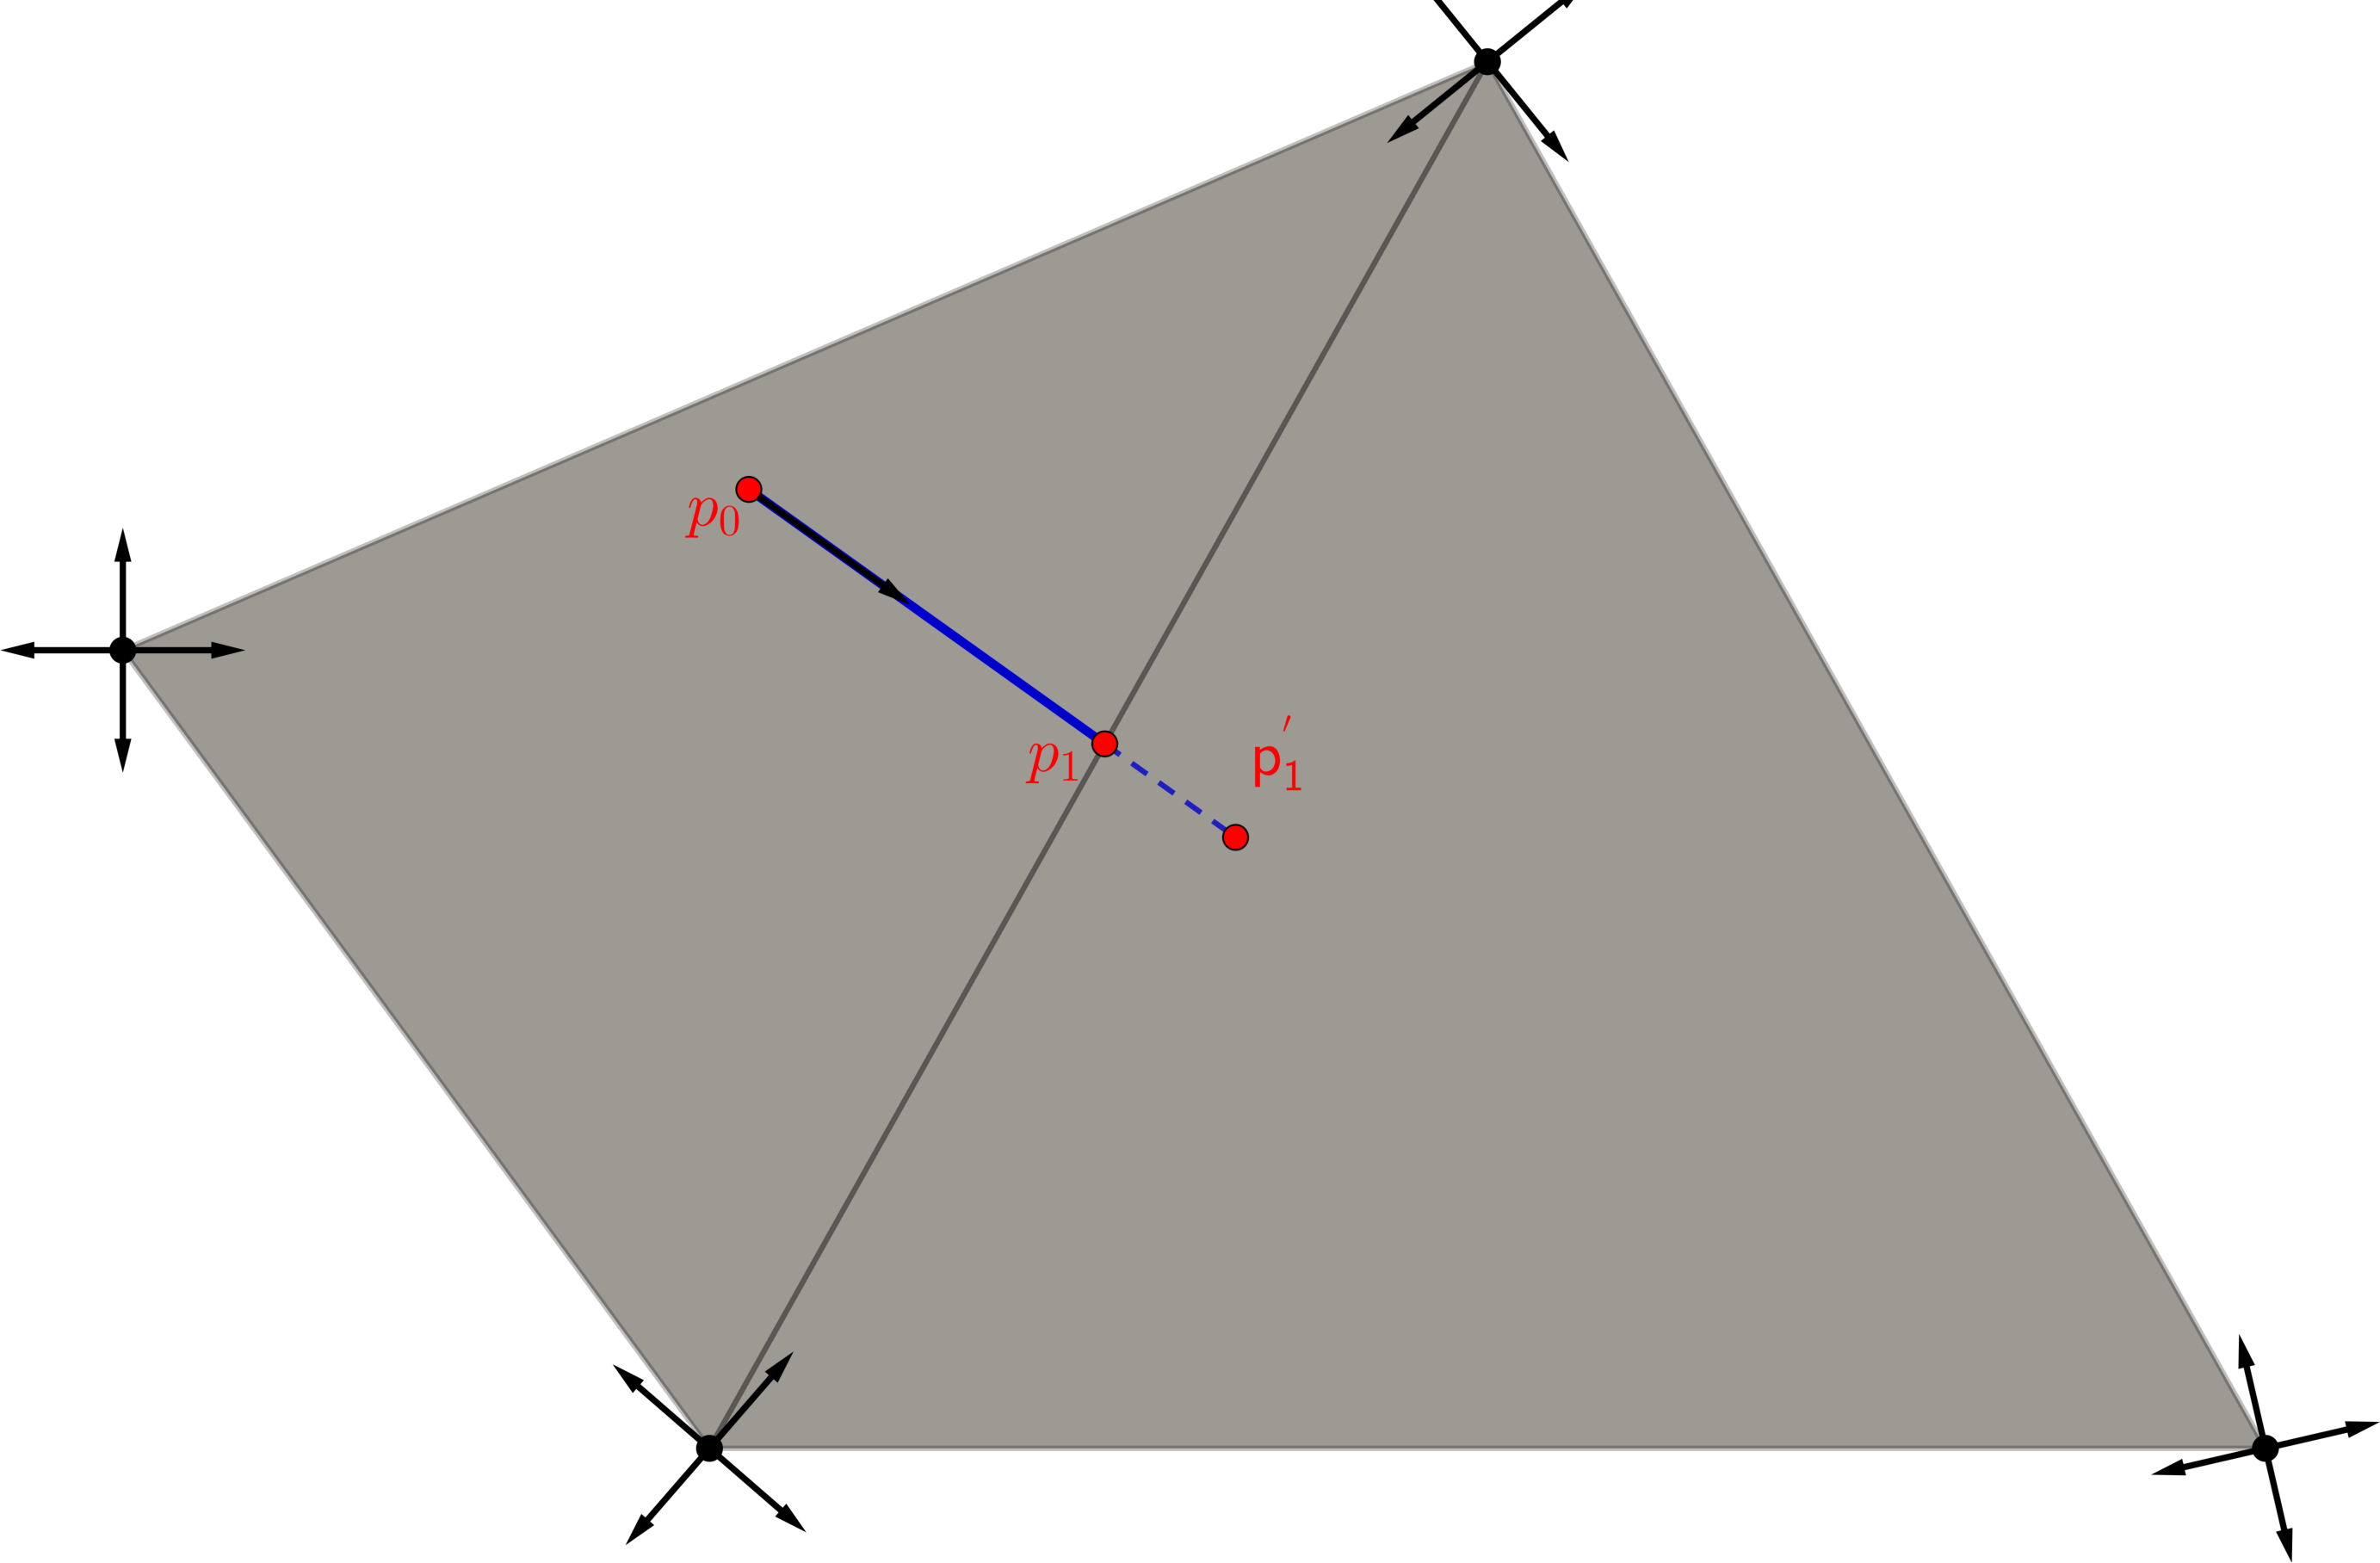
\includegraphics[width=\textwidth]{images/draw_streams_21.pdf}
         \caption{Construction du premier segment de la ligne de champ.}
     \end{subfigure}
     \begin{subfigure}[b]{0.7\textwidth}
         \centering
         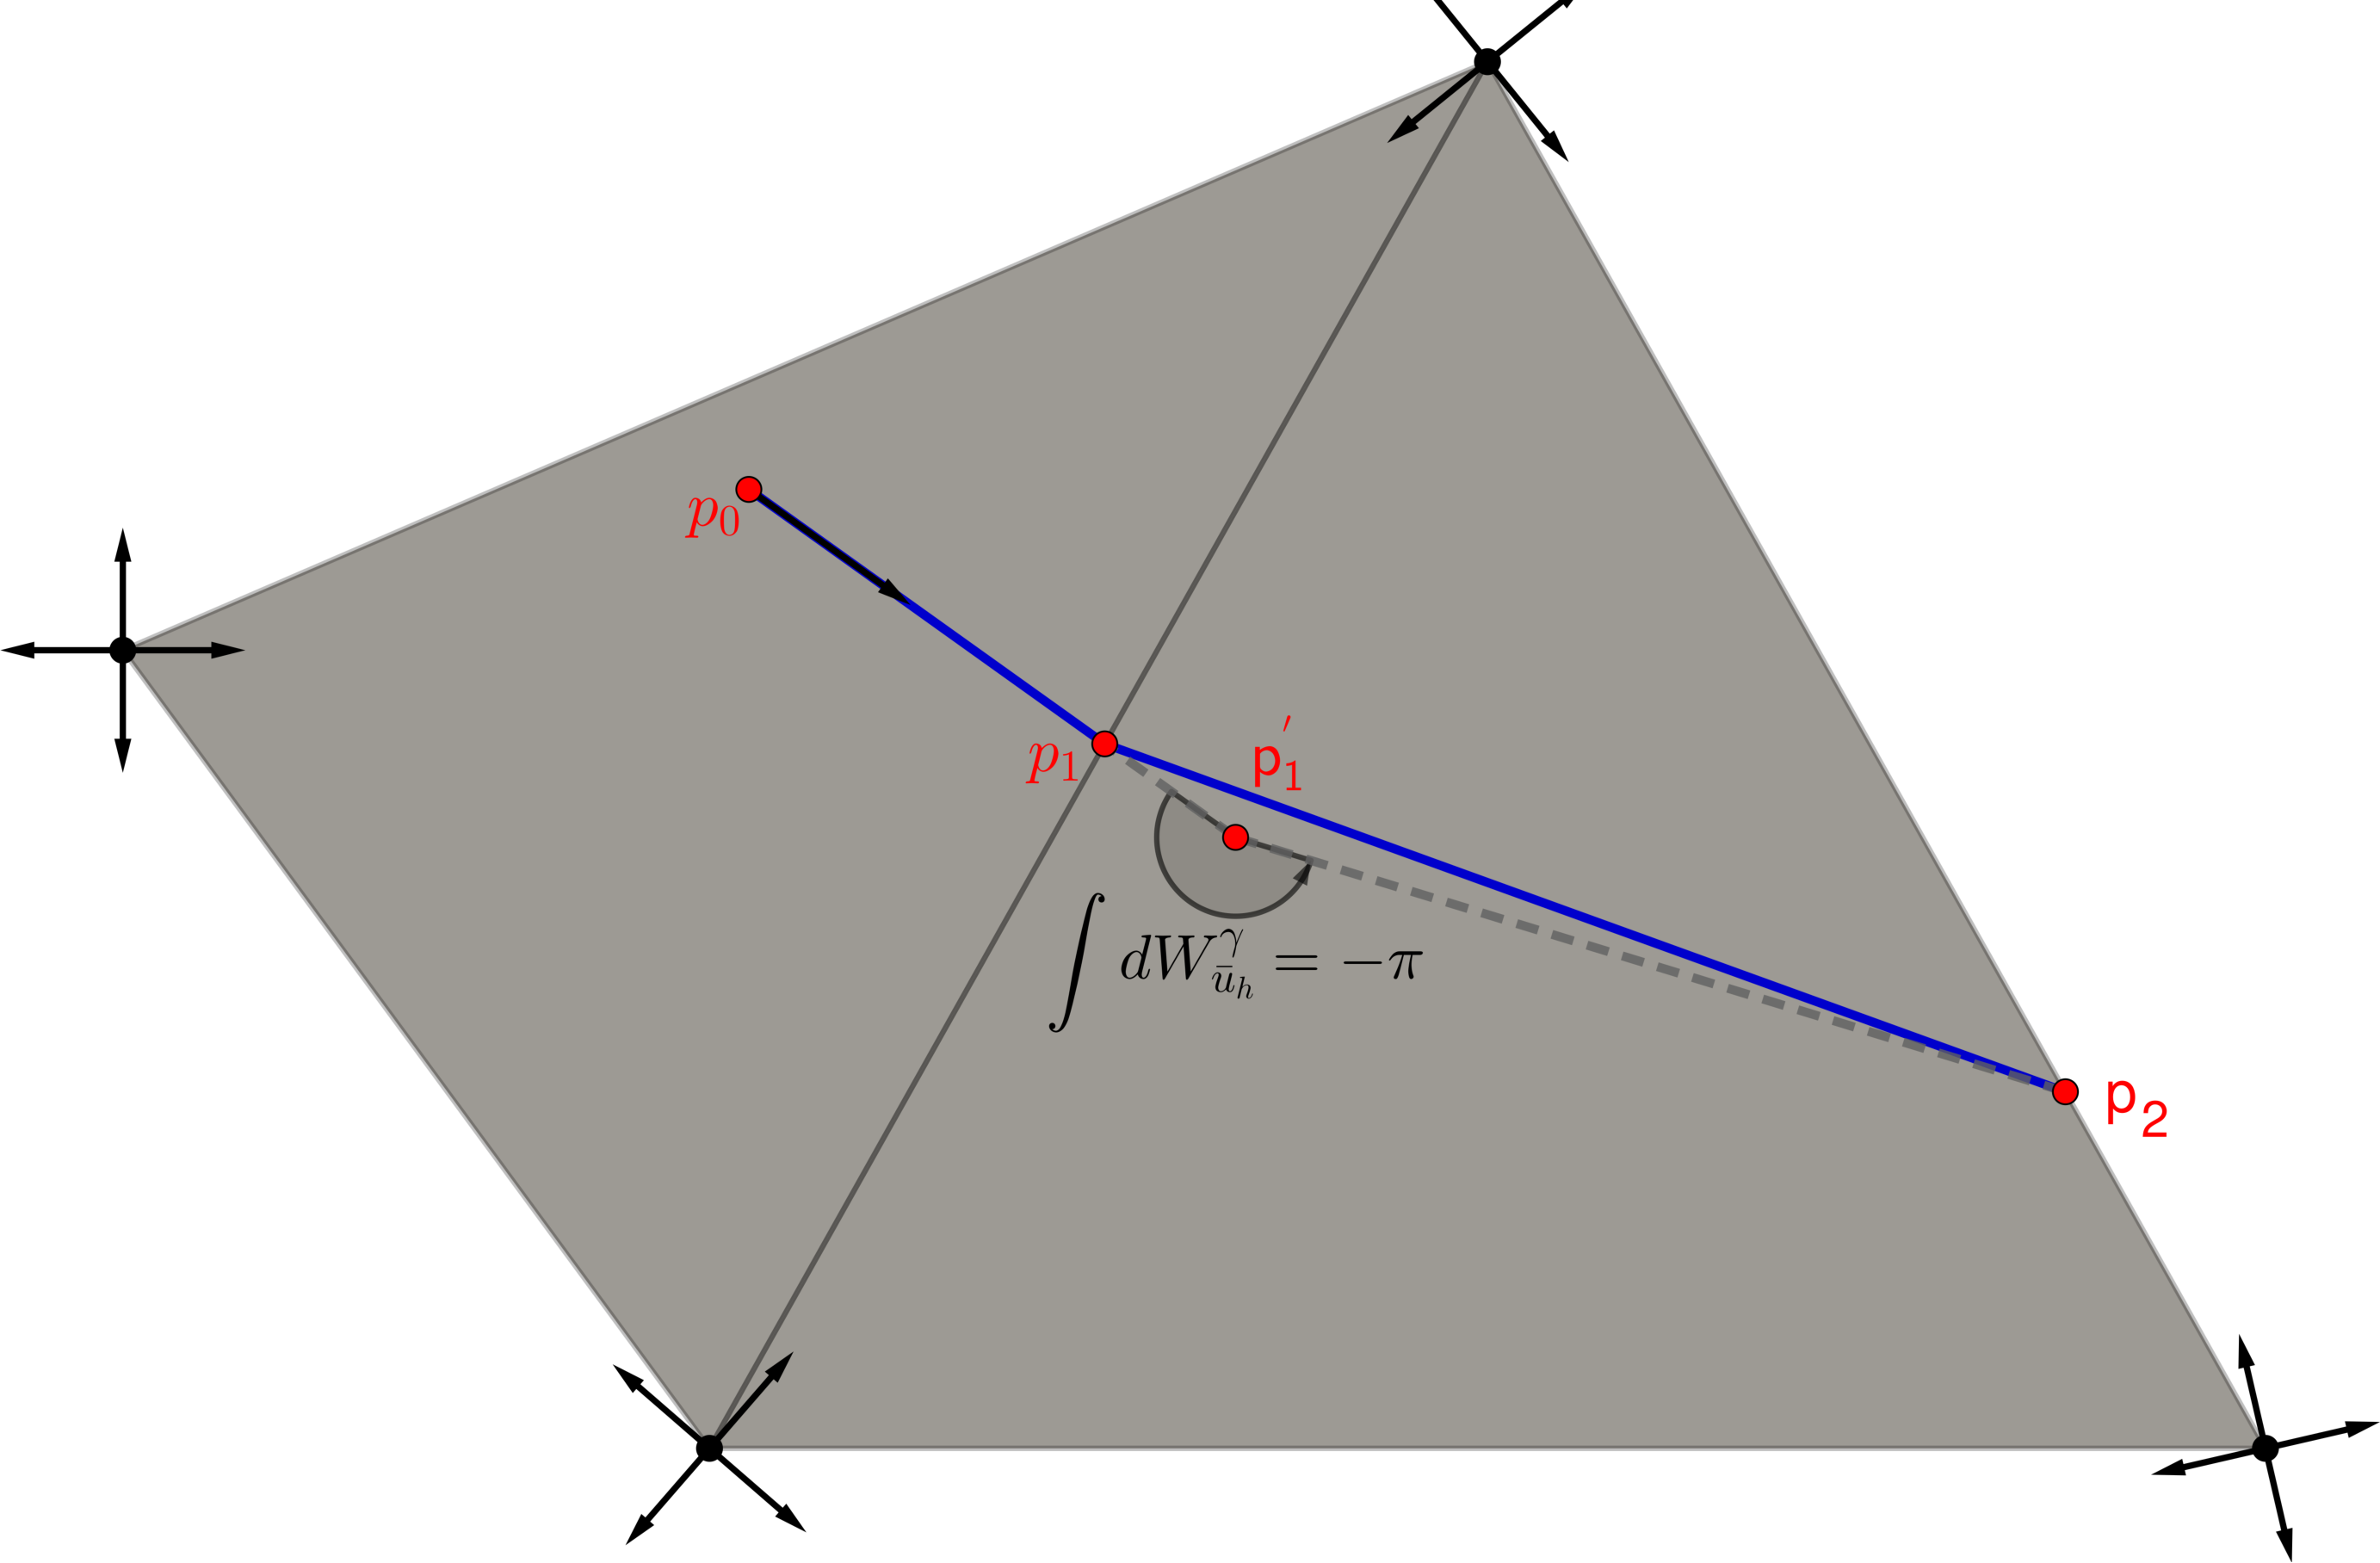
\includegraphics[width=\textwidth]{images/draw_streams_22.pdf}
         \caption{Intégration de la ligne de champ dans un triangle.}
     \end{subfigure}
        \caption{Approche alternative pour l'intéfration des lignes de champ dans un champ de croix.}
        \label{fig:draw_streams_2}
\end{figure}

\paragraph{Traversé d'un triangle singulier:}

\begin{figure}[!h]
\centering
\begin{subfigure}[b]{0.495\textwidth}
    \centering
    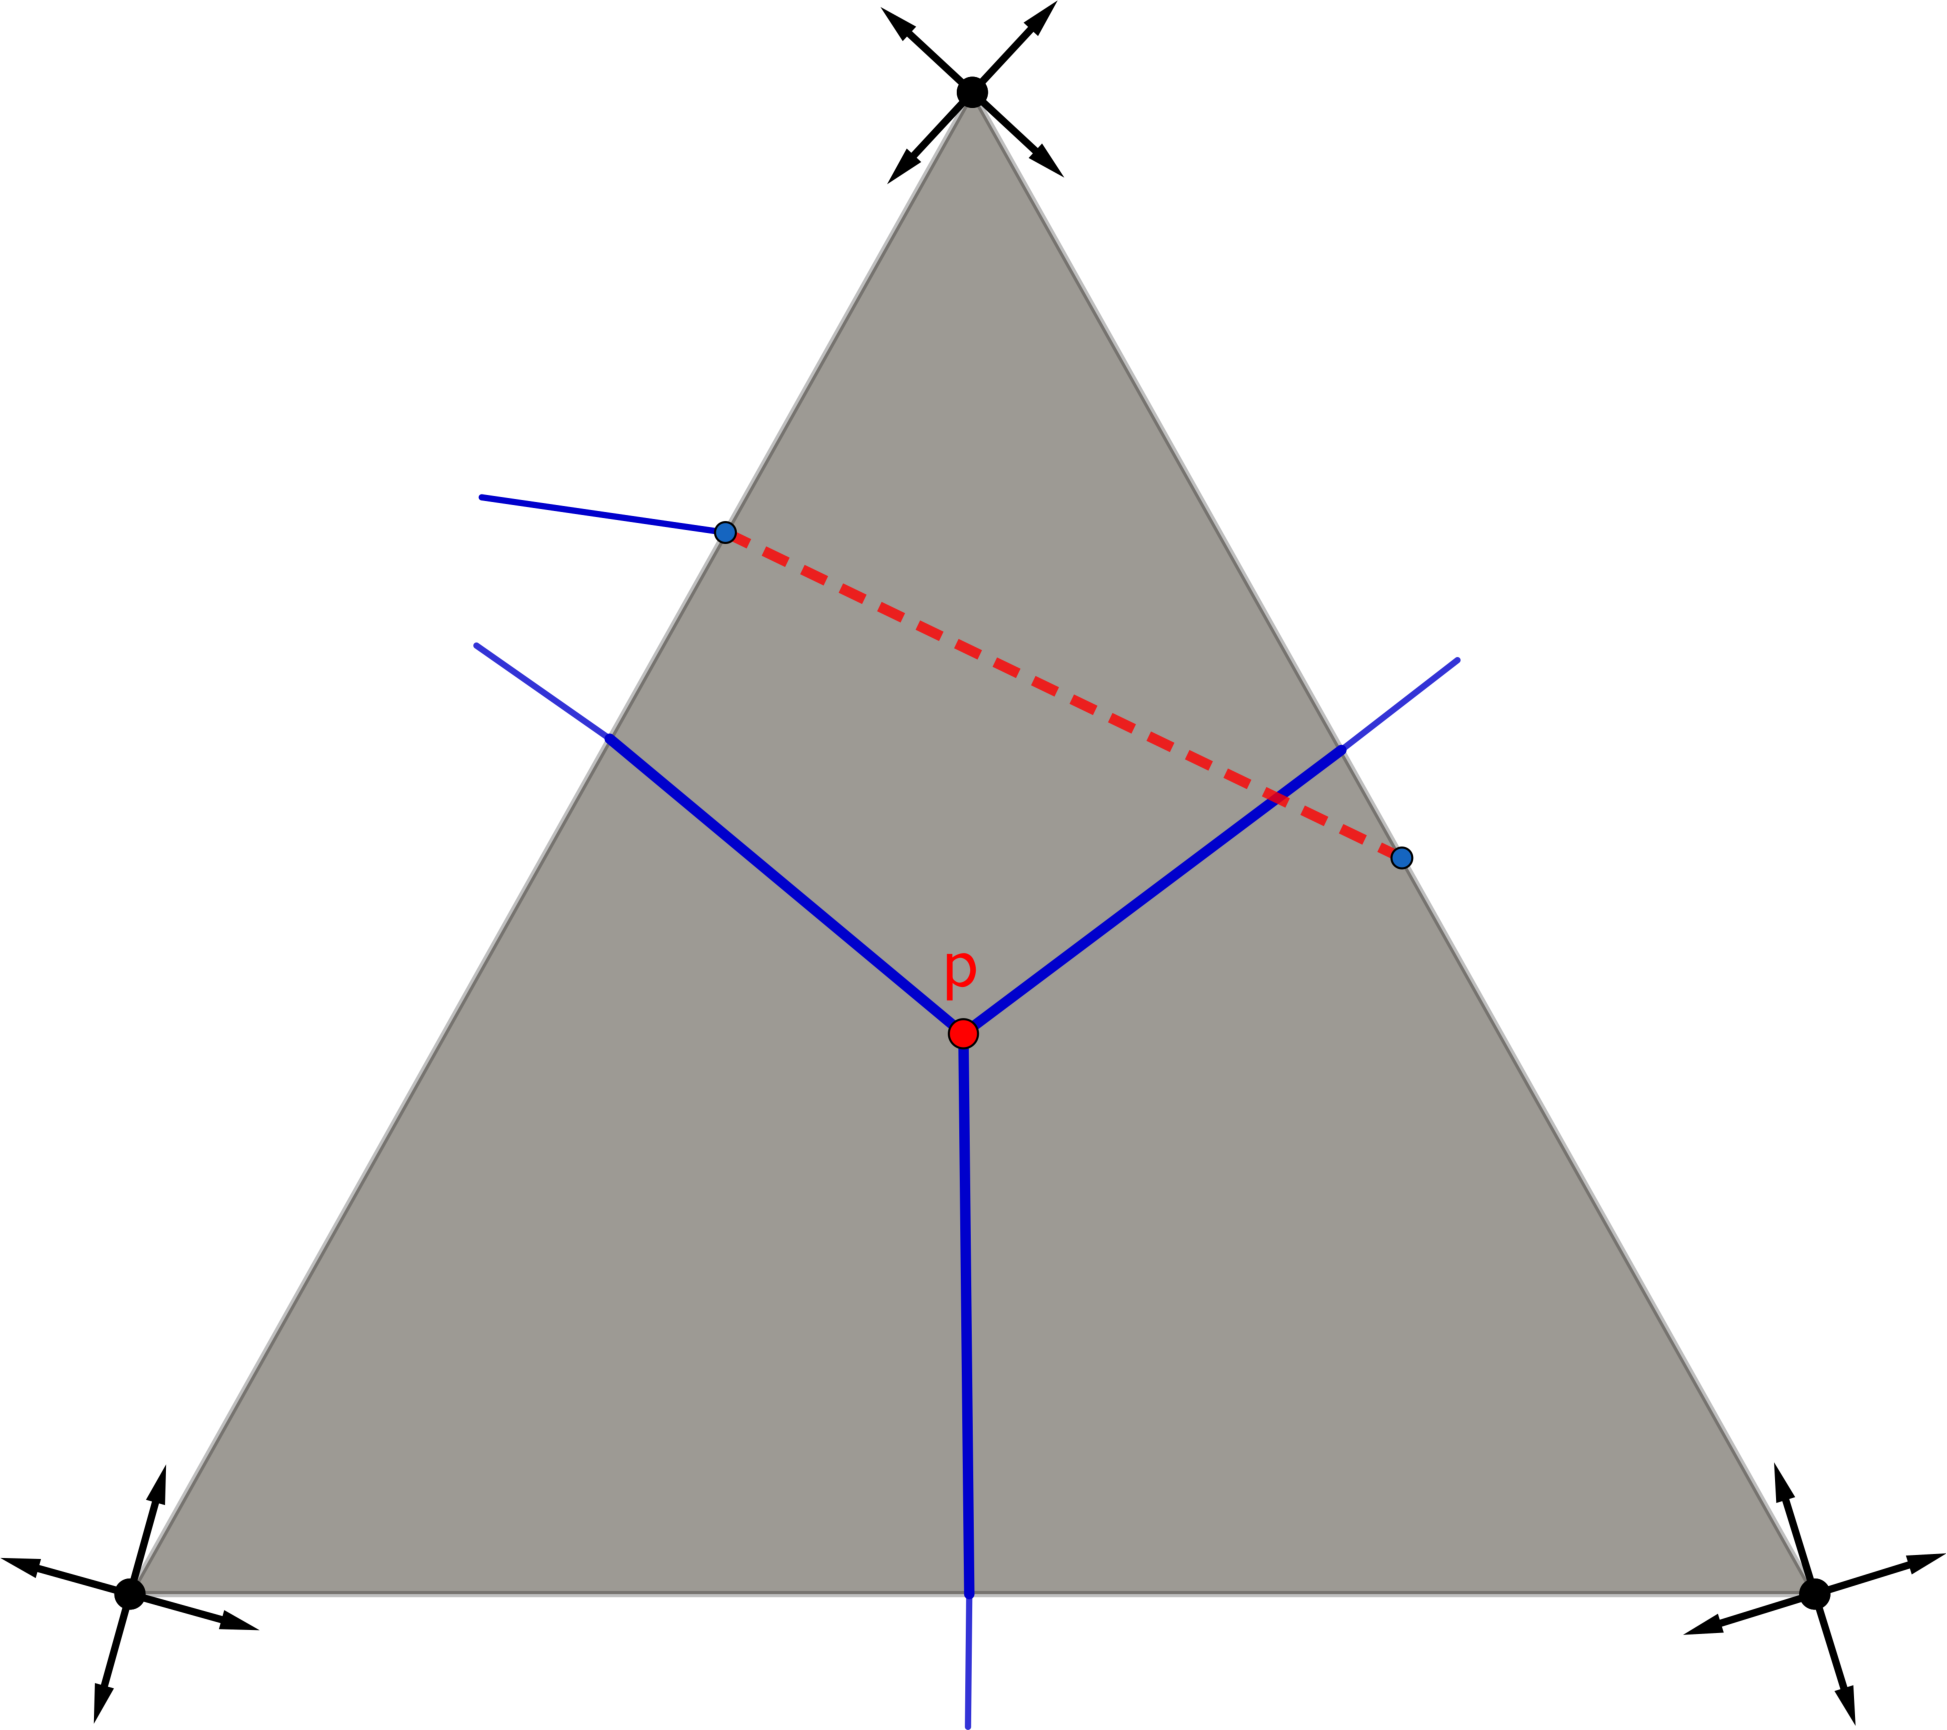
\includegraphics[width=\textwidth]{images/draw_streams_sing_1.pdf}
    \caption{\'Echec d'intégration d'une séparatrice dans un triangle singulier.}
    \label{fig:draw_streams_sing_1}
\end{subfigure}
\hfill
\begin{subfigure}[b]{0.495\textwidth}
    \centering
    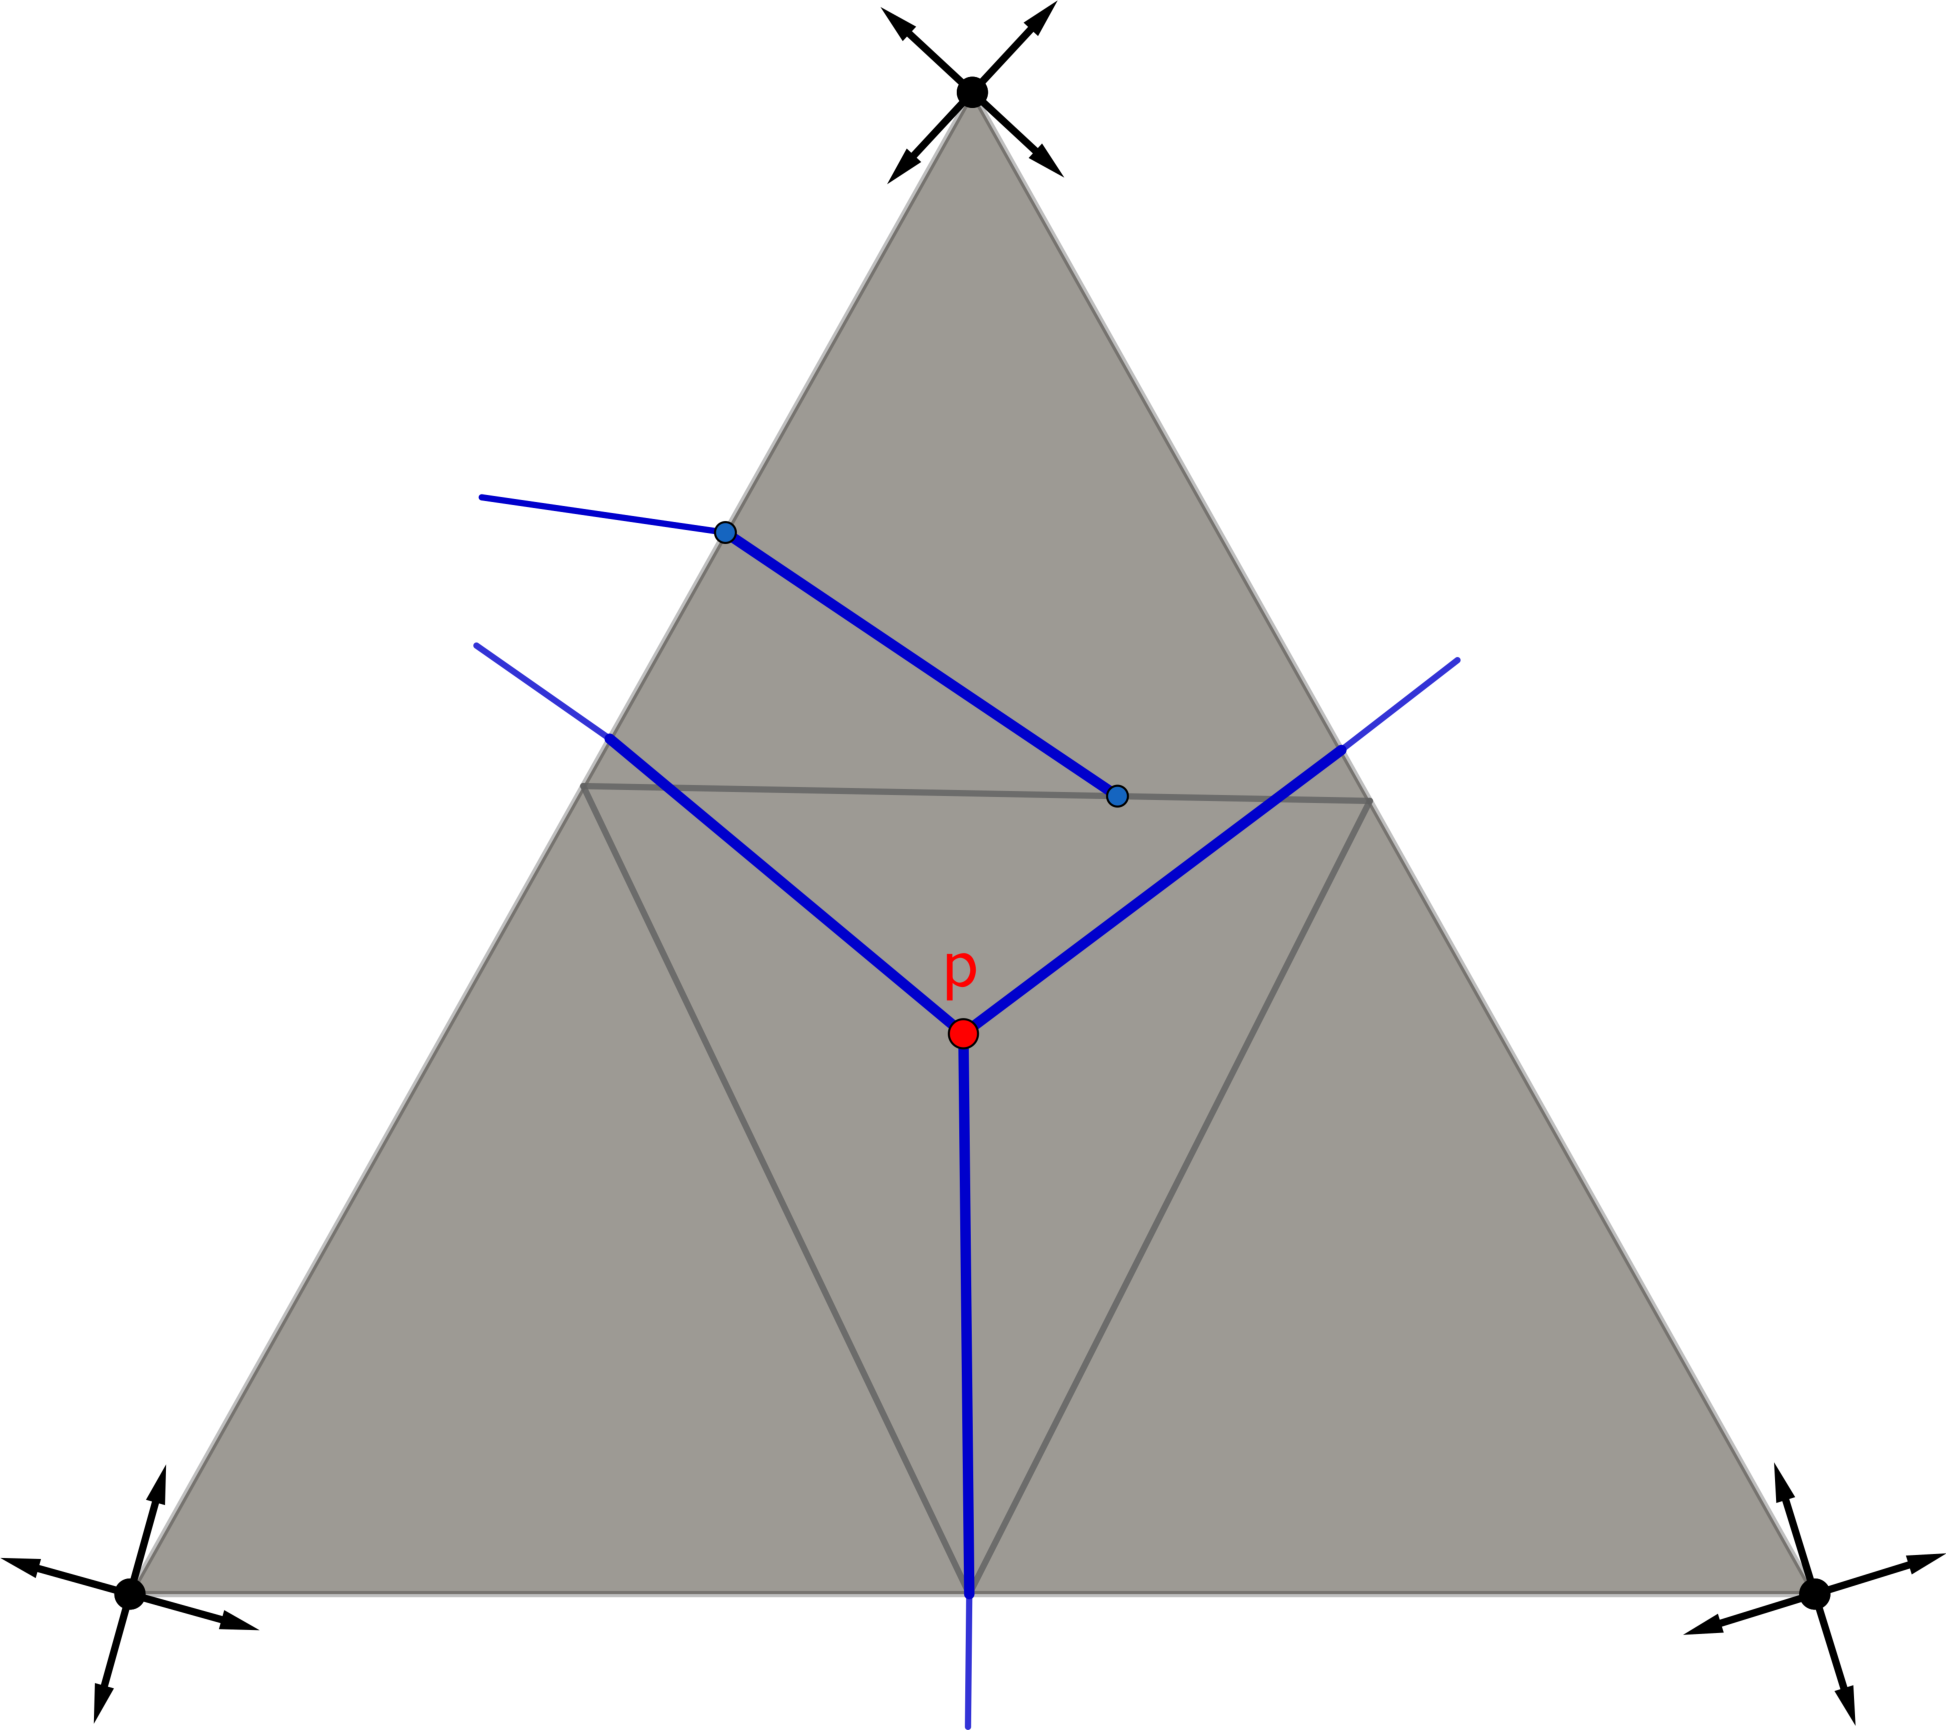
\includegraphics[width=\textwidth]{images/draw_streams_sing_2.pdf}
    \caption{Processus d'intégration d'une séparatice dans un triangle singulier: étape 1.}
    \label{fig:draw_streams_sing_2}
\end{subfigure}
\\[0.8cm]
\begin{subfigure}[b]{0.495\textwidth}
    \centering
    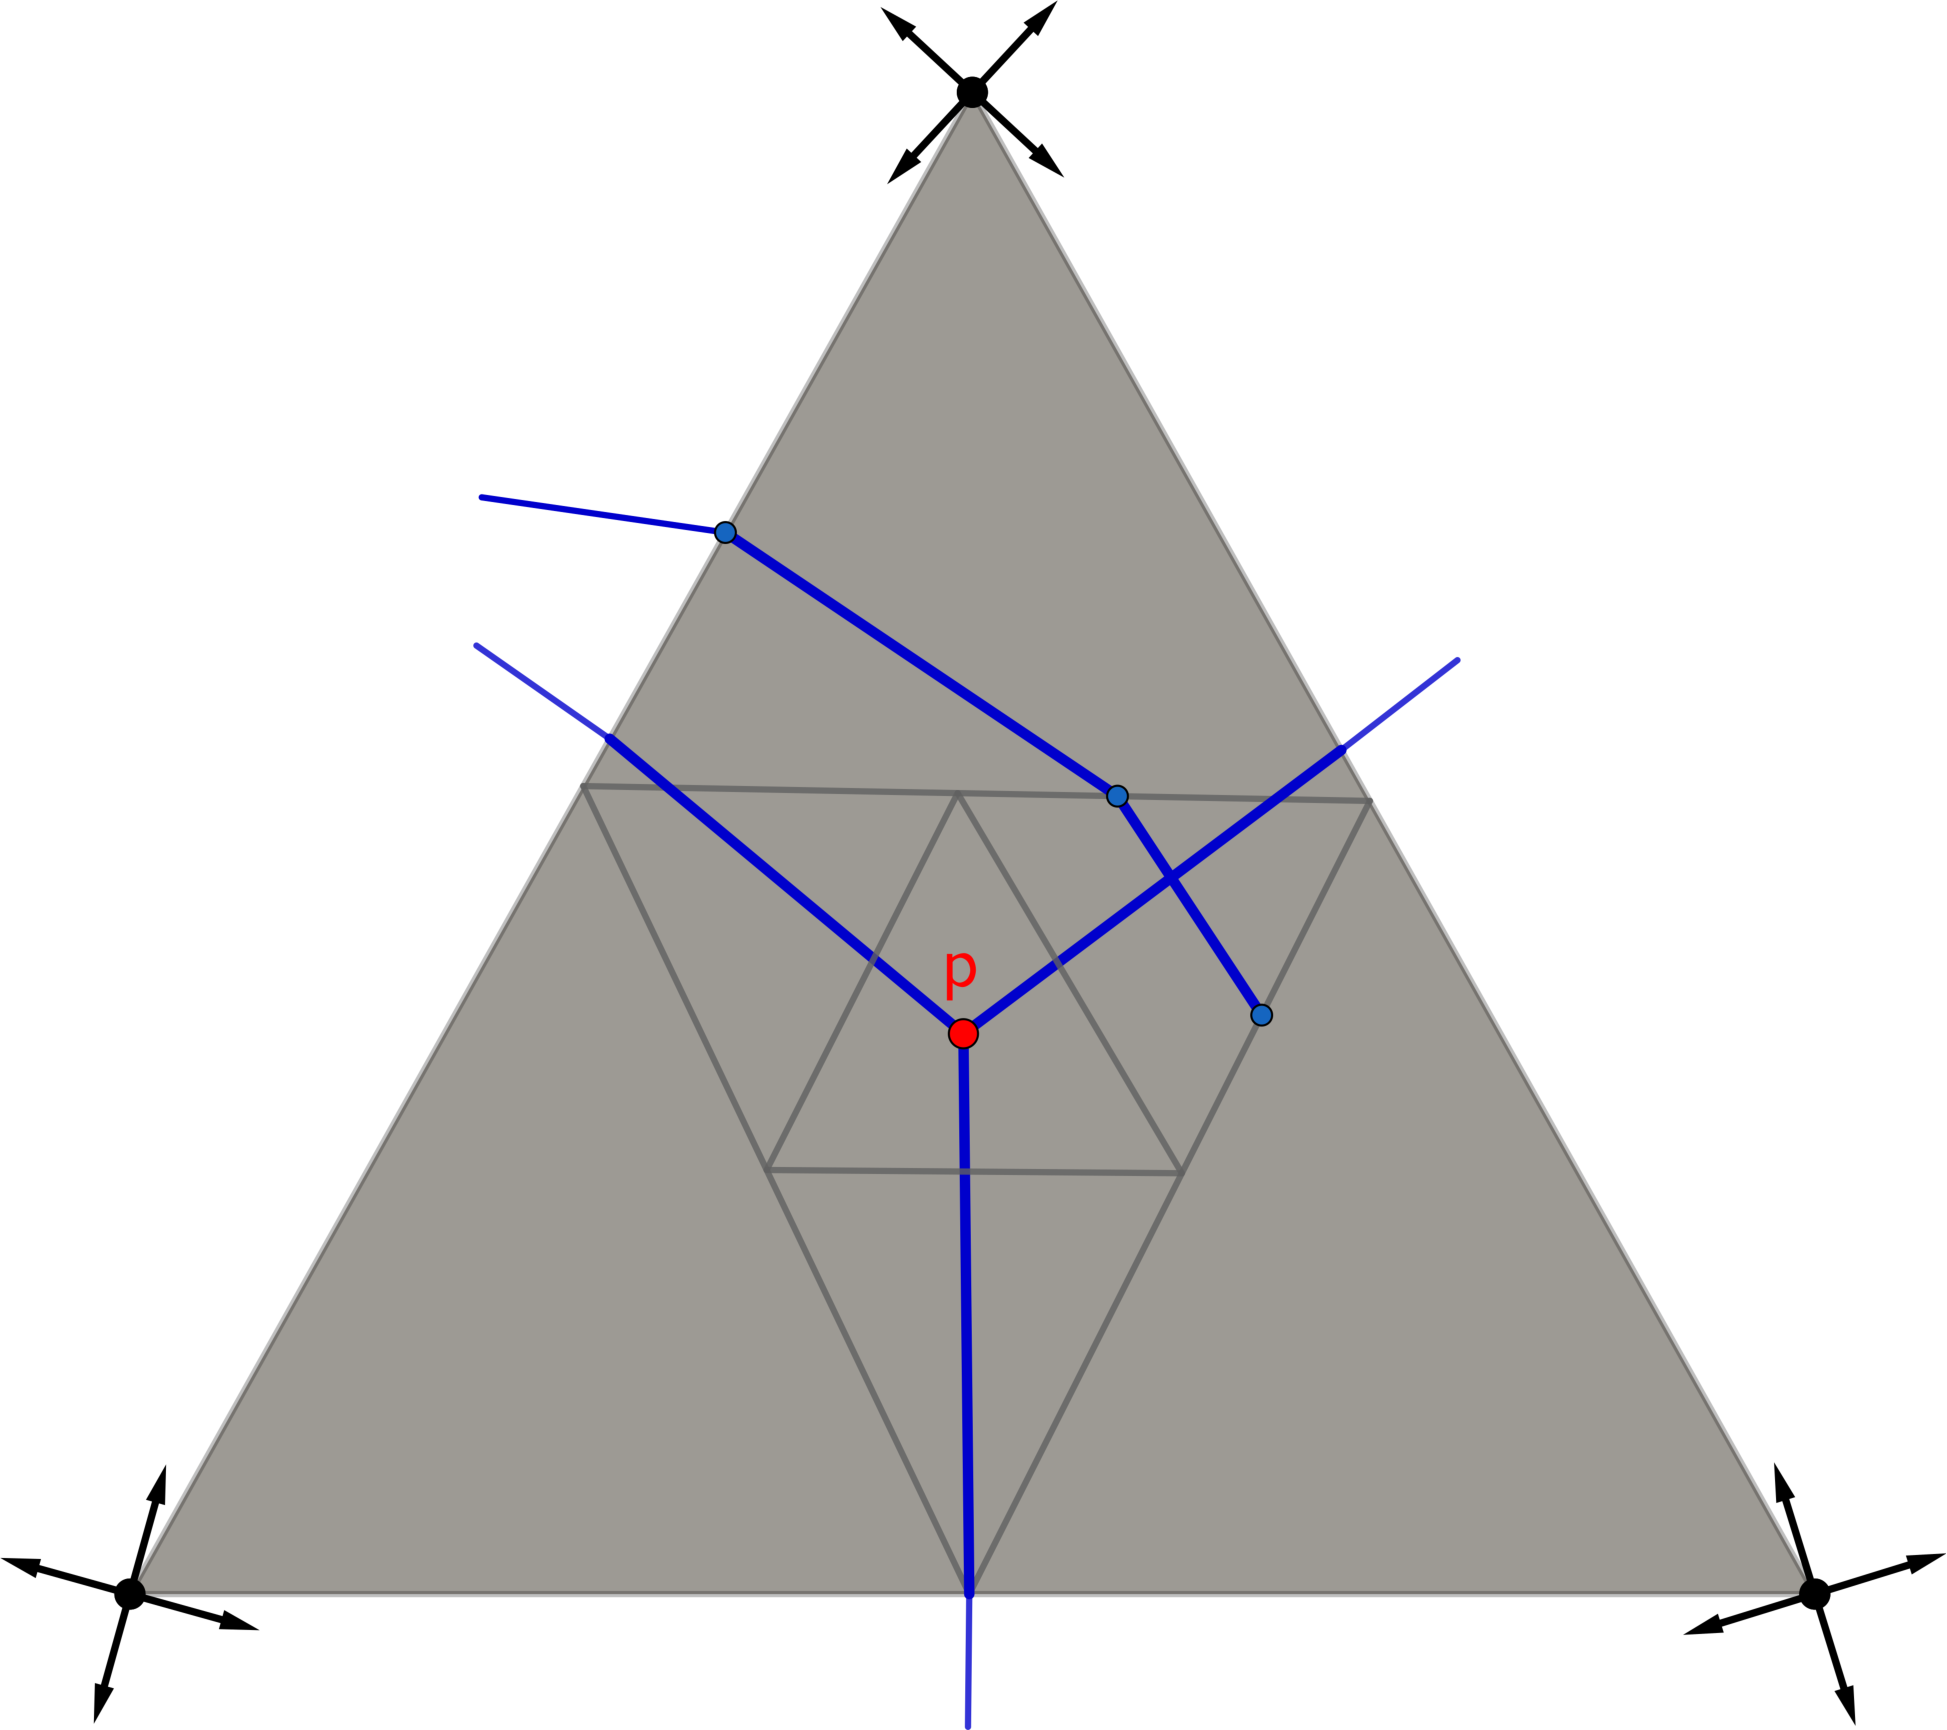
\includegraphics[width=\textwidth]{images/draw_streams_sing_3.pdf}
    \caption{Processus d'intégration d'une séparatice dans un triangle singulier: étape 2.}
    \label{fig:draw_streams_sing_3}
\end{subfigure}
\hfill
\begin{subfigure}[b]{0.495\textwidth}
    \centering
    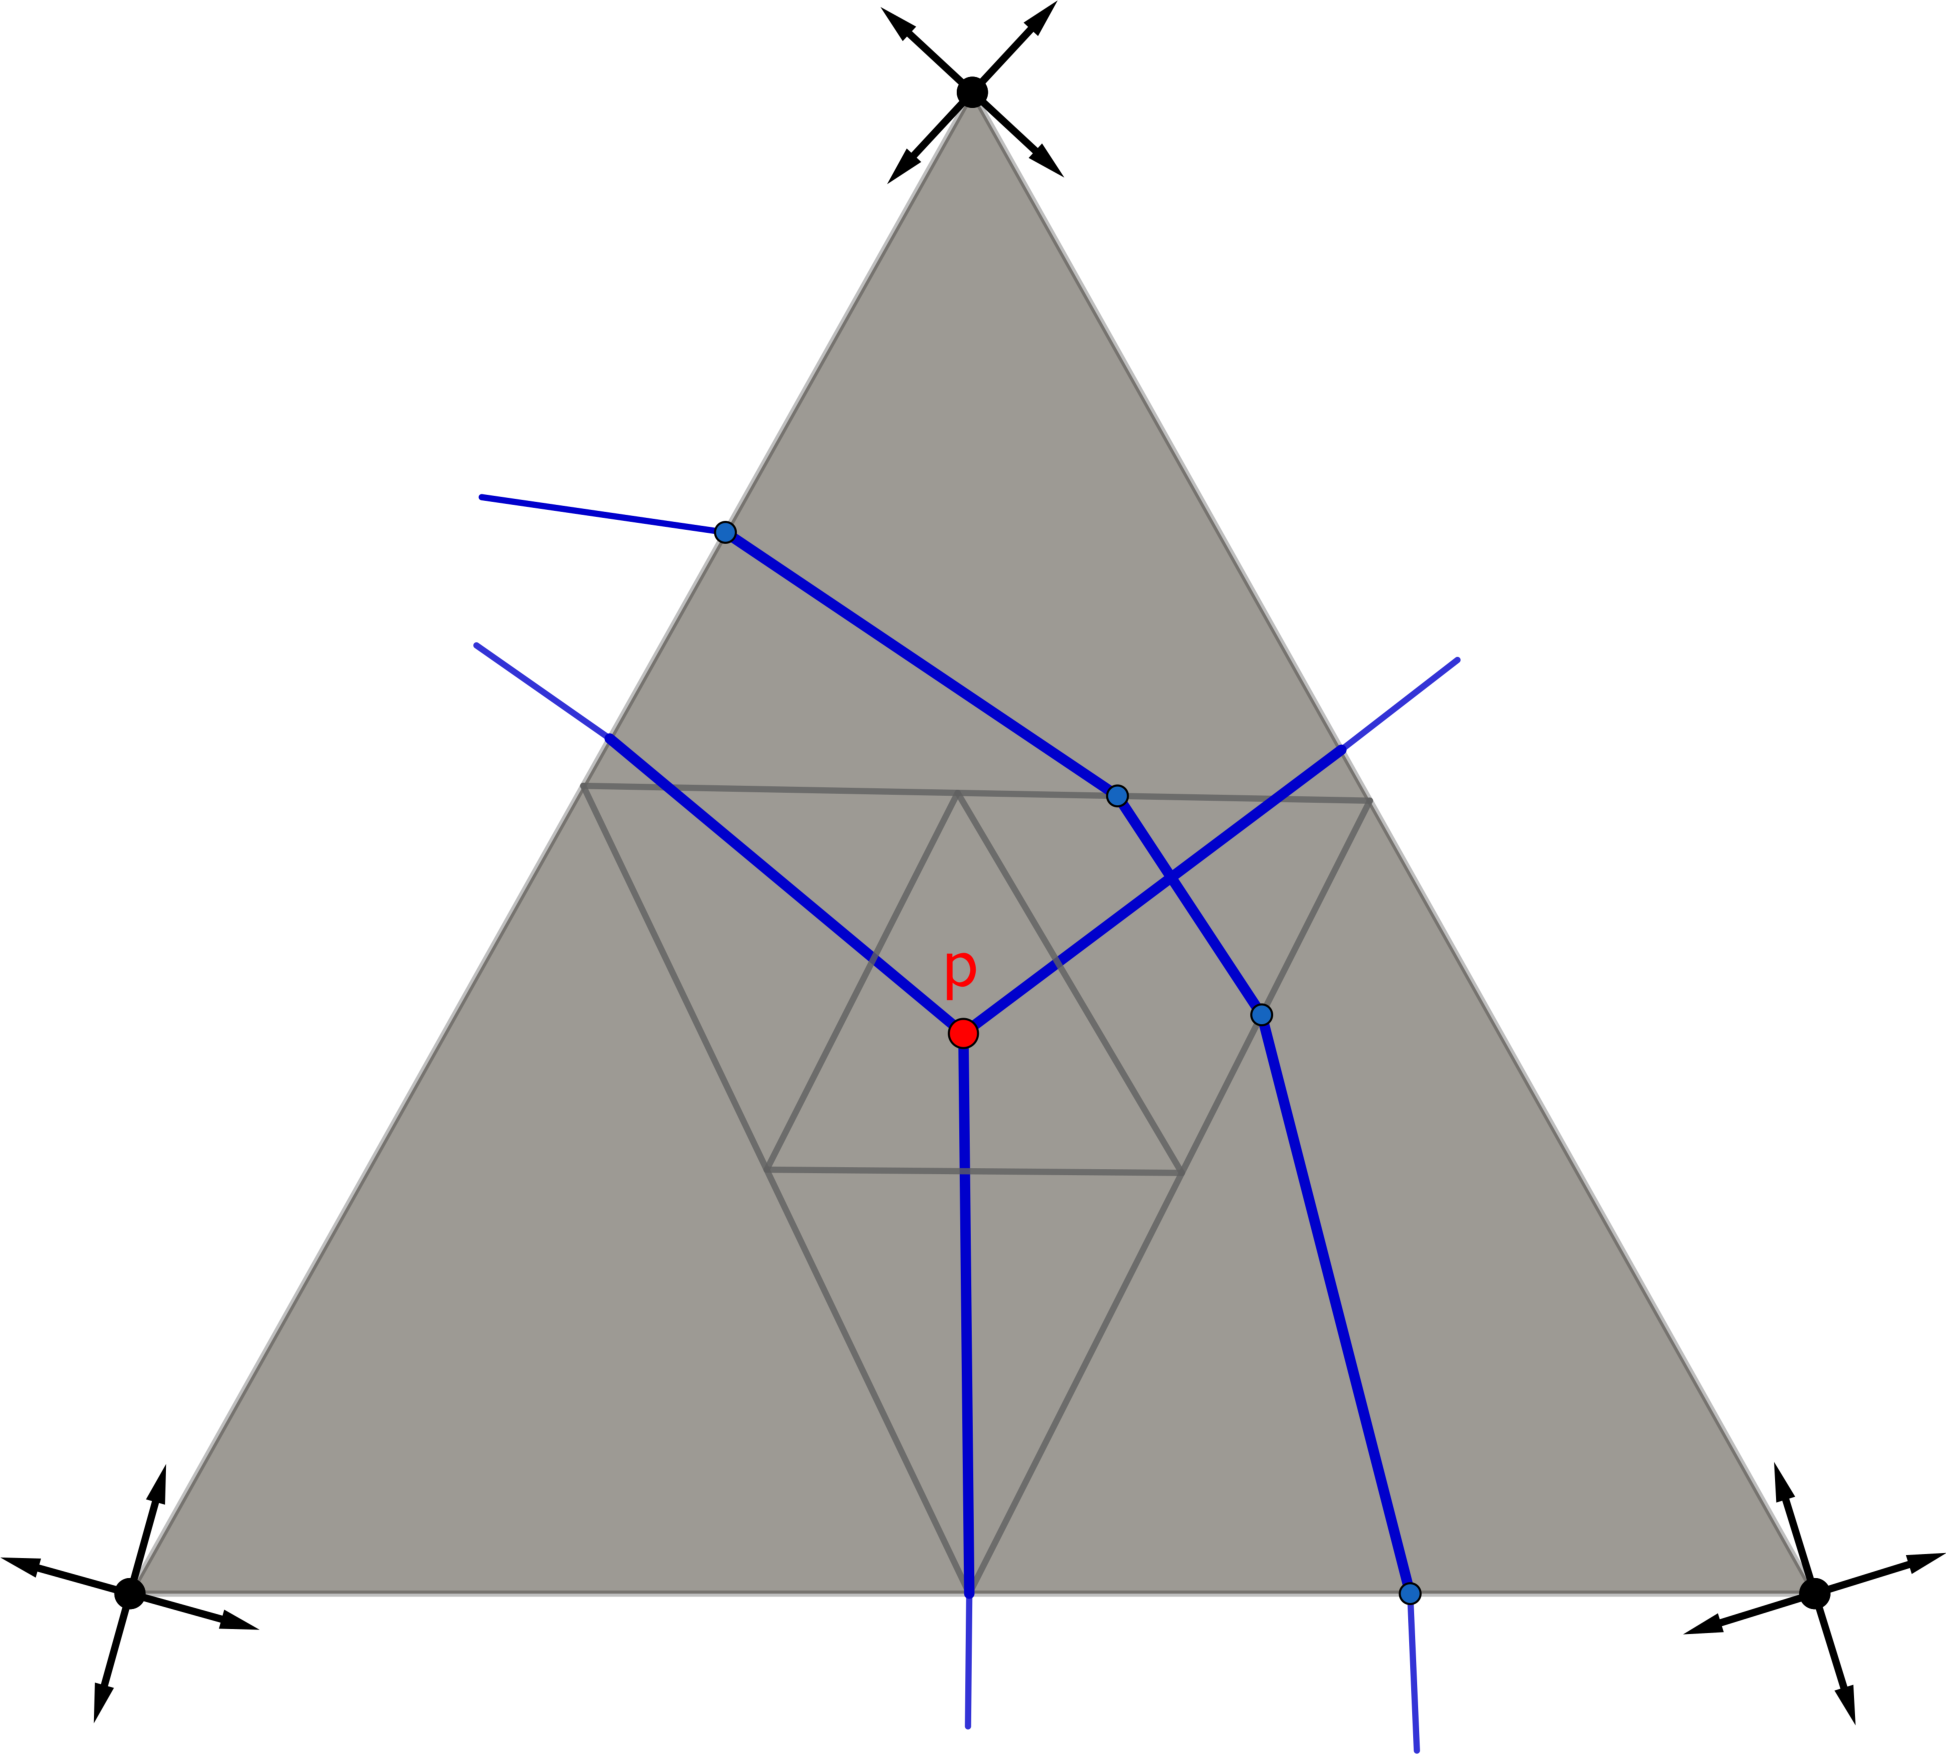
\includegraphics[width=\textwidth]{images/draw_streams_sing_4.pdf}
    \caption{Processus d'intégration d'une séparatice dans un triangle singulier: étape 3.}
    \label{fig:draw_streams_sing_4}
\end{subfigure}
\caption{Illustration de l'intégration d'une séparatice dans un triangle singulier.}
\label{fig:draw_streams_sing}
\end{figure}

\begin{figure}[!h]
\centering
\begin{subfigure}{0.65\textwidth}
    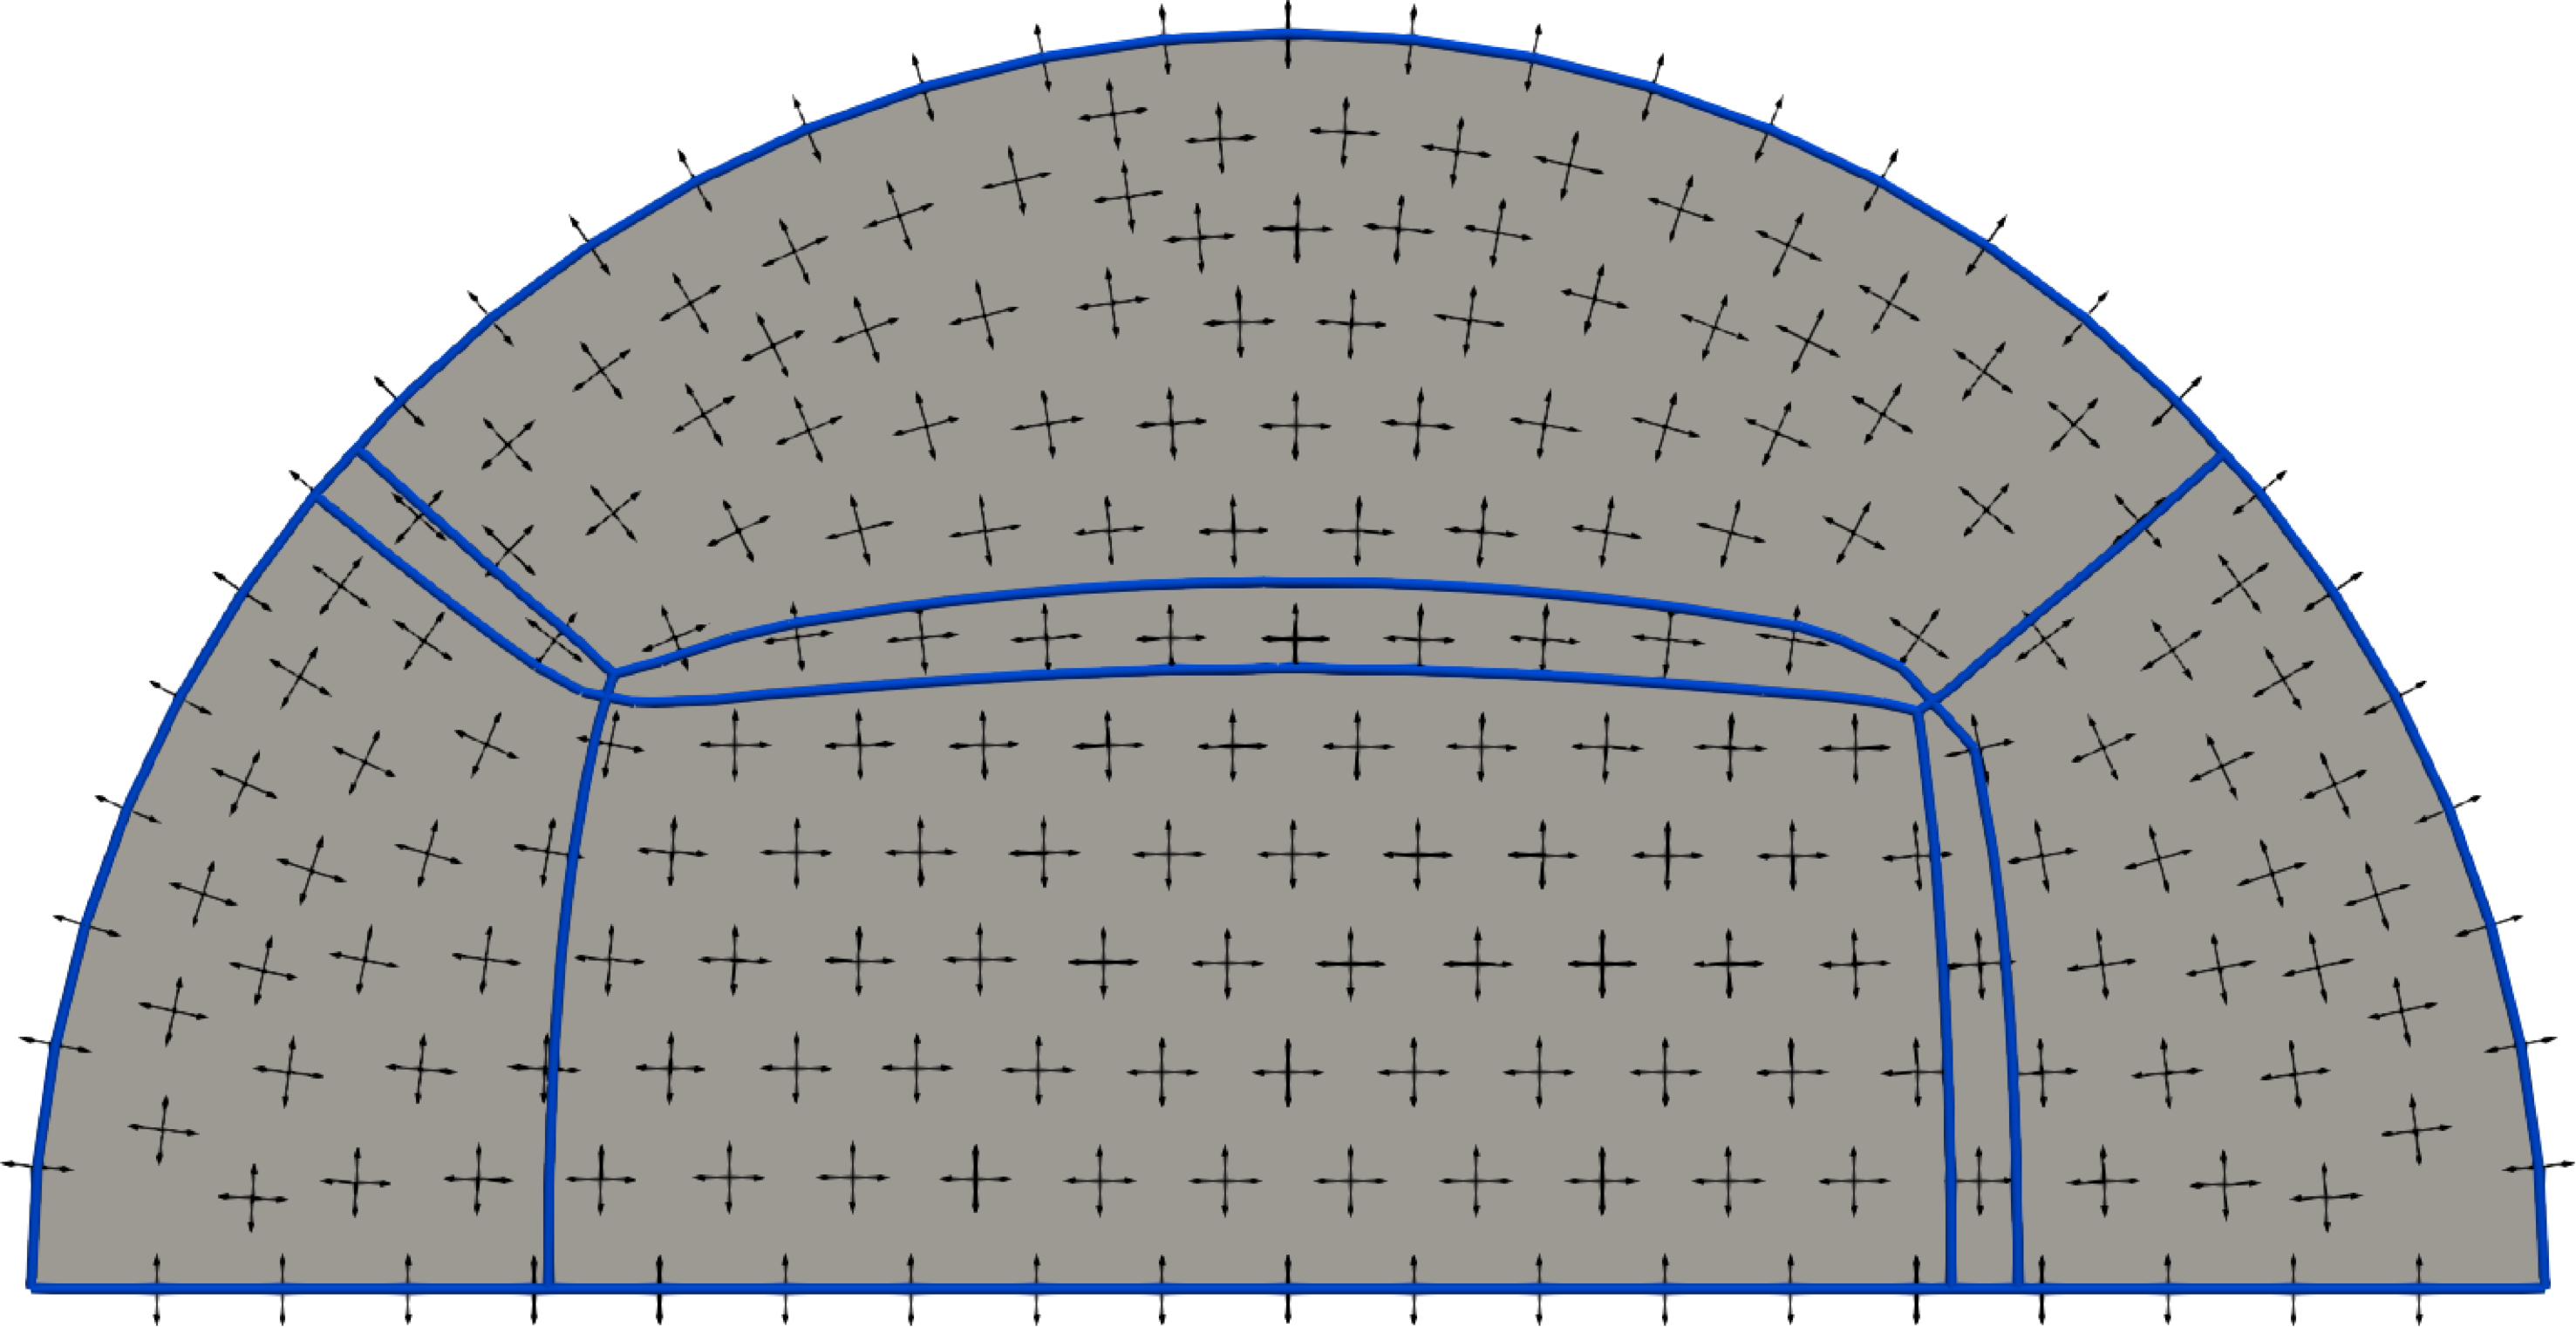
\includegraphics[width=\textwidth]{images/decoup_sans_fusion.pdf}
    \caption{Intégration de séparatrices sans fusion.}
    \label{fig:decoup_sans_fusion}
\end{subfigure}
\\[0.5cm]
\begin{subfigure}{0.65\textwidth}
    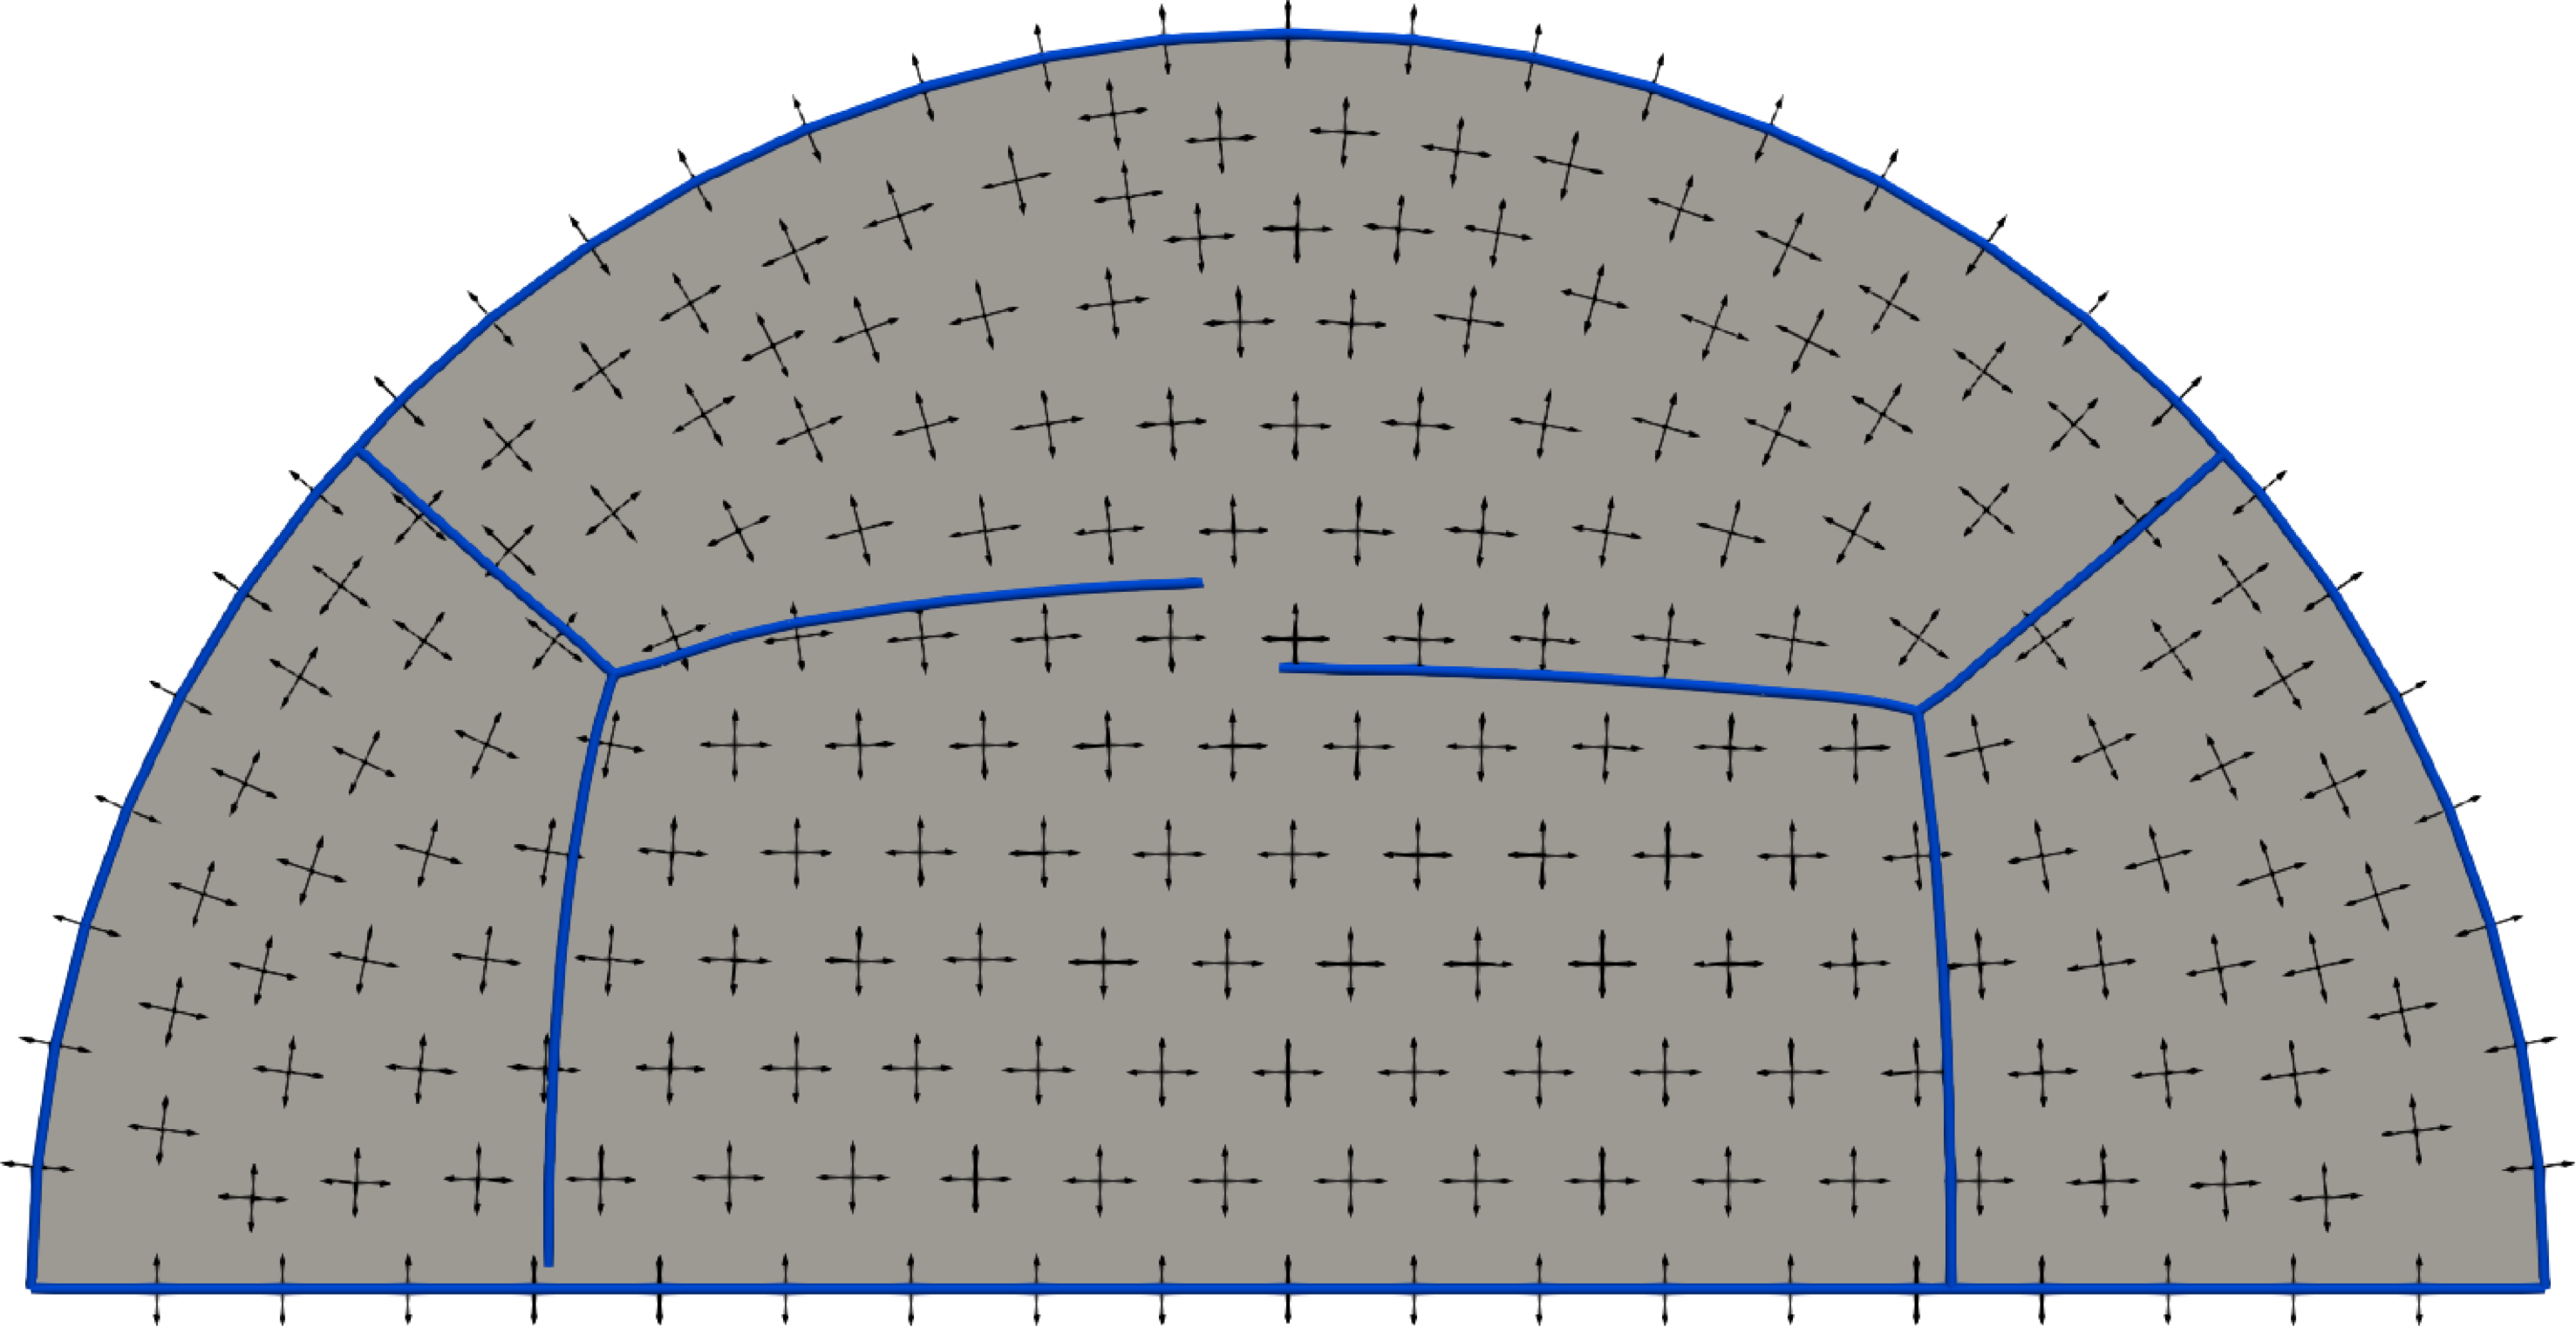
\includegraphics[width=\textwidth]{images/decoup_detect_fusion.pdf}
    \caption{Détection d'une fusion.}
    \label{fig:decoup_detect_fusion}
\end{subfigure}
\\[0.5cm]
\begin{subfigure}{0.65\textwidth}
    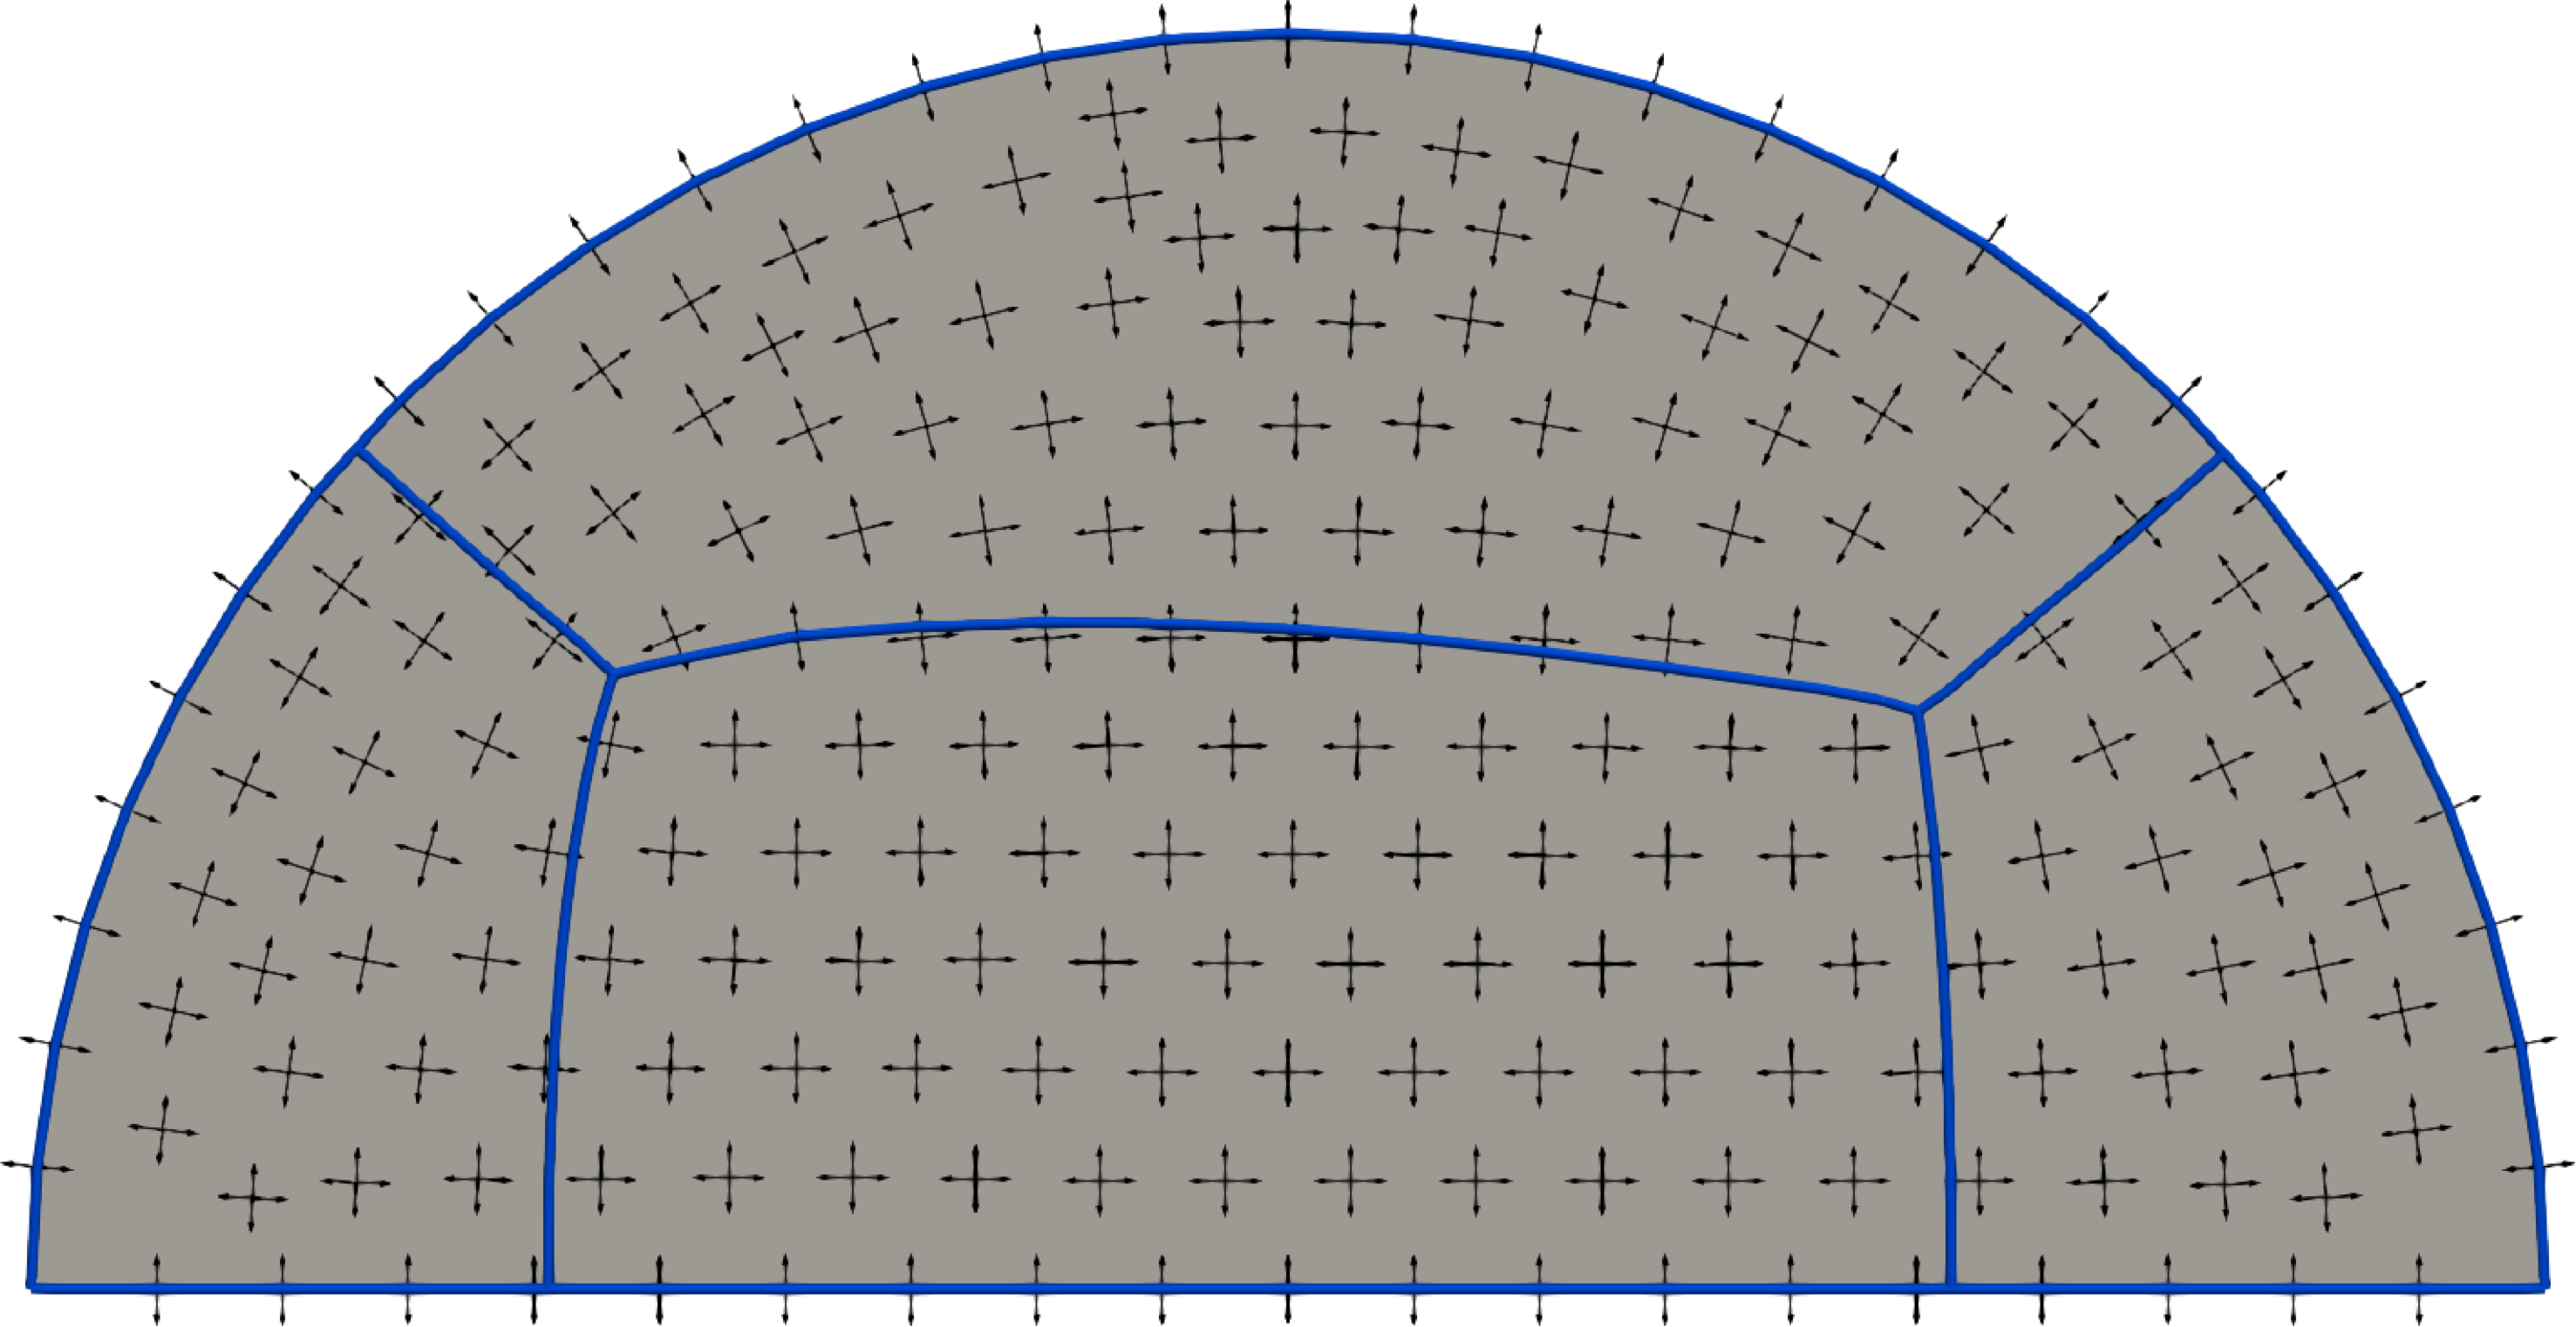
\includegraphics[width=\textwidth]{images/decoup_fusion.pdf}
    \caption{Intégration de séparatrices avec fusion.}
    \label{fig:decoup_fusion}
\end{subfigure}
\caption{Illustration de la fusion de séparatrices.}
\label{fig:fusion}
\end{figure}

Lors de l'intégration d'une séparatrice, il peut arriver qu'elle doive traverser un triangle singulier. Dans ce cas, le processus d'intégration tel que décrit précédemment peut échouer (voir la figure \ref{fig:draw_streams_sing_1}) en ne capturant pas correctement les intersections avec les autres séparatrices. Cela résulte du fait que le champ d'angle associé au champ de croix dans le triangle n'est pas continu et présente des variations importantes. Pour surmonter ce problème, nous cherchons à représenter la séparatrice dans le triangle singulier en utilisant une succession d'autres segments calculés par un raffinement local du maillage à l'intérieur du triangle singulier. L'objectif est d'isoler le point singulier par rapport à la trajectoire de la séparatrice. Voici le procédé :

Considérons $T$ comme un triangle contenant un point singulier que doit être traversé par une séparatrice dont l'origine ne se trouve pas dans $T$. En d'autres termes, le dernier point calculé lors de la construction de cette séparatrice appartient à $T$ et le processus habituel d'intégration a généré un segment traversant $T$ (voir figure \ref{fig:draw_streams_1}). Dans la suite, nous appellerons ce "dernier point" le point d'entrée de la séparatrice dans $T$.

On commence par subdiviser $T$ en quatre triangles. Cette subdivision peut être réalisée en reliant, par exemple, les milieux des arêtes de $T$. Il est essentiel de noter que si le point d'entrée coïncide avec le milieu d'une arête, un autre point de cette arête doit être choisi pour la subdivision. L'objectif est que le point d'entrée se retrouve associé à un triangle issu de la subdivision ne contenant pas de point singulier. On peut alors appliquer le processus d'intégration dans ce triangle, tel que décrit précédemment (voir figure \ref{fig:draw_streams_sing_2}).

Il ne reste plus qu'à itérer ce schéma de construction jusqu'à ce que la séparatrice sorte de la partie du plan correspondant au triangle initial (voir figures \ref{fig:draw_streams_sing_3} et \ref{fig:draw_streams_sing_4}). On se retrouve ainsi avec un raffinement local et adapté du maillage en fonction de la trajectoire de la séparatrice, ce qui permet en pratique de ne pas raffiner l'intégralité du maillage pour avoir une bonne approximation de la séparatrice. Il convient de souligner qu'il n'est pas nécessaire d'apporter des modifications locales au maillage dans sa globalité. Après avoir construit la séparatrice, nous conservons uniquement ses points de passage et supprimons tout raffinement local utilisé.

\paragraph{Fusion de séparatrices:}

de manière similaire à ce qui est réalisé dans \cite{marcon2019high}, les séparatrices du champ de croix sont construites simultanément en incrémentant chacune d'elles progressivement, et la rencontre entre deux séparatrices est anticipée en comparant à chaque incrément, d'une part, la distance entre les derniers points calculés et, d'autre part, les directions des derniers segments construits. En d'autres termes, on cherche à déterminer si, à un moment donné, deux séparatrices données avancent dans des directions opposées et si elles sont suffisamment proches l'une de l'autre. On compare ces deux mesures à des seuils prédéfinis, et en fonction du résultat, on décide de fusionner ou non les deux séparatrices.

La fusion se réalise en créant une nouvelle séparatrice par une fusion linéaire des points des deux séparatrices impliquées. Pour ce faire, chaque séparatrice est prolongée à travers $\Omega_h$ jusqu'à atteindre la position de départ de l'autre. Les deux séparatrices sont ensuite rediscrétisées avec un même nombre de points. L'intérêt de fusionner les séparatrices réside dans la réduction de leur nombre, ce qui se traduit directement par une diminution du nombre de régions générées lors du découpage du domaine. Nous illustrons la fusion de deux séparatrices sur la figure \ref{fig:fusion}. Il est remarquable que la non-fusion des séparatrices n'empêche par d'avoir un partitionnement à 4 côtés mais génère davantage de régions, certaines étant fortement étirées et non homogènes par rapport aux autres, ce qui est une source potentielle d'inhomogénéité des mailles dans les maillages quadrilatéraux.

\begin{figure}[h!]
\centering
\begin{subfigure}{0.49\textwidth}
    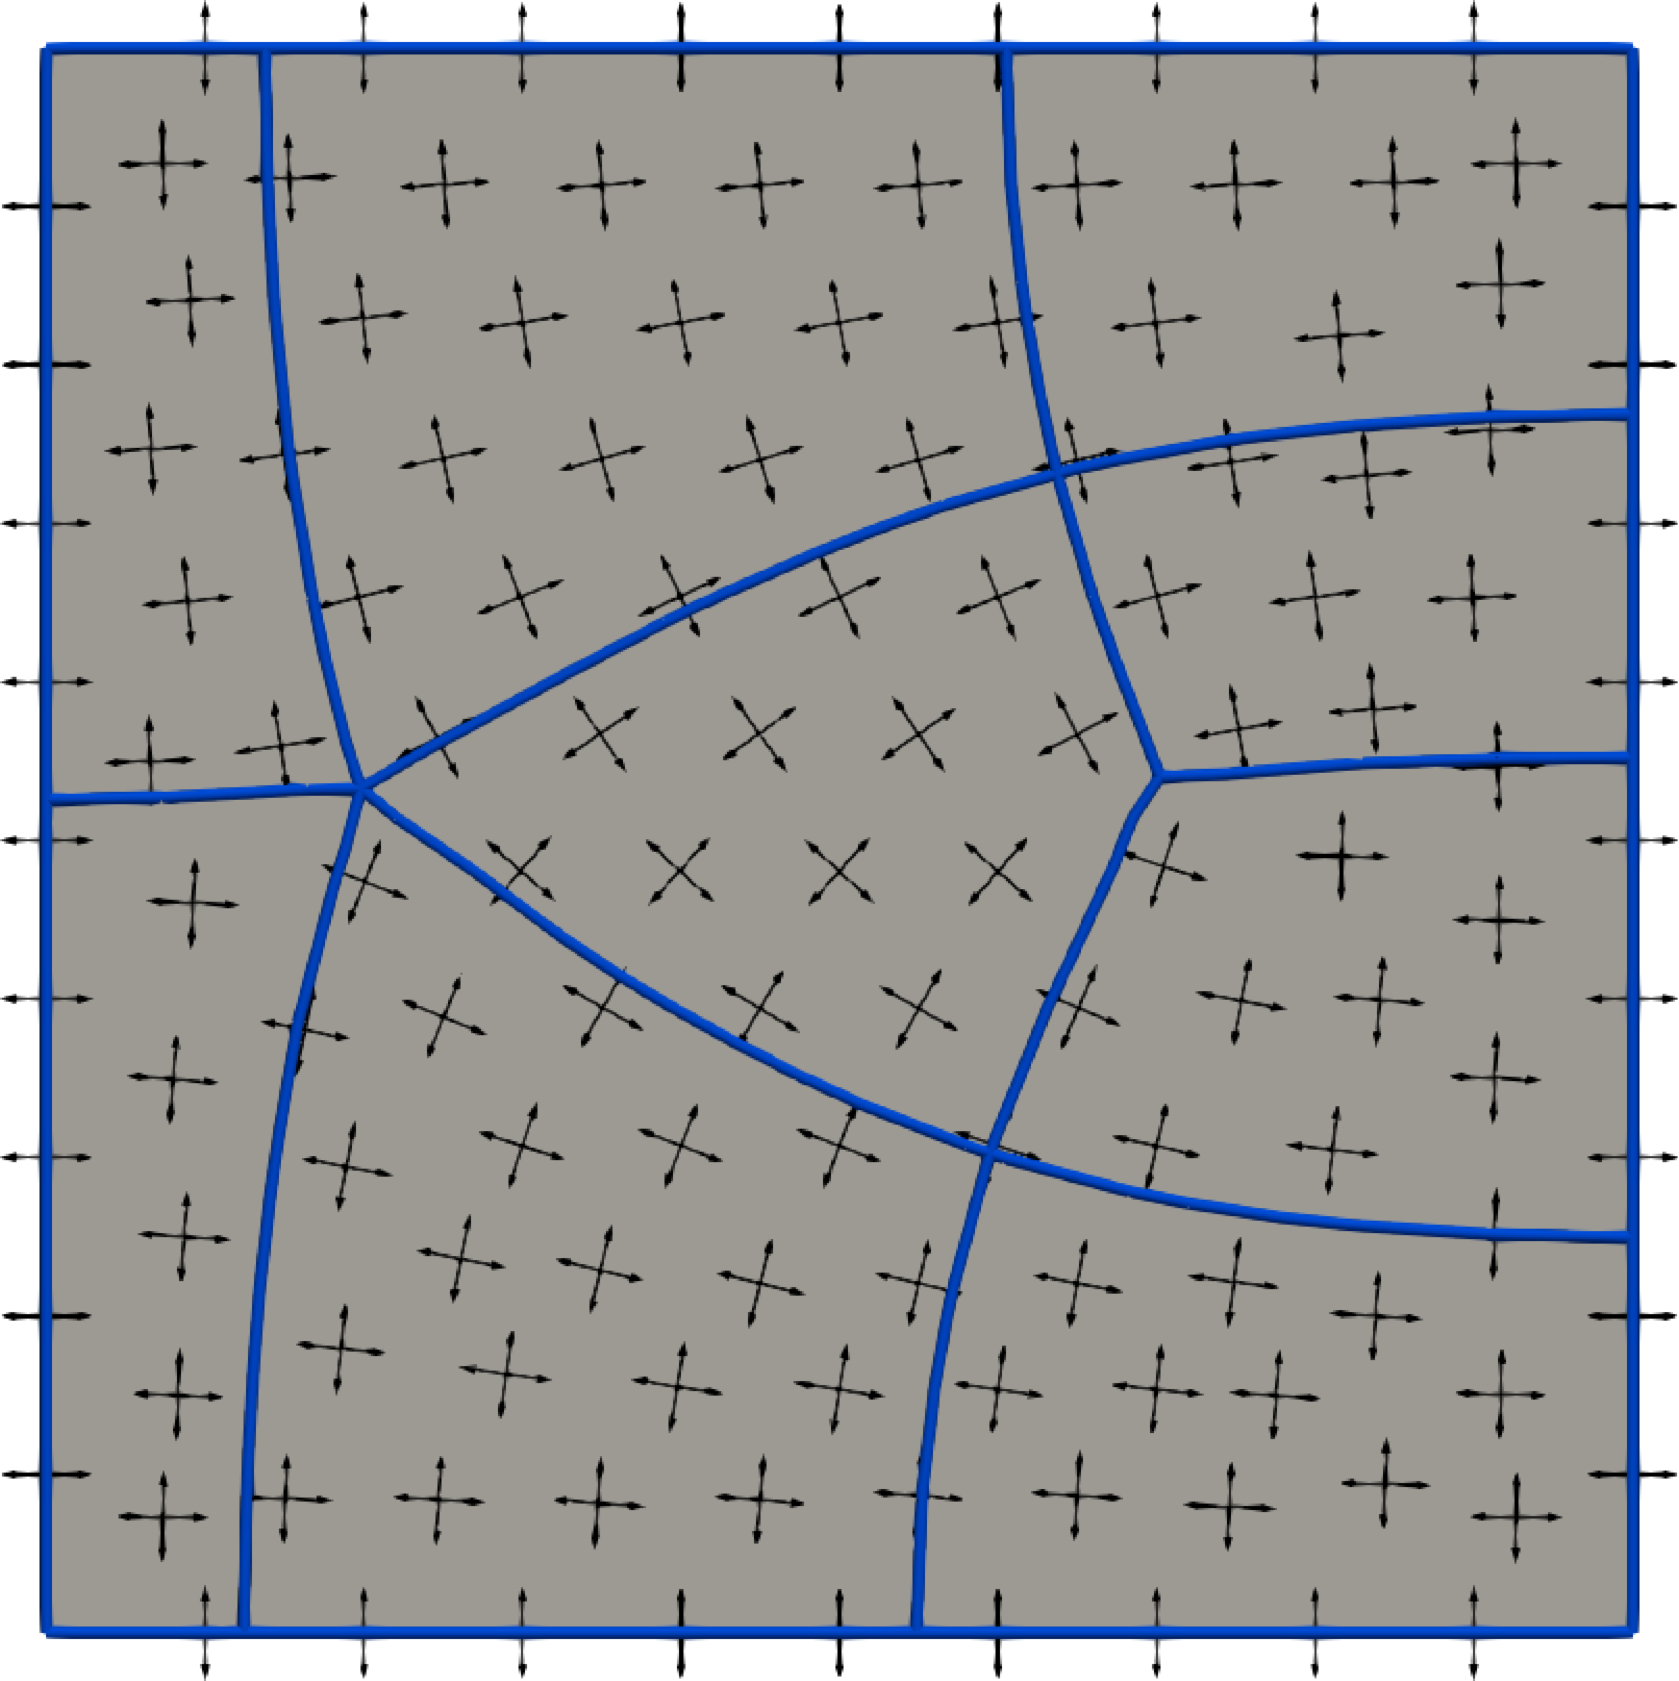
\includegraphics[width=\textwidth]{images/eclatement_1.pdf}
    %\caption{Insertion de $D$.}
    %\label{fig:quad_eclatement}
\end{subfigure}
\hfill
\begin{subfigure}{0.49\textwidth}
    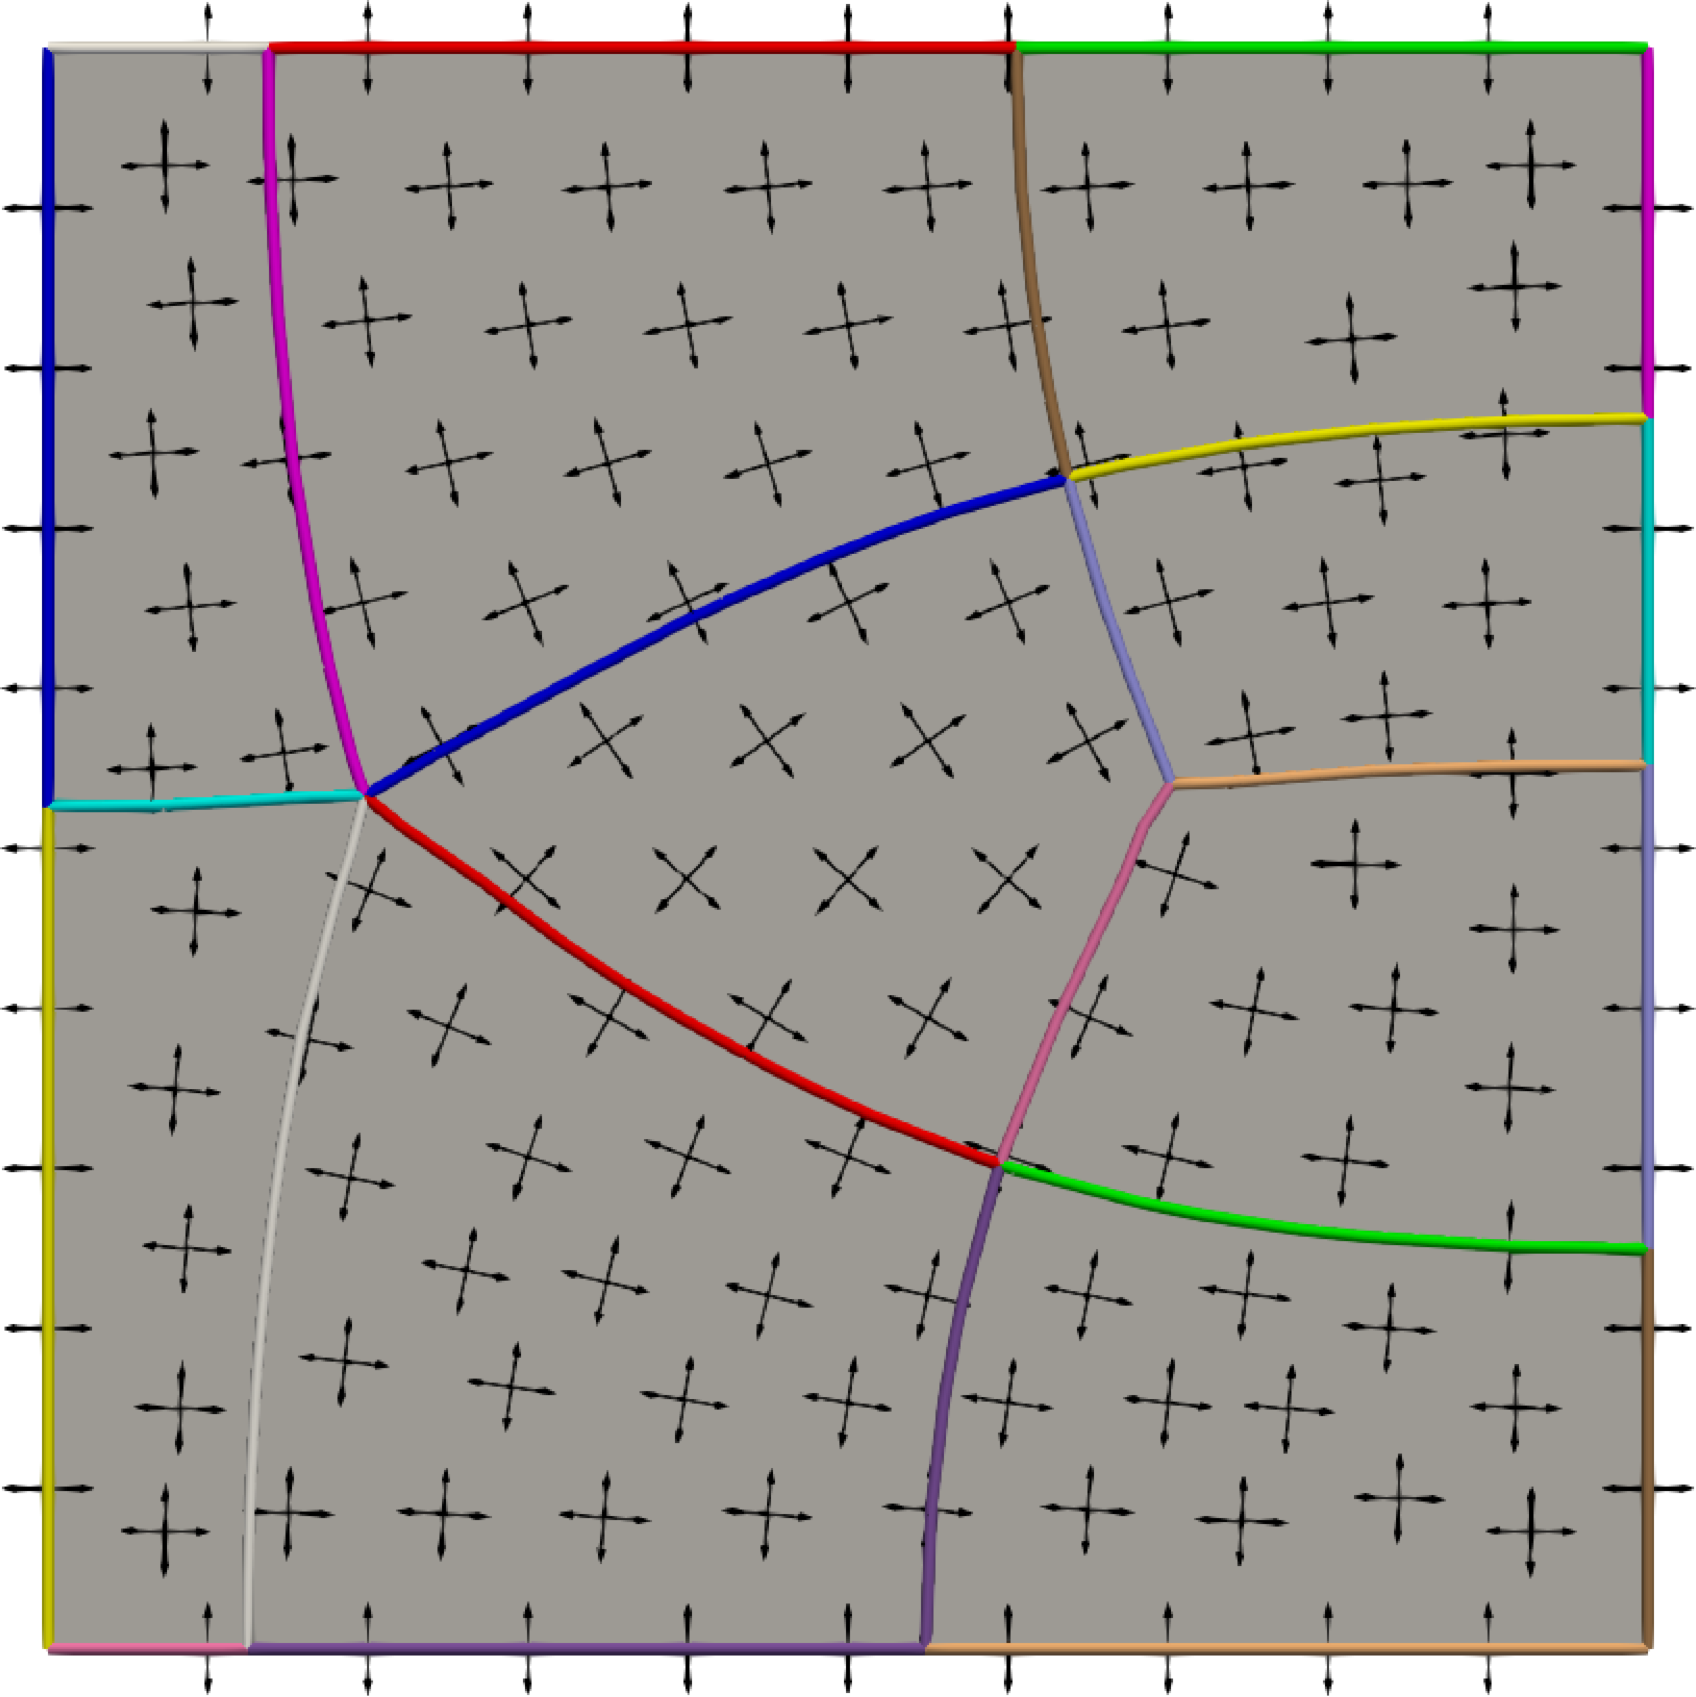
\includegraphics[width=\textwidth]{images/intersect_stream.pdf}
    %\caption{Insertion de $E$.}
    %\label{fig:quad_carre}
\end{subfigure}
\caption{Intersection de séparatrices.}
\label{fig:detect_intersection}
\end{figure}


\subsection{Assemblage des partitions}

Une fois les séparatrices construites, nous procédons à la subdivision du maillage triangulaire $\Omega_h$ en plusieurs régions distinctes. Cette opération consiste à modifier $\Omega_h$ en y intégrant les segments formant les séparatrices, créant ainsi un nouveau maillage. Notre objectif est de délimiter chaque région sous forme de sous-maillage distinct de $\Omega_h$ ce qui facilite la génération de maillage quadrilatéral sur chaque partition (voir la section \ref{sec:gen_mesh_quad}). Ce processus débute par l'identification des frontières de ces régions via la localisation des points d'intersection entre les séparatrices, suivie de l'extraction de chaque région individuelle.

\paragraph{Intersections de séparatrices:}

Comme annoncé, la première étape de ce processus consiste à déterminer les frontières des régions. La recherche des points d'intersection entre les séparatrices peut être réalisée localement dans chaque triangle et simultanément. Étant donné que les séparatrices sont constituées de segments, il suffit de vérifier l'intersection de ces segments les uns par rapport aux autres. En découpant les séparatrices au niveau de ces points d'intersection, cela met en évidence les contours des régions, comme illustré sur la figure \ref{fig:detect_intersection} avec une couleur différente pour chaque séparatice.

\paragraph{Identification des partitions:}
Dans cette phase, notre objectif est de découper le maillage triangulaire initial $\Omega_h$ en plusieurs sous-maillages, représentant chacun une partition. Pour y parvenir, nous enrichissons $\Omega_h$ en y insérant les points qui constituent les séparatrices, puis nous ajustons le maillage pour qu'il intègre les segments formés par ces séparatrices. Cette étape de modification du maillage peut être réalisée localement au niveau de chaque triangle de $\Omega_h$, exploitant ainsi les capacités de calcul parallèle pour accélérer le processus.

Considérons $T$ comme un triangle de $\Omega_h$ traversé par certains segments des séparatrices construites (voir figure \ref{fig:exemple_insert_pt_0}). Pour insérer ces segments dans $T$, nous commençons par introduire les points de bord de ces segments tout en conservant la structure en triangles du triangle initial. De cette manière, nous obtenons un raffinement triangulaire de $T$. Pour insérer un point $p$ dans $T$ (s'il ne fait pas encore parti du raffinement), on commence par identifier l'élément ou les deux éléments de $T$ contenant ce point. Ensuite, l'insertion de $p$ s'opère dans ces éléments en générant de nouveaux triangles de la manière suivante (voir figure \ref{fig:insert_pt}):\\
\begin{itemize}
 \item si $p$ se trouve à l'intérieur d'un triangle $K\subset T$ alors son insertion génère trois nouveaux triangles par liaison de $p$ aux sommets de $K$.\\
 \item si $p$ se trouve sur une arête d'un triangle $K\subset T$, alors son insertion engendre deux nouveaux triangles par liaison de $p$ au sommet opposé à l'arête concernée.\\
\end{itemize}

\begin{figure}[h!]
\centering
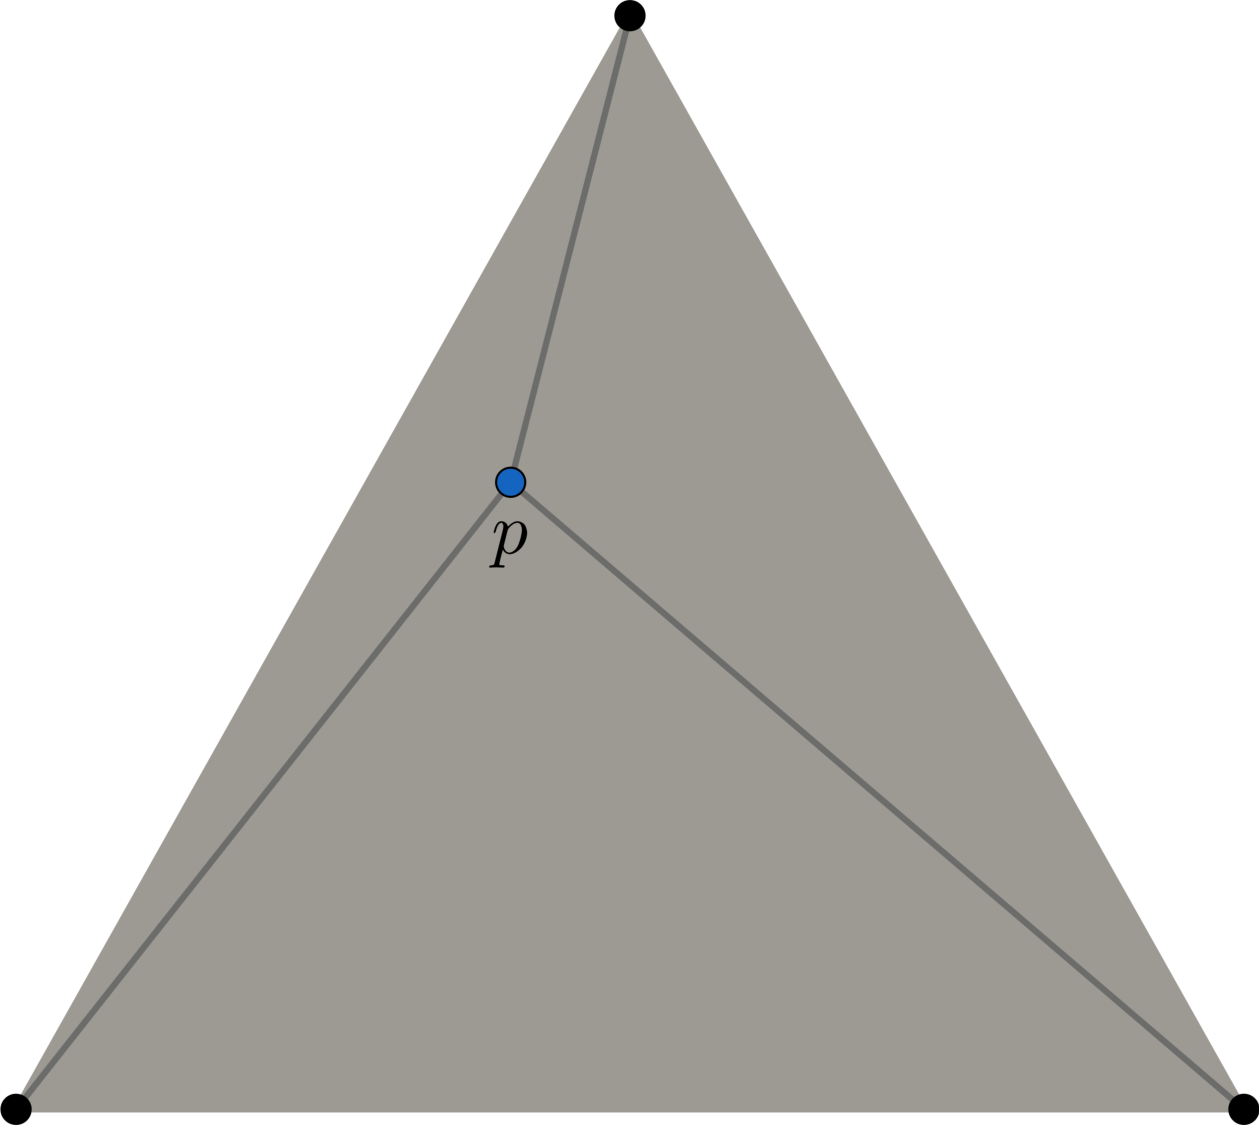
\includegraphics[scale=0.37]{images/insert_pt_1.pdf}\hfill
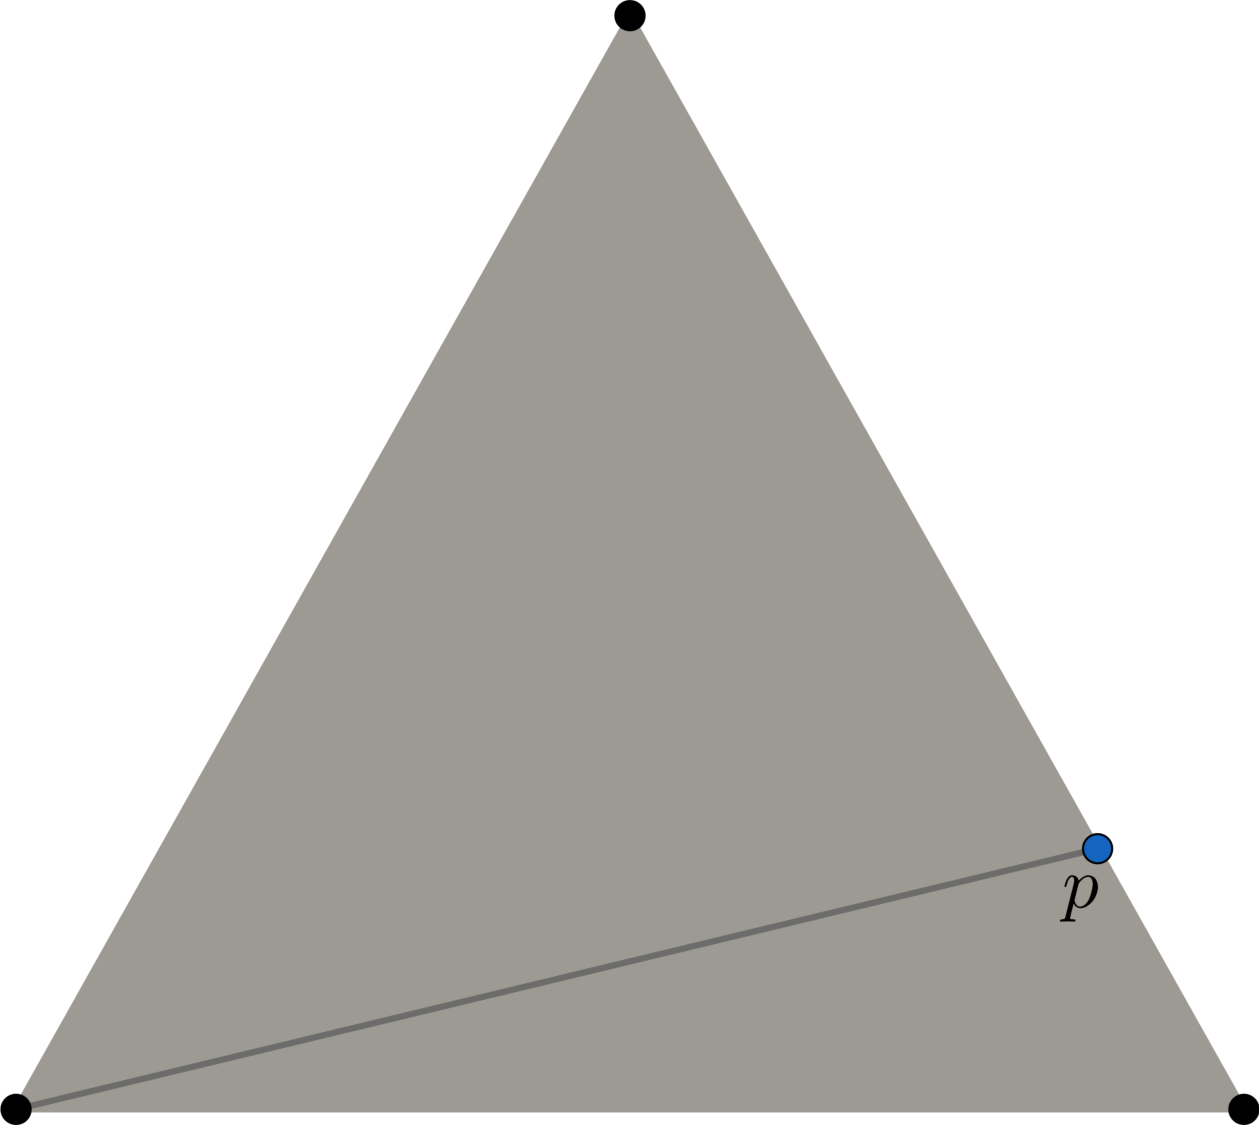
\includegraphics[scale=0.37]{images/insert_pt_2.pdf}
\caption{Insertion d'un point dans un triangle.}
\label{fig:insert_pt}
\end{figure}

\begin{figure}[h!]
\centering
\begin{subfigure}{0.45\textwidth}
    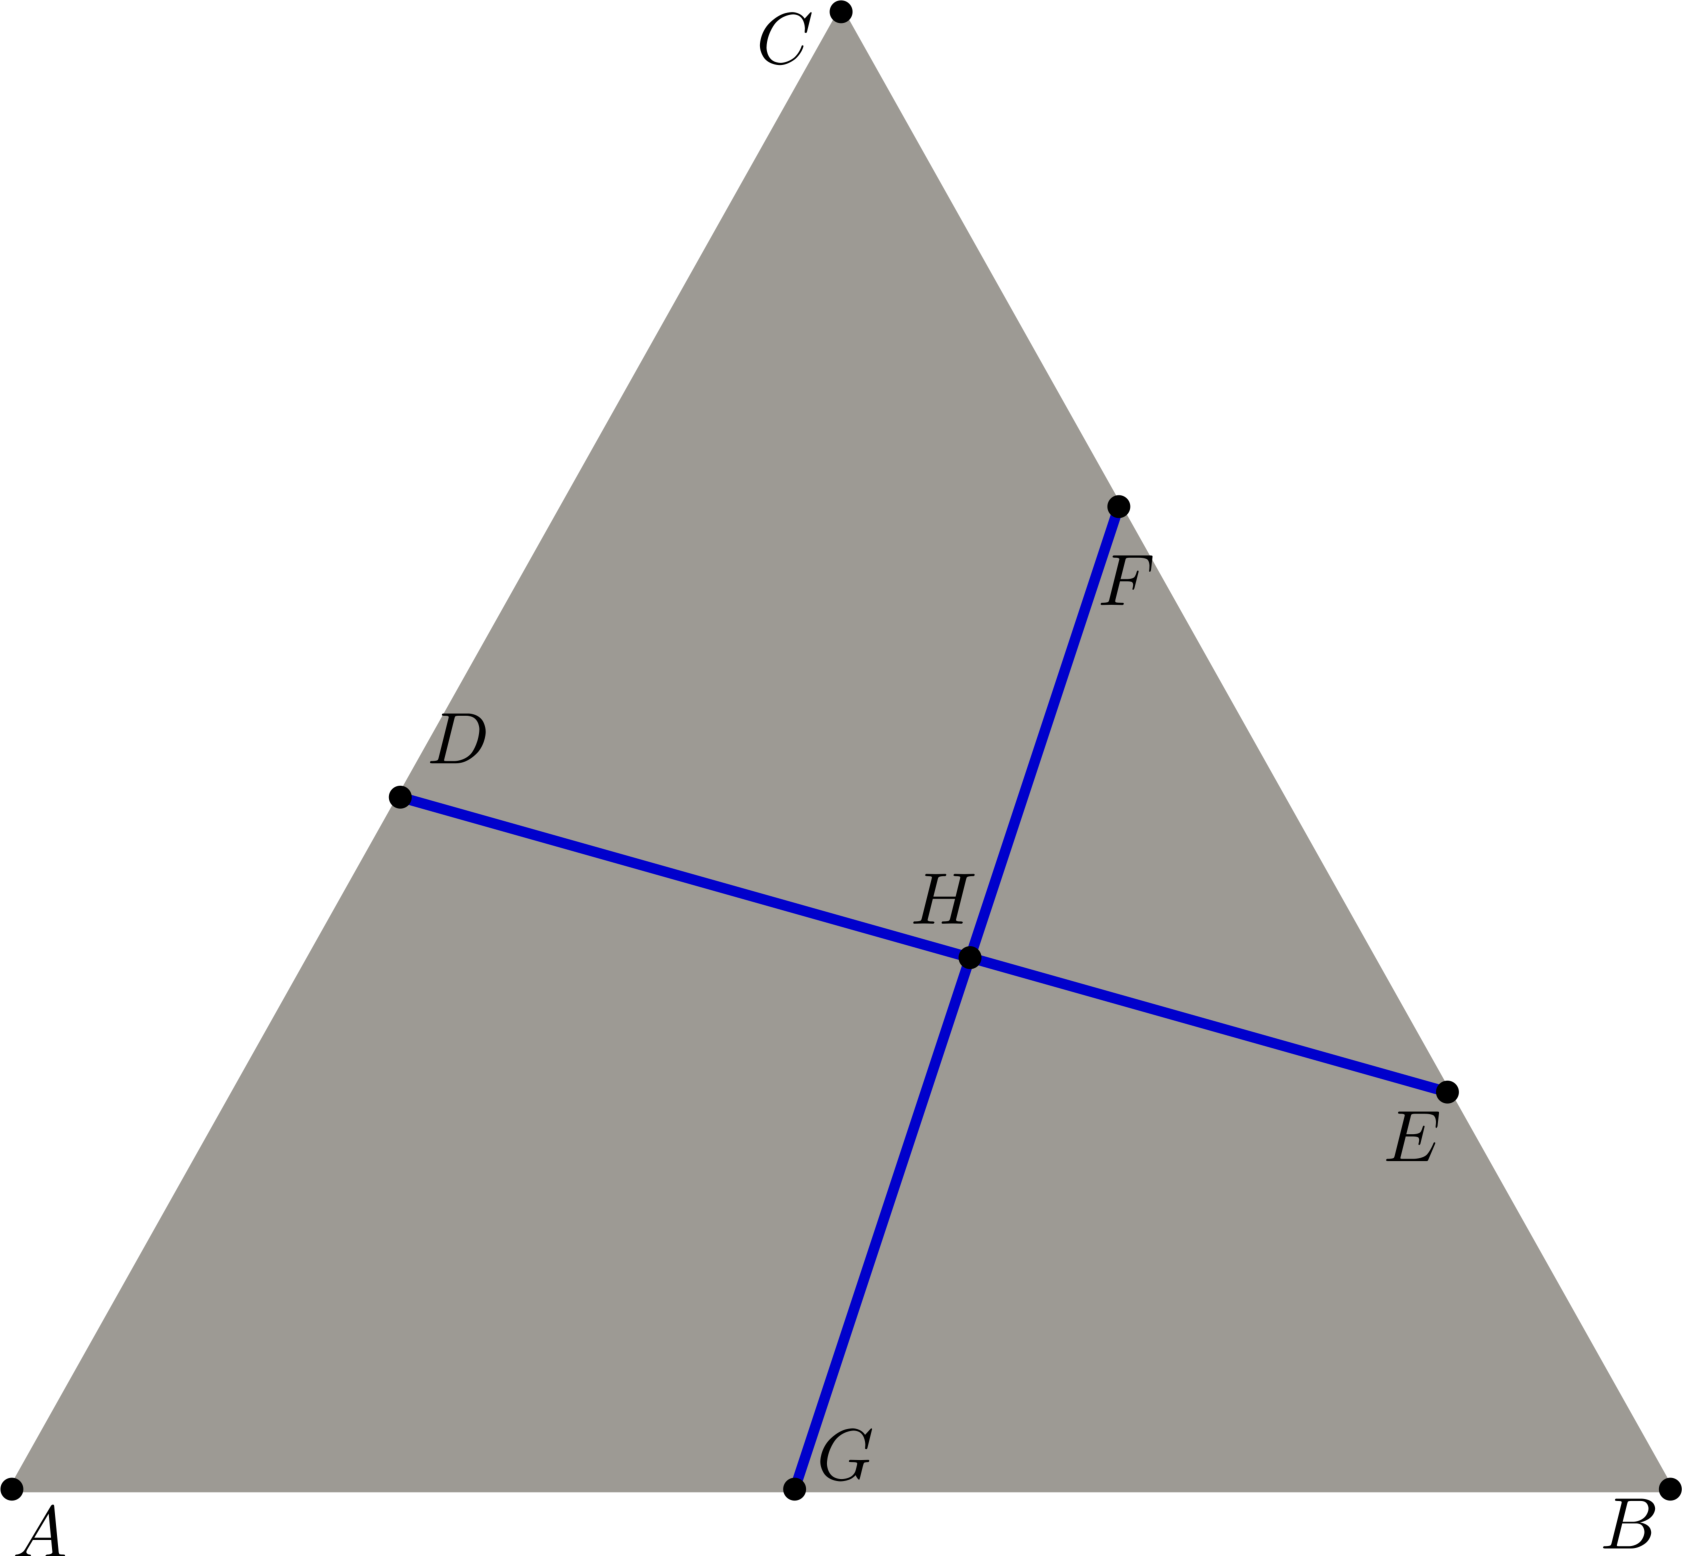
\includegraphics[width=\textwidth]{images/decoup_triangle.pdf}
    \caption{Triangle traversé par des séparatrices.}
    \label{fig:exemple_insert_pt_0}
\end{subfigure}
\hfill
\begin{subfigure}{0.45\textwidth}
    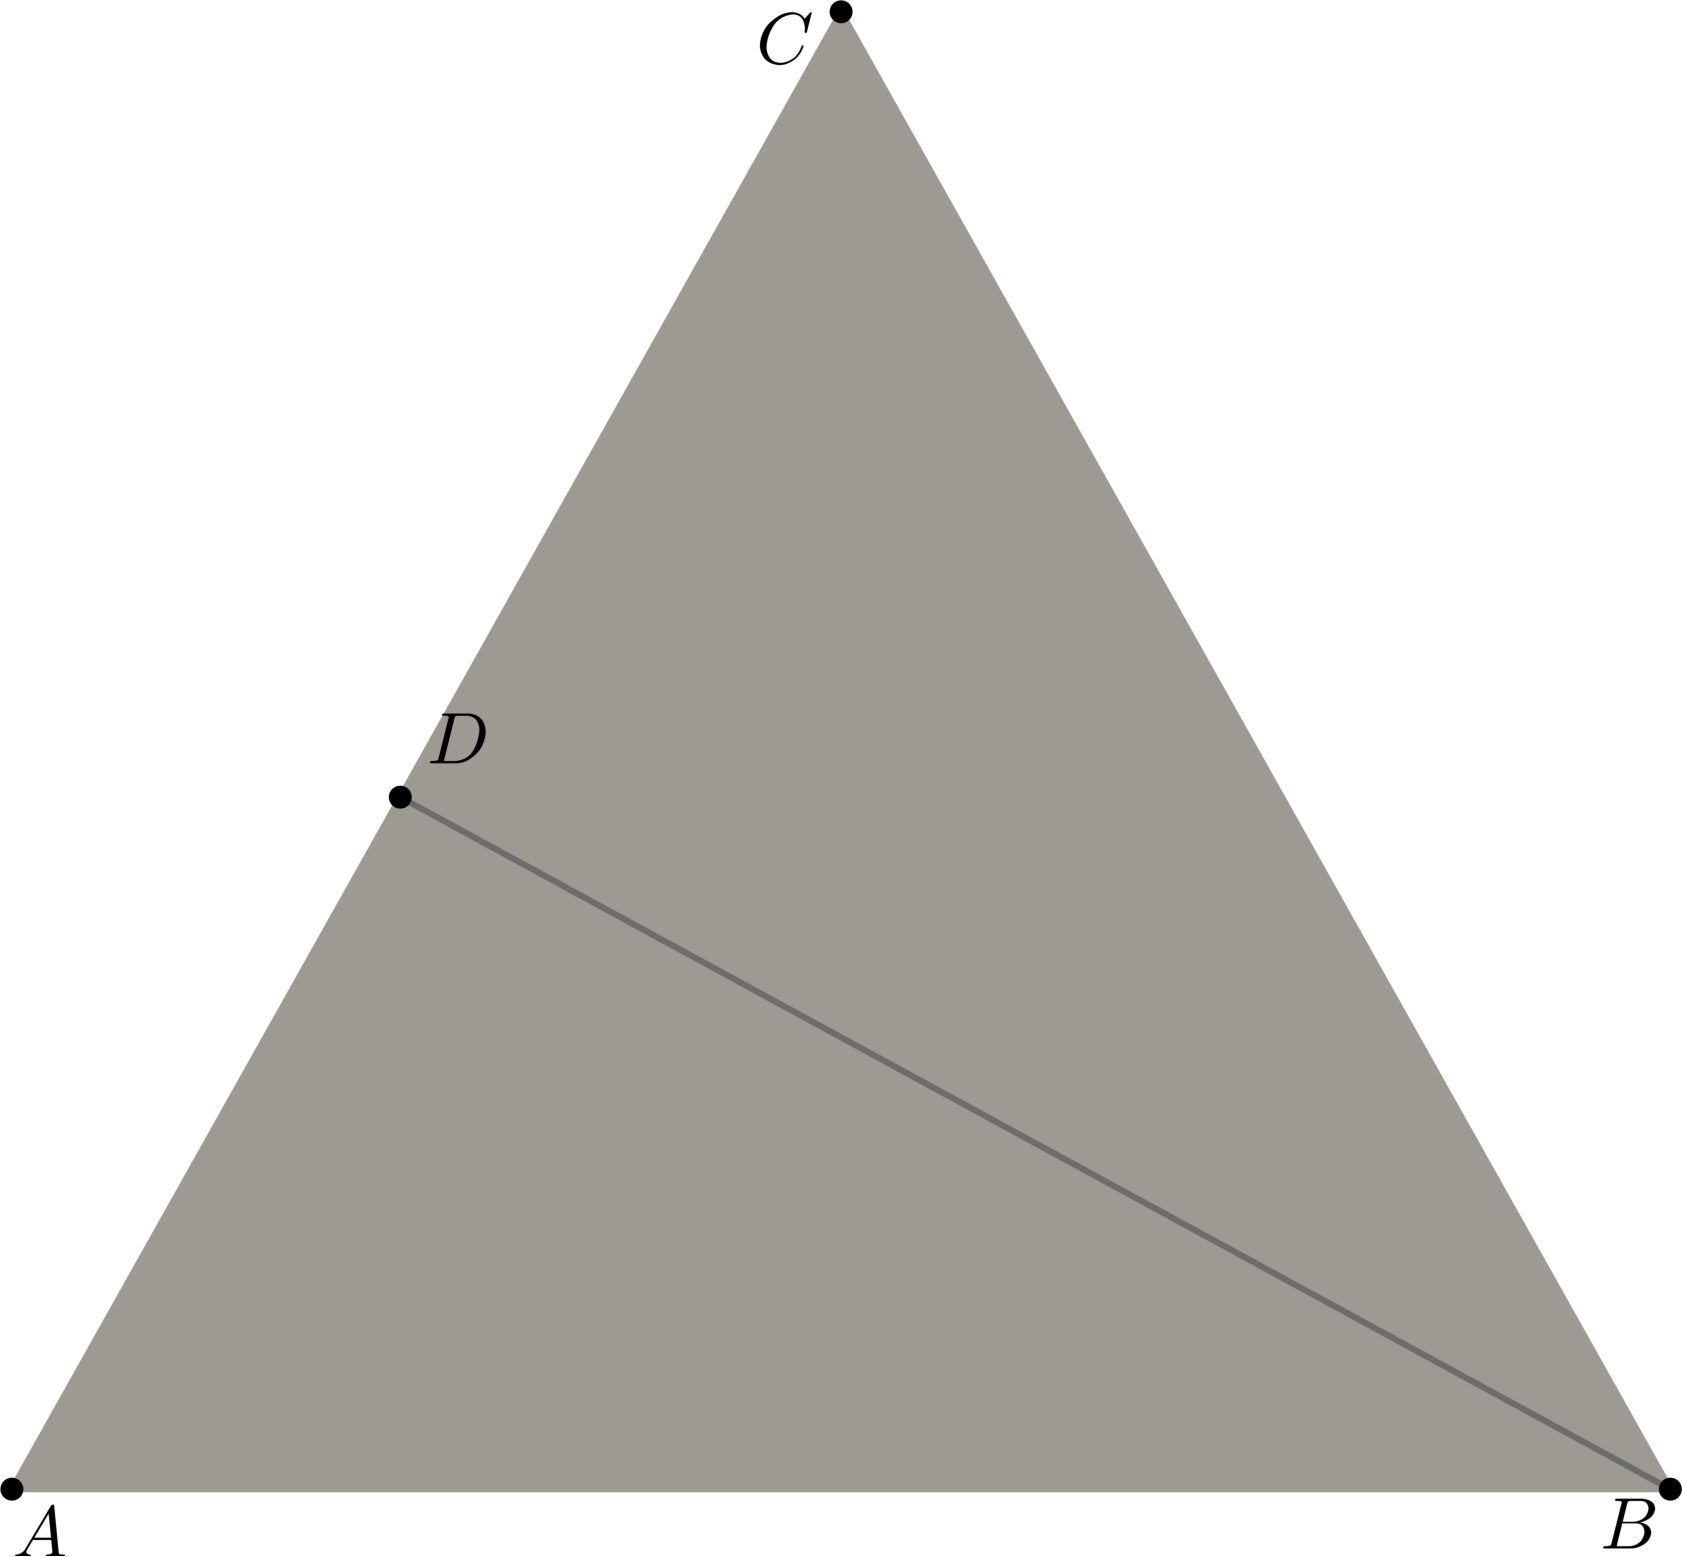
\includegraphics[width=\textwidth]{images/decoup_triangle-1.pdf}
    \caption{Insertion de $D$.}
    \label{fig:exemple_insert_pt_1}
\end{subfigure}
\\[0.1cm]
\begin{subfigure}{0.45\textwidth}
    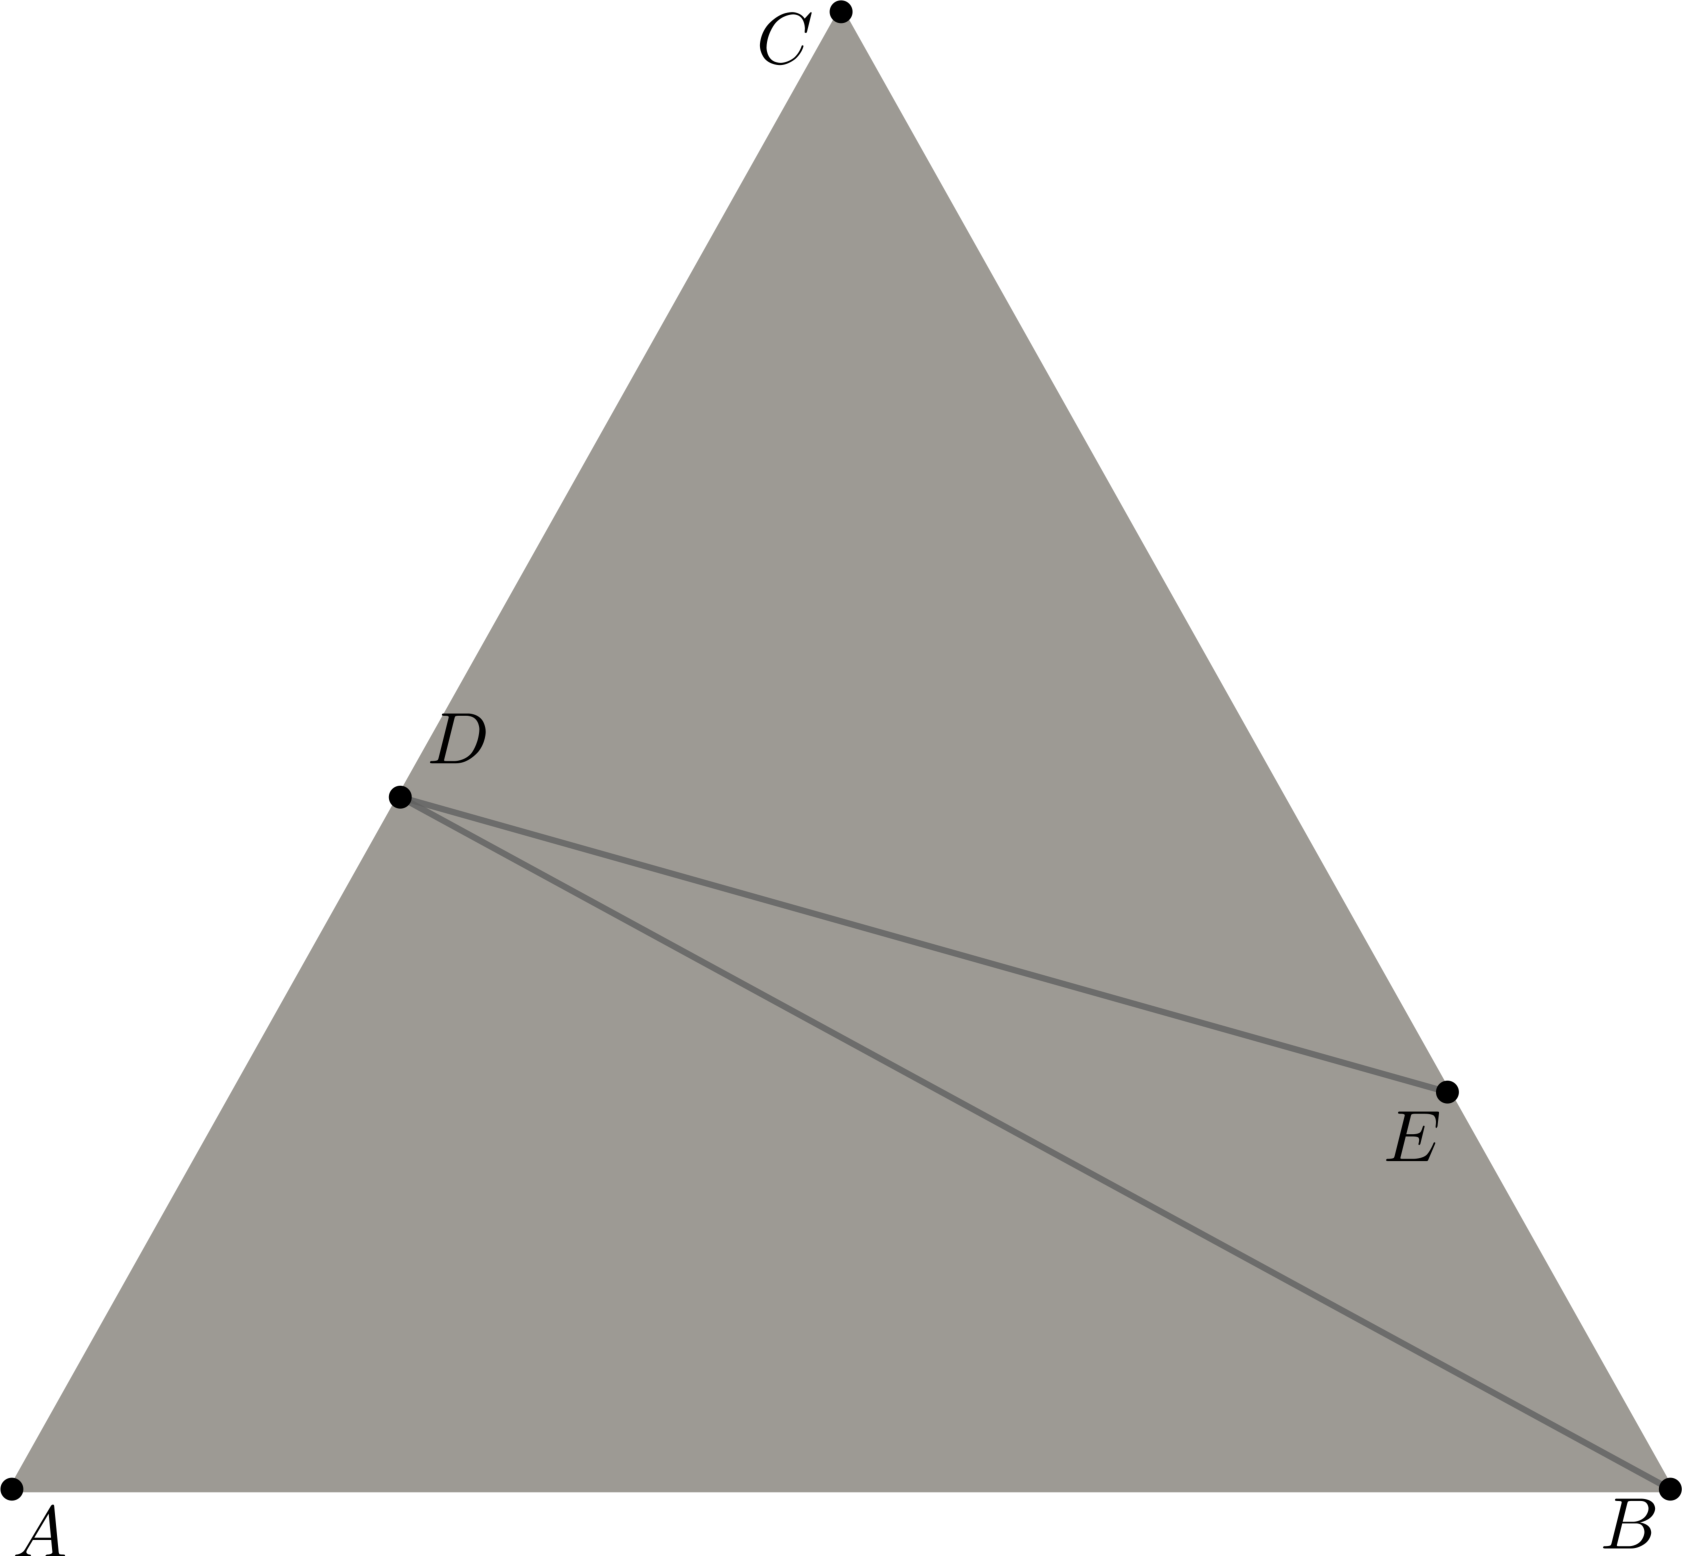
\includegraphics[width=\textwidth]{images/decoup_triangle-2.pdf}
    \caption{Insertion de $E$.}
    \label{fig:exemple_insert_pt_2}
\end{subfigure}
\hfill
\begin{subfigure}{0.45\textwidth}
    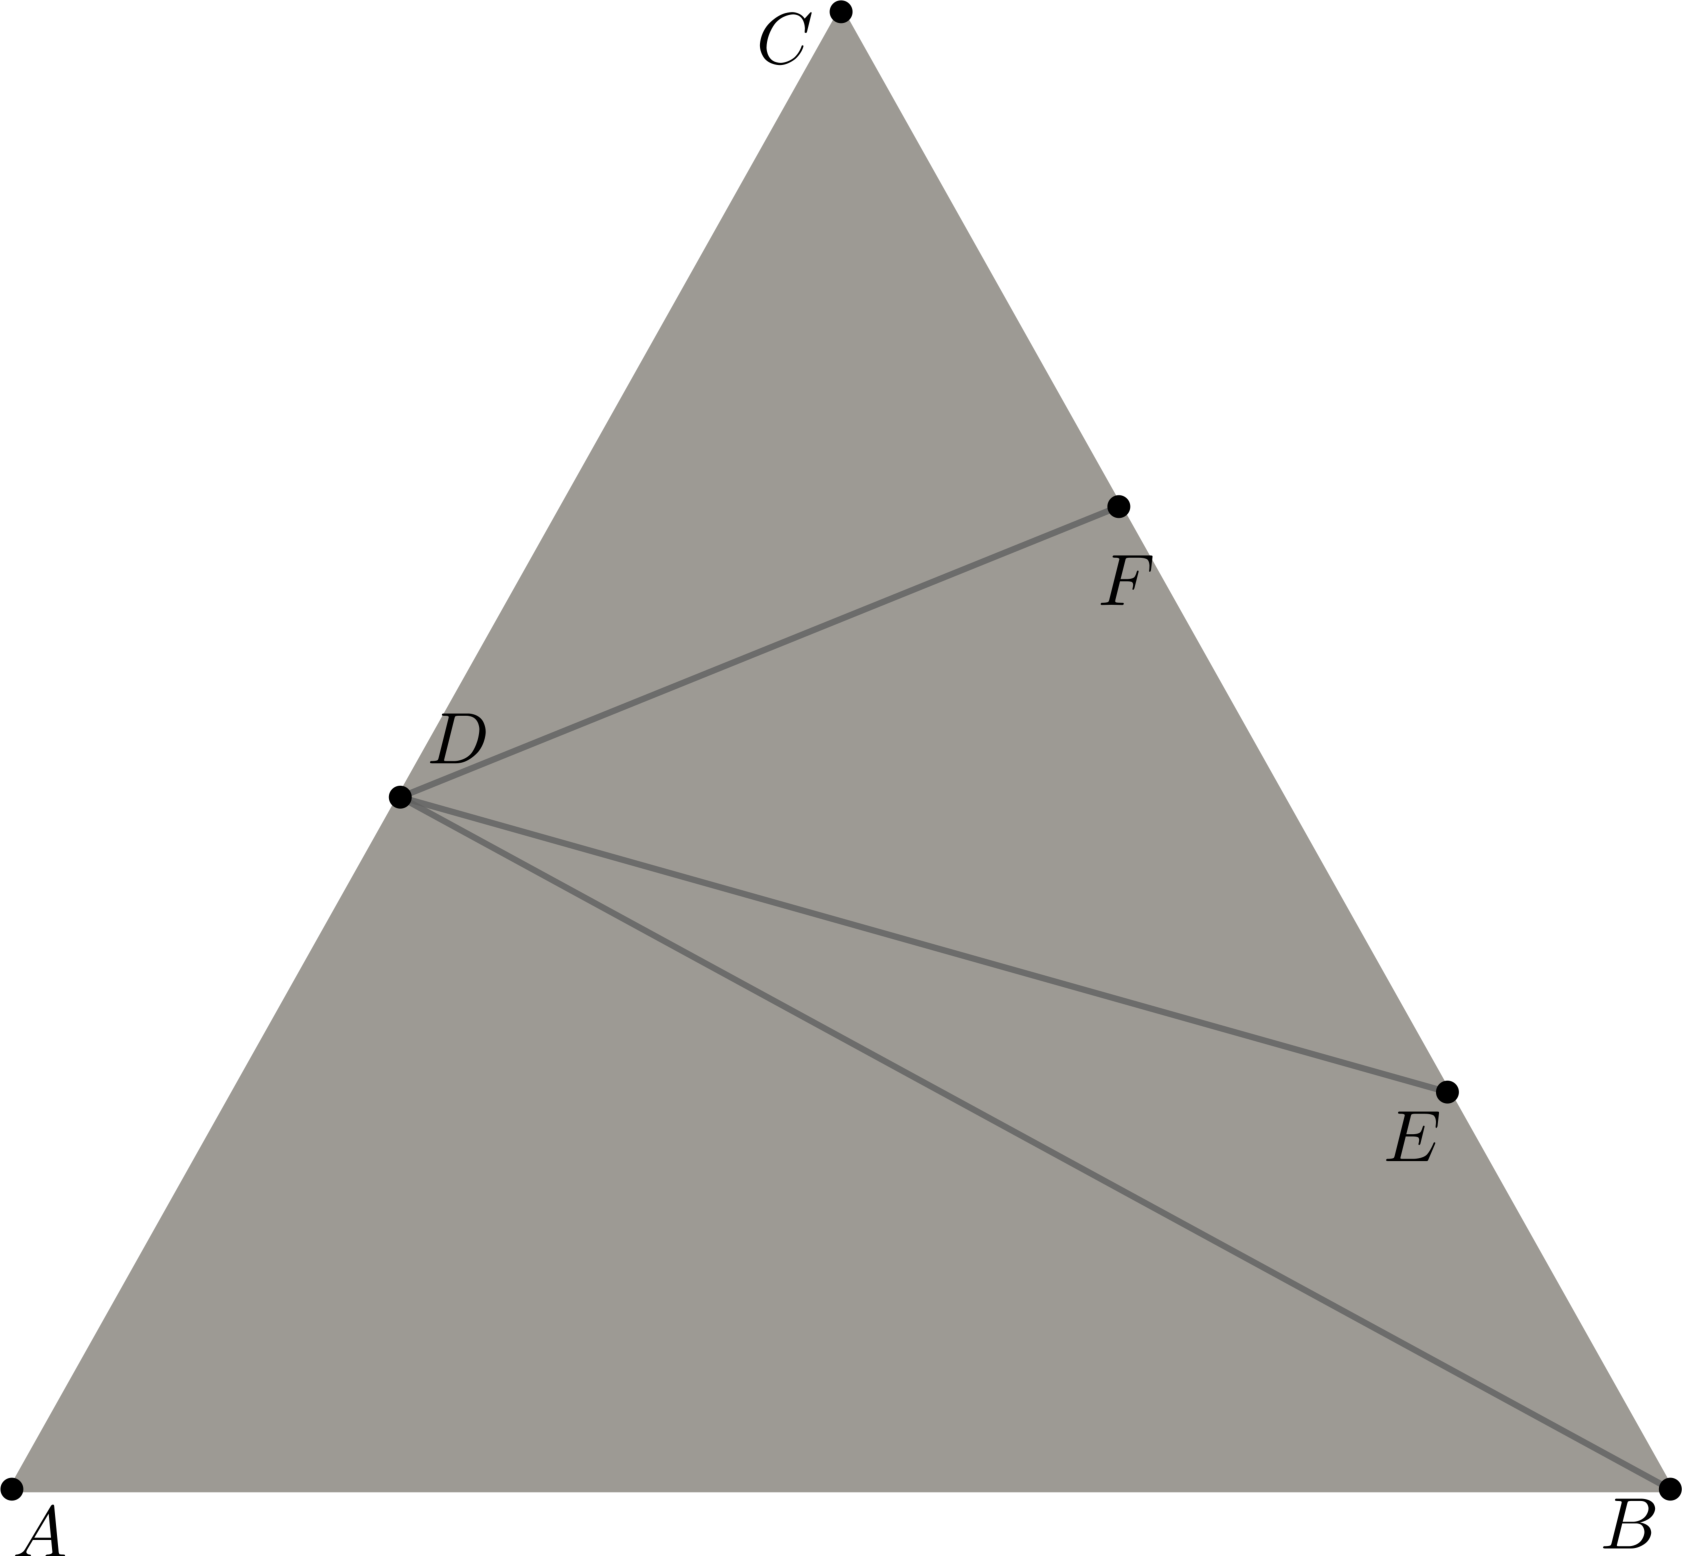
\includegraphics[width=\textwidth]{images/decoup_triangle-3.pdf}
    \caption{Insertion de $F$.}
    \label{fig:exemple_insert_pt_3}
\end{subfigure}
\\[0.1cm]
\begin{subfigure}{0.45\textwidth}
    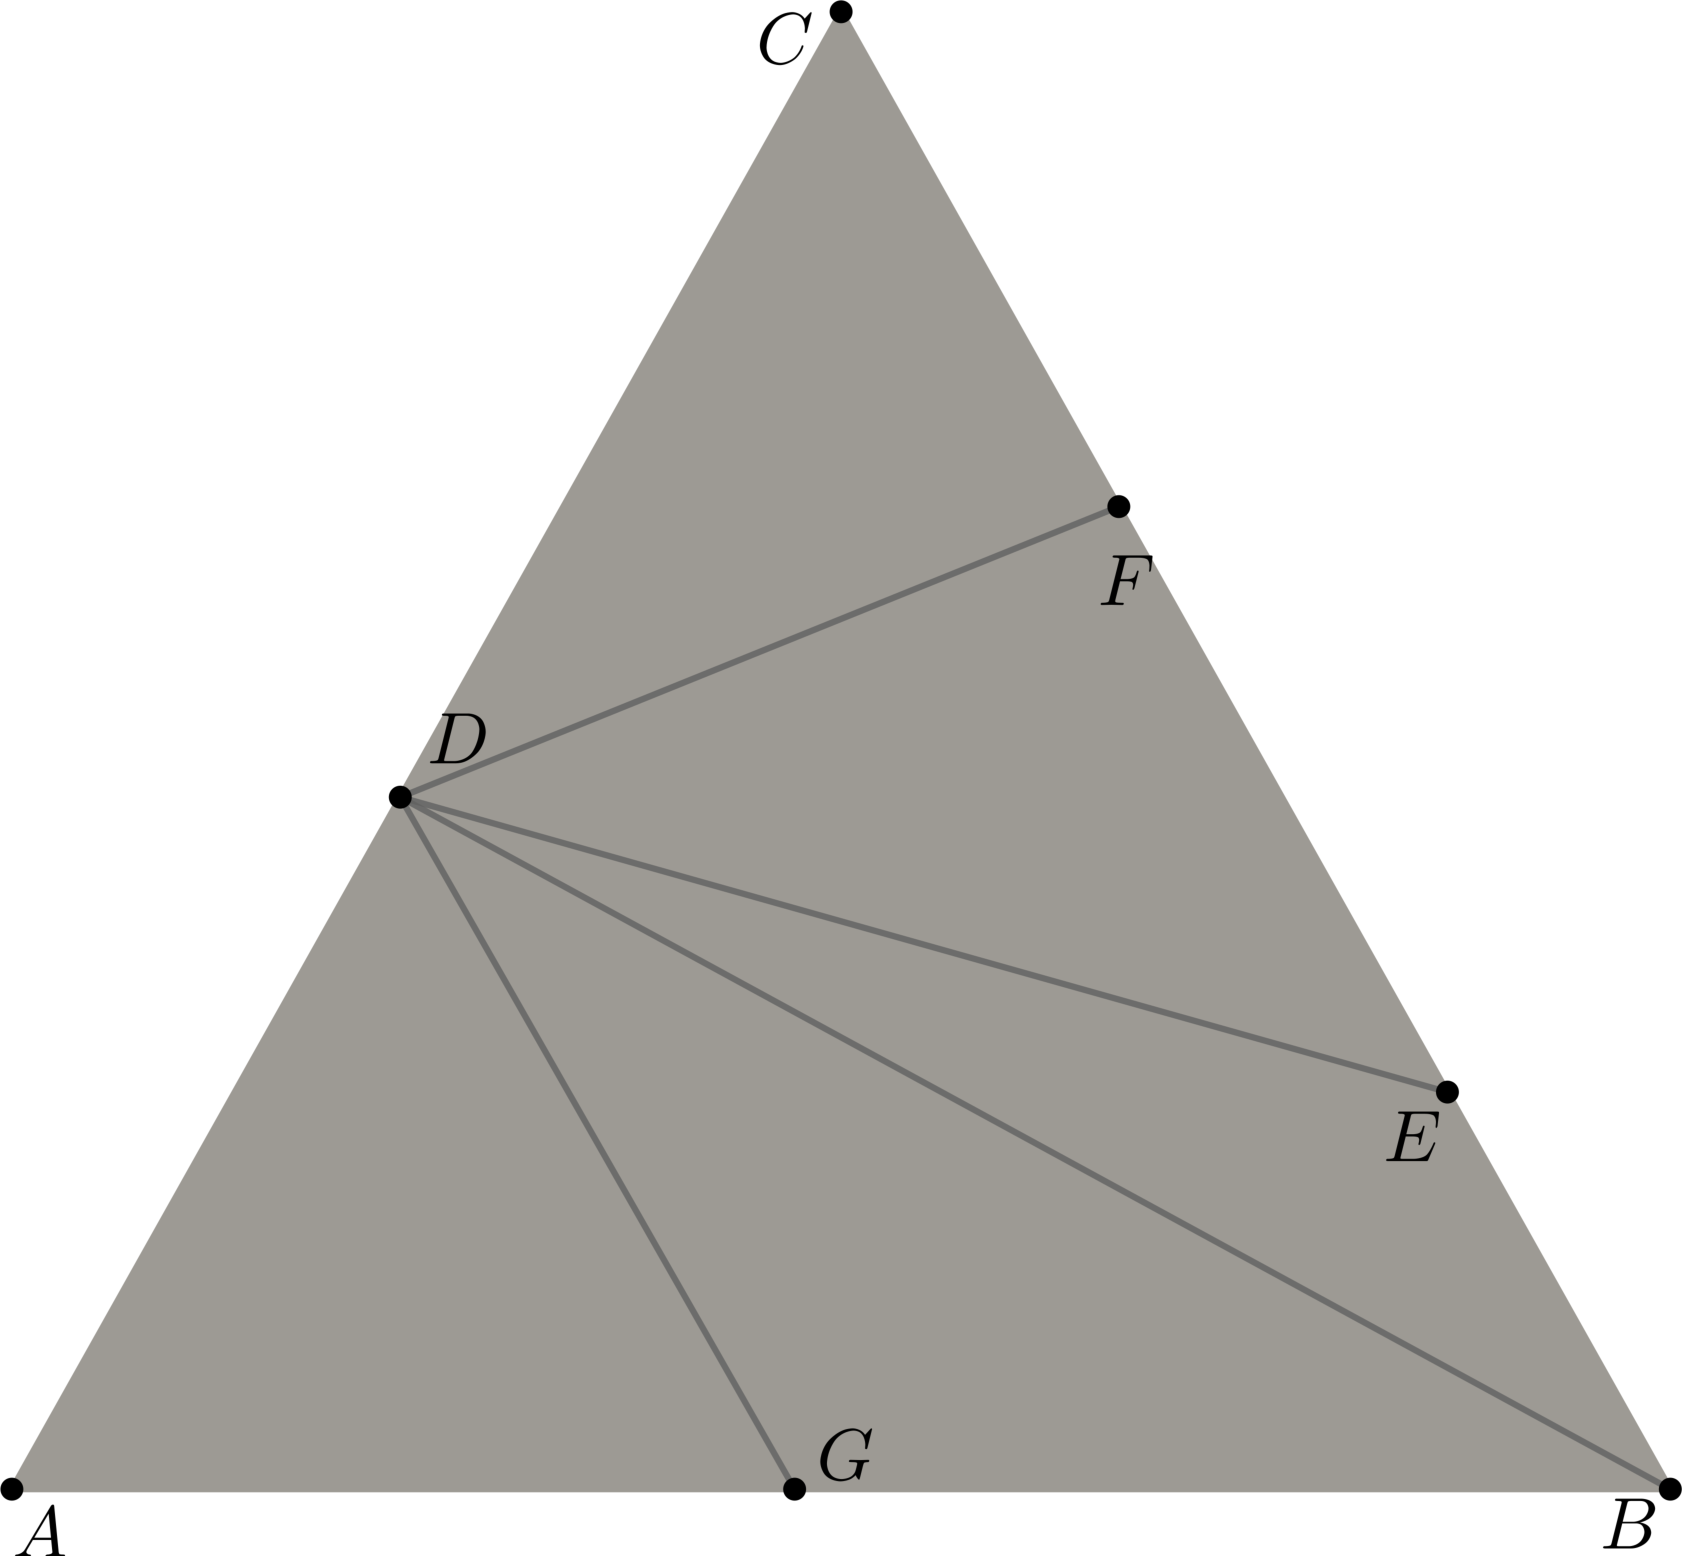
\includegraphics[width=\textwidth]{images/decoup_triangle-4.pdf}
    \caption{Insertion de $G$.}
    \label{fig:exemple_insert_pt_4}
\end{subfigure}
\hfill
\begin{subfigure}{0.45\textwidth}
    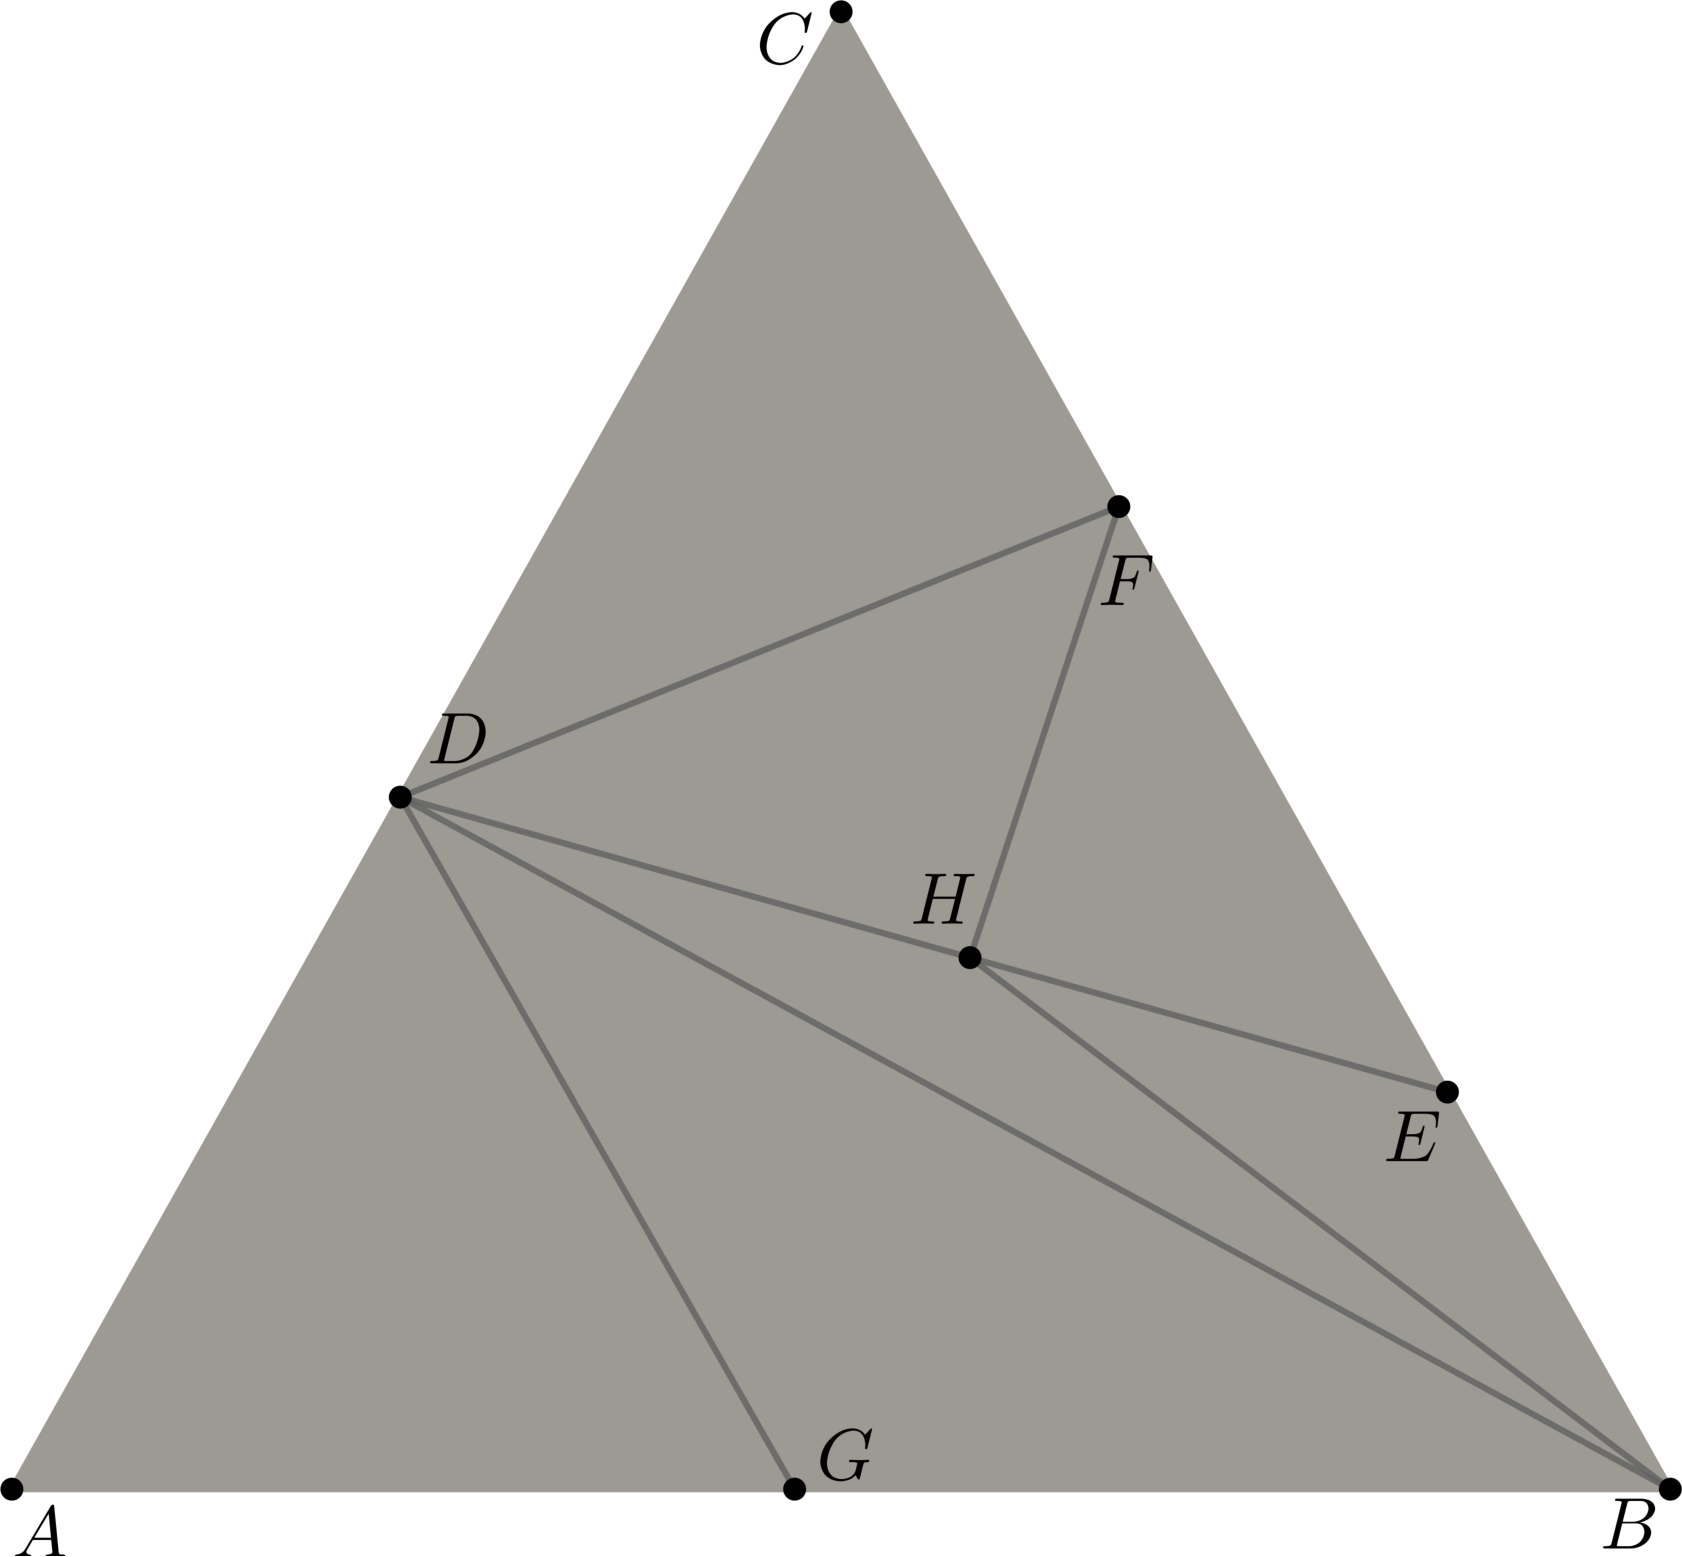
\includegraphics[width=\textwidth]{images/decoup_triangle-5.pdf}
    \caption{Insertion de $H$.}
    \label{fig:exemple_insert_pt_5}
\end{subfigure}
\caption{Adaptation locale du triangle en fonction des points de passage des séparatrices.}
\label{fig:exemple_insert_pt}
\end{figure}

Sur la figure \ref{fig:exemple_insert_pt}, nous avons quatre segments de séparatrices à considérer ($DH$, $HE$, $HG$, $FH$). Nous procédons donc à l'insertion séquentielle des points $D$, $E$, $F$, $G$, $H$ (l'ordre d'insertion est sans importance). On se retrouve alors avec un raffinement local contenant tous les points nécessaires à la suite du processus. Le raffinement ainsi produit ne contient pas en général dans la liste de ses arêtes les segments des séparatrices. La suite du processus consistera à recenser les segments des séparatrices qui n'ont pas été générés suite à l'insertion des points, puis à procéder à des ajustements locaux pour garantir leurs présences dans le raffinement effectué. Plus précisément, nous effectuerons des retournements d'arêtes en nous inspirant de la méthode de génération de maillages de type Voronoi, telle qu'exposée dans \cite{georgegeneration}: soit $T_{mesh}$ le maillage local correspondant au raffinement précédemment construit. Soit $AB$ un segment non présente dans $T_{mesh}$ et $T_{AB}$ l'ensemble des éléments de $T_{mesh}$ dont une arête est coupée par $AB$. Si le premier triangle de $T_{AB}$ (contenant $A$ comme sommet) et le second triangle de cet ensemble (le voisin d'arête commune, oposée à $A$) forment un polygone convexe, on peut appliquer le retournement d'arête. On supprime ainsi l'arête commune et on génère une nouvelle arête sans intersection avec $AB$. Ce processus est similaire pour le dernier élément (ayant $B$ comme sommet) et l'avant-dernier. Cela permet d'avancer sans que l'arête nouvellement créée ne croise $AB$. En itérant ce processus, le polygone $T_{AB}$ est remaillé et l'arête $AB$ est désormais présente comme une arête d'un triangle (voir figure \ref{fig:retournement_arete_george}). Une formalistaion de ce procédé est illustré par l'algorithme \ref{alg:retournement_arete}.

\begin{figure}[h!]
\centering
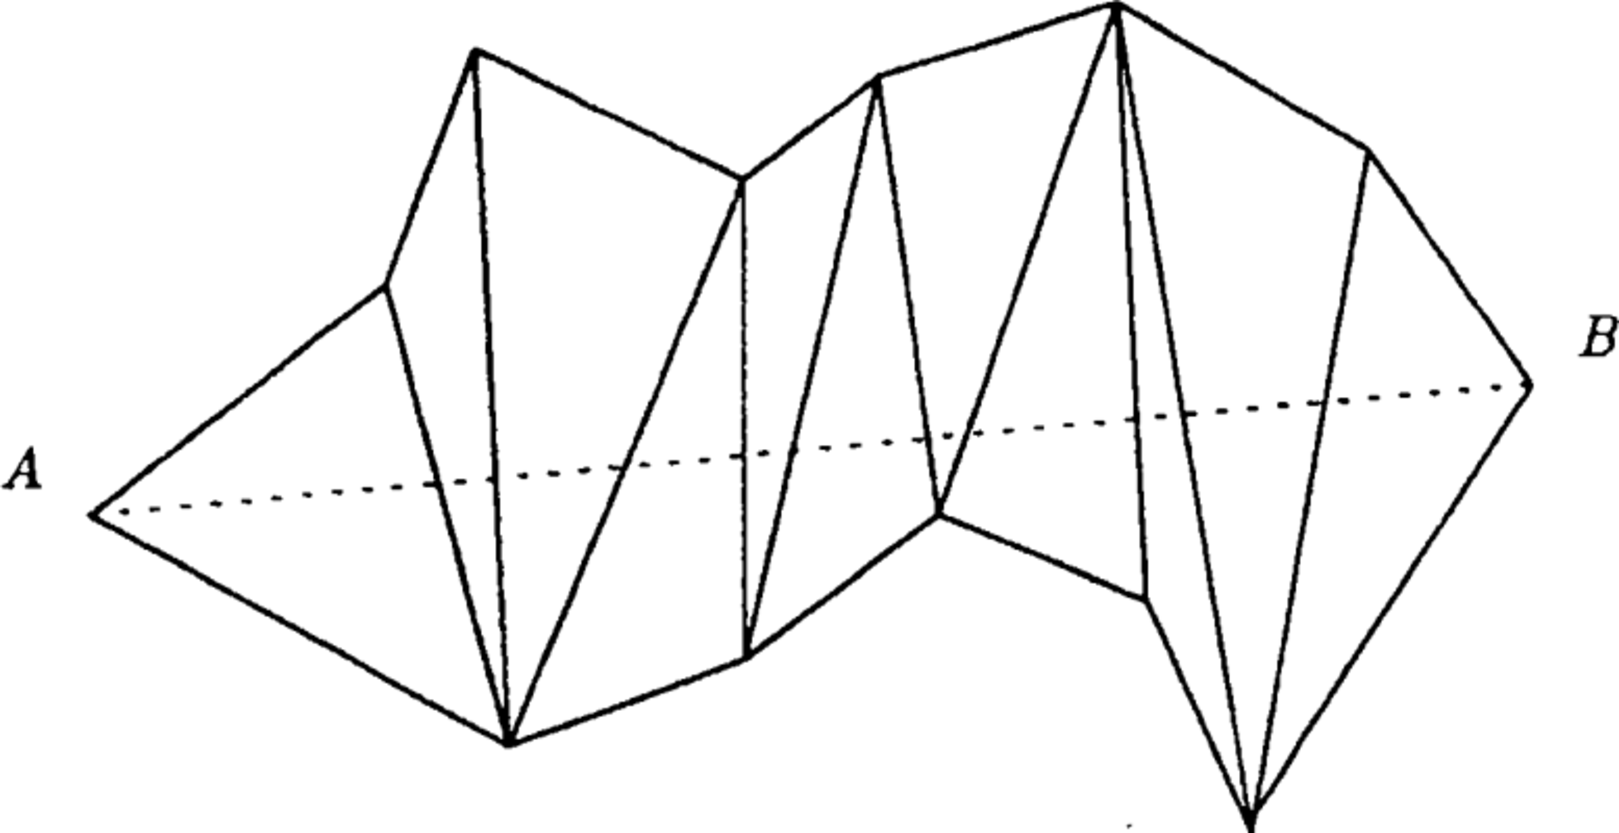
\includegraphics[scale=0.275]{images/retourn_arete_george-1.pdf}\hfill
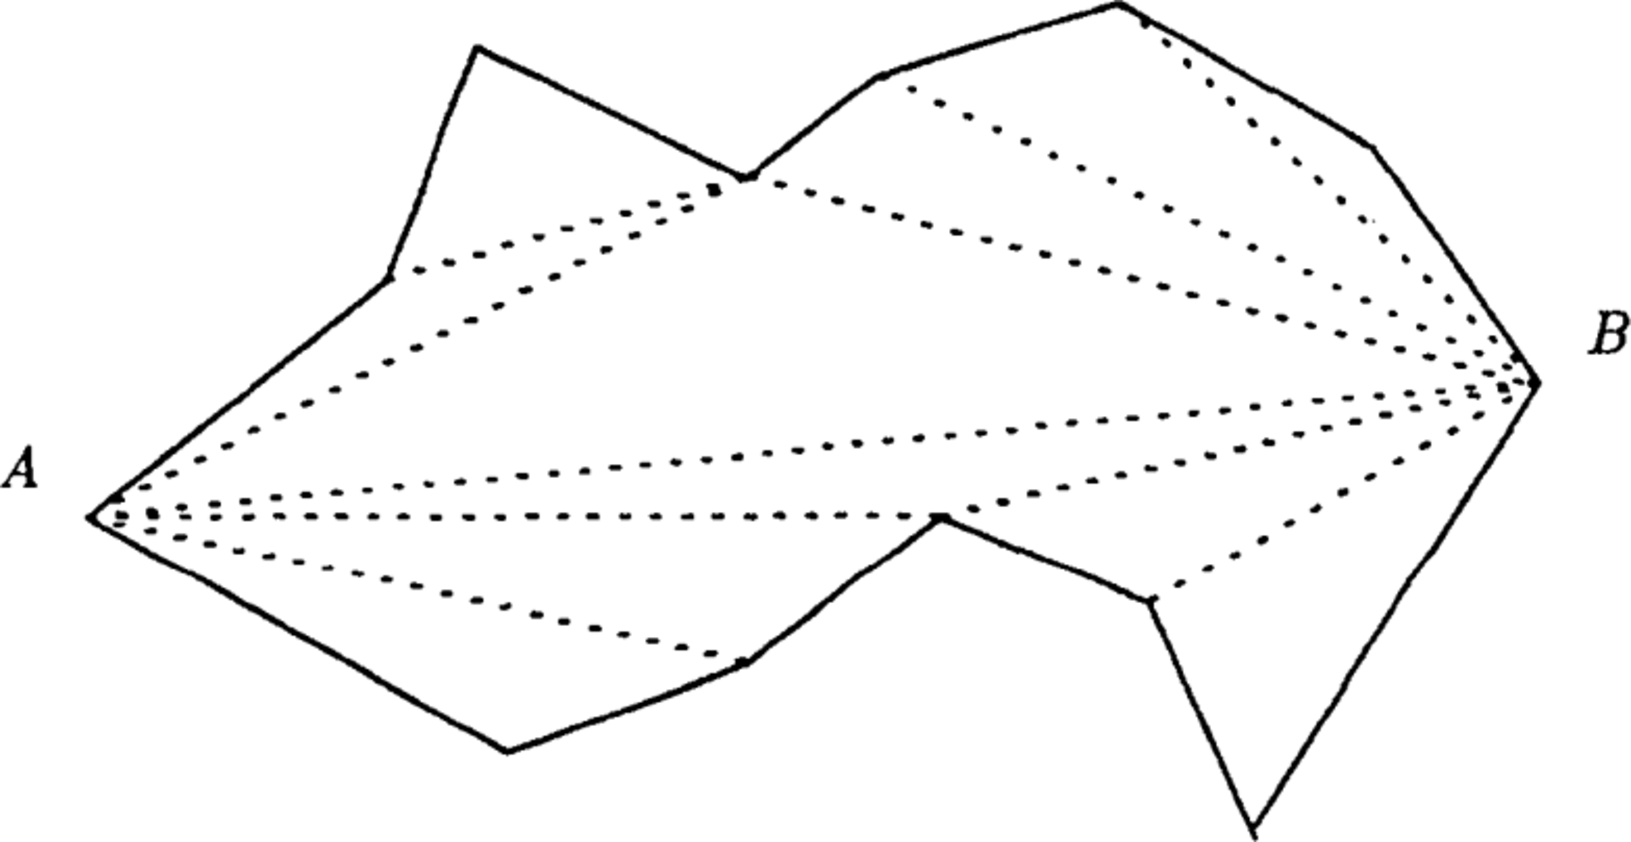
\includegraphics[scale=0.275]{images/retourn_arete_george-2.pdf}
\caption{Forçage par retournement. Source: \cite{georgegeneration}.}
\label{fig:retournement_arete_george}
\end{figure}

\vspace{0.5cm}
\RestyleAlgo{ruled}
\begin{algorithm}[h!]
\renewcommand{\algorithmcfname}{Algorithme}%
\SetAlgoLined
\Entree{Triangle $T$, Liste des séparatrices}
\Sortie{Maillage local $T_{mesh}$ de $T$ contenant dans sa liste d'arêtes les segments des séparatrices inclus dans $T$}
\vspace{0.2cm}
1.\quad Initialisation $T_{mesh}=T$\\[0.2cm]
2.\quad Insertion des points aux extrémités des segments comme illustré sur la figure \ref{fig:insert_pt}\\[0.2cm]
\PourTous{segments $AB$ n'appartenant pas à la liste des arêtes de $T_{mesh}$}{
\vspace{0.2cm}
3.\quad Construire $T_{AB}$\\[0.2cm]
\Repeter{ce que $Card(T_{AB})=2$}{
\vspace{0.2cm}
\Repeter{ce que le retournement d'arête marche}{
\vspace{0.2cm}
4.\quad Itérer sur les arêtes de $T_{AB}$ interscectant $AB$\\[0.2cm]
5.\quad Tenter le retournement d'arête
\vspace{0.2cm}
}
\vspace{0.2cm}
6.\quad Mettre à jour $T_{AB}$
\vspace{0.2cm}
}
\vspace{0.2cm}
}
\caption{Forçage des segments des séparatrices}
\label{alg:retournement_arete}
\end{algorithm}
\vspace{0.5cm}

En appliquant l'algorithme \ref{alg:retournement_arete} à l'exemple de la figure \ref{fig:exemple_insert_pt}, on observe que le segment $GH$ n'est pas inclus parmi les arêtes de $T_{mesh}$. On forme ensuite $T_{GH}$ à partir des triangles $BDG$ et $BHD$. En modifiant l'arête $DB$ en $GH$, nous constatons que le polygone $DGBH$ reste convexe, confirmant ainsi le succès du retournement d'arête. Cela nous donne les nouveaux triangles $DGH$ et $GBH$ inclus parmi les triangles de $T_{mesh}$, ainsi que l'arête $GH$ ajoutée aux arêtes de $T_{mesh}$ que nous cherchions à récupérer (voir figure \ref{fig:retournement_arete}).

\begin{figure}[h!]
\centering
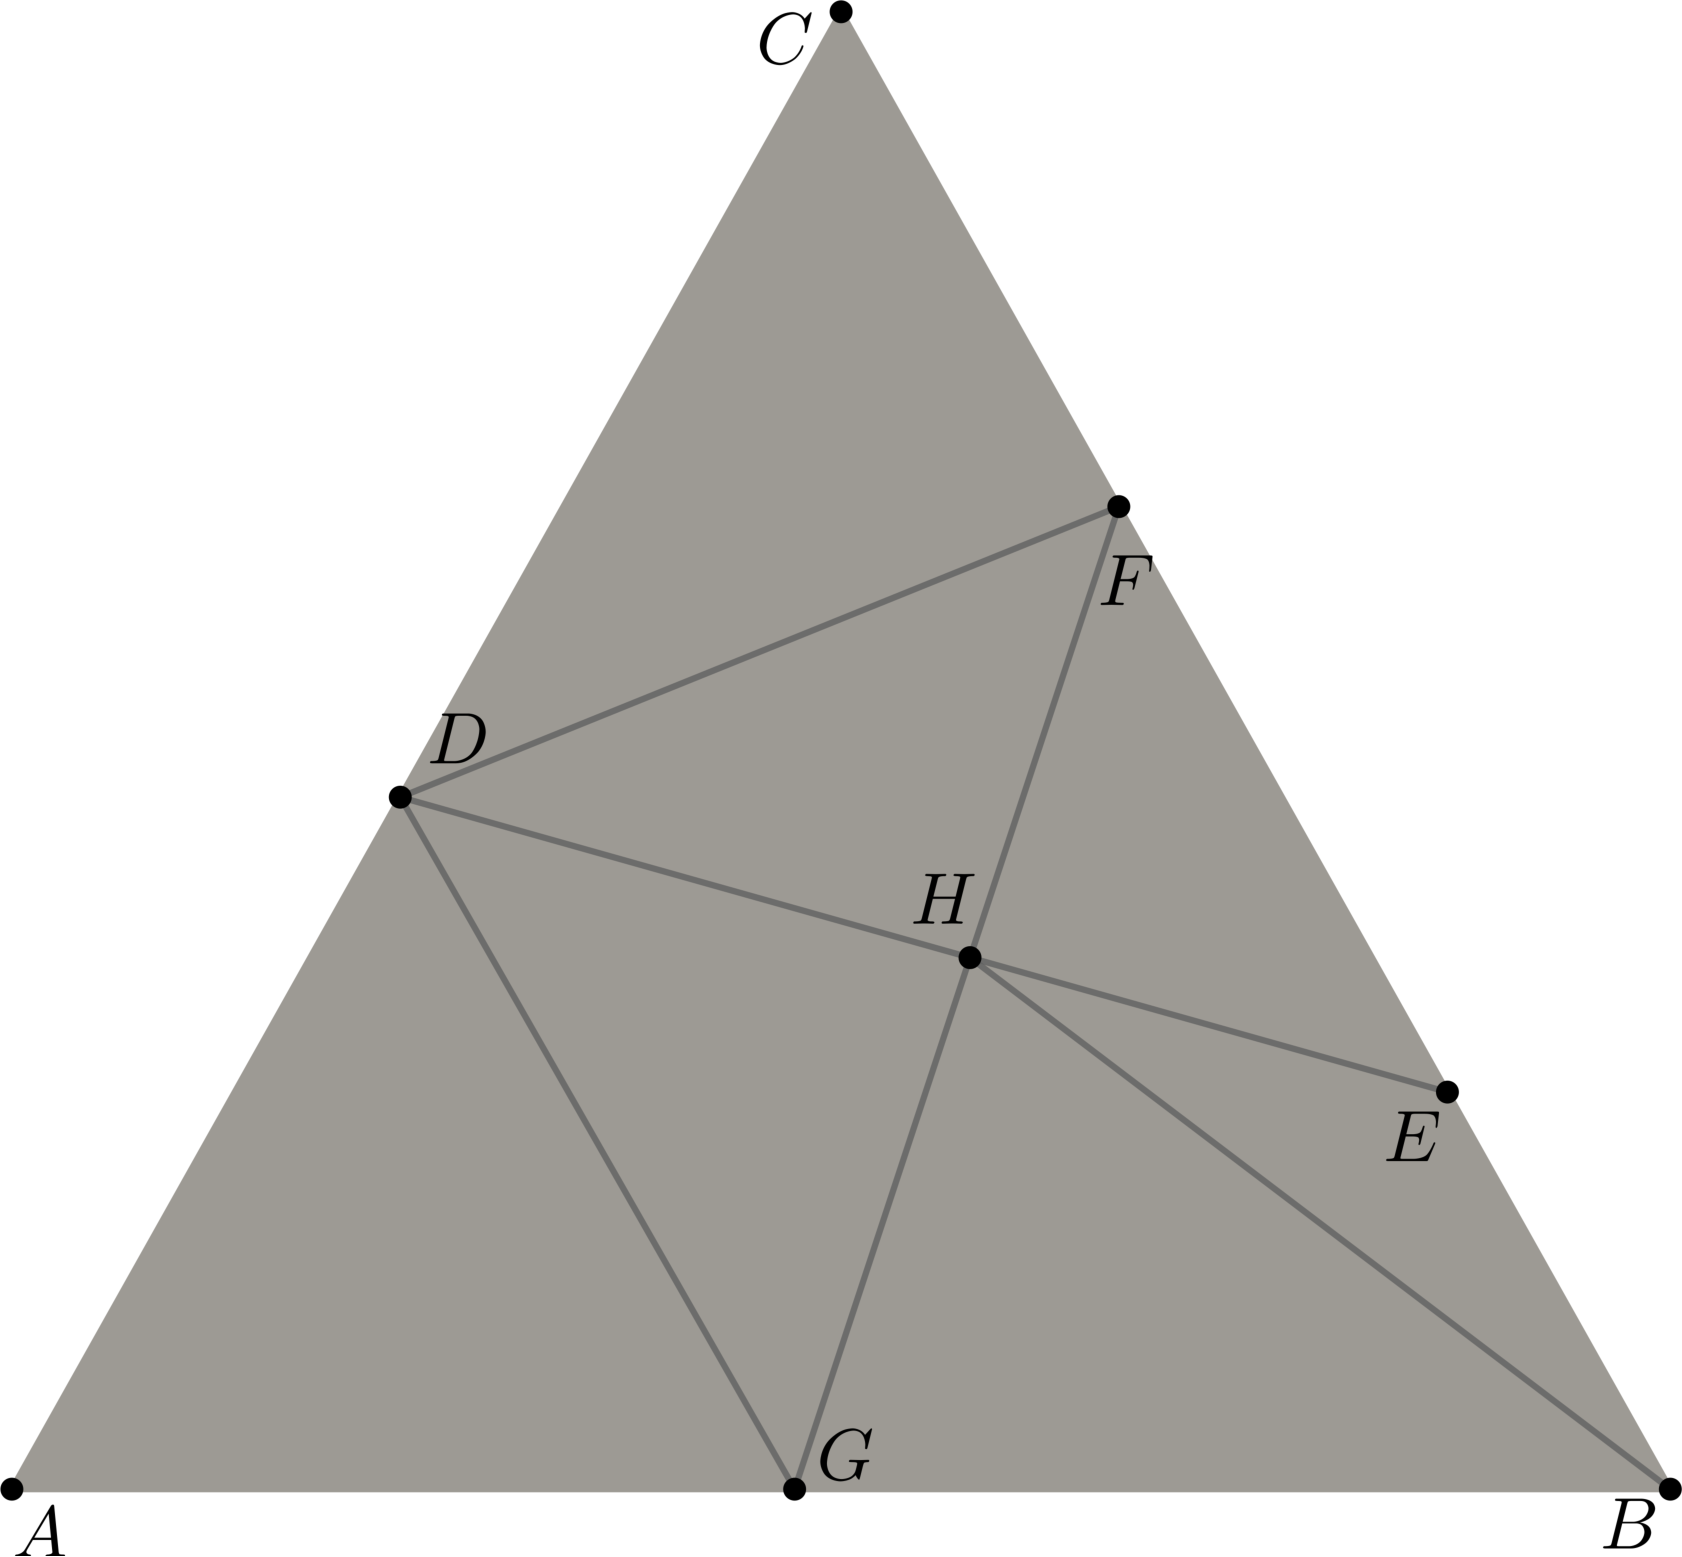
\includegraphics[scale=0.275]{images/retournement_arete-1.pdf}\hfill
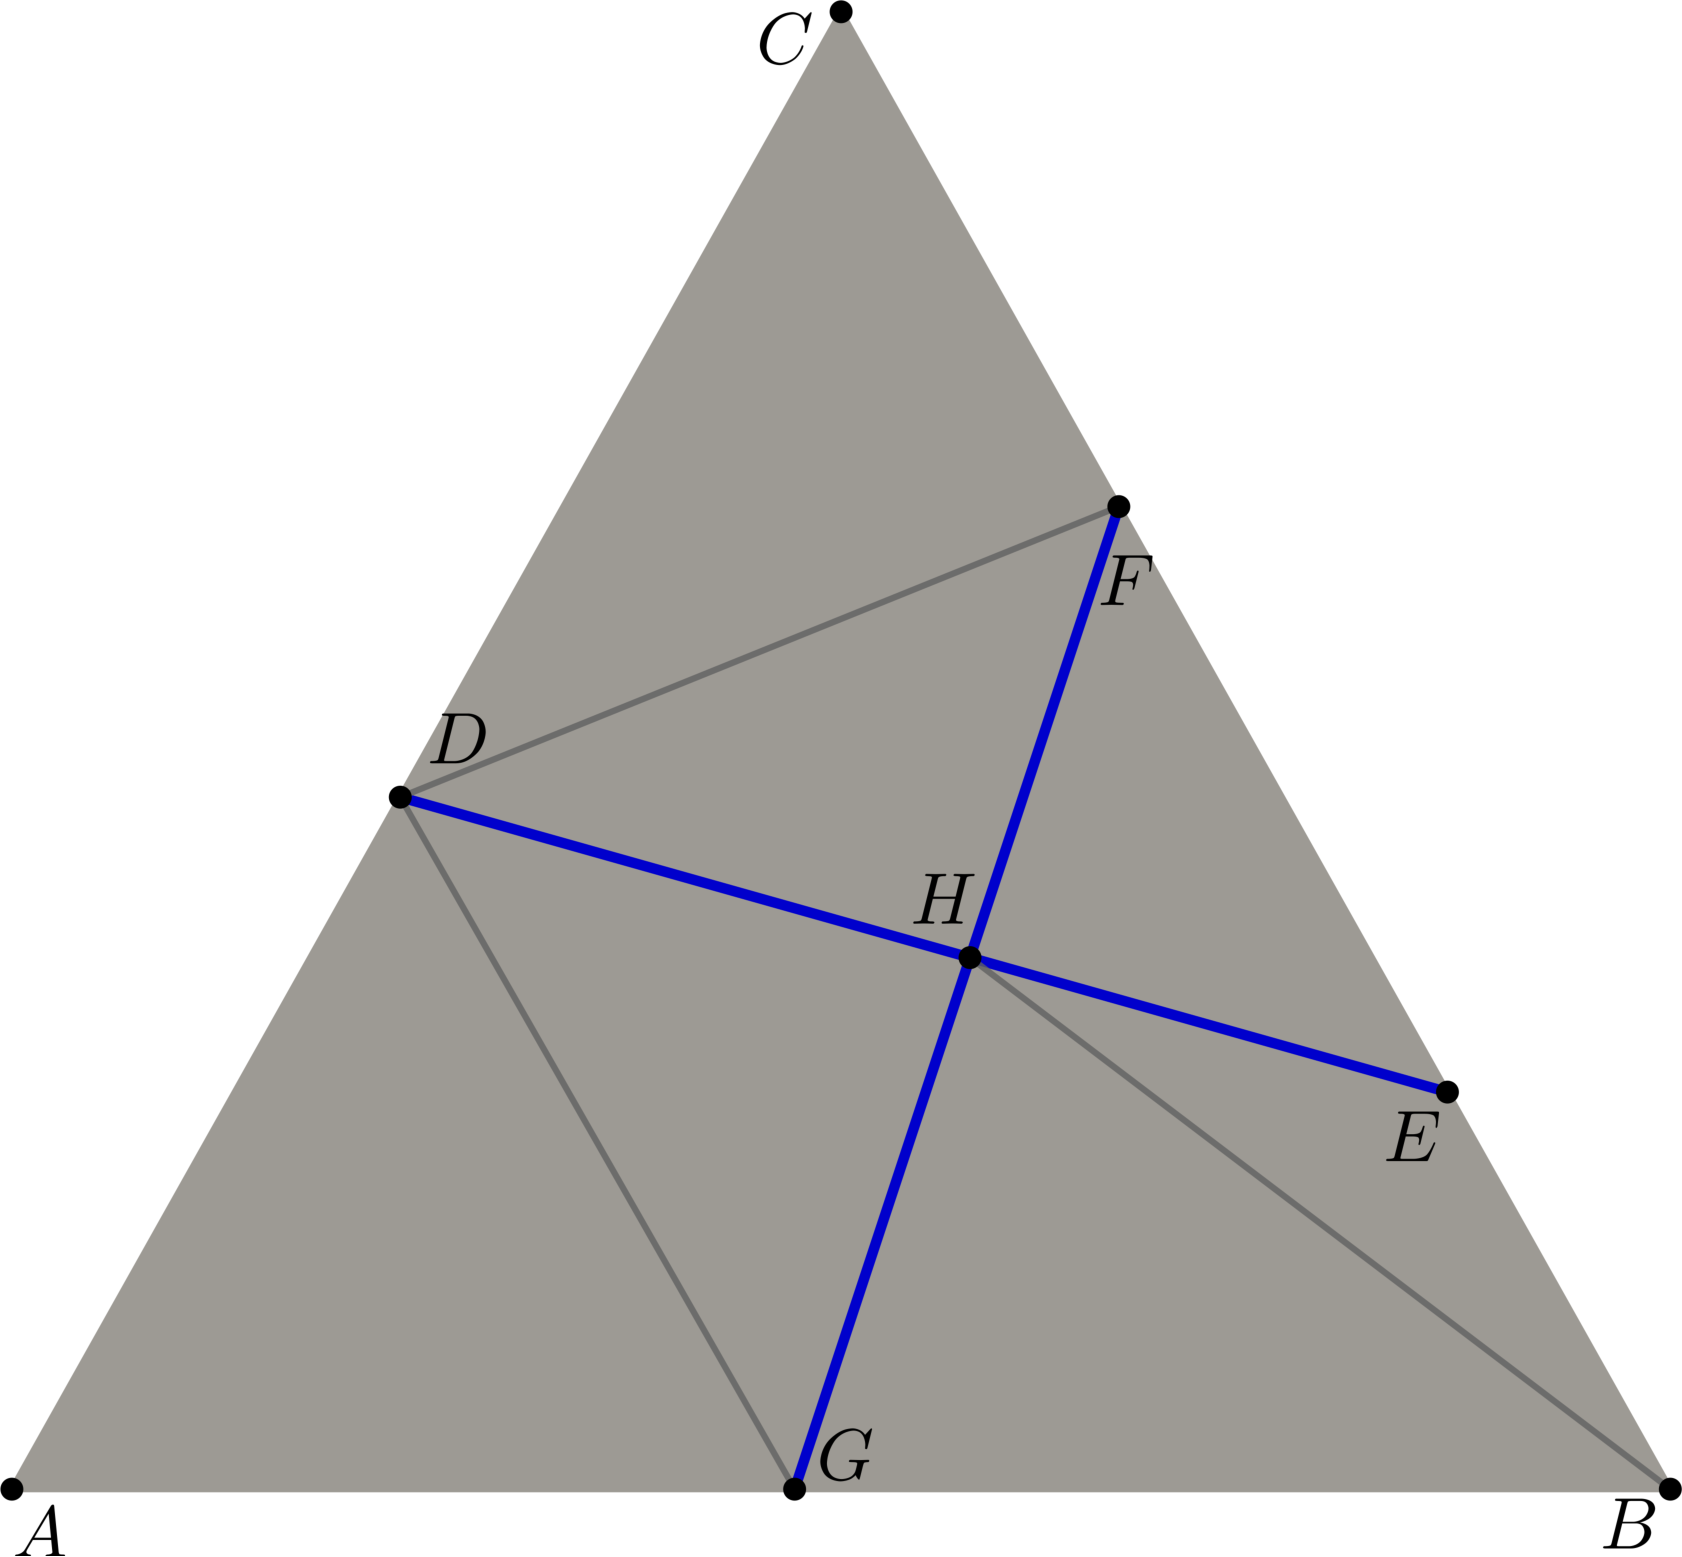
\includegraphics[scale=0.275]{images/retournement_arete-2.pdf}
\caption{Retrournement d'arête suite à l'exemple de la figure \ref{fig:exemple_insert_pt}.}
\label{fig:retournement_arete}
\end{figure}

En appliquant le processus précédemment décrit à l'exemple de la figure \ref{fig:detect_intersection}, on modifie localement chaque triangle traversé par une séparatrice ce qui nous donne un maillage global adapté au partitionnement effectué. Il ne reste plus qu'à récupérer chaque partition sous la forme d'un sous-maillage, ce qui peut être réalisé grâce à un algorithme de coloriage (voir Annexe \ref{algo_glouton}). Le résultat est illustré sur la figure \ref{fig:eclatement}.

\begin{figure}[h!]
\centering
\begin{subfigure}{0.49\textwidth}
    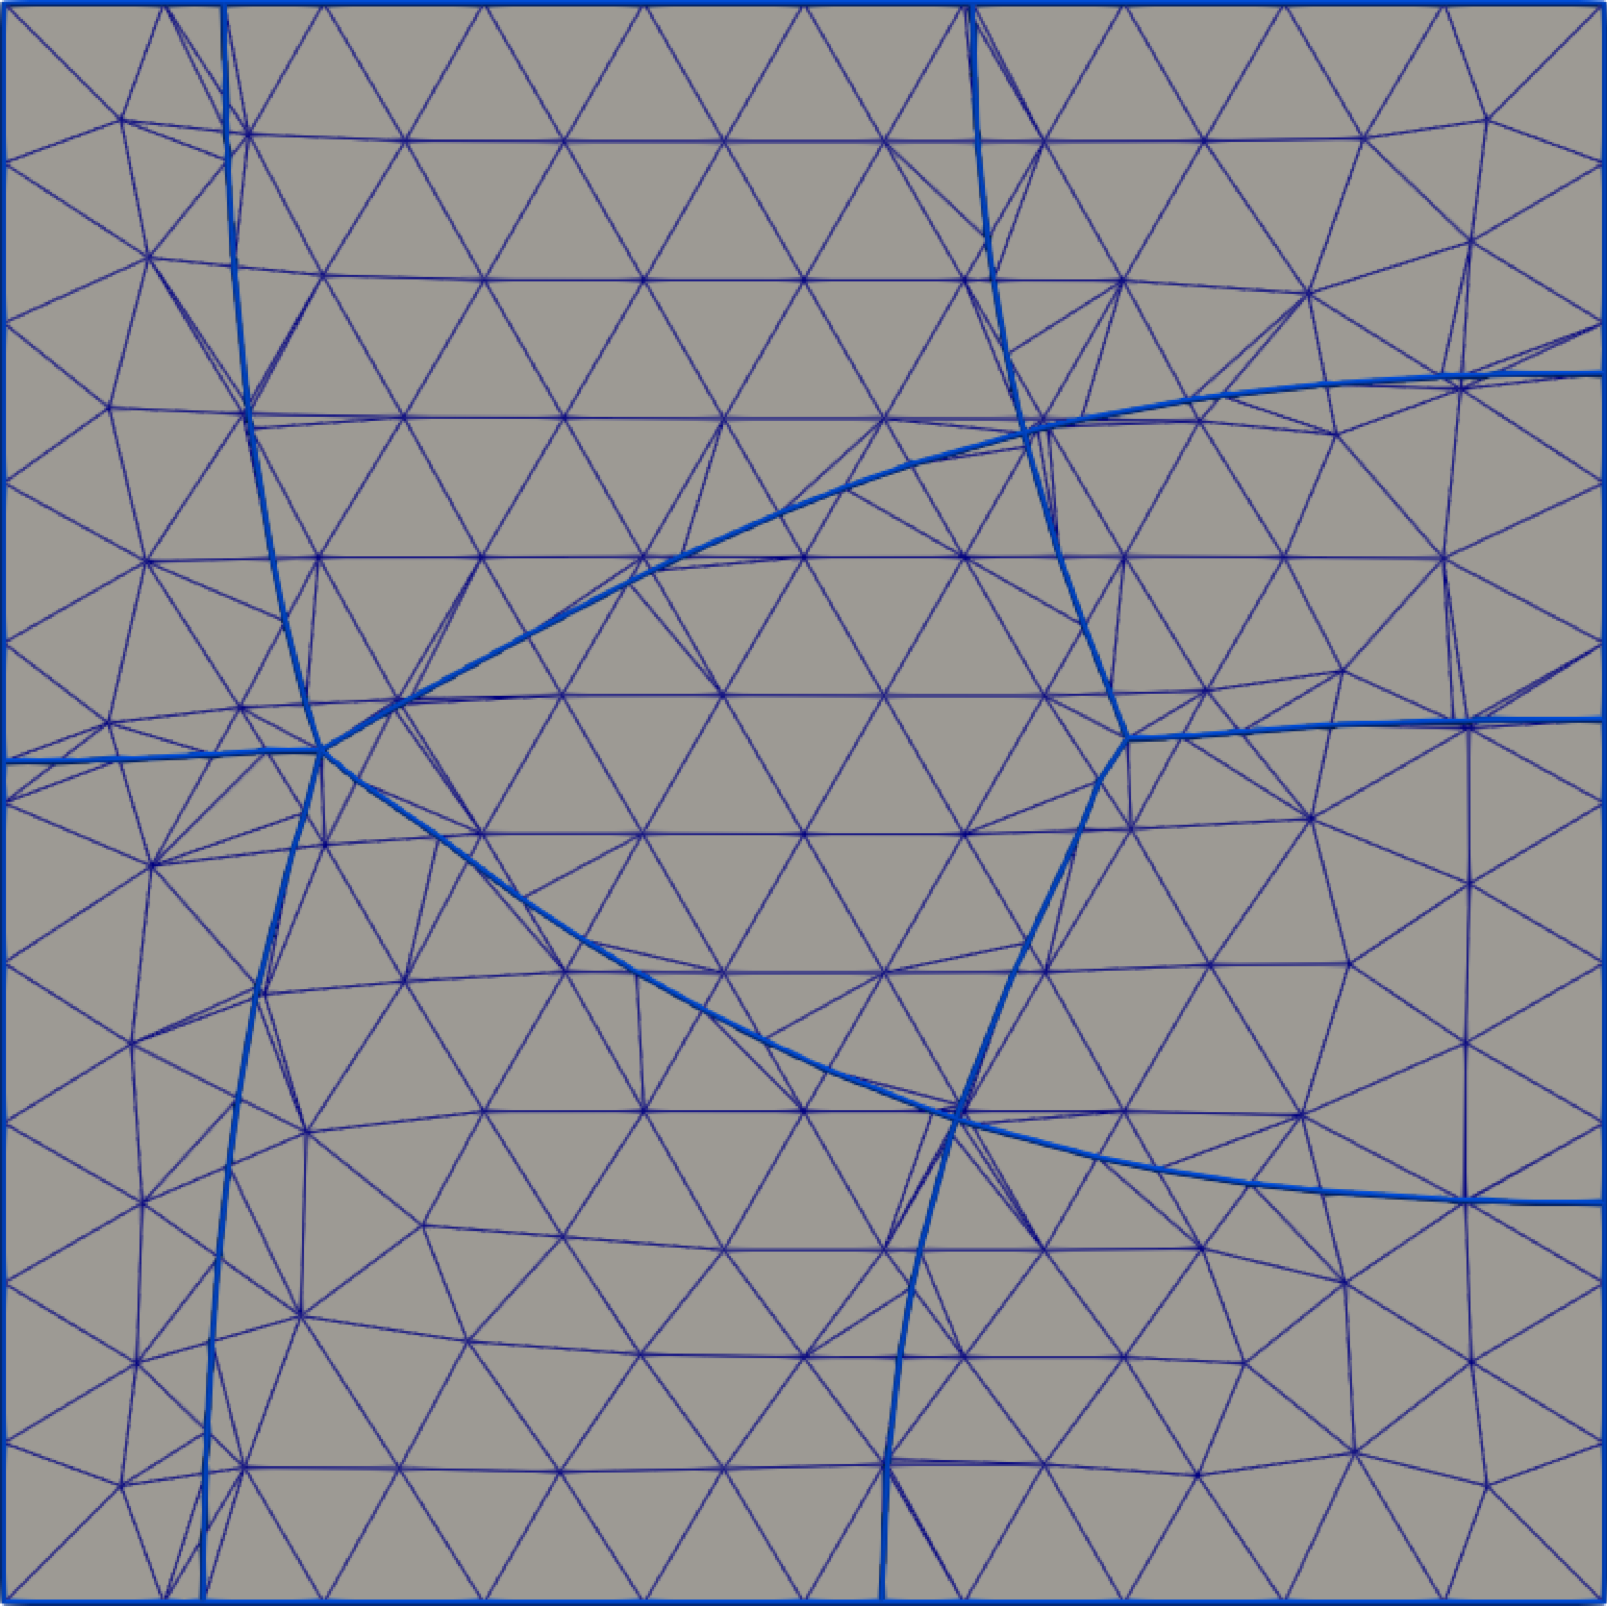
\includegraphics[width=\textwidth]{images/eclatement_2.pdf}
    %\caption{Insertion de $D$.}
    %\label{fig:quad_eclatement}
\end{subfigure}
\hfill
\begin{subfigure}{0.49\textwidth}
    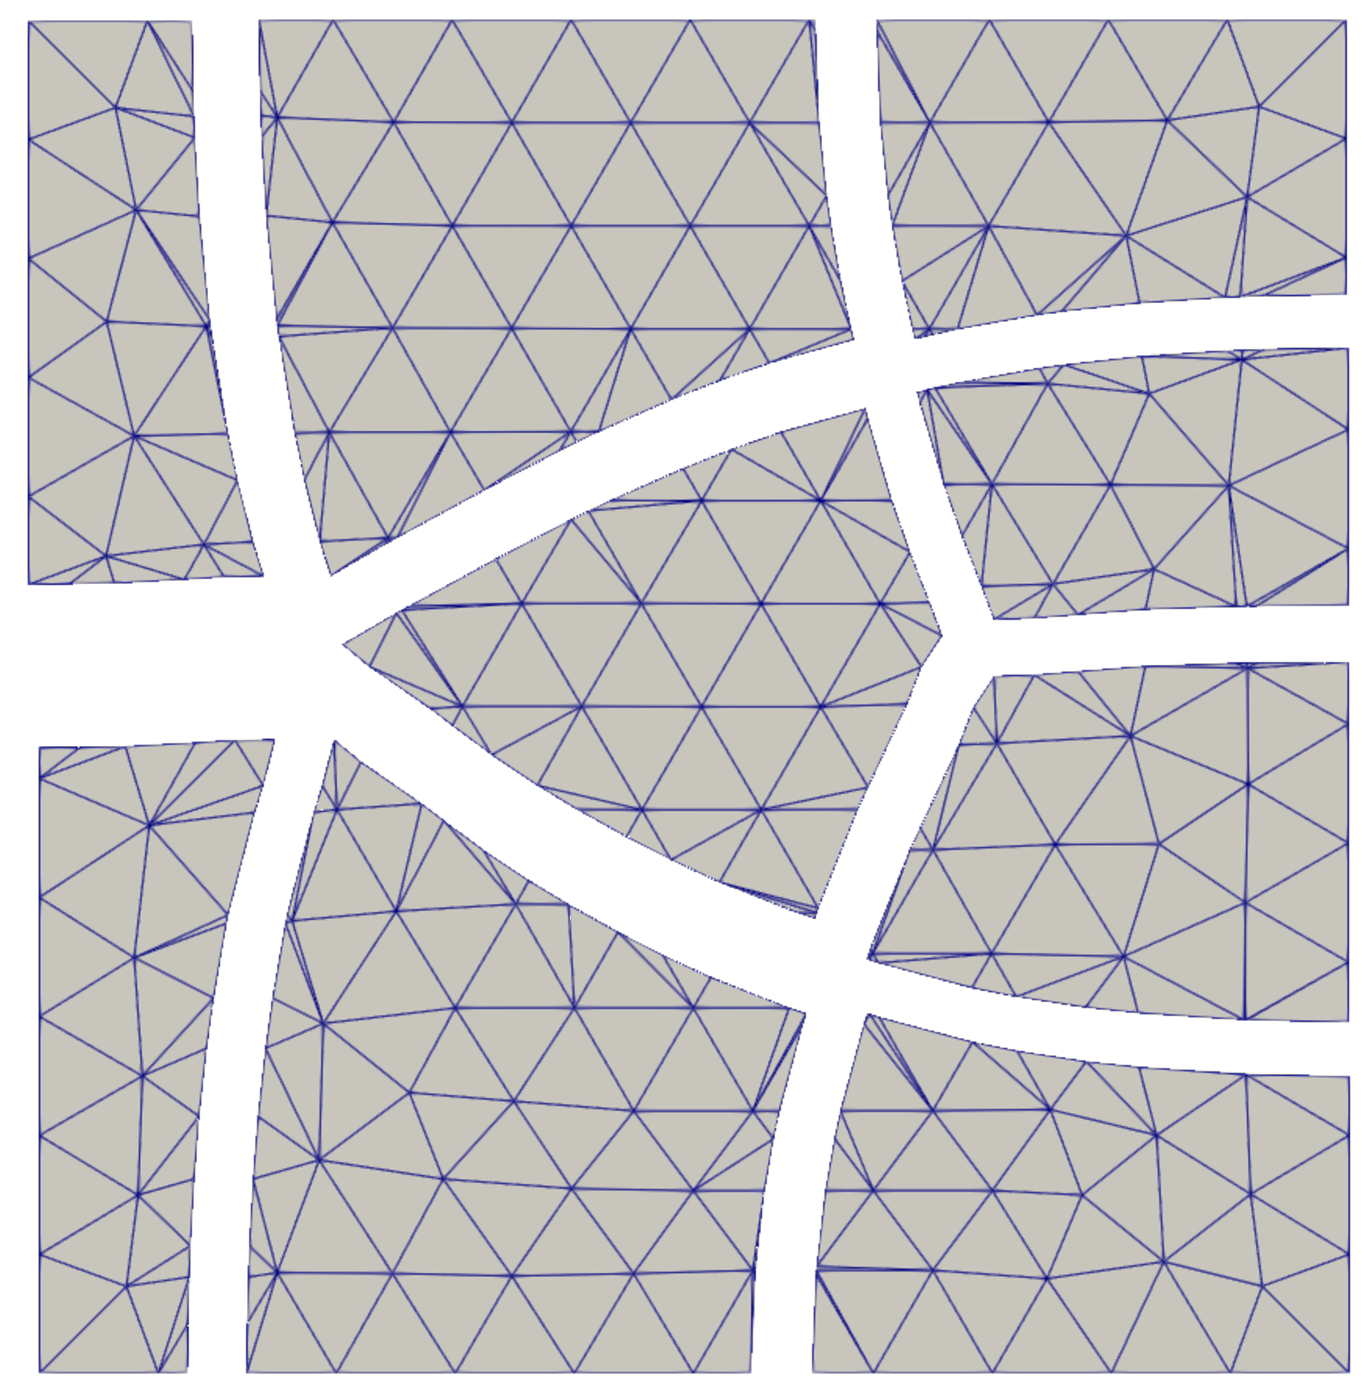
\includegraphics[width=\textwidth]{images/eclatement_3.pdf}
    %\caption{Insertion de $E$.}
    %\label{fig:quad_carre}
\end{subfigure}
\caption{Extraction des régions en tant que sous-maillages.}
\label{fig:eclatement}
\end{figure}


\section{Génération du maillage quadrilatéral}
\label{sec:gen_mesh_quad}

Nous nous tournons maintenant vers la génération du maillage quadrilatéral proprement dit. L'approche consiste à réaliser le maillage de manière indépendante pour chaque partition construite lors du processus de partitionnement du domaine (voir section \ref{sec:partitionnement_omega_h}). Nous désignerons par \emph{blocs} ces partitions dans la suite. Il est impératif que chaque bloc soit constitué de 4 côtés, c'est-à-dire que ses bords doivent avoir été formés par exactement 4 séparatrices. En l'absence de cette condition, comme illustré sur la figure \ref{fig:echec_partitionnement}, les approches utilisées ultérieurement pour générer le maillage ne fonctionneront pas correctement. Les conditions pour garantir que le partitionnement sera constitiué de blocs de quatres côtés sont abordés dans la section \ref{subsec:analyse_convergence}. Supposons que le partitionnement a bien généré des blocs de quatre côtés et définissons un pas de maille pour le maillage à générer. Pour chaque séparatrice nous déterminons le nombre de nœuds uniformément répartis sur celle-ci par rapport au pas de maille défini. Cependant, pour mailler un bloc, il est nécessaire de s'assurer que ses côtés opposés sont appariés deux à deux.

\begin{figure}[h!]
\centering
\begin{subfigure}{0.49\textwidth}
    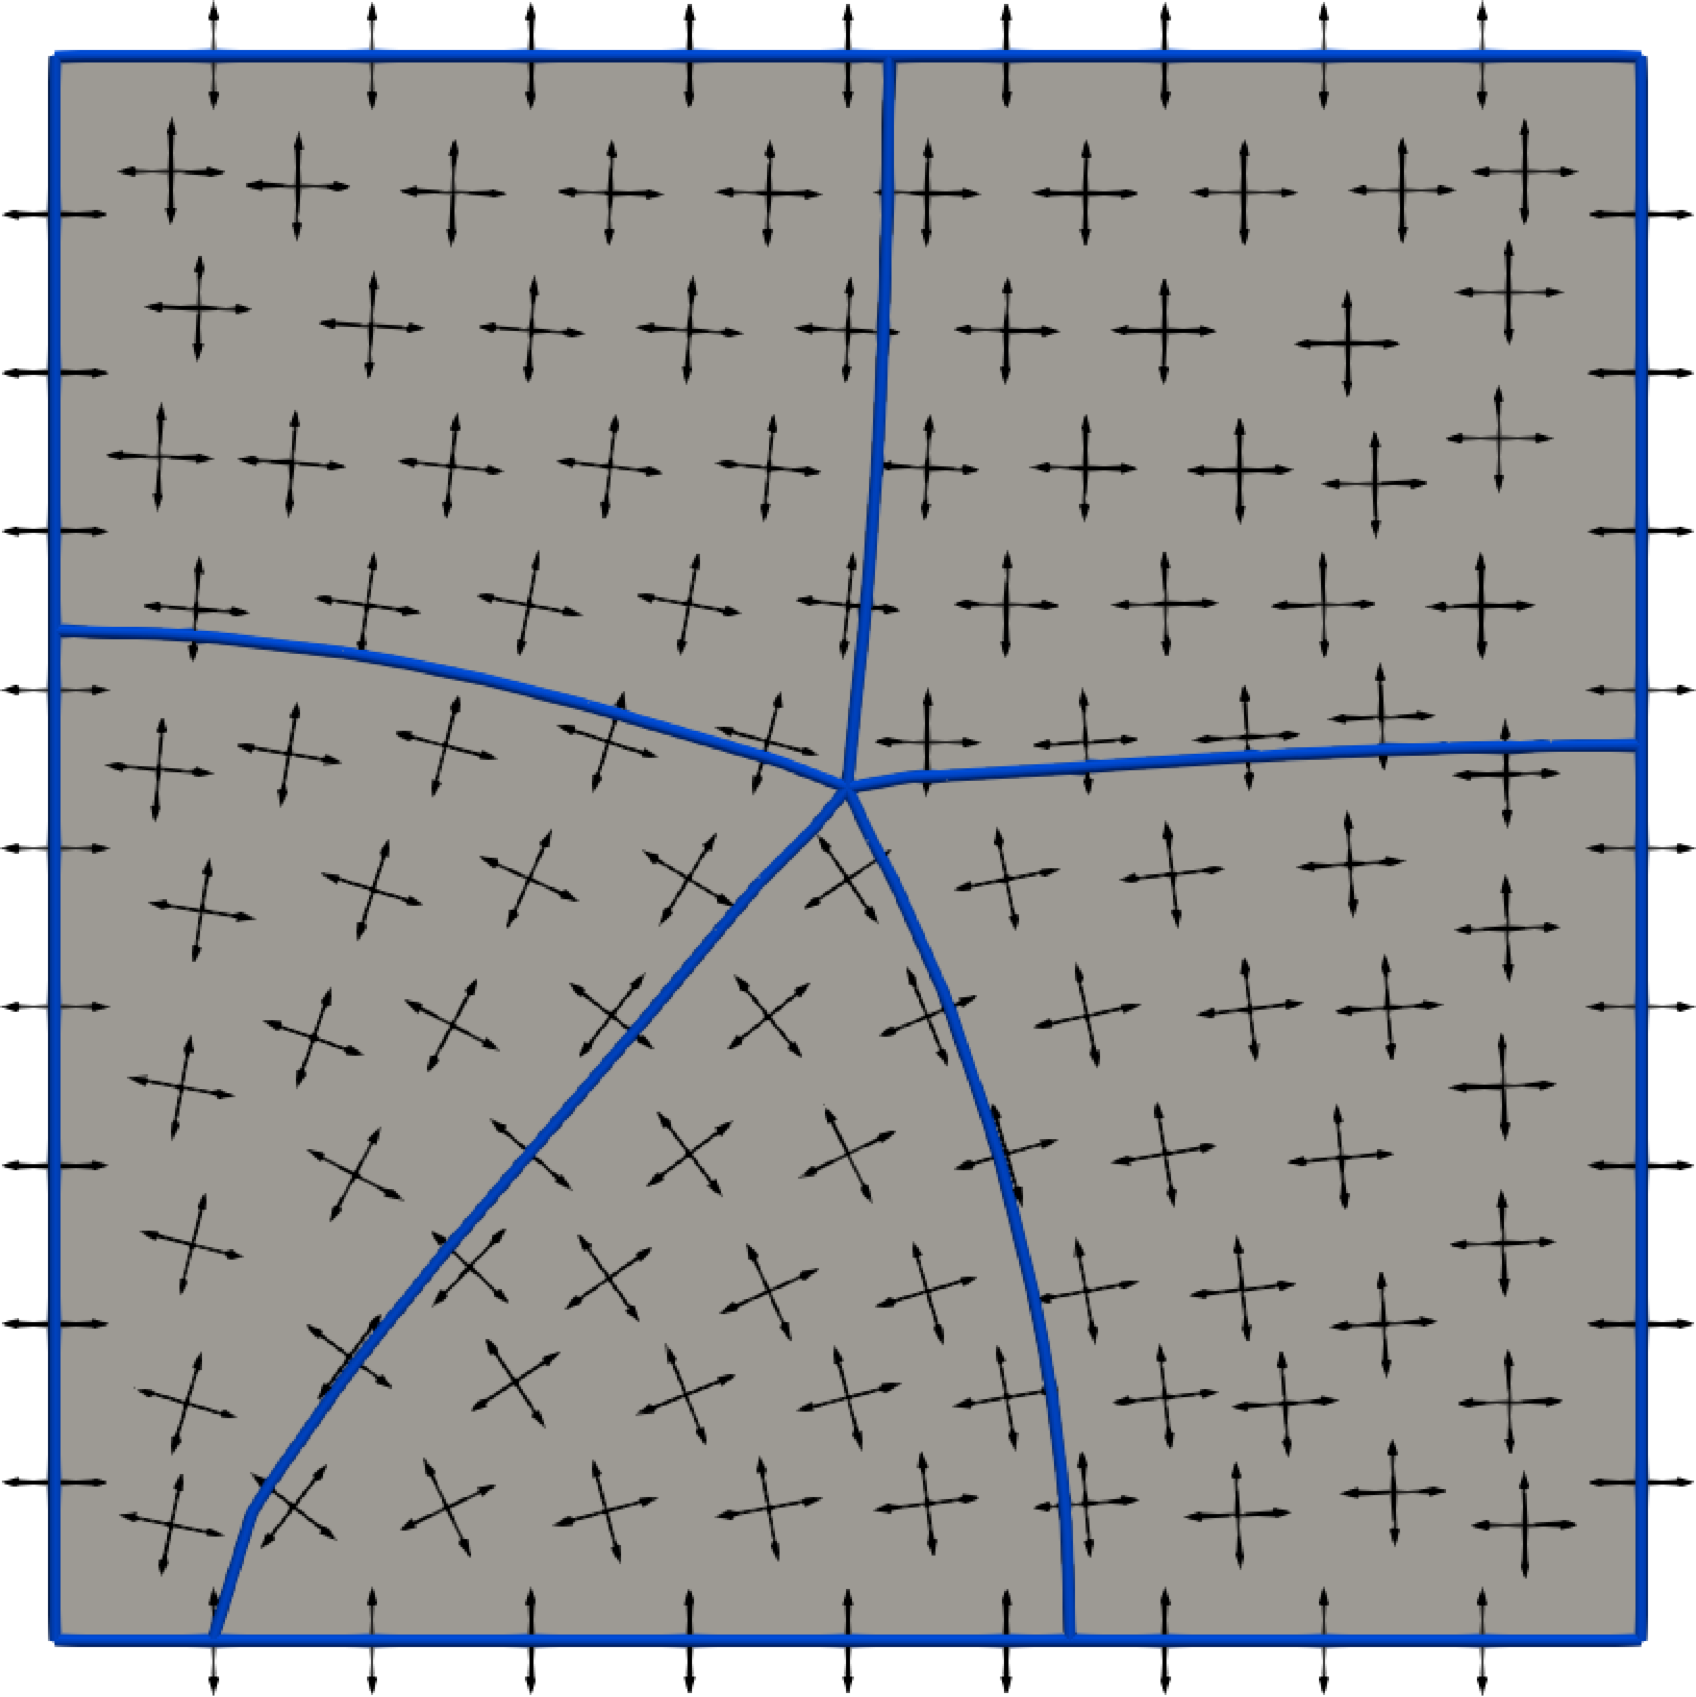
\includegraphics[width=\textwidth]{images/echec_partitionnement_1.pdf}
    %\caption{Insertion de $D$.}
    %\label{fig:quad_eclatement}
\end{subfigure}
\hfill
\begin{subfigure}{0.49\textwidth}
    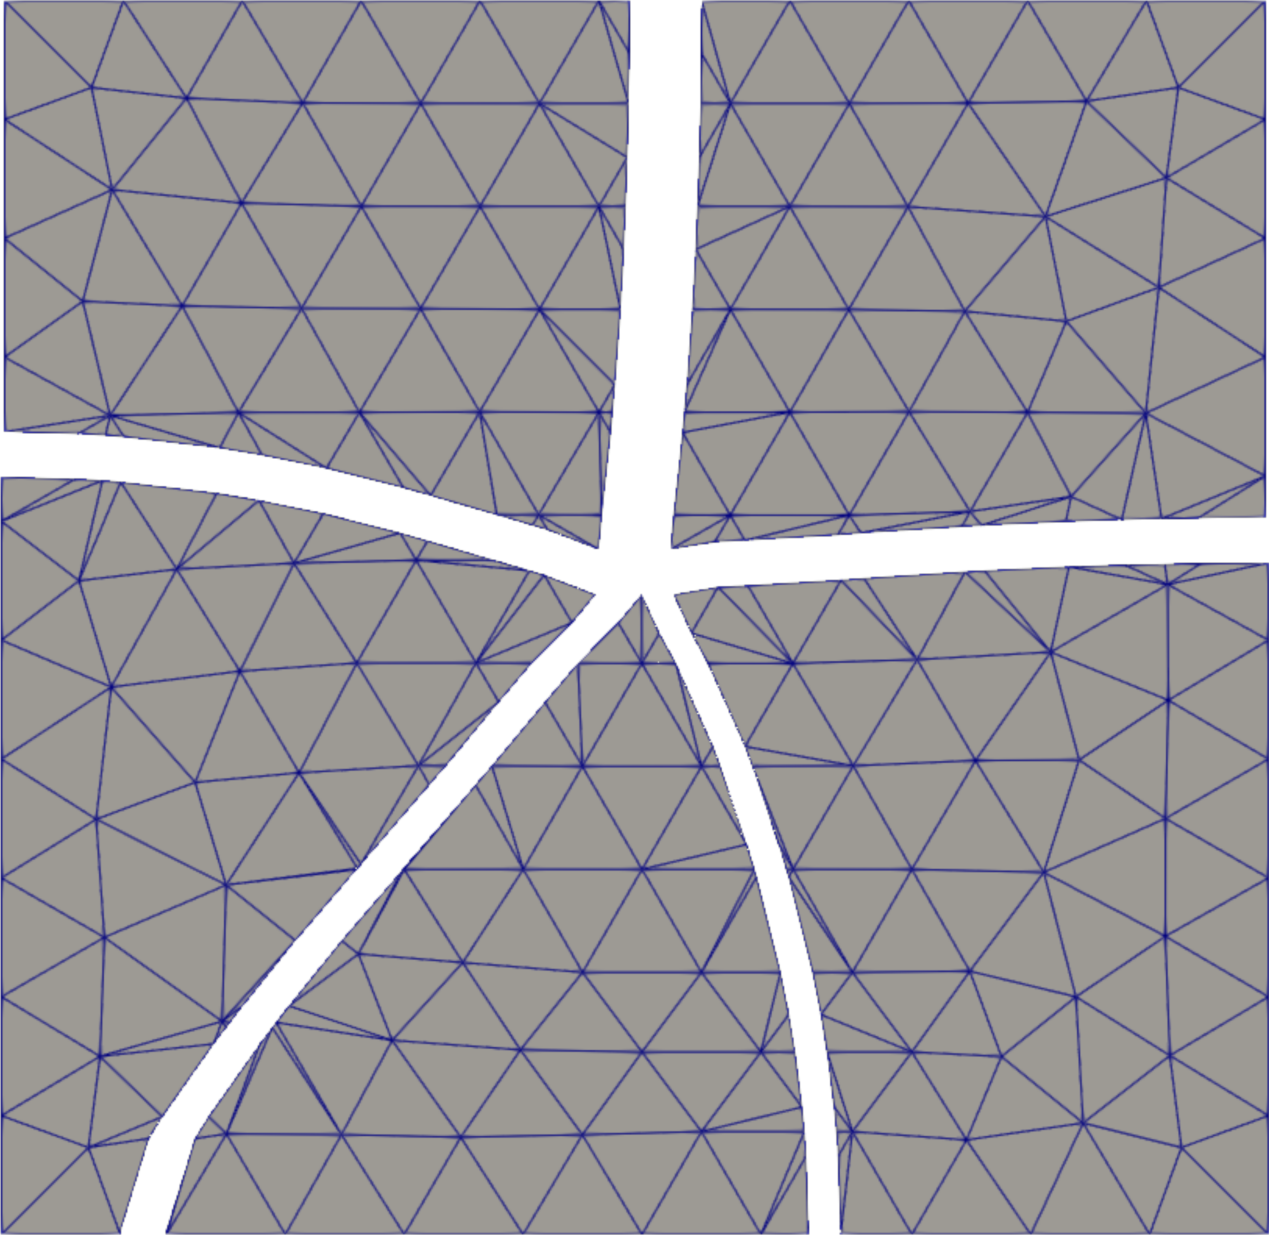
\includegraphics[width=\textwidth]{images/echec_partitionnement_2.pdf}
    %\caption{Insertion de $E$.}
    %\label{fig:quad_carre}
\end{subfigure}
\caption{Echec du Partitionnement. Toutes les partitions n'ont pas 4 côtés.}
\label{fig:echec_partitionnement}
\end{figure}

\subsection{Uniformisation}

Afin d'uniformiser la discrétisation, il est nécessaire de former des ensembles de séparatrices parallèles entre elles et de leur attribuer le même nombre de nœuds. Deux séparatrices opposées d'un même bloc seront dites \emph{parallèles}. Cette notion peut être étendue à l'ensemble du partitionnement par transitivité de la manière suivante : soient $SP_1$ et $SP_2$ deux séparatrices quelconques. On dira que $SP_1$ est parallèle à $SP_2$ s'il existe un bloc contenant $SP_1$, et que le côté opposé à $SP_1$ est parallèle à $SP_2$. L'algorithme ci-dessous permet de partitionner l'ensemble des séparatrices en sous-ensembles distincts de séparatrices parallèles.

\vspace{0.5cm}
\RestyleAlgo{ruled}
\begin{algorithm}[H]
\label{alg:separatrice_echantillonage}
\renewcommand{\algorithmcfname}{Algorithme}%
\SetAlgoLined
\Entree{Ensemble $SP$ des séparatrices}
\Sortie{Maillage local $T_{mesh}$ de $T$ contenant dans sa liste d'arêtes les segments des séparatrices inclus dans $T$}
\vspace{0.2cm}
\Repeter{$SP$ soit vide}
{
\vspace{0.2cm}
1.\quad Piocher un element de la liste\\[0.2cm]
2.\quad former l'ensemble des separatrices parallèle a cet element. Pour ce faire trouver les separatrices parallele à l'éléments puis recurcivement faire de même pour ce séparatrices jusqu'a ce qu'il n'y en ai plus\\[0.2cm]
3.\quad retirer ces elements de $SP$\\[0.2cm]
}
\vspace{0.2cm}
\caption{Assemblage de séparatrices parallèles.}
\end{algorithm}
\vspace{0.5cm}

Nous présentons sur la figure \ref{fig:separatrice_echantillonage} un exemple d'application de l'algorithme \ref{alg:separatrice_echantillonage}, où les séparatrices parallèles entre elles sont identifiées par la même couleur. Ensuite, il est possible d'assigner un nombre uniforme de nœuds à ces séparatrices en calculant la moyenne, le maximum ou le minimum du nombre de nœuds précédemment déterminé pour chaque séparatrice. Les côtés opposés de chaque bloc ont alors le même nombre de nœuds, et nous pouvons procéder à la génération du maillage pour chaque bloc. Nous présentons dans la suite plusieurs méthodes pour ce faire.

\begin{figure}[h!]
\centering
\begin{subfigure}{0.49\textwidth}
    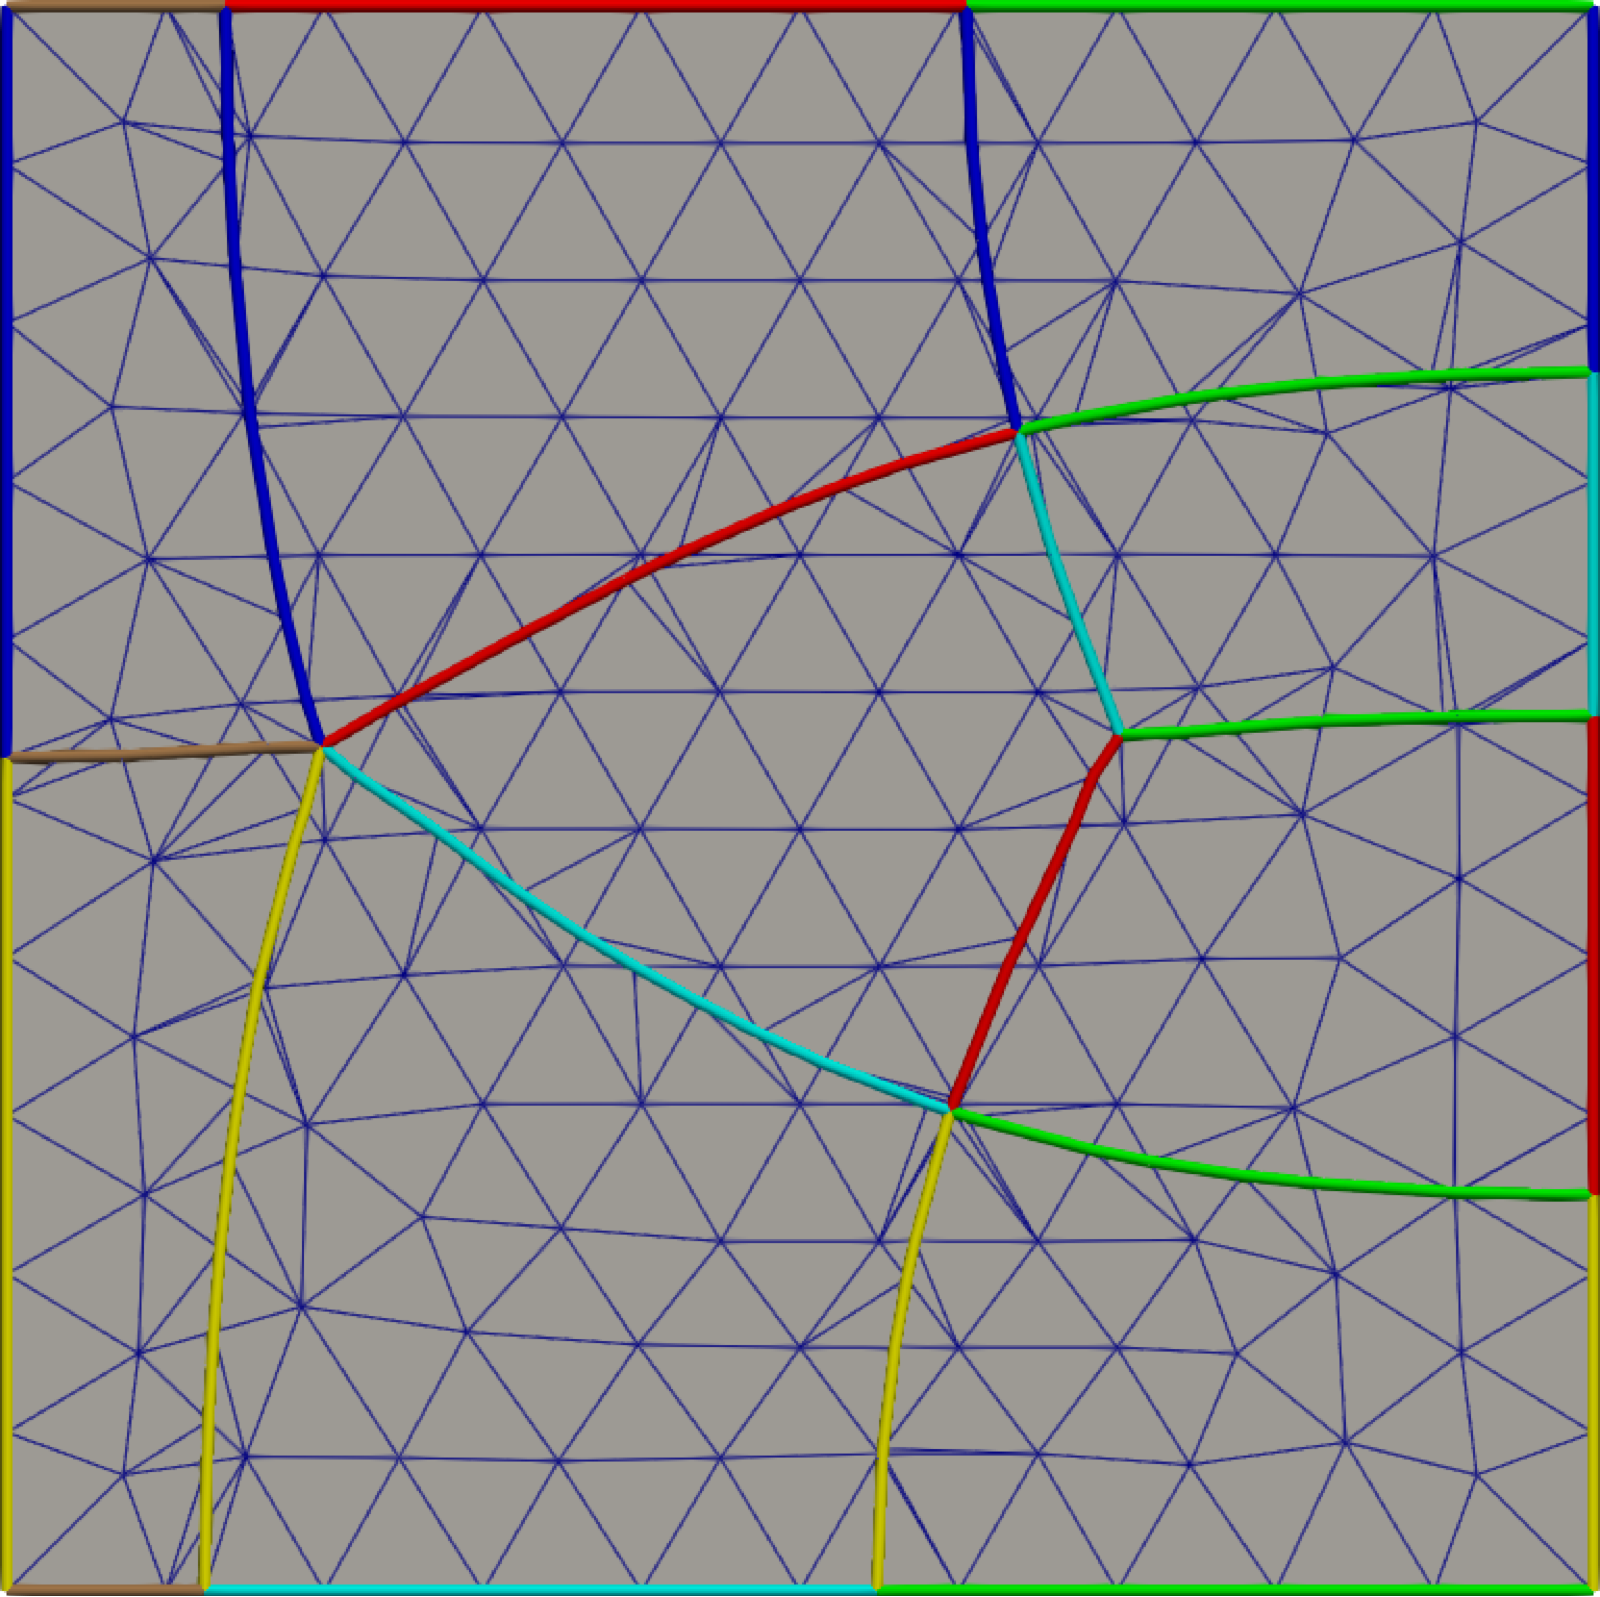
\includegraphics[width=\textwidth]{images/separatrice_echantillonage_1.pdf}
    %\caption{Insertion de $D$.}
    %\label{fig:quad_eclatement}
\end{subfigure}
\hfill
\begin{subfigure}{0.49\textwidth}
    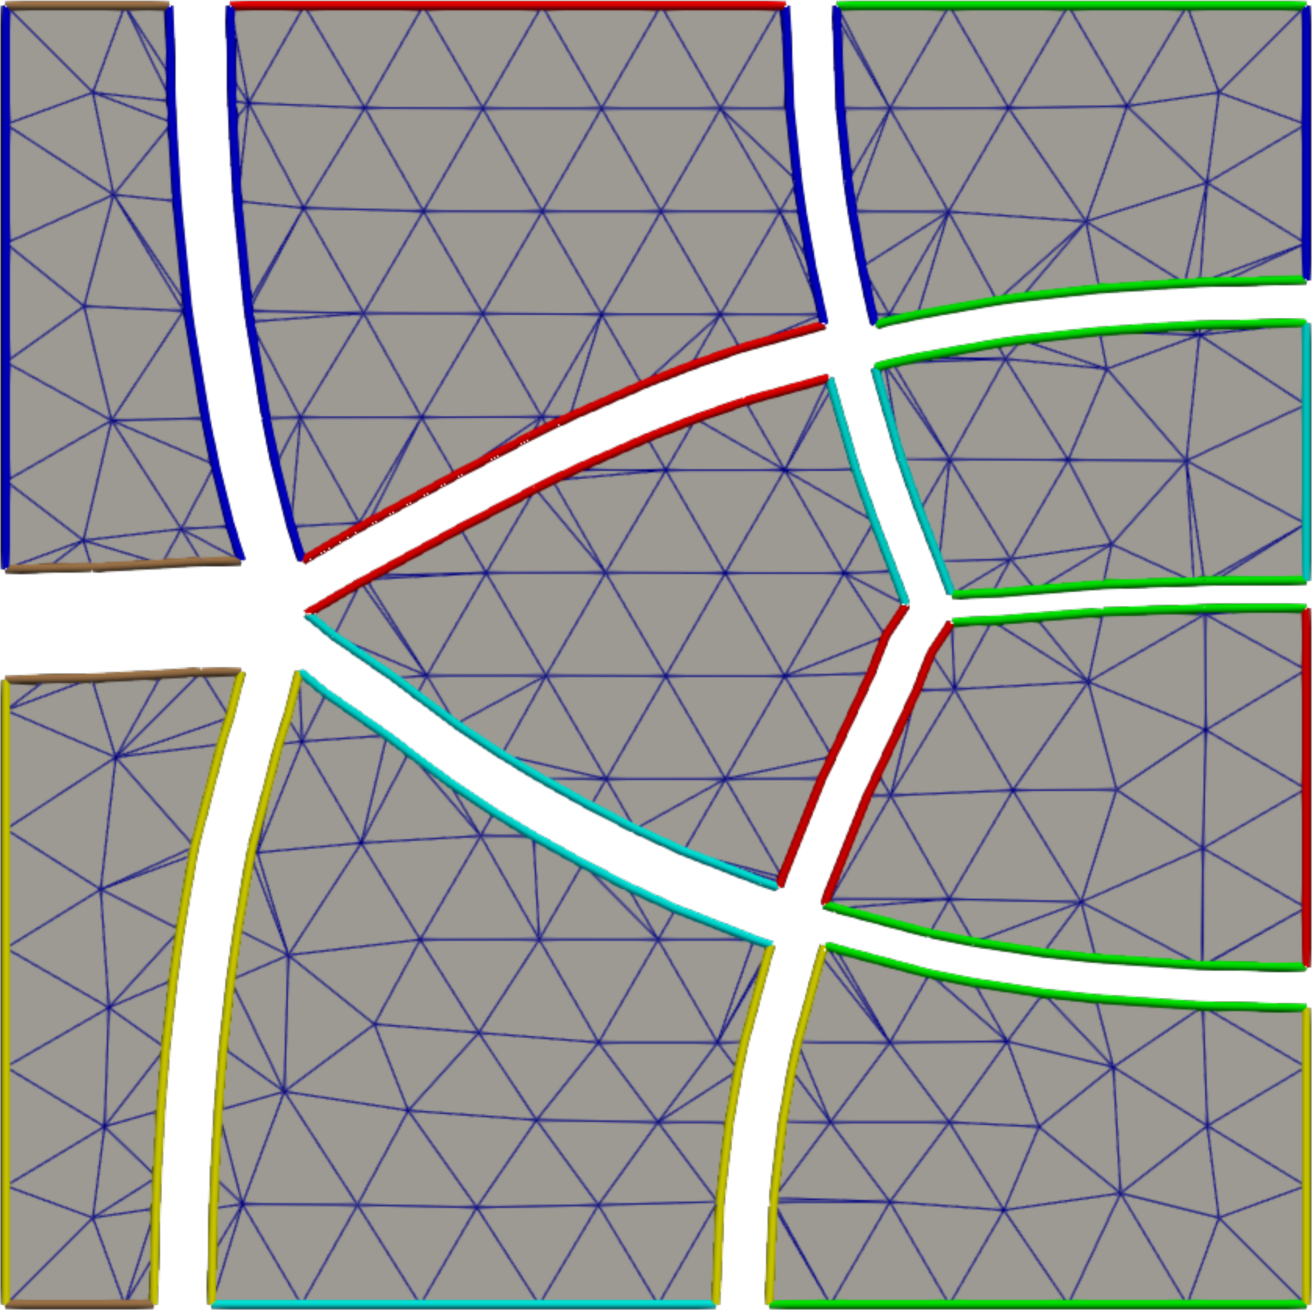
\includegraphics[width=\textwidth]{images/separatrice_echantillonage_2.pdf}
    %\caption{Insertion de $E$.}
    %\label{fig:quad_carre}
\end{subfigure}
\caption{Exemple d'identification de séparatrices parallèles : les séparatrices de même couleur sont parallèles.}
\label{fig:separatrice_echantillonage}
\end{figure}

\subsection{Interpolation transfinie}

De façon générale, il s'agit de construire une quadrangulation structurée $\mathcal{C}^0$-continue d'un quadrilatère dans $\mathbb{R}^d$ \cite{cook1974body} dont nous notons les noeuds $(P_{ij})_{i\in\llbracket 1, n\rrbracket, j\in\llbracket 1, m\rrbracket}$ avec $P_{ij}^x$ et $P_{ij}^y$ désignant les coordonnées de $P_{ij}$ pour tout $i\in\llbracket 1, n\rrbracket$ et $j\in\llbracket 1, m\rrbracket$. Soient $C_i,~i\in\llbracket 1, 4\rrbracket$ les séparatrices représentant les côtés d'un bloc donné, numéroté dans le sens positif, et posons:\\
\begin{itemize}
 \item[$\bullet$] $P_{1j}$, $j\in\llbracket 1, m\rrbracket$ les $m$ noeuds de la discrétisation de la séparatrice $C_1$,\\
 \item[$\bullet$] $P_{im}$, $i\in\llbracket 1, n\rrbracket$ les $n$ noeuds de la discrétisation de la séparatrice $C_2$,\\
 \item[$\bullet$] $P_{nj}$, $j\in\llbracket 1, m\rrbracket$ les $m$ noeuds de la discrétisation de la séparatrice $C_3$,\\
 \item[$\bullet$] $P_{i1}$, $i\in\llbracket 1, n\rrbracket$ les $n$ noeuds de la discrétisation de la séparatrice $C_4$.\\
\end{itemize}

 On se donne une quadrangulation uniforme du carré unité dont les nœuds sont notés $p_{ij}$ pour tout $i\in\llbracket 1, n\rrbracket$ et $j\in\llbracket 1, m\rrbracket$. Ces points sont ensuite reportés sur la partition via la transformation $T:p_{ij}\mapsto P_{ij}$ telle que :

$$
P_{ij}^x=(1-p_{ij}^x)P_{1j}^x+p_{ij}^xP_{mj}^x+(1-p_{ij}^y)P_{i0}^x+p_{ij}^y P_{in}^x-
\begin{bmatrix}
(1-p_{ij}^x), p_{ij}^x
\end{bmatrix}
\begin{bmatrix}
P_{00}^x&P_{mn}^x\\\\
P_{m0}^x&P_{0n}^x
\end{bmatrix}
\begin{bmatrix}
(1-p_{ij}^y)\\\\
p_{ij}^y
\end{bmatrix},
$$

$$
P_{ij}^y=(1-p_{ij}^x)P_{1j}^y+p_{ij}^xP_{mj}^y+(1-p_{ij}^y)P_{i0}^y+p_{ij}^y P_{in}^y-
\begin{bmatrix}
(1-p_{ij}^x), p_{ij}^x
\end{bmatrix}
\begin{bmatrix}
P_{00}^y&P_{mn}^y\\\\
P_{m0}^y&P_{0n}^y
\end{bmatrix}
\begin{bmatrix}
(1-p_{ij}^y)\\\\
p_{ij}^y
\end{bmatrix}.
$$

Cette opération réalise une transformation d'un maillage régulier dans l’espace paramétrique en un réseau de deux familles de lignes de maillage dans l’espace physique, avec les propriétés suivantes:\\
\begin{itemize}
 \item[$\bullet$]     La première et la dernière ligne de maillage de chaque famille épousent les frontières du domaine.\\
 \item[$\bullet$] Les lignes intermédiaires du maillage sont adaptées aux frontières et varient de manière monotone d’une frontière à l’autre.\\
 \item[$\bullet$] Le maillage n’est pas nécessairement orthogonal.\\
\end{itemize}
Nous illustrons le processus d'interpolation transfinie sur la figure \ref{fig:transfini}.

\begin{figure}[h!]
\centering
\begin{subfigure}{0.5\textwidth}
    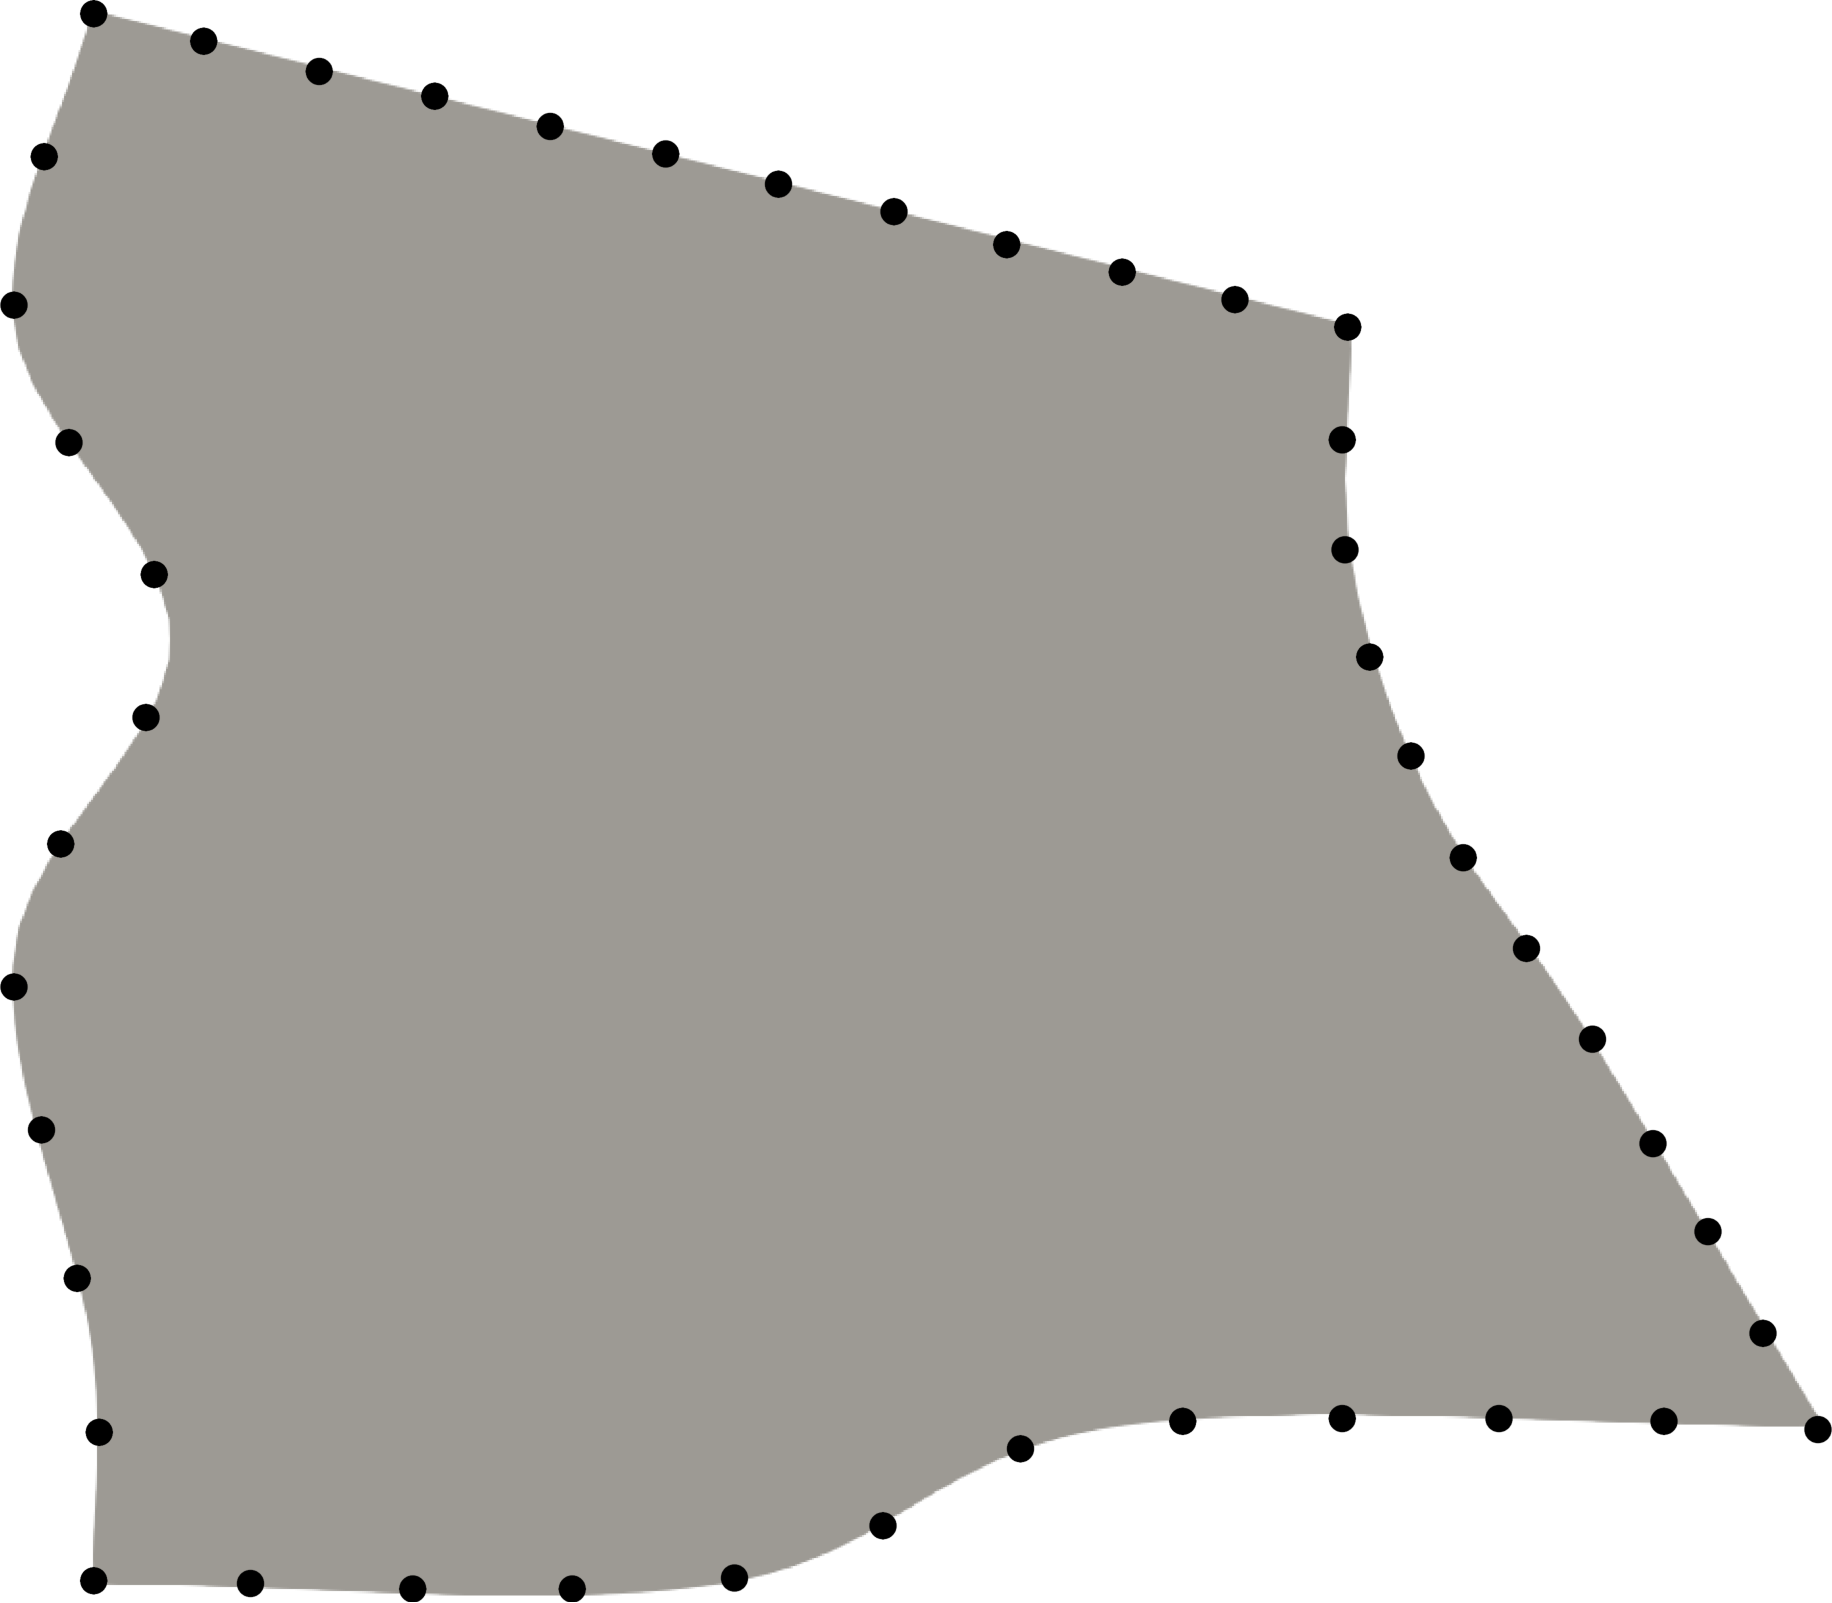
\includegraphics[width=\textwidth]{images/transfini_1.pdf}
    \caption{Discrétisation des séparatrices bordant le bloc.}
    \label{fig:transfini_1}
\end{subfigure}
\hfill
\begin{subfigure}{0.42\textwidth}
    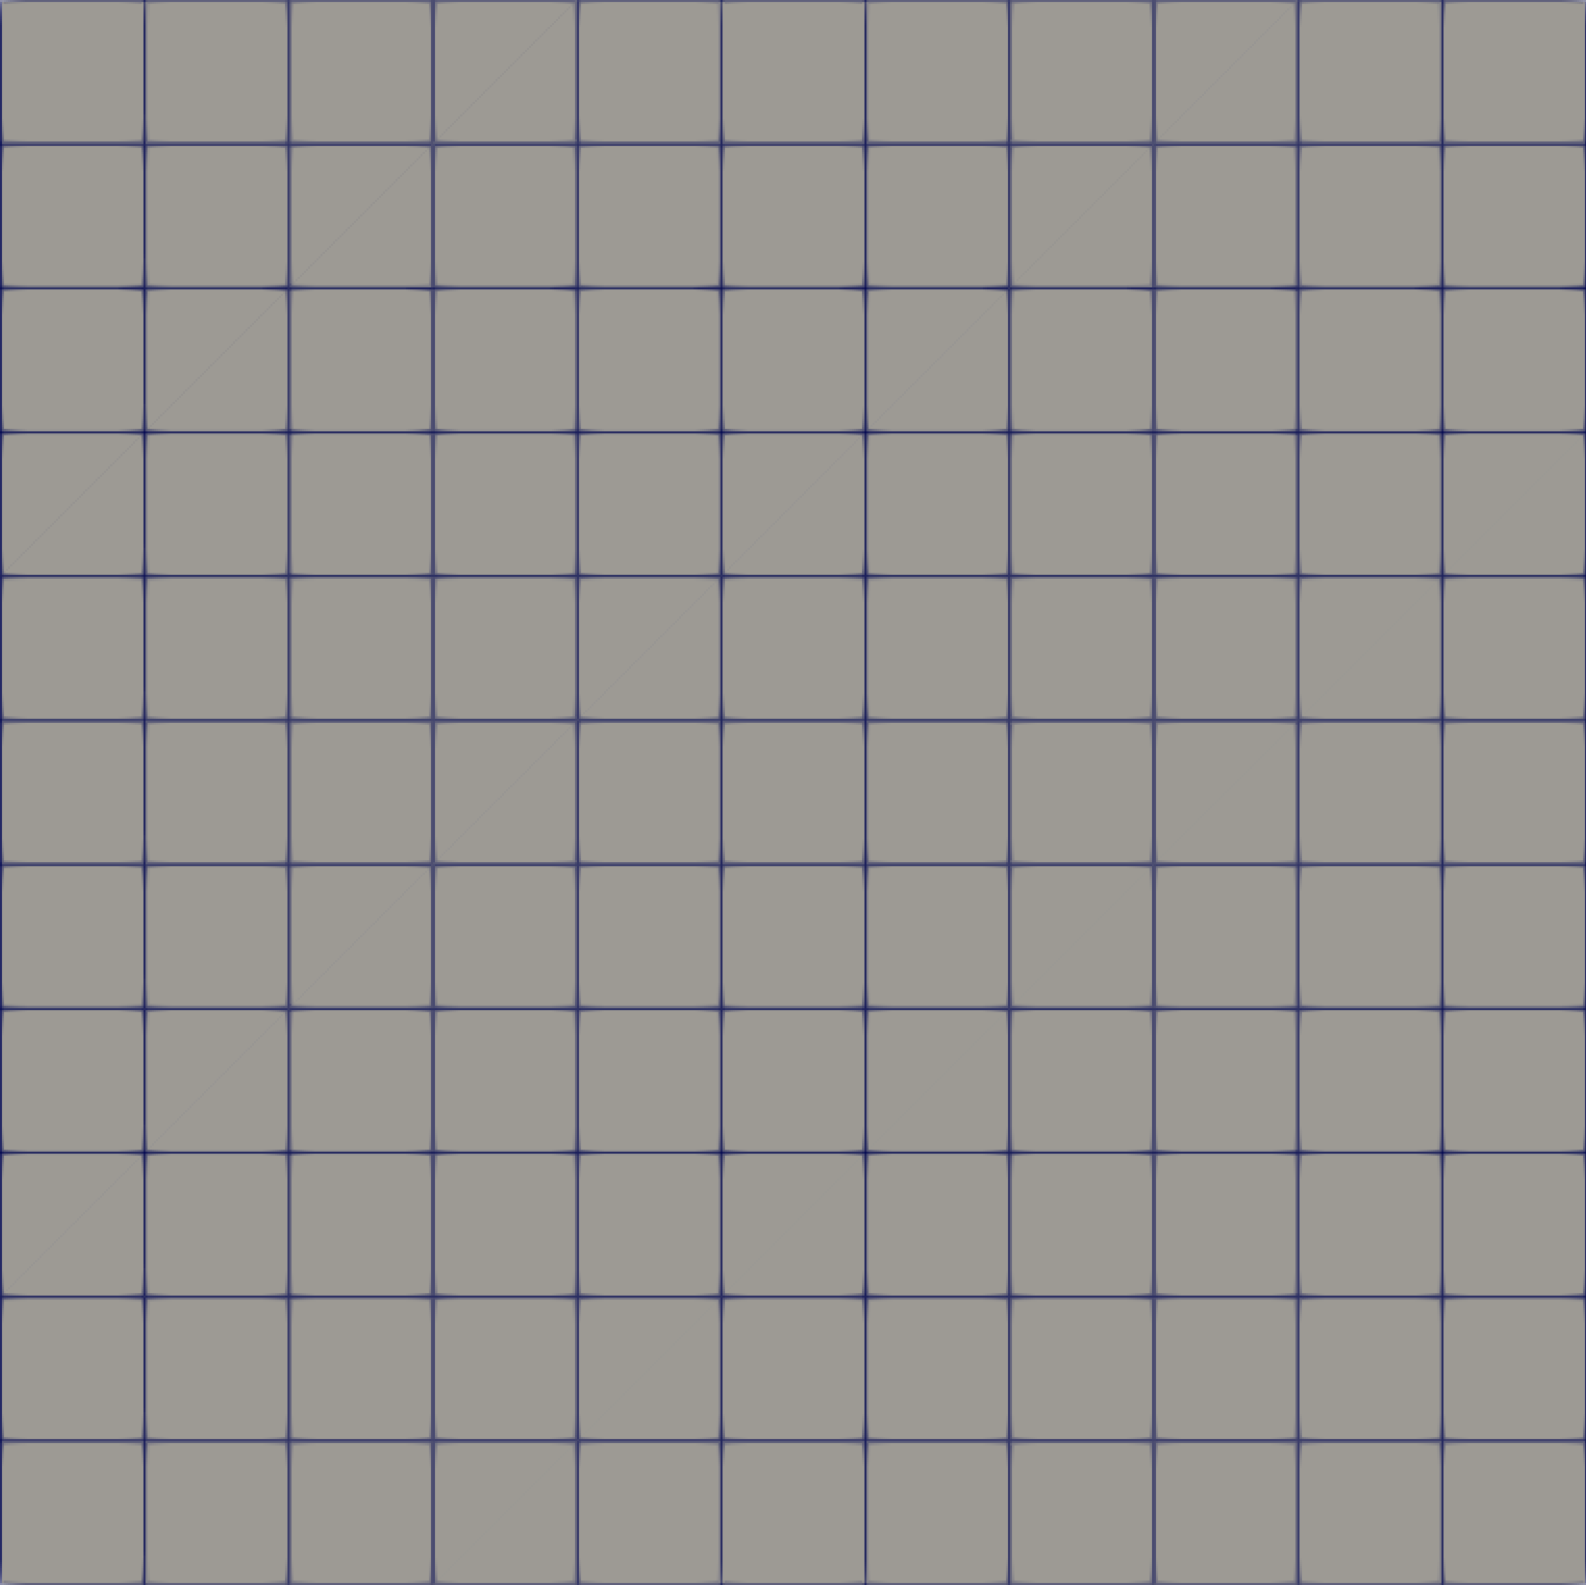
\includegraphics[width=\textwidth]{images/transfini_2.pdf}
    \caption{Maillage du carré unité.}
    \label{fig:transfini_2}
\end{subfigure}
\\[0.5cm]
\begin{subfigure}{0.5\textwidth}
    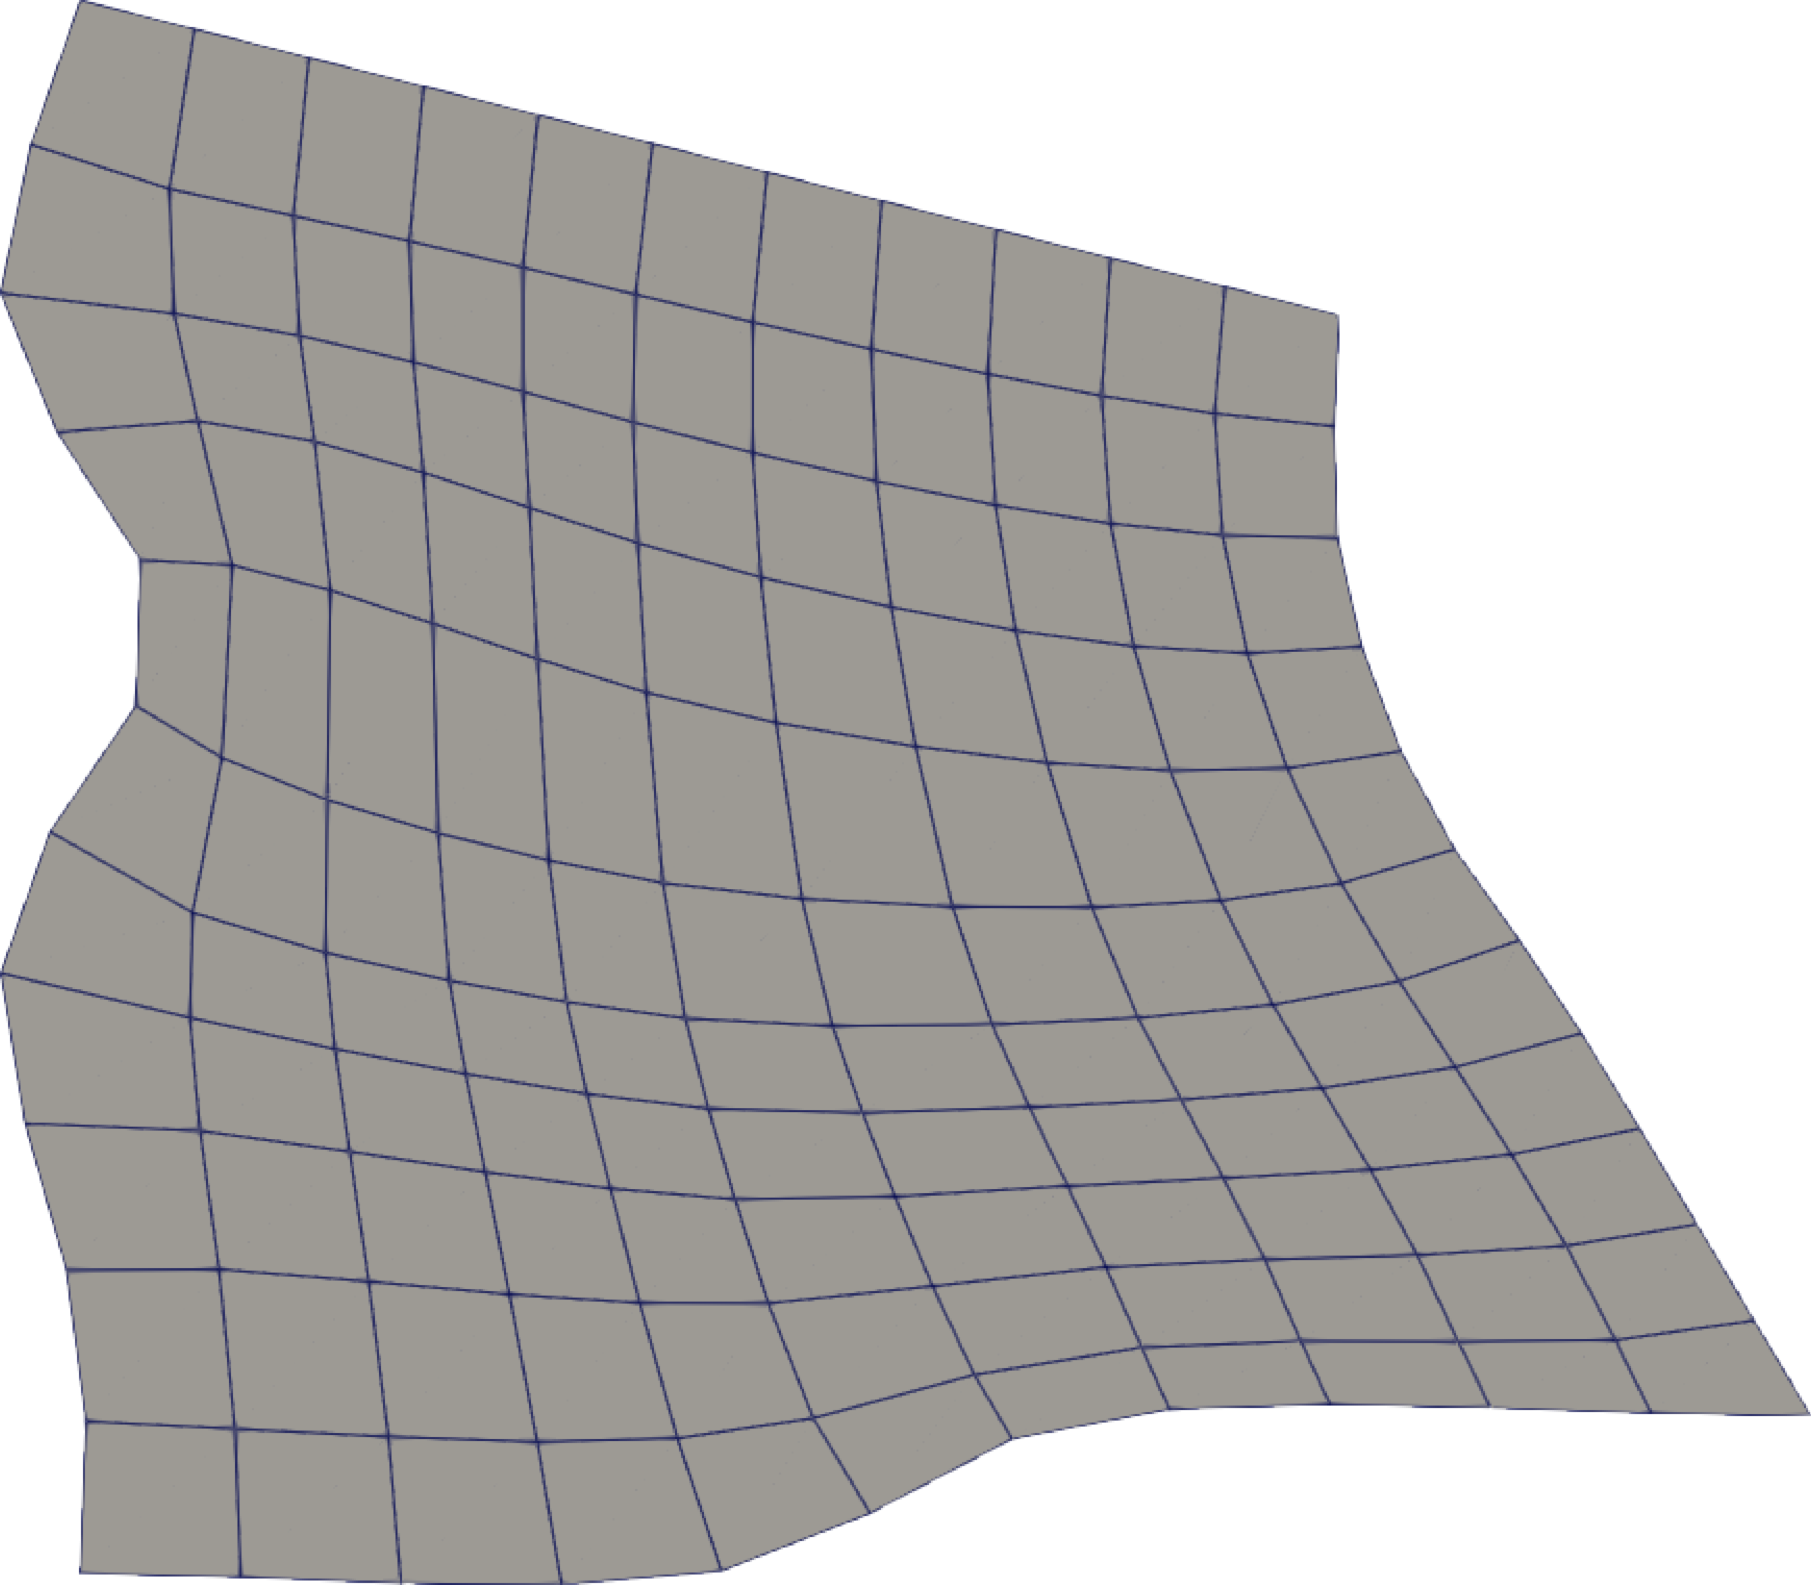
\includegraphics[width=\textwidth]{images/transfini_3.pdf}
    \caption{Maillage du bloc par transformation du maillage du carré unité (interpolation transfinie).}
    \label{fig:transfini_3}
\end{subfigure}
\caption{Illustration du processus d'interpolation transfinie.}
\label{fig:transfini}
\end{figure}



\subsection{Maillage par tracé direct de lignes de champ dans le champ de croix}
Dans ce cas, l'idée consiste à utiliser directement le champ de croix restreint $\bar{u}_h$ au bloc que l'on manipule pour construire le maillage du bloc. Il est important de noter que ce champ restreint est bien aligné avec les bords du bloc, étant donné que ces bords sont précisément les séparatrices construites précédemment en intégrant le champ de croix.

Le maillage proprement dit suit alors le même principe. On trace des lignes de champ en intégrant le champ de croix dans la région délimitée par le bloc, en utilisant comme point de départ les points de discrétisation des séparatrices de bord. Les lignes de champ servent de guides pour définir la disposition des points du maillage. Les intersections de ces lignes sont considérées comme des nœuds du maillage, et les éléments du maillage sont construits en reliant ces nœuds. Deux possibilités se présentent alors : soit initier les lignes de champ à partir d'un bord et les intégrer vers le bord opposé, soit initier les lignes de champ à partir de tous les bords du bloc, puis fusionner les lignes de champs provenant de points opposés grâce à la méthode de fusion de lignes de champ présentée plus haut. Dans le premier cas, la qualité du maillage sera fortement dépendante de la qualité des lignes de champ tracées. On observe que les erreurs d'intégration font dévier la ligne de champ, et on se retrouve bien souvent avec un maillage complètement déformé et inhomogène. La deuxième approche semble plus efficace. La dépendance à l'intégration est atténuée par la fusion des lignes de champ. Nous présentons une illustration de cette méthode sur la figure \ref{fig:mesh_by_streamline}.

\begin{figure}[h!]
\centering
\begin{subfigure}{0.49\textwidth}
    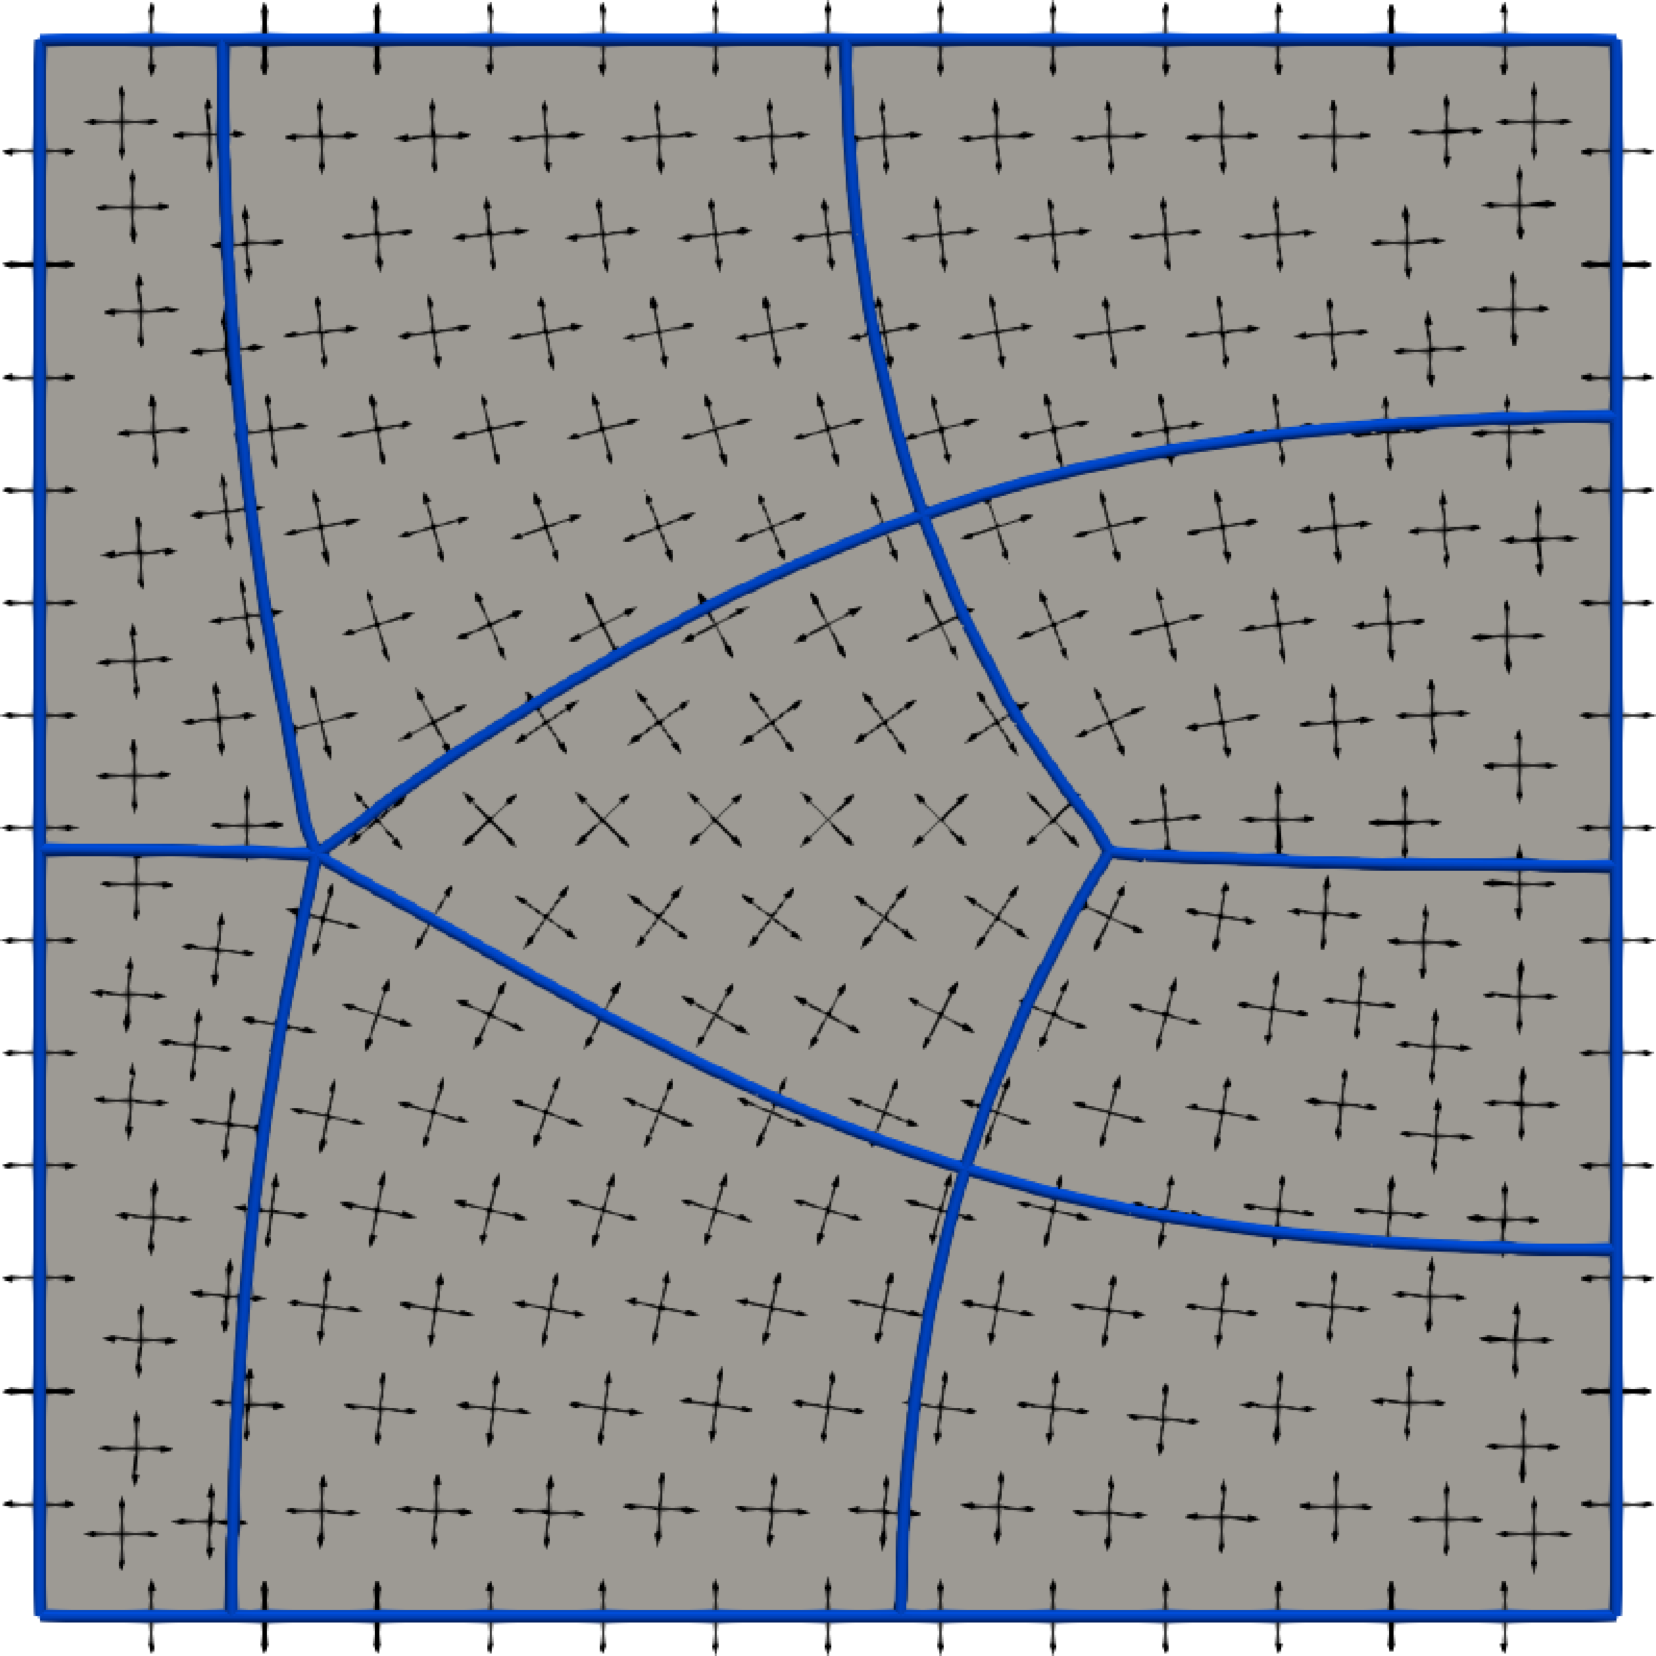
\includegraphics[width=\textwidth]{images/mesh_by_streamline_1.pdf}
    %\caption{Insertion de $D$.}
    \label{fig:mesh_by_streamline_1}
\end{subfigure}
\hfill
\begin{subfigure}{0.49\textwidth}
    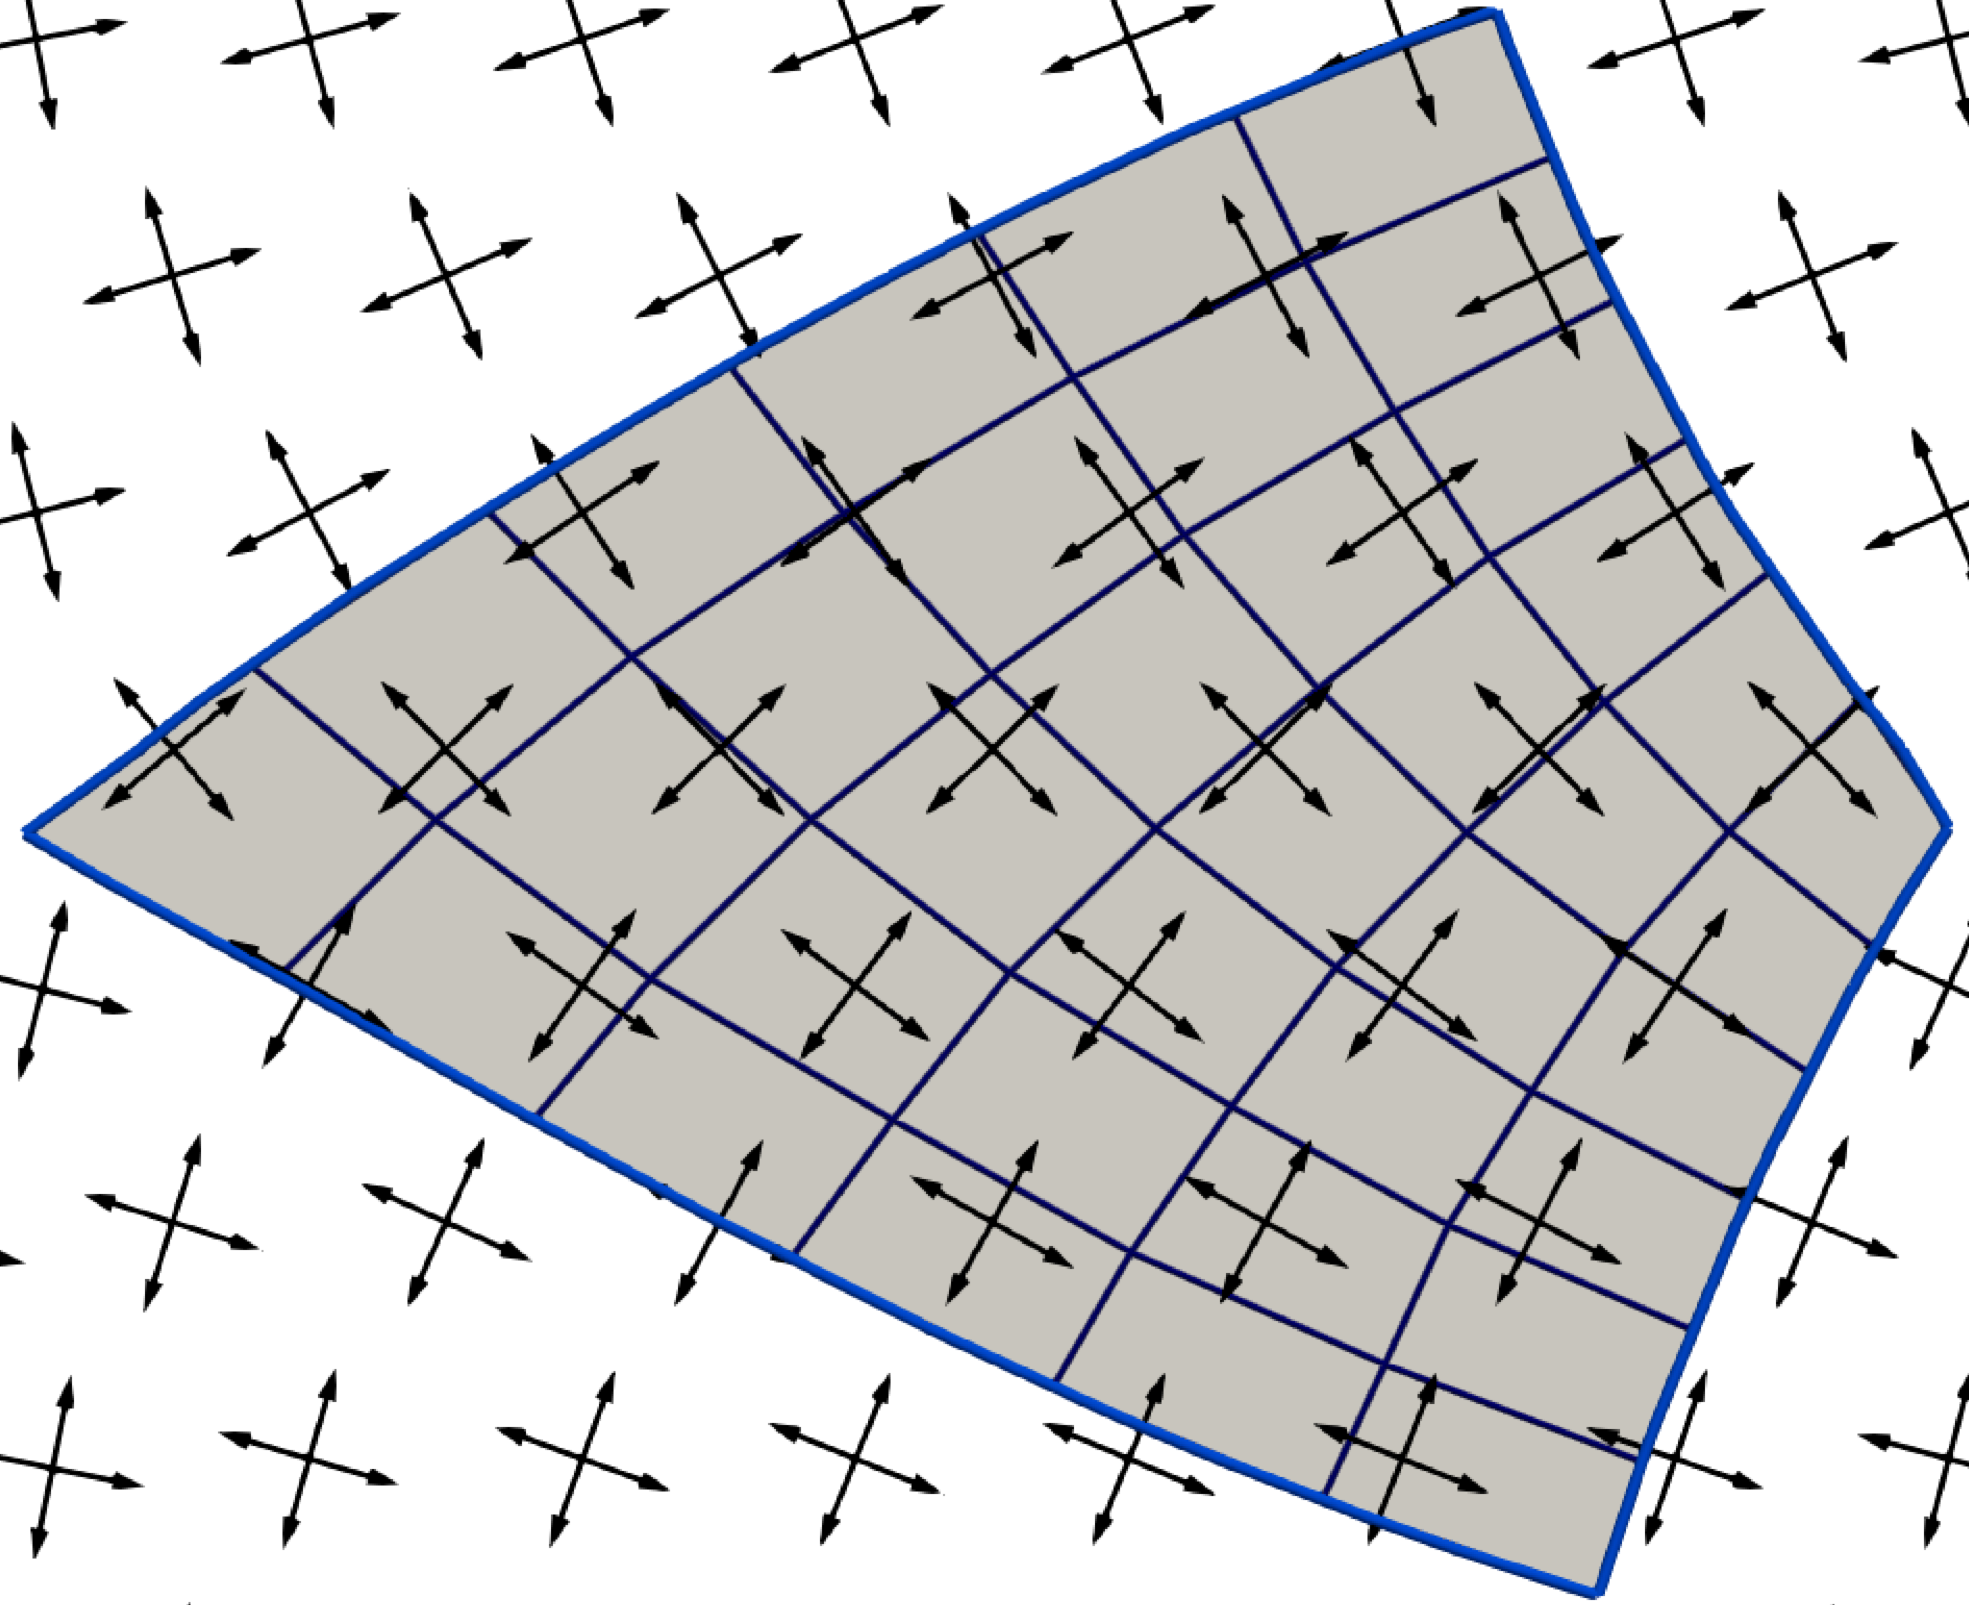
\includegraphics[width=\textwidth]{images/mesh_by_streamline_2.pdf}
    %\caption{Insertion de $E$.}
    \label{fig:mesh_by_streamline_2}
\end{subfigure}
\caption{Maillage par tracé direct de lignes de champ dans le champ de croix.}
\label{fig:mesh_by_streamline}
\end{figure}


\subsection{Méthode basée sur des EDP}
\label{method_based_edp}
Cette approche implique de générer le maillage pour un bloc spécifique en résolvant une Équation aux Dérivées Partielles (EDP), en utilisant la forme du contour du bloc comme condition aux bords. Considérons $C_i$, avec $i \in \llbracket 1, 4 \rrbracket$, comme les séparatrices (numérotées dans le sens positif) définissant les côtés d'un bloc particulier, noté $\Gamma$. Supposons que les côtés opposés $C_1$ et $C_3$ sont discrétisés en $m$ nœuds, tandis que les côtés opposés $C_2$ et $C_4$ sont discrétisés en $n$ nœuds. L'idée sous-jacente consiste à élaborer le maillage en construisant deux familles de lignes de niveau, l'une parallèle (au sens où elles ne s'intersectent pas) à $C_1$ et $C_3$, et l'autre orthogonale (au niveau des points d'intersection) à $C_2$ et $C_4$, et inversement pour l'autre famille de lignes de niveau. Soient $U$ et $V$ les solutions des équations suivantes :
$$
\left\{
\begin{array}{lcll}
\Delta U &=& 0 &\mbox{ dans }\Gamma,\\\\
U(p)&=& 0 & \mbox{ sur } C_1,\\\\
\displaystyle\frac{\partial U}{\partial n}(p)&=&0 & \mbox{ sur } C_2,\\\\
U(p)&=& n-1 & \mbox{ sur } C_3,\\\\
\displaystyle\frac{\partial U}{\partial n}(p)&=&0 & \mbox{ sur } C_4.
\end{array}
\right.
\quad\quad\quad\quad\quad\quad\quad\quad
\left\{
\begin{array}{lcll}
\Delta V &=& 0 &\mbox{ dans }\Gamma,\\\\
\displaystyle\frac{\partial V}{\partial n}(p)&=&0 & \mbox{ sur } C_1,\\\\
V(p)&=& m-1 & \mbox{ sur } C_2,\\\\
\displaystyle\frac{\partial V}{\partial n}(p)&=&0 & \mbox{ sur } C_3,\\\\
V(p)&=& 0 & \mbox{ sur } C_4.
\end{array}
\right.
$$
\[\]
Les lignes de niveau des champs scalaires $U$ et $V$ forment ainsi une grille régulière à partir de laquelle on peut déduire un maillage pour le bloc $\Gamma$. Pour ce faire, il suffit de considérer les lignes de niveau correspondant aux valeurs prises par les nœuds de discrétisation sur les bords de ces champs. Cela est illustré dans les figures \ref{fig:quad_equation_1}, \ref{fig:quad_equation_2} et \ref{fig:quad_equation_3}. Dans cet exemple, nous choisissons $m=n=12$. Les intersections des lignes de niveaux sont alors considérées comme des nœuds du maillage, et les éléments du maillage sont construits en reliant ces nœuds. Cependant, un tel maillage peut être insatisfaisant car on observe que les cellules ne sont pas homogènes. De plus, les noeuds du bords ne correspondent pas forcément au discrétrisation des séparatrices ce qui entraîne un déphase des noeuds entre deux blocs voisins et donc une non-conformité du maillage. Pour remédier à cela, nous introduisons une grille régulière notée $(w_{ij})_{\substack{i\in\llbracket 1, n\rrbracket\\j\in\llbracket 1, m\rrbracket}}$  de taille $n\times m$ à partir duquel nous construisons le maillage sur le bloc. Pour ce faire:\\\\
Soit $C_1^k$, $k\in\llbracket 1, n\rrbracket$, les $n$ noeuds du côté $C_1$.\\\\
Soit $C_2^k$, $k\in\llbracket 1, m\rrbracket$, les $m$ noeuds du côté $C_2$.\\\\
Soit $C_3^k$, $k\in\llbracket 1, n\rrbracket$, les $n$ noeuds du côté $C_3$.\\\\
Soit $C_4^k$, $k\in\llbracket 1, m\rrbracket$, les $m$ noeuds du côté $C_4$.\\\\
Les nœuds $w_{ij}=(w_{ij}^x, w_{ij}^y)$ de la grille $(w_{ij})_{\substack{i\in\llbracket 1, n\rrbracket\\j\in\llbracket 1, m\rrbracket}}$ sont alors  donnés par:
\begin{equation}
w_{ij}=
\left\{
\begin{array}{ll}
(U(C_1^j), V(C_1^j)),&\mbox{ pour } j=1 \mbox{ et } i\in\llbracket 1, m\rrbracket\\\\
(U(C_2^i), V(C_2^i)),&\mbox{ pour } i=1 \mbox{ et } j\in\llbracket 1, n\rrbracket\\\\
(U(C_3^j), V(C_3^j)),&\mbox{ pour } j=1 \mbox{ et } i\in\llbracket 1, m\rrbracket\\\\
(U(C_4^i), V(C_4^i)),&\mbox{ pour } i=1 \mbox{ et } j\in\llbracket 1, n\rrbracket
\end{array}
\right.
\end{equation}
et pour tout $i\in\llbracket 2, n-1\rrbracket$ et $j\in\llbracket 2, m-1\rrbracket$, on a:
\begin{equation}
\left\{
\begin{array}{ll}
w_{ij}^x=w_{1j}^x+\displaystyle\frac{j-1}{m-1}\left(w_{nj}^x-w_{1j}^x\right),\\\\
w_{ij}^y=w_{i1}^y+\displaystyle\frac{i-1}{n-1}\left(w_{im}^x-w_{i1}^y\right).
\end{array}
\right.
\end{equation}
Le maillage (voir \ref{fig:quad_equation_4}) est alors obtenu en cherchant dans $\Gamma$ et en reliant les points $P_{ij}=(P_{ij}^x, P_{ij}^y)$, $i\in\llbracket 2, n-1\rrbracket$, $j\in\llbracket 2, m-1\rrbracket$ vérifiant:
\begin{equation}
\left\{
\begin{array}{lcl}
U(P_{ij})&=&w_{ij}^x,\\\\
V(P_{ij})&=&w_{ij}^y.
\end{array}
\right.
\end{equation}
Avec une discrétisation linéaire par morceaux des champs scalaires $U$ et $V$ sur un maillage triangulaire du bloc, les points $P_{ij}$, pour $i \in \llbracket 2, n-1 \rrbracket$ et $j \in \llbracket 2, m-1 \rrbracket$, peuvent être recherchés simultanément à l'intérieur de chaque triangle. Ainsi, $P_{ij}$, pour $i \in \llbracket 2, n-1 \rrbracket$ et $j \in \llbracket 2, m-1 \rrbracket$, appartient à un triangle $T$ ayant pour sommets $A_1$, $A_2$ et $A_3$ s'il existe $(\lambda_k)_{k \in \llbracket 1, 3 \rrbracket} \subset [0, 1]$ vérifiant le système suivant :
\begin{equation}
\left\{
\begin{array}{lcl}
\displaystyle\sum_{k=1}^3\lambda_k U_h(A_k) & = & w_{ij}^x,\\
\displaystyle\sum_{k=1}^3\lambda_k V_h(A_k) & = & w_{ij}^y,\\
\displaystyle\sum_{k=1}^3\lambda_k & = & 1,
\end{array}
\right.
\end{equation}
où $U_h$ et $V_h$ représentent les discrétisations de $U$ et $V$. Le point $P_{ij}$ est alors déterminé par $P_{ij}=\sum_{k=1}^3\lambda_kA_k$. Les points $P_{1j}$, $P_{i1}$, $P_{nj}$, $P_{im}$, avec $i \in \llbracket 1, n \rrbracket$ et $j \in \llbracket 1, m \rrbracket$, sont définis par les nœuds de discrétisation des points de bord.
\begin{figure}[h!]
\centering
\begin{subfigure}{0.455\textwidth}
    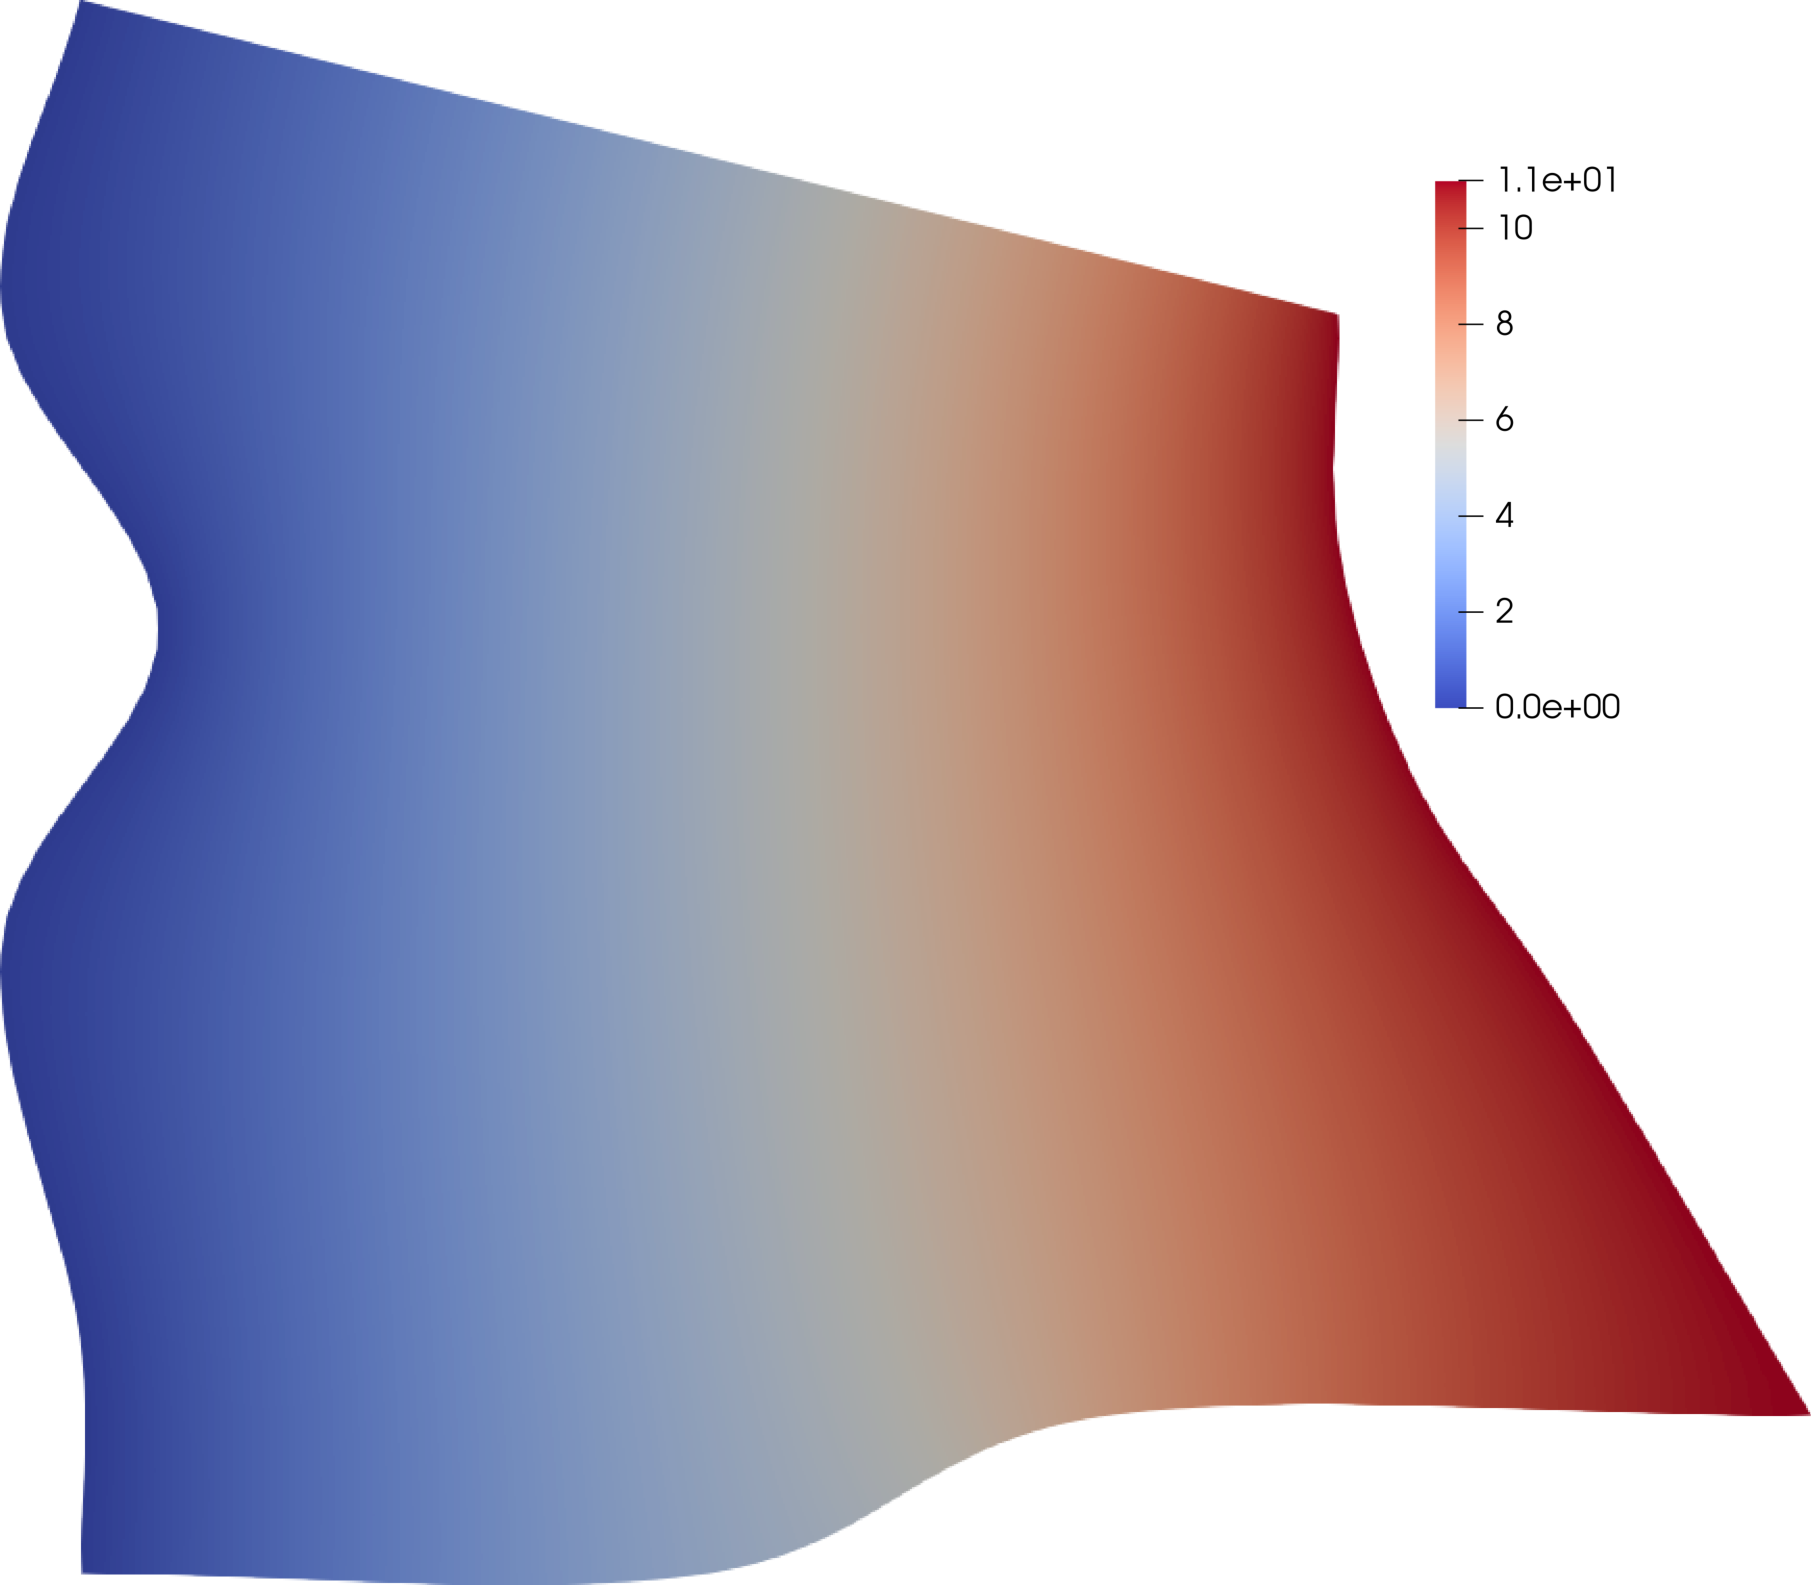
\includegraphics[width=\textwidth]{images/quad_equation_1.pdf}
    \caption{Champ scalaire $V$.}
    \label{fig:quad_equation_1}
\end{subfigure}
\\[0.2cm]
\begin{subfigure}{0.455\textwidth}
    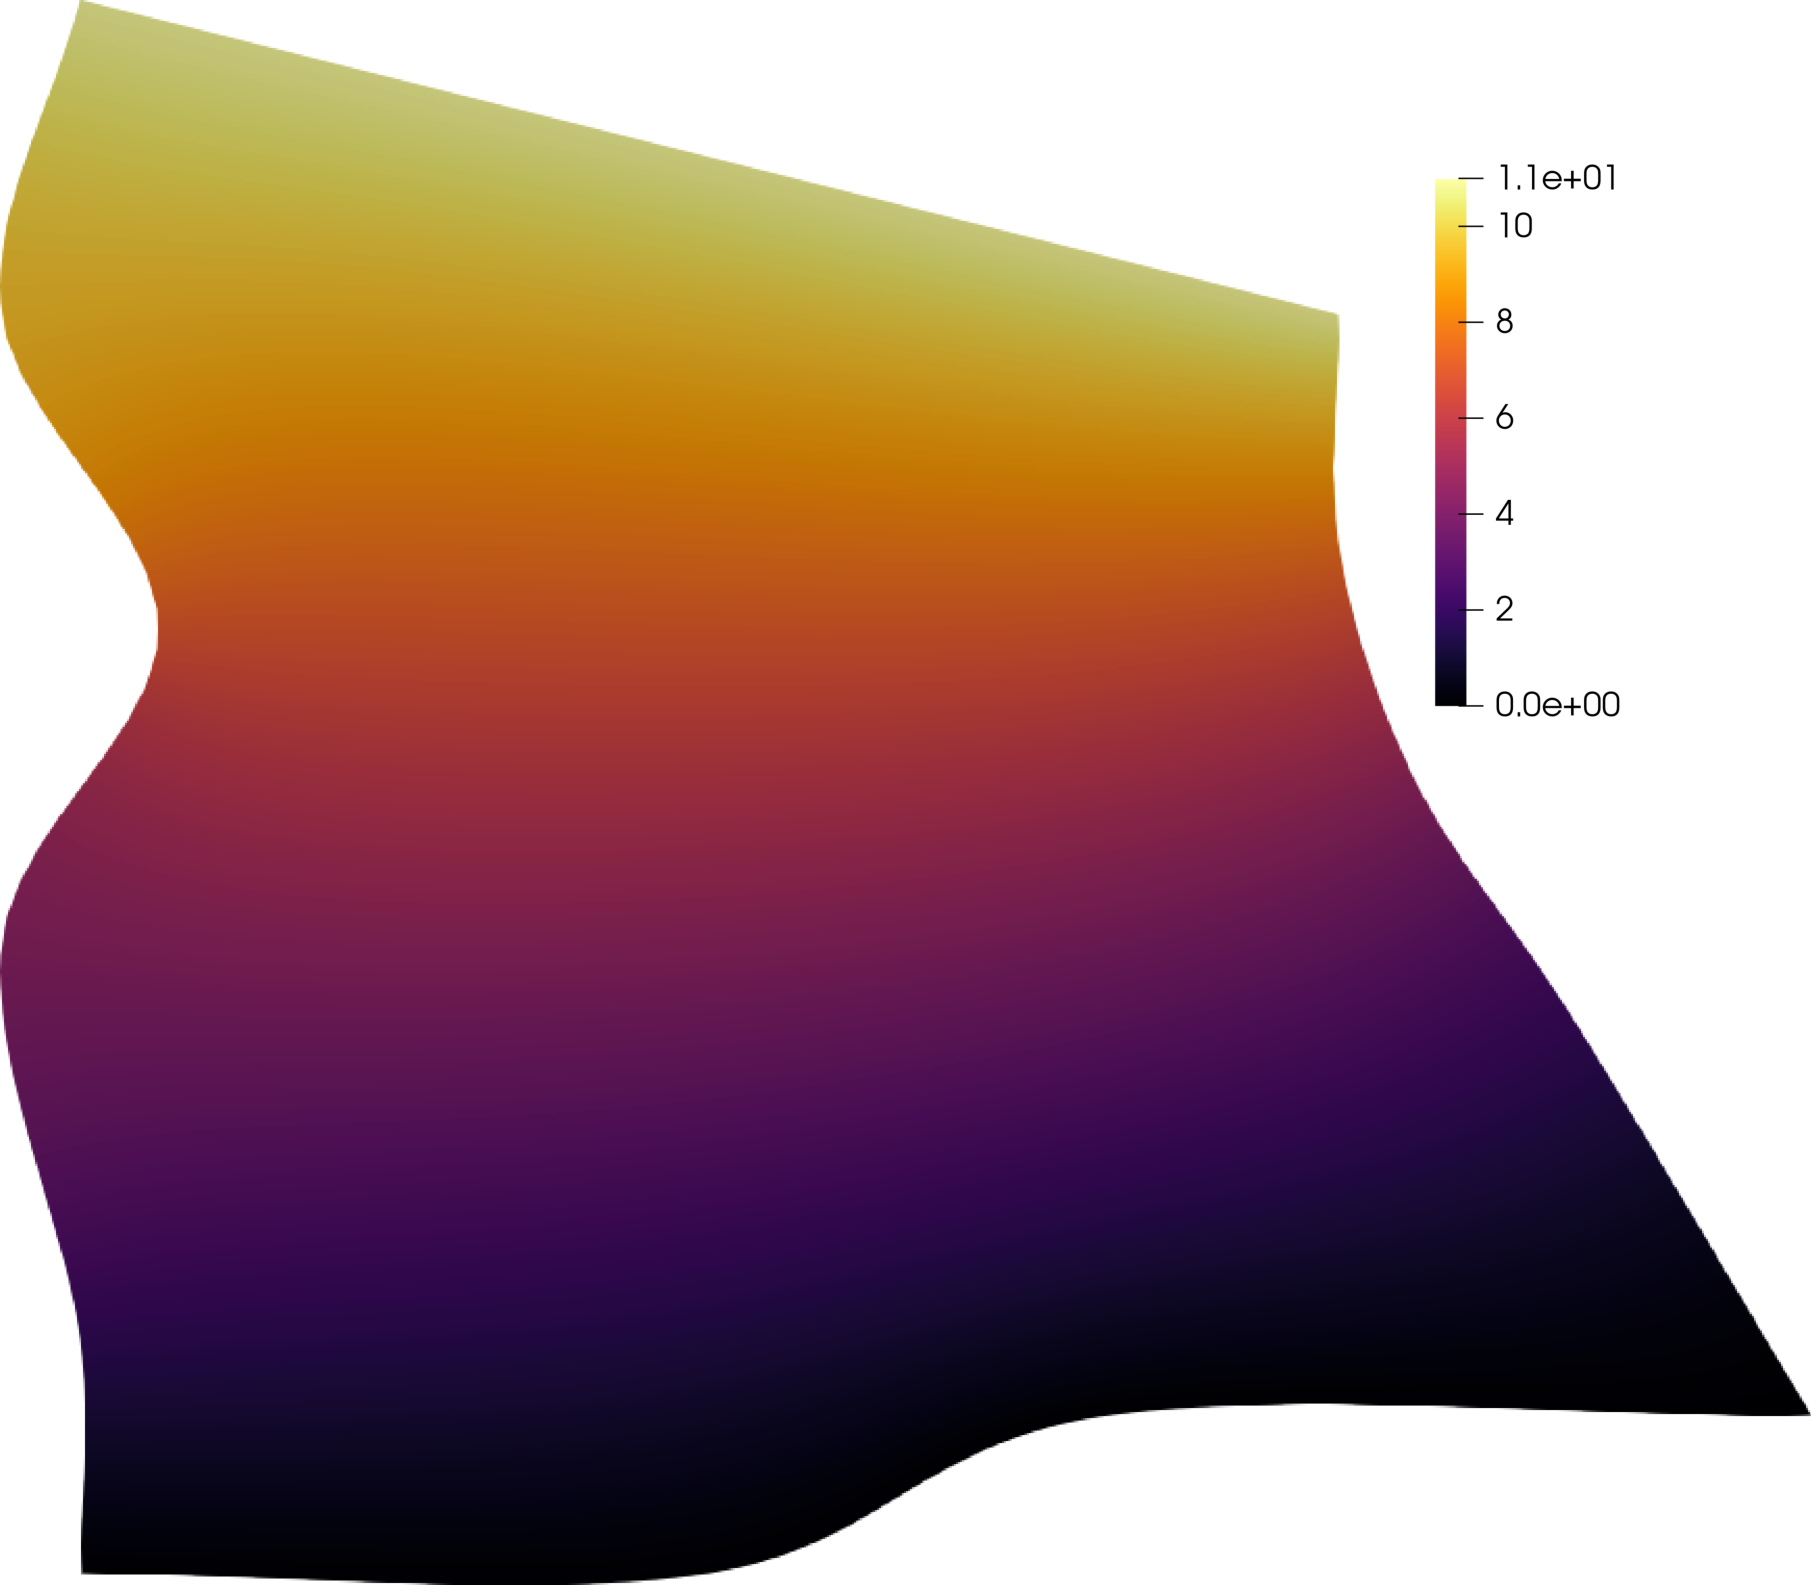
\includegraphics[width=\textwidth]{images/quad_equation_2.pdf}
    \caption{Champ scalaire $U$.}
    \label{fig:quad_equation_2}
\end{subfigure}
\hfill
\begin{subfigure}{0.44\textwidth}
    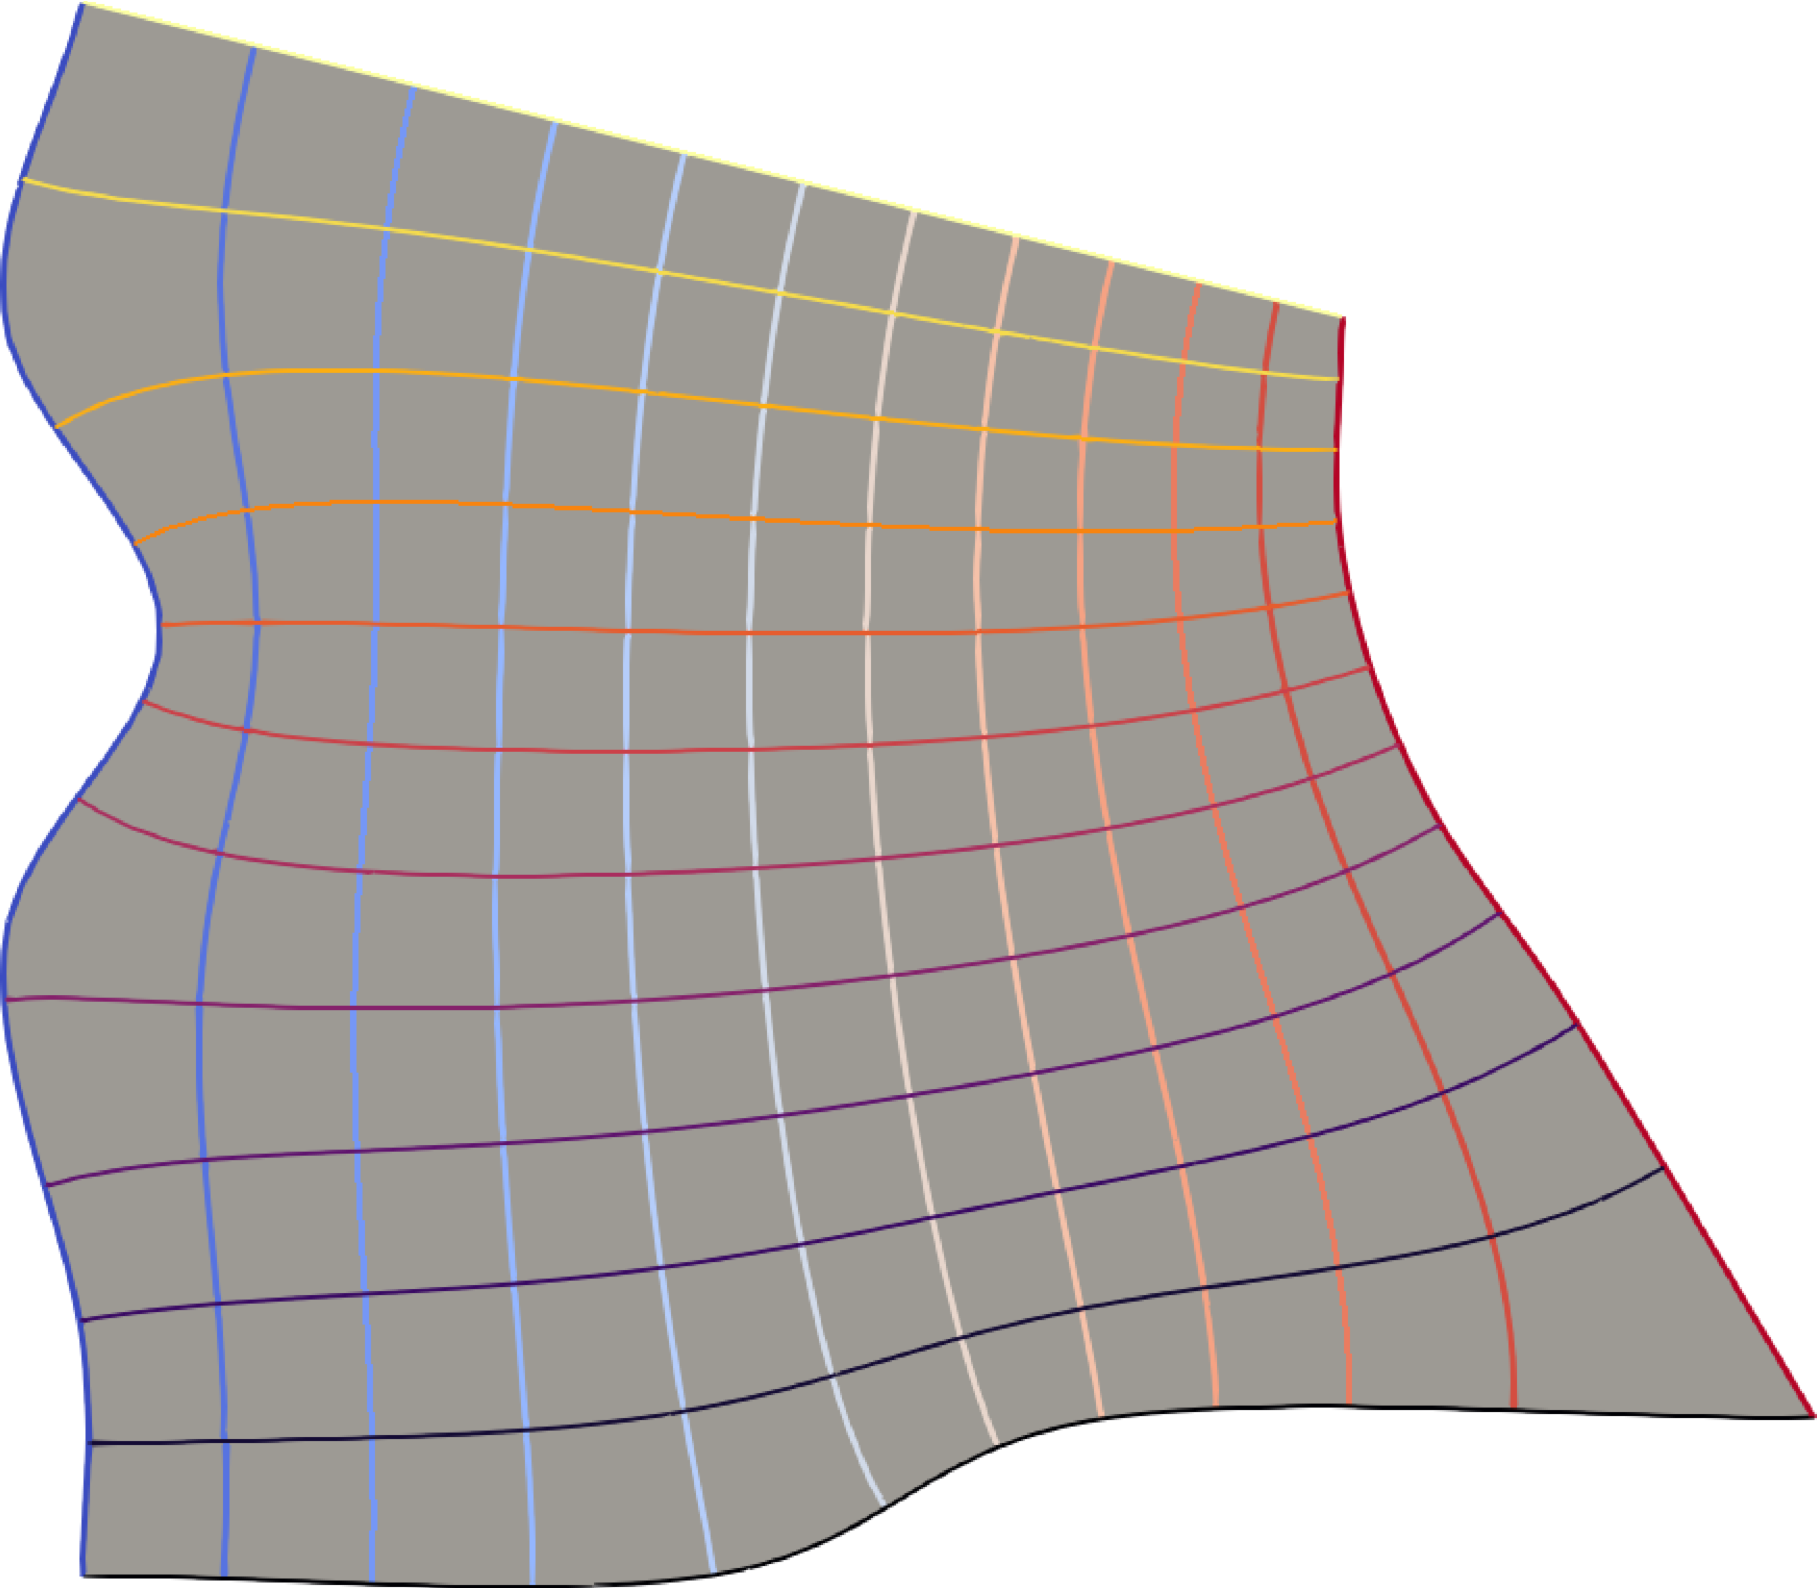
\includegraphics[width=\textwidth]{images/quad_equation_3.pdf}
    \caption{Lignes de niveau associées aux valeurs des nœuds de discrétisation situés sur le bord.}
    \label{fig:quad_equation_3}
\end{subfigure}
\\[0.2cm]
\begin{subfigure}{0.455\textwidth}
    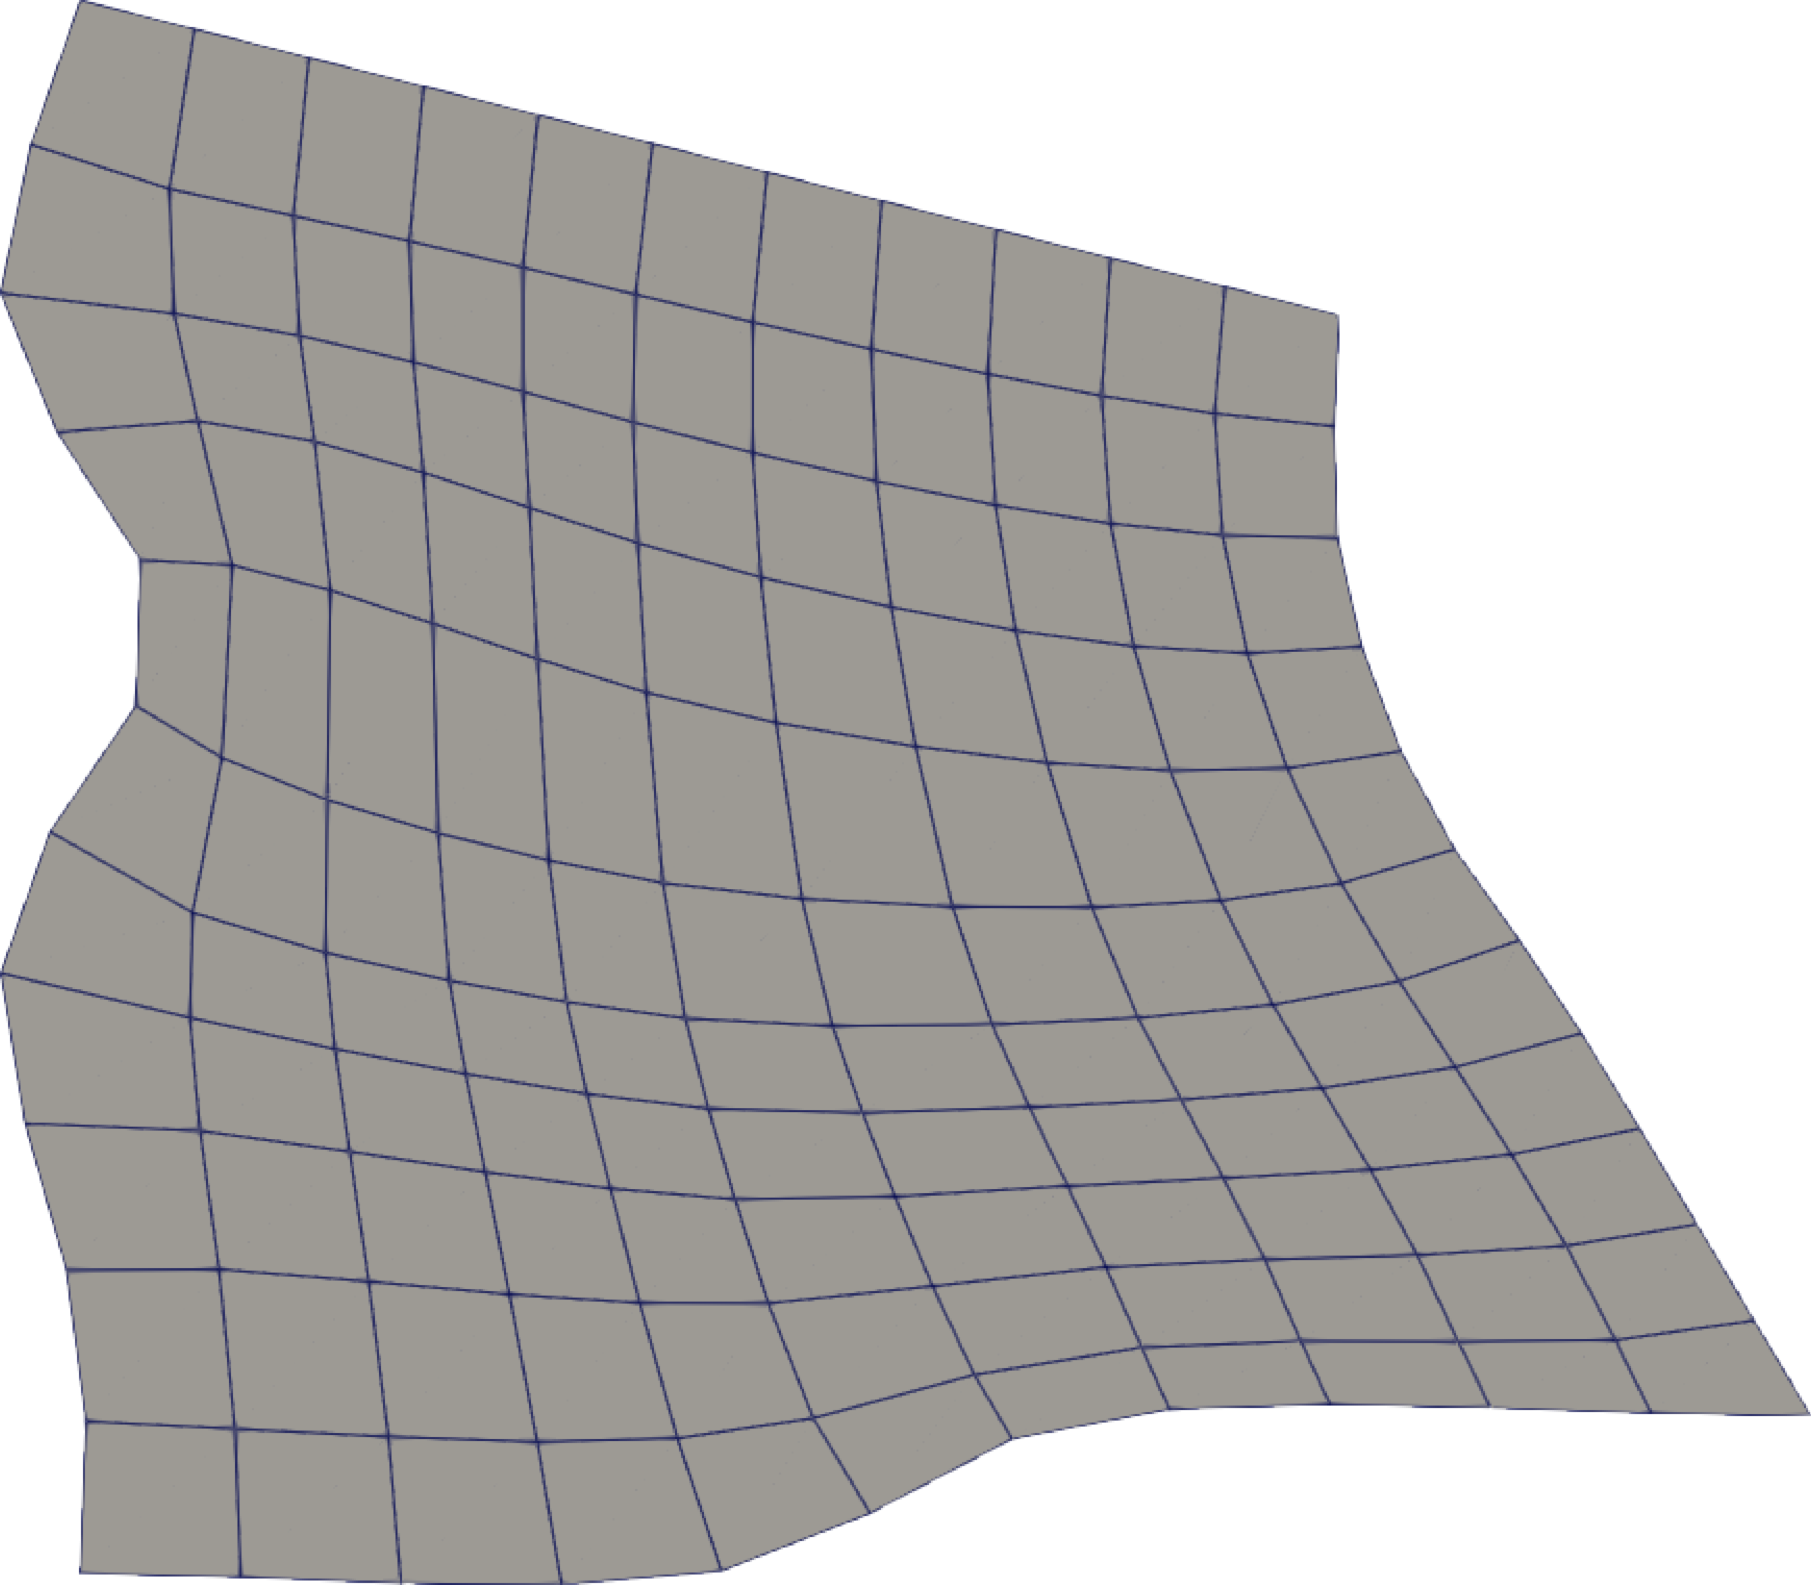
\includegraphics[width=\textwidth]{images/quad_equation_4.pdf}
    \caption{Maillage.}
    \label{fig:quad_equation_4}
\end{subfigure}
\caption{Illustration du maillage d'un bloc par résolution d'EDP.}
\label{fig:quad_equation}
\end{figure}

C'est cette dernière méthode que nous choisissons d'adopter dans notre implémentation en raison de sa simplicité, particulièrement dans le contexte d'une extension aux surfaces courbes dans l'espace (voir le chapitre \ref{chap:surface_courbe}). Le maillage du partitionnement présenté sur la figure \ref{fig:separatrice_echantillonage} est représenté sur la figure \ref{fig:maillage_quad_carre} à partir de cette méthode.

\begin{figure}[h!]
\centering
\begin{subfigure}{0.49\textwidth}
    \includegraphics[width=\textwidth]{images/quad_eclatement.pdf}
    %\caption{Insertion de $D$.}
    \label{fig:quad_eclatement}
\end{subfigure}
\hfill
\begin{subfigure}{0.49\textwidth}
    \includegraphics[width=\textwidth]{images/quad_carre.pdf}
    %\caption{Insertion de $E$.}
    \label{fig:quad_carre}
\end{subfigure}
\caption{Illustration du maillage des blocs résultant du partitionnement de l'exemple présenté à la figure \ref{fig:separatrice_echantillonage}.}
\label{fig:maillage_quad_carre}
\end{figure}


\section{Opération d'alignement}

Abordons à présent la discrétisation de l'opération d'alignement exposée dans le chapitre \ref{chap:theoritical}, en supposant que $\Omega$ soit un domaine simplement connexe. Pour rappel, cette opération vise à créer un champ de croix $\bar{v}=\mathbf{R}(\phi)\bar{u}$ aligné sur $\partial\Omega$ (c'est-à-dire aligné sur le champ de croix $\bar{n}$ associé à la normale sortante de $\partial\Omega$). Ceci est réalisé à partir d'un champ de croix $\bar{u}$ presque-$\mathcal{C}^1$ défini sur $\Omega$, mais non nécessairement aligné par rapport au bord de $\Omega$. La fonction $\phi$ est définie par l'équation \eqref{eqn:principe_def_phi}.

Considérons $\bar{u}_h$ comme une représentation discrète de $\bar{u}$ sur $\Omega_h$. Dans le contexte discret, cette opération équivaut à aligner $\bar{u}_h$ sur un champ de croix défini sur $\partial\Omega_h$ et représentant le champ de croix associé à la normale extérieure de $\partial\Omega$. Commençons par construire cette représentation que nous notons $\bar{n}_h$. Pour tout sommet $a\in S_h\cap\partial\Omega_h$, avec $b$ et $c$ comme ses sommets voisins également situés sur $\partial\Omega_h$, nous avons :
\begin{equation}
\bar{n}_h(a)=\displaystyle\left\{\mathbf{R}\left(\frac{m\pi}{2}\right)g(a),~ m\in\mathbb{Z}\right\},
\end{equation}
où $g(a)$ est donné par:
\begin{equation}
\label{eqn:n_reconstruit}
g(a)=\displaystyle\frac{1}{\|\overrightarrow{ab}+\overrightarrow{ac}\|}\left(\overrightarrow{ab}+\overrightarrow{ac}\right).
\end{equation}
Ensuite, on élimine les arêtes de bord où la variation angulaire $\delta\theta$ du champ $\bar{n}_h$ n'est pas définie, soit en effectuant un raffinement local ou global du maillage, soit en insérant dans le maillage un nouveau point situé au milieu de l'arête en question. Ce point sera considéré comme un point singulier dans le champ $\bar{n}_h$, et par conséquent, pour un tel point $a\in S_h\cap\partial\Omega_h$, nous fixons $\bar{n}_h(a)=0$. Ainsi, on se retrouve avec deux types d'arêtes incluses dans $\partial\Omega_h$ : les arêtes avec un sommet singulier dans $\bar{n}_h$ et les arêtes où la variation angulaire $\delta\theta$ de $\bar{n}_h$ est bien définie. La construction de $\bar{n}_h$ se poursuit alors de la manière suivante : pour tout point $p\in ab$ avec $ab$ une arête incluse dans $\partial\Omega_h$, on a:\\
\begin{itemize}
\item[$\bullet$] Si $\delta\theta(\bar{n}_h(a), \bar{n}_h(b))$ est défini, alors:
 $$
 \left\{
 \begin{array}{l}
 \bar{n}_h(p)=\mathbf{R}(\theta_p)\bar{n}_h(a),\\\\
 \theta_p = \theta_{\bar{n}_h}(a)+\displaystyle\frac{\|\overrightarrow{ap}\|}{\|\overrightarrow{ab}\|}\delta\theta(\bar{n}_h(a), \bar{n}_h(b)).
 \end{array}
 \right.
 $$
 \item[$\bullet$] Sinon, par construction, l'un des deux sommets de l'arête $ab$ est nul et l'autre non nul. Supposons sans perte de généralité qu'il s'agit de $a$. On pose alors:
 $$
 \bar{n}_h(p)=\bar{n}_h(b).
 $$
\end{itemize}
Après la construction du champ de croix $\bar{n}_h$, nous entamons l'opération d'alignement proprement dite. L'objectif est d'ajuster $\bar{u}_h$ pour former un nouveau champ de croix $\bar{v}_h$ tel que $\bar{v}_h=\bar{n}_h$ sur $\Omega_h$, à l'exception d'un nombre limité de points où il s'annule. En d'autres termes, nous visons à ce que, pour tout $p\in\partial\Omega_h$, $\bar{v}_h(p)\in\{\bar{n}_h(p), 0\}$. Pour y parvenir, nous débutons en associant à chaque sommet $p\in\partial S_h\cap\Omega_h$ un paramètre $I_p$ vérifiant:
\begin{equation}
I_p=\displaystyle\frac{k}{4}\mbox{ avec }k\in\mathbb{Z}\mbox{ et }k\leq 1.
\end{equation}
Ce paramètre représente l'indice désiré pour les points de bord dans le champ de croix $\bar{v}_h$ (une fois l'opération d'alignement réalisée). Un critère a priori pour choisir automatiquement ce paramètre a été exposé dans la sous-section \ref{subsec:sing_bord}. Ensuite, nous définissons l'ensemble $\mathcal{B}$ qui regroupe les points que nous souhaitons rendre singuliers dans le champ de croix $\bar{v}_h$ (une fois l'opération d'alignement réalisée). Cet ensemble doit, naturellement, inclure tous les points $p$ tels que $I_p\neq 0$, car ces points auront un indice non nul dans $\bar{v}_h$. Cependant, il est également envisageable d'inclure dans $\mathcal{B}$ des points dont le paramètre $I_p$ est nul, ce qui permet, par exemple, de délimiter des portions du bord du domaine. Cela offre la possibilité, une fois le maillage construit, d'y imposer des conditions aux limites pour la résolution d'une équation donnée. L'ensemble $\mathcal{B}$ doit aussi inclure les points singuliers du champ $\bar{n}_h$. Ces points étant déjà singulier dans $\bar{n}_h$, ils resteront singuliers dans $\bar{v}_h$ après l'opération d'alignement. Pour finir, il est impératif que le champ de croix $\bar{u}_h$ ainsi que l'ensemble $\mathcal{B}$ satisfassent:\\
\begin{itemize}
 \item[$\bullet$] $0\leq Card(\mathcal{S}_{\bar{u}_h})+Card(\mathcal{B}) <\infty$,\\
 \item[$\bullet$] pour tout point $p\in\mathcal{S}_{\bar{u}_h}$, $id_{\bar{u}_h}(p)=k/4$, avec $k\in\mathbb{Z}$ et $k\leq 1$,\\
 \item[$\bullet$] soit $\gamma$ une paramétrisation de $\partial\Omega_h$ dans le sens positif. Il existe $\theta_{\bar{u}_h}^\gamma$ vérifiant:
 \begin{equation}
    \label{eqn:etude_hyp_u_simple}
    \theta_{\bar{u}_h}^\gamma(1)-\theta_{\bar{u}_h}^\gamma(0)=\chi(\Omega_h)-\sum_{p\in\mathcal{B}}I_p.
\end{equation}
\end{itemize}
Ces critères sont automatiquement vérifiés si les points singuliers de $\bar{u}$ sont isolés et que le maillage $\Omega_h$ est adapté à la représentation discrète que nous avons présentée dans la sous-section \ref{sec:repr_discrete}. Le champ de croix $\bar{v}_h$ est alors défini pour tout $p\in\Omega_h$ par:
\begin{equation}
\bar{v}_h(p)=
\left\{
\begin{array}{ll}
\mathbf{R}(\phi_h(p))\bar{u}_h(p) & \mbox{ si } p\in\Omega_h\backslash(\mathcal{B}\cup\mathcal{S}_{\bar{u}_h}),\\[0.5cm]
\bar{n}_h(p) & \mbox{ si } p\in(\mathcal{S}_{\bar{u}_h}\cap\partial\Omega_h)\backslash\mathcal{B},\\[0.5cm]
0 & \mbox{ si } p\in\mathcal{B}.
\end{array}
\right.
\label{eqn:etude_def_v_second}
\end{equation}
où $\phi_h$ est définie par l'équation de Laplace suivant:
\begin{equation}
\left\{
\begin{array}{lcll}
\Delta\phi_h &=& 0 &\mbox{ dans }\Omega,\\[0.5cm]
\phi_h(\gamma(t))&=&\theta_{\bar{n}_h}^\gamma(t)+\mathcal{I}(t)-\theta_{\bar{u}_h}(\gamma(t))& \mbox{ sur } \gamma^{-1}(\partial\Omega_h\backslash(\mathcal{B}\cup\mathcal{S}_{\bar{u}_h})),
\end{array}
\right.
\label{eqn:algorithm_def_phi}
\end{equation}
où la fonction $\mathcal{I}$ est donnée par:
$$
\mathcal{I}(t)=\displaystyle\sum_{s\in\gamma^{-1}(\mathcal{B})}\left[\left(\pi-\widehat{\gamma(s)}-2\pi I_{\gamma(s)}\right)-\left(\displaystyle\lim\limits_{r\rightarrow s^+}\theta^{\gamma}_{\bar{n}_h}(r) - \lim\limits_{r\rightarrow s^-}\theta^{\gamma}_{\bar{n}_h}(r)\right)\right]\mathbb{1}_{[0, t]}(s),
$$
avec $\widehat{\gamma(s)}$ la mesure de l'ouverture angulaire de la frontière en $\gamma(s)$.

En pratique, la résolution de l'équation \eqref{eqn:algorithm_def_phi} est effectuée par la méthode des éléments finis $\mathbb{P}_1$, en utilisant la formule du Laplacien cotangente pour la discrétisation de l'opérateur Laplacien \cite{solomon2014laplace, nealen2006laplacian, belkin2008discrete} (voir Annexe \ref{Op_lap_discr} pour plus de détails). Cette approche est privilégiée en raison de sa simplicité, facilitant de plus l'extension de l'opération d'alignement dans le cas des surfaces courbes dans l'espace (voir le chapitre \ref{chap:surface_courbe}).

\begin{remark}
\[\]
\vspace{-1cm}
\begin{enumerate}
\item Le champ de croix $\bar{v}_h$ conserve certaines propriétés du champ de croix $\bar{u}_h$. Ainsi, on a $\mathcal{S}_{\bar{v}_h}\cap(\Omega_h\backslash\partial\Omega_h)=\mathcal{S}_{\bar{u}_h}\cap(\Omega_h\backslash\partial\Omega_h)$, puisque $\phi_h$ est $\mathcal{C}^0$ sur $\Omega_h\backslash\partial\Omega_h$. Les indices des points constituant ces ensembles sont également préservés. Autrement dit, pour tout point $p\in\Omega_h\backslash\partial\Omega_h$, on a $id_{\bar{u}_h}(p)=id_{\bar{v}_h}(p)$.
\item Pour tout $p\in\partial\Omega_h$, si $p\in S_h$, alors $id_{\bar{v}_h}(p)=I_p$ ; sinon, $id_{\bar{v}_h}
(p)=0$.
\item Lorsque $\Omega_h$ est un domaine non simplement connexe, la procédure d'alignement reste conforme à celle développée dans le chapitre \ref{chap:theoritical}. Il convient toutefois de définir avec précision $\bar{n}_h$ et $\mathcal{B}$ pour chaque composante connexe de $\partial\Omega_h$.
\end{enumerate}
\end{remark}
Nous présentons le processus d'alignement à travers un exemple illustré à la figure \ref{fig:alignment}.

\begin{figure}[h!]
\centering
\begin{subfigure}{0.5\textwidth}
    \includegraphics[width=\textwidth]{images/alignment_1.pdf}
    \caption{Champ de croix $\bar{u}_h$}
    \label{fig:alignment_1}
\end{subfigure}
\hfill
\begin{subfigure}{0.45\textwidth}
    \includegraphics[width=\textwidth]{images/alignment_2.pdf}
    \caption{Champ scalaire $\phi_h$ (en randian)}
    \label{fig:alignment_2}
\end{subfigure}
\\[0.1cm]
\begin{subfigure}{0.5\textwidth}
    \includegraphics[width=\textwidth]{images/alignment_3.pdf}
    \caption{Champ de croix $\bar{v}_h$.}
    \label{fig:alignment_3}
\end{subfigure}
\hfill
\begin{subfigure}{0.482\textwidth}
    \includegraphics[width=\textwidth]{images/alignment_4.pdf}
    \caption{Maillage.}
    \label{fig:alignment_4}
\end{subfigure}
\caption{Illustration du processus d'alignement dans un cadre discret.}
\label{fig:alignment}
\end{figure}


\section{Analyse de convergence}
\label{subsec:analyse_convergence}

Dans les sections précédentes, nous avons examiné la problématique du partitionnement d'un domaine défini par un maillage triangulaire, ainsi que celle de la génération d'un maillage quadrangulaire à partir du partitionnement ainsi construit. Cette section a pour objectif de démontrer que le maillage obtenu à partir du champ de croix résultant de l'opération d'alignement constitue effectivement un maillage du domaine initial $\Omega$. Pour cela, il suffit de démontrer que le partitionnement construit sur $\Omega_h$, que nous notons $\mathcal{P}_h$, converge vers un partitionnement de $\Omega$ comprenant des partitions quadrilatérales.\\\\
Soit $\bar{v}$ le champ de croix définit par:
\begin{equation}
\bar{v}(p)=
\left\{
\begin{array}{ll}
\mathbf{R}(\phi(p))\bar{u}(p) & \mbox{ si } p\in\Omega\backslash(\mathcal{B}\cup\mathcal{S}_{\bar{n}}\cup\mathcal{S}_{\bar{u}}),\\[0.5cm]
\bar{n}(p) & \mbox{ si } p\in(\mathcal{S}_{\bar{u}}\cap\partial\Omega)\backslash(\mathcal{B}\cup\mathcal{S}_{\bar{n}}),\\[0.5cm]
0 & \mbox{ si } p\in\mathcal{B}\cup\mathcal{S}_{\bar{n}}.
\end{array}
\right.
\label{eqn:continuous_def_v}
\end{equation}
où $\phi:\Omega\longrightarrow\mathbb{R}$ est définie comme la solution de l'équation de Laplace suivante:
\begin{equation}
\left\{
\begin{array}{lcll}
\Delta\phi &=& 0 &\mbox{ dans }\Omega,\\[0.5cm]
\phi(\gamma(t))&=&\theta_{\bar{n}}^\gamma(t)+\mathcal{I}(t)-\theta_{\bar{u}}(\gamma(t))& \mbox{ sur } \gamma^{-1}(\partial\Omega\backslash(\mathcal{B}\cup\mathcal{S}_{\bar{n}}\cup\mathcal{S}_{\bar{u}})),
\end{array}
\right.
\label{eqn:continuous_def_phi}
\end{equation}
où la fonction $\mathcal{I}$ est donnée pour tout $t\in\gamma^{-1}(\partial\Omega\backslash(\mathcal{B}\cup\mathcal{S}_{\bar{n}}\cup\mathcal{S}_{\bar{u}}))$ par:
$$
\mathcal{I}(t)=\sum_{s\in\gamma^{-1}(\mathcal{B}\cup\mathcal{S}_{\bar{n}})}\left[\left(\pi-\widehat{\gamma(s)}-2\pi I_{\gamma(s)}\right)-\left(\lim\limits_{r\rightarrow s^+}\theta^{\gamma}_{\bar{n}}(r) - \lim\limits_{r\rightarrow s^-}\theta^{\gamma}_{\bar{n}}(r)\right)\right]\mathbb{1}_{[0, t]}(s),
$$
avec $\widehat{\gamma(s)}$ représentant la mesure de l'ouverture angulaire de la frontière en $\gamma(s)$. Selon le théorème \ref{thm:theorem1} du chapitre \ref{chap:theoritical}, l'algorithme \ref{alg:algo_main} permet, en l'absence de convergence de séparatrices vers un cycle limite, de partir de $\bar{v}$ pour créer un partitionnement $\mathcal{P}$ de $\Omega$ tel que toutes les partitions soient formées par quatre séparatrices disjointes. Afin d'atteindre l'objectif énoncé, il est donc nécessaire de démontrer que les séparatrices du partitionnement $\mathcal{P}_h$ convergent vers les séparatrices du partitionnement $\mathcal{P}$ lorsque $h$ tend vers $0$.\\\\
Avant de montrer que ces deux familles de séparatrices convergent l'une vers l'autre, examinons d'abord ce qui se passe lorsque nous cherchons à voir si l'approximation d'une ligne de champ construite dans $\bar{v}_h$ converge vers une ligne de $\bar{v}$ ayant la même origine et la même direction de départ. Pour ce faire, notons $I$ l'opérateur d'intégration d'une ligne de champ et $I_h$ son approximation (par exemple la méthode de Heun). Ainsi $I(p,w,\bar{v})$ désigne la ligne de champ dans le champ $\bar{v}$ démarrant en $p$ dans la direction $w$ et $I_h(p,w,\bar{v})$ est l'approximation de cette ligne de champ. En supposant que $I_h$ a été discrétisé sur $t_1<\dots<t_n$, il vient, par la construction des lignes de champ (présentée dans la sous-section \ref{sub:sepa_constr}), que $t_{i+1}-t_i<h$ pour tout $i\in\llbracket 1, n\rrbracket$ avec $h$ le pas du maillage. $I_h$ étant une approximation consistante de $I$, on a:
$$||I(p,w,\bar{v})-I_h(p,w,\bar{v})||\xrightarrow[h \to 0]{} 0,$$
avec $$||I(p,w,\bar{v})-I_h(p,w,\bar{v})||=\max_{1 \leq i \leq n} |I(p,w,\bar{v})(t_i)-I_h(p,w,\bar{v})(t_i)|_2.$$
On peut maintenant comparer une ligne de champ du champ $\bar{v}$ d'origine $p$ et de vecteur initial $w$ (notée $I(p,w,\bar{v})$) et l'approximation d'une ligne de champ du champ $\bar{v}_h$ d'origine $p$ et de vecteur initial $w$ (notée $I_h(p,w,\bar{v}_h)$). On a:
\begin{eqnarray*}
||I(p,w,\bar{v})-I_h(p,w,\bar{v}_h)||&\leq& ||I(p,w,\bar{v})-I(p,w,\bar{v}_h)|| + ||I(p,w,\bar{v}_h)-I_h(p,w,\bar{v}_h)||\\\\
&\leq& ||I(p,w,\bar{v}_h)-I_h(p,w,\bar{v}_h)|| +\\\\
&&||I(p,w,[\mathbf{L}_{\Omega_h}^{\Omega}\bar{v}_h])-I(p,w,\bar{v}_h)||+\\\\
&&||I(p,w,\bar{v})-I(p,w,[\mathbf{L}_{\Omega_h}^{\Omega}\bar{v}_h])||
\end{eqnarray*}
Le premier terme à droite de l'inégalité tend vers $0$ lorsque $h$ tend vers $0$ puisque $I_h$ est une approximation consistante de $I$. Le second converge aussi vers $0$ puisque $\Omega_h$ tend vers $\Omega$. Pour le troisième terme, notons que, par construction, $[\mathbf{L}_{\Omega_h}^{\Omega}\bar{n}_h]$ converge vers $\bar{n}$ lorsque $h$ tend vers $0$, puisque $\Omega_h$ tend vers $\Omega$. Il en est de même pour le champ de croix initial $\bar{u}_h$ (voir la sous-section \ref{Lien_u_u_h}). Ainsi, le problème \eqref{eqn:algorithm_def_phi} constitue une approximation du problème \eqref{eqn:continuous_def_v}. Par conséquent, on a $[\mathbf{L}_{\Omega_h}^{\Omega}\theta_{\bar{v}_h}]=[\mathbf{L}_{\Omega_h}^{\Omega}(\phi_h+\theta_{\bar{u}_h})]$ qui tend vers $\theta_{\bar{v}}=\phi+\theta_{\bar{u}}$. En d'autres termes, le champ de croix $[\mathbf{L}_{\Omega_h}^{\Omega}\bar{v}_h]$ converge vers le champ de croix $\bar{v}$ sur $\Omega_h$. Il vient alors que :
$$||I(p,w,\bar{v})-I(p,w,[\mathbf{L}_{\Omega_h}^{\Omega}\bar{v}_h])||\xrightarrow[h \to 0]{} 0,$$
Finalement on a:
$$||I(p,w,\bar{v})-I_h(p,w,\bar{v}_h)||\xrightarrow[h \to 0]{} 0.$$
On en déduit alors que les séparatrices approchées de $\bar{v}_h$ internes à $\Omega_h$ convergent vers les séparatrices de $\bar{v}$ internes à $\Omega$, étant donné que. En effet, étant donné que $[\mathbf{L}_{\Omega_h}^{\Omega}\bar{v}_h]$ converge vers $\bar{v}$, l'ensemble des points singuliers de $\bar{v}_h$ converge vers l'ensemble des points singuliers de $\bar{v}$ et, de plus, les directions de sortie des séparatrices de $\bar{v}_h$ calculées avec la fonction $W^\gamma_{\bar{v}_h}$ convergent vers les directions de sortie des séparatrices de $\bar{v}$.\\\\
Pour la convergence des séparatrices de bord, deux analyses sont possibles. Premièrement, comme $\Omega_h$ tend vers $\Omega$ lorsque $h$ tend vers $0$, il en va de même pour $\partial\Omega_h$, qui converge vers $\partial\Omega$. Ainsi, en considérant $\partial\Omega_h$ comme une approximation de la séparatrice de bord de $\bar{v}_h$, on obtient la convergence recherchée.\\\\
Une analyse plus approfondie consiste à ne pas considérer $\partial\Omega_h$ comme la séparatrice de bord de $\bar{v}_h$. Remarquons que le champ de croix $\bar{n}_h$ n'est pas aligné avec $\partial\Omega_h$. Nous définissons alors le domaine $\widetilde{\Omega_h}$ dont le bord $\partial\widetilde{\Omega_h}$ est aligné avec le champ de croix $\bar{n}_h$. Ainsi, les séparatrices de bord de $\bar{v}_h$ sont maintenant données (sans approximation) par le bord $\partial\widetilde{\Omega_h}$ de $\widetilde{\Omega_h}$. Notons que $[\mathbf{L}_{\Omega_h}^{\widetilde{\Omega_h}}\bar{v}_h]$ converge vers $\bar{v}_h$, puisque $[\mathbf{L}_{\Omega_h}^{\Omega}\bar{v}_h]$ converge vers $\bar{v}_h$. Il en découle que les séparatrices de $[\mathbf{L}_{\Omega_h}^{\widetilde{\Omega_h}}\bar{v}_h]$ convergent vers les séparatrices de $\bar{v}$, y compris les séparatrices de bord qui correspondent au bord $\partial\widetilde{\Omega_h}$ de $\widetilde{\Omega_h}$. L'intérêt d'une telle analyse réside dans le fait qu'elle permet, en pratique, de reconstruire une approximation d'ordre élevé du bord de $\Omega_h$ (voir la section \ref{sec:perspectives}).

\section{Génération de champ de croix}
\label{subsec:gen_cross_field}

Nous terminons ce chapitre en exposant quelques méthodes de génération de champ de croix que l'on rencontre dans la littérature. Dans notre travail, nous avons notemment utilisé ces méthodes pour créer les champ de croix initiaux qui sont le point d'entrée de notre opération d'alignement.

\subsection{L'Equation de Laplace}
\label{subsec:laplace_equation_generation}

L'idée principale de cette méthode, telle que décrite dans \cite{kowalski2013pde}, consiste à propager dans le domaine de calcul un champ de vecteur unitaire prescrit sur la frontière. On formule alors cette construction dans la résolution de l'équation de Laplace avec des conditions de Dirichlet sur la frontière données par les croix associées aux normales sortantes. Étant donné que l'ensemble des champs de croix ne forme pas un espace vectoriel, on utilise à la place un champ de représentation donné par:
$$
\mathcal{R}: \mathbf{c}\in\mathbf{C}\mapsto\mathcal{R}(\mathbf{c})=
\left\{
\begin{array}{ll}
\mathbf{R}(4\theta_{\mathbf{c}})(1, 0)^t& \mbox{ si }\mathbf{c}\neq 0,\\\\
0&\mbox{ sinon}.
\end{array}
\right.
$$
L'opération inverse est donné par:
$$
\mathcal{R}^{-1}: u=(u^1, u^2)\in\mathbb{R}^2\mapsto\mathcal{R}^{-1}(u)=
\left\{
\begin{array}{ll}
\displaystyle\left\{\mathbf{R}\left(\frac{m\pi}{2}+\frac{atan2(u^2, u^1)}{4}\right)(1, 0)^t,~ m\in \mathbb{Z}\right\} &\mbox{ si }u\neq (0,0),\\\\
0&\mbox{ sinon}.
\end{array}
\right.
$$
L'équation de propagation est alors donné par:
\begin{equation}
\left\{
\begin{array}{lcll}
\Delta u_r &=& 0 &\mbox{ dans }\Omega,\\\\
u_r(p)&=&\mathcal{R}(\bar{n}) & \mbox{ sur } \partial\Omega,
\end{array}
\right.
\label{eqn:frey_vectoriel}
\end{equation}
où $\Omega$ est le domaine de calcul et pour tout $p\in\Omega$, on a posé $u_r=\mathcal{R}(\bar{u})$. L'équation \eqref{eqn:frey_vectoriel} est une équation vectoriel qui peut être vu comme deux équation scalaire:
$$
\left\{
\begin{array}{lcll}
\Delta u_r^1 &=& 0 &\mbox{ dans }\Omega,\\\\
u_r^1(p)&=&\mathcal{R}(\bar{n}).(1, 0)^t & \mbox{ sur } \partial\Omega.
\end{array}
\right.
\quad\quad\quad
\left\{
\begin{array}{lcll}
\Delta u_r^2 &=& 0 &\mbox{ dans }\Omega,\\[0.5cm]
u_r^2(p)&=&\mathcal{R}(\bar{n}).(0, 1)^t & \mbox{ sur } \partial\Omega.
\end{array}
\right.
$$
En pratique, ces équations sont approchées en utilisant la méthode des éléments finis de Galerkin appliquée à un maillage triangulaire $\Omega_h$ de $\Omega$ avec des éléments $P_1$-Lagrange. On assemble ensuite $u_r$ puis on reconstitu $\bar{u}$ pour tout $p\in\Omega$ par:
$$
\bar{u}(p)=\mathcal{R}^{-1}(u_r(p)).
$$
On obtient un champ de croix aligné sur le bord du domaine de calcul et dont les point singulier de bord correspondent à une rotation minimale du champ de croix dans le voisinnage du point.

Dans la littérature, \cite{beaufort2017computing, viertel2019approach}, cette équation est souvent contrainte en imposant l'unitarité de la norme des croix du champ de croix. Cependant, le problème n'a alors pas de solution. Par pénalisation, on se retrouve alors avec l'équation de Ginzburg-Landau. Dans \cite{bethuel1994ginzburg}, les auteurs montrent qu'il existe des solutions généralisées pour cette équation.

Dans notre travail, nous n'imposons pas cette contrainte car nous nous intéressons simplement à l'orientation des croix, quitte à renormaliser ces croix après la résolution de l'équation de Laplace.



\subsection{Une expression analytique}

Nous donnons ici une expression analytique pour la construction de champ de croix sur $\Omega$.\\
\begin{itemize}
\item Soit un ensemble de points $(a_i)_{i\in I}\subset\Omega$, $I\subset\mathbb{N}$,\\
\item Soit associé à chaque $a_i$ pour tout $i\in I$, une valeur $k_i$ telle que $4k_i\in\mathbb{Z}$,\\
\item Soit $g:\Omega\longrightarrow\mathbb{S}^1\cup\{(0,0)\}$ défini pour tout $p\in\Omega$ par:\\
\begin{equation}
g(p)=
\left\{
\begin{array}{ll}
\mathbf{R}\left(\displaystyle\sum_{i\in I} k_i\arg{\overrightarrow{a_ip}}\right)(1,~0)^t&\mbox{ si }p\neq a_i,~i\in I,\\\\
(0,~0) &\mbox{ sinon}.
\end{array}
\right.
\end{equation}
\end{itemize}
alors l'application $\bar{u}$ définie pour tout $p\in\Omega$ par:\\
\begin{equation}
\bar{u}(p)=
\left\{
\begin{array}{ll}
\displaystyle\left\{\mathbf{R}\left(\frac{m\pi}{2}\right)g(p),~ m\in \mathbb{Z}\right\} &\mbox{ si }g(p)\neq (0,0),\\\\
0& \text{ sinon},
\end{array}
\right.
\end{equation}
est un champ de croix dont les points singuliers sont localisés aux points $(a_i)_{i\in I}$ tel que chaque point $a_i$, $i\in I$ est d'indice $k_i$.

Il est important de souligner que cette construction offre une grande souplesse dans l'établissement du champ, contrairement à l'approche précédente. Elle permet un contrôle précis sur la position des points singuliers dans le domaine ainsi que sur leurs indices. Cependant, le champ de croix ainsi obtenu n'est pas déterminé par le domaine sur lequel il est construit. Par conséquent, contrairement à l'approche précédente, le champ de croix peut ne pas être aligné. Ainsi, il est nécessaire d'appliquer l'approche d'alignement présentée précédemment pour orienter le champ par rapport au domaine que l'on souhaite mailler.

\section{Homogeneisation}
\label{sec:Homogeneisation_algo}

Comme évoqué dans l'introduction \ref{thesis_target}, les champs de croix générés en propageant la normale de l'extérieur vers l'intérieur du domaine (voir sous-section \ref{thesis_target} et \cite{kowalski2013pde}) peuvent donner lieu à une distribution de singularités susceptible de conduire à un partitionnement invalide ou non souhaité. À titre d'exemple, le champ de croix illustré dans la figure \ref{fig:non_homogene_cross_field} présente des points singuliers très rapprochés, entraînant une partition non homogène. Cela se traduit par des mailles de tailles très inégales dans le maillage final obtenu, comme illustré dans la figure \ref{fig:non_homogene_mesh_quad}. Dans cette section, nous proposons d'apporter des modifications au maillage résultant afin de remédier à cette problématique, tout en préservant la configuration en blocs structurés du maillage.\\\\
Nous procédons à l'optimisation du maillage quadrilatéral en recourant à une méthode appelée CVT, pour \emph{Centroid Voronoi Tesselation} (voir \cite{chen2004mesh}). Cet algorithme, de nature locale, vise à améliorer la qualité du maillage, notamment la régularité de la forme. Il opère en ajustant la position d'un sommet $s$ au sein de son patch local $T_{s}$, qui englobe tous les simplex contenant $s$, sans altérer la connectivité. Ainsi, le sommet $s$ se transforme en $s^*$, défini par:
$$s^*=\displaystyle\frac{1}{\displaystyle\sum_{T\in T_s}|T|}\left(\displaystyle\sum_{T\in T_s}b_T|T|\right),$$
où $b_T=\frac{\sum_{i=1}^3s_i}{3}$ représente le barycentre du triangle $T$ et $(s_i)_{i\in\llbracket 1, 3\rrbracket}$ désigne les sommets de $T$. Cette transformation est mise en œuvre pour optimiser localement la qualité du maillage sans altérer la connectivité. La figure \ref{fig:non_homogene} illustre le processus d'optimisation appliqué au maillage initialement présenté dans la figure \ref{fig:homogene}. Un exemple supplémentaire est proposé dans la figure \ref{fig:homo_demiDisc}.

\begin{figure}[h!]
\centering
\begin{subfigure}{0.49\textwidth}
    \includegraphics[width=\textwidth]{images/non_homo_cross_field.pdf}
    \caption{Champ de croix.}
    \label{fig:non_homogene_cross_field}
\end{subfigure}
\hfill
\begin{subfigure}{0.46\textwidth}
    \includegraphics[width=\textwidth]{images/non_homo_mesh_quad.pdf}
    \caption{Maillage quadrilatéral}
    \label{fig:non_homogene_mesh_quad}
\end{subfigure}
\caption{Exemple d'un maillage non homogène.}
\label{fig:non_homogene}
\end{figure}



\begin{figure}[h!]
\centering
\includegraphics[scale=0.34]{images/homogeneiser.pdf}
\caption{Homogénéisation du maillage présenté sur la figure \ref{fig:non_homogene}.}
\label{fig:homogene}
\end{figure}

\begin{figure}[h!]
\centering
\begin{subfigure}{0.65\textwidth}
    \includegraphics[width=\textwidth]{images/non_homo_demiDisc.pdf}
    \caption{Maillage non-homogène du demi disque.}
    \label{fig:homo_demiDisc_1}
\end{subfigure}
\\[0.5cm]
\begin{subfigure}{0.65\textwidth}
    \includegraphics[width=\textwidth]{images/homo_sans_bord_demiDisc.pdf}
    \caption{Homogénéisation sans prise en compte du bord.}
    \label{fig:homo_demiDisc_2}
\end{subfigure}
\\[0.5cm]
\begin{subfigure}{0.65\textwidth}
    \includegraphics[width=\textwidth]{images/homo_avec_bord_demiDisc.pdf}
    \caption{Homogénéisation complète}
    \label{fig:homo_demiDisc_3}
\end{subfigure}
\caption{Illustration du processus d'homogénéisation sur un autre exemple.}
\label{fig:homo_demiDisc}
\end{figure}
